\chapter{寮曡█涓庢暟瀛﹀熀纭€}

\section{璇剧▼绠€浠媫

鏁板鐗╃悊鏂圭▼鏄爺绌剁墿鐞嗙幇璞′腑鍑虹幇鐨勫亸寰垎鏂圭▼鍙婂叾姹傝В鏂规硶鐨勫绉戙€傚畠杩炴帴浜嗘暟瀛︾悊璁轰笌鐗╃悊搴旂敤锛屾槸鐞嗚鐗╃悊銆佸簲鐢ㄦ暟瀛︺€佸伐绋嬬瀛︾瓑棰嗗煙鐨勯噸瑕佸熀纭€銆?
\intro{鏈珷灏嗕粙缁嶆暟瀛︾墿鐞嗘柟绋嬬殑鍩烘湰姒傚康銆佺爺绌跺璞″拰涓昏姹傝В鏂规硶锛屽苟鍥為【鎵€闇€鐨勬暟瀛﹀熀纭€鐭ヨ瘑銆倉

\section{鏁板鐗╃悊鏂圭▼鐨勭爺绌跺璞

鏁板鐗╃悊鏂圭▼涓昏鐮旂┒涓夌被鍏稿瀷鐨勫亸寰垎鏂圭▼锛?
\\begin{mydefinition}[title={涓夊ぇ鍏稿瀷鏂圭▼}]
\begin{enumerate}
    \item \textbf{娉㈠姩鏂圭▼}锛堝弻鏇插瀷锛夛細
    \[
    \frac{\partial^2 u}{\partial t^2} = a^2 \lapl u
    \]
    鎻忚堪鎸姩銆佸０娉€佺數纾佹尝绛夋尝鍔ㄧ幇璞°€?    
    \item \textbf{鐑紶瀵兼柟绋媫锛堟姏鐗╁瀷锛夛細
    \[
    \frac{\partial u}{\partial t} = k \lapl u
    \]
    鎻忚堪鐑墿鏁ｃ€佺墿璐ㄦ墿鏁ｇ瓑鑰楁暎杩囩▼銆?    
    \item \textbf{鎷夋櫘鎷夋柉鏂圭▼}锛堟き鍦嗗瀷锛夛細
    \[
    \lapl u = 0
    \]
    鎻忚堪绋虫€佹俯搴﹀垎甯冦€侀潤鐢靛満銆佸紩鍔涘満绛夊钩琛＄姸鎬併€?\end{enumerate}
\end{mydefinition}

\begin{tikzpicture}
\begin{axis}[
    width=10cm,
    height=6cm,
    xlabel={$x$},
    ylabel={$u(x,t)$},
    title={娉㈠姩鏂圭▼瑙ｇ殑绀烘剰鍥緘,
    legend pos=north east,
    grid=major
]
\addplot[blue,thick,domain=0:4*pi,samples=100] {sin(deg(x))*exp(-0.1*deg(x))};
\addplot[red,thick,domain=0:4*pi,samples=100] {cos(deg(x))*exp(-0.1*deg(x))};
\legend{$u_1$,$u_2$}
\end{axis}
\end{tikzpicture}

\section{姹傝В鏂规硶姒傝堪}

鏁板鐗╃悊鏂圭▼鐨勪富瑕佹眰瑙ｆ柟娉曞寘鎷細

\begin{enumerate}
    \item \textbf{鍒嗙鍙橀噺娉晑锛氬皢鍋忓井鍒嗘柟绋嬭浆鍖栦负甯稿井鍒嗘柟绋嬫眰瑙?    \item \textbf{绉垎鍙樻崲娉晑锛氬埄鐢ㄥ倕閲屽彾鍙樻崲銆佹媺鏅媺鏂彉鎹㈢畝鍖栨柟绋?    \item \textbf{鏍兼灄鍑芥暟娉晑锛氬埄鐢ㄦ牸鏋楀嚱鏁版瀯閫犵壒瑙?    \item \textbf{鍙樺垎娉晑锛氬皢寰垎鏂圭▼闂杞寲涓烘硾鍑芥瀬鍊奸棶棰?    \item \textbf{鏁板€艰В娉晑锛氭湁闄愬樊鍒嗘硶銆佹湁闄愬厓娉曠瓑
\end{enumerate}

\section{鏁板鍩虹鍥為【}

\subsection{鍚戦噺鍒嗘瀽}

\\begin{mydefinition}[title={姊害銆佹暎搴︺€佹棆搴
璁?$u$ 涓烘爣閲忓満锛?\vect{F} = (F_1, F_2, F_3)$ 涓哄悜閲忓満锛?\begin{align}
    \grad u &= \left( \frac{\partial u}{\partial x}, \frac{\partial u}{\partial y}, \frac{\partial u}{\partial z} \right) \\
    \divg \vect{F} &= \frac{\partial F_1}{\partial x} + \frac{\partial F_2}{\partial y} + \frac{\partial F_3}{\partial z} \\
    \curl \vect{F} &= \begin{vmatrix}
    \vect{i} & \vect{j} & \vect{k} \\
    \frac{\partial}{\partial x} & \frac{\partial}{\partial y} & \frac{\partial}{\partial z} \\
    F_1 & F_2 & F_3
    \end{vmatrix}
\end{align}
\end{mydefinition}

\begin{myTheorem}[姊害銆佹暎搴︺€佹棆搴︾殑鍩烘湰鎬ц川}]
\begin{align}
    \curl(\grad u) &= \vect{0} \\
    \divg(\curl \vect{F}) &= 0 \\
    \lapl u &= \divg(\grad u)
\end{align}
\end{myTheorem}

\subsection{绉垎瀹氱悊}

\begin{myTheorem}[楂樻柉鏁ｅ害瀹氱悊]
璁?$\Omega$ 鏄?$\mathbb{R}^3$ 涓殑鏈夌晫闂尯鍩燂紝$\partial\Omega$ 鏄叾鍏夋粦杈圭晫锛?\vect{F}$ 鍦?$\Omega$ 涓婅繛缁彲寰紝鍒欙細
\[
\iiint_{\Omega} \divg \vect{F} \, dV = \oiint_{\partial\Omega} \vect{F} \cdot d\vect{S}
\]
\end{myTheorem}

\begin{myTheorem}[鏍兼灄绗竴鍏紡]
璁?$u, v$ 鍦?$\Omega$ 涓婁簩闃惰繛缁彲寰紝鍒欙細
\[
\iiint_{\Omega} (u \lapl v + \grad u \cdot \grad v) \, dV = \oiint_{\partial\Omega} u \frac{\partial v}{\partial n} \, dS
\]
鍏朵腑 $\frac{\partial v}{\partial n}$ 鏄?$v$ 娌垮娉曞悜鐨勬柟鍚戝鏁般€?\end{myTheorem}

\subsection{鍌呴噷鍙剁骇鏁皚

\\begin{mydefinition}[title={鍌呴噷鍙剁骇鏁癩
璁?$f(x)$ 鍦?$[-L, L}]$ 涓婃弧瓒崇媱鍒╁厠闆锋潯浠讹紝鍒欙細
\[
f(x) = \frac{a_0}{2} + \sum_{n=1}^{\infty} \left( a_n \cos\frac{n\pi x}{L} + b_n \sin\frac{n\pi x}{L} \right)
\]
鍏朵腑锛?\begin{align}
    a_n &= \frac{1}{L} \int_{-L}^{L} f(x) \cos\frac{n\pi x}{L} \, dx, \quad n = 0, 1, 2, \ldots \\
    b_n &= \frac{1}{L} \int_{-L}^{L} f(x) \sin\frac{n\pi x}{L} \, dx, \quad n = 1, 2, \ldots
\end{align}
\end{mydefinition}

\begin{lstlisting}[language=Python, caption={Fourier Series Approximation}]
import numpy as np
import matplotlib.pyplot as plt

def fourier_series(x, n_terms):
    result = 0
    for n in range(1, n_terms + 1):
        result += ((-1)**(n+1)) * np.sin(n * x) / n
    return result

x = np.linspace(-np.pi, np.pi, 1000)
f_true = x

plt.figure(figsize=(10, 6))
plt.plot(x, f_true, 'k-', label=r'$f(x)=x$', linewidth=2)

for n_terms in [1, 3, 5, 10]:
    f_approx = fourier_series(x, n_terms)
    plt.plot(x, f_approx, label=f'{n_terms} terms')

plt.xlabel('$x$')
plt.ylabel('$f(x)$')
plt.title('Fourier Series Approximation')
plt.legend()
plt.grid(True)
plt.show()
\end{lstlisting}

\section{鐗╃悊鑳屾櫙}

\subsection{寮︽尟鍔ㄩ棶棰榼

鑰冭檻涓€鏍归暱搴︿负 $L$ 鐨勫脊鎬у鸡锛屽叾妯悜鎸姩婊¤冻娉㈠姩鏂圭▼锛?\[
\frac{\partial^2 u}{\partial t^2} = a^2 \frac{\partial^2 u}{\partial x^2}
\]
鍏朵腑 $a = \sqrt{T/\rho}$锛?T$ 鏄紶鍔涳紝$\rho$ 鏄嚎瀵嗗害銆?
\subsection{鐑紶瀵奸棶棰榼

鑰冭檻涓€涓潎鍖€缁嗘潌鐨勭儹浼犲锛屾俯搴﹀垎甯冩弧瓒筹細
\[
\frac{\partial u}{\partial t} = k \frac{\partial^2 u}{\partial x^2}
\]
鍏朵腑 $k = K/(\rho c)$ 鏄儹鎵╂暎绯绘暟锛?K$ 鏄儹瀵肩巼锛?\rho$ 鏄瘑搴︼紝$c$ 鏄瘮鐑銆?
\subsection{闈欑數鍦洪棶棰榼

鐪熺┖涓潤鐢靛満鐨勭數鍔挎弧瓒虫媺鏅媺鏂柟绋嬶紙鏃犵數鑽峰尯鍩燂級鎴栨硦鏉炬柟绋嬶紙鏈夌數鑽峰尯鍩燂級锛?\[
\lapl \varphi = -\frac{\rho}{\varepsilon_0}
\]
鍏朵腑 $\rho$ 鏄數鑽峰瘑搴︼紝$\varepsilon_0$ 鏄湡绌轰粙鐢靛父鏁般€?
\section{鏈珷灏忕粨}

鏈珷浠嬬粛浜嗘暟瀛︾墿鐞嗘柟绋嬬殑鍩烘湰姒傚康鍜岀爺绌跺璞★紝鍥為【浜嗗悜閲忓垎鏋愩€佺Н鍒嗗畾鐞嗗拰鍌呴噷鍙剁骇鏁扮瓑鏁板鍩虹锛屽苟缁欏嚭浜嗗嚑涓吀鍨嬬殑鐗╃悊搴旂敤鑳屾櫙銆?
\begin{myremark}
鏁板鐗╃悊鏂圭▼鐨勬牳蹇冩€濇兂鏄皢鐗╃悊闂杞寲涓烘暟瀛︽ā鍨嬶紙鍋忓井鍒嗘柟绋嬶級锛岀劧鍚庨€氳繃鍚勭鏁板鏂规硶姹傝В锛屾渶鍚庡皢鏁板瑙ｈВ閲婁负鐗╃悊鐜拌薄銆?\end{myremark}

\begin{enumerate}
    \item 涓夊ぇ鍏稿瀷鏂圭▼鍒嗗埆鎻忚堪浜嗘尝鍔ㄣ€佹墿鏁ｅ拰骞宠　涓夌被鐗╃悊杩囩▼銆?    \item 鍒嗙鍙橀噺娉曟槸鏈€鍩烘湰鐨勬眰瑙ｆ柟娉曪紝閫傜敤浜庤鍒欏尯鍩熶笂鐨勭嚎鎬ф柟绋嬨€?    \item 鍌呴噷鍙剁骇鏁版槸鍒嗙鍙橀噺娉曠殑鏁板鍩虹銆?    \item 楂樻柉瀹氱悊鍜屾牸鏋楀叕寮忔槸鎺ㄥ绉垎鎭掔瓑寮忕殑閲嶈宸ュ叿銆?\end{enumerate}
\chapter{鍋忓井鍒嗘柟绋嬪熀鏈蹇祡

\section{寮曡█}

鍦ㄥ墠涓€绔犱腑锛屾垜浠湅鍒颁簡鏁板鐗╃悊鏂圭▼涓秹鍙婄殑涓夊ぇ鍏稿瀷鏂圭▼銆傛湰绔犲皢绯荤粺鍦颁粙缁嶅亸寰垎鏂圭▼鐨勫熀鏈蹇碉紝鍖呮嫭鏂圭▼鐨勫畾涔変笌鍒嗙被銆佸畾瑙ｆ潯浠躲€侀€傚畾鎬х悊璁猴紝浠ュ強涓€闃跺亸寰垎鏂圭▼鐨勫垵姝ョ煡璇嗐€傝繖浜涙蹇垫槸鍚庣画瀛︿範鍚勭被鏂圭▼姹傝В鏂规硶鐨勫熀鐭炽€?
\intro{鍋忓井鍒嗘柟绋嬶紙Partial Differential Equation锛岀畝绉?PDE锛夋槸鎸囧惈鏈夋湭鐭ュ鍏冨嚱鏁板強鍏跺亸瀵兼暟鐨勬柟绋嬨€備笌甯稿井鍒嗘柟绋嬪彧娑夊強涓€涓嚜鍙橀噺涓嶅悓锛屽亸寰垎鏂圭▼娑夊強涓や釜鎴栨洿澶氫釜鑷彉閲忥紝鍥犳鎻忚堪鐨勬槸澶氱淮绌洪棿涓殑鐗╃悊鐜拌薄銆倉

\section{鍋忓井鍒嗘柟绋嬬殑瀹氫箟}

\\begin{mydefinition}[title={鍋忓井鍒嗘柟绋媇
璁?$u = u(x_1, x_2, \ldots, x_n)$ 鏄?$n$ 鍏冩湭鐭ュ嚱鏁帮紝褰㈠
\[
F\!\left(x_1, x_2, \ldots, x_n, u, \frac{\partial u}{\partial x_1}, \frac{\partial u}{\partial x_2}, \ldots, \frac{\partial^2 u}{\partial x_1^2}, \frac{\partial^2 u}{\partial x_1 \partial x_2}, \ldots \right) = 0
\}]
鐨勬柟绋嬬О涓篭textbf{鍋忓井鍒嗘柟绋媫銆傚叾涓?$F$ 鏄凡鐭ュ嚱鏁帮紝鍑虹幇鍦ㄦ柟绋嬩腑鐨勬湭鐭ュ嚱鏁扮殑鏈€楂橀樁鍋忓鏁扮殑闃舵暟绉颁负鍋忓井鍒嗘柟绋嬬殑\textbf{闃舵暟}锛坥rder锛夈€?\end{mydefinition}

\\begin{mydefinition}[title={鍋忓井鍒嗘柟绋嬬殑瑙
鑻ュ嚱鏁?$u(x_1, x_2, \ldots, x_n)$ 鍦ㄥ尯鍩?$\Omega \subset \mathbb{R}^n$ 鍐呭叿鏈夋柟绋嬩腑鍑虹幇鐨勫悇闃惰繛缁亸瀵兼暟锛屼笖浠ｅ叆鏂圭▼鍚庝娇鍏舵亽鎴愮珛锛屽垯绉?$u$ 涓鸿鍋忓井鍒嗘柟绋嬪湪 $\Omega$ 鍐呯殑涓€涓猏textbf{缁忓吀瑙锛坈lassical solution锛夈€?\end{mydefinition}

\begin{mydefinition}[鍋忓井鍒嗘柟绋嬬殑闃禲
鍋忓井鍒嗘柟绋嬩腑鍑虹幇鐨勬湭鐭ュ嚱鏁扮殑鏈€楂橀樁鍋忓鏁扮殑闃舵暟绉颁负璇ユ柟绋嬬殑\textbf{闃舵暟}銆備緥濡傦細
\begin{enumerate}
    \item 涓€闃舵柟绋嬶細$\frac{\partial u}{\partial x} + \frac{\partial u}{\partial y} = 0$
    \item 浜岄樁鏂圭▼锛?\frac{\partial^2 u}{\partial x^2} + \frac{\partial^2 u}{\partial y^2} = 0$锛堟媺鏅媺鏂柟绋嬶級
    \item 涓夐樁鏂圭▼锛?\frac{\partial^3 u}{\partial x^2 \partial y} + \frac{\partial u}{\partial x} = 0$
\end{enumerate}
\end{mydefinition}

\begin{myremark}
鏈绋嬩富瑕佺爺绌禱textbf{浜岄樁绾挎€у亸寰垎鏂圭▼}锛屽洜涓哄畠浠湪鐗╃悊涓嚭鐜版渶涓哄箍娉涳紝涓旂悊璁轰綋绯绘渶涓哄畬鍠勩€?\end{myremark}

\section{鍋忓井鍒嗘柟绋嬬殑鍒嗙被}

\subsection{绾挎€т笌闈炵嚎鎬

\begin{mydefinition}[绾挎€у亸寰垎鏂圭▼}]
鑻ユ柟绋嬪叧浜庢湭鐭ュ嚱鏁?$u$ 鍙婂叾鍚勯樁鍋忓鏁伴兘鏄痋textbf{绾挎€鐨勶紝鍗冲彲浠ュ啓鎴愬涓嬪舰寮忥細
\[
\sum_{|\alpha| \leq m} a_\alpha(x) \, D^\alpha u = f(x)
\]
鍏朵腑 $\alpha = (\alpha_1, \ldots, \alpha_n)$ 鏄閲嶆寚鏍囷紝$D^\alpha = \frac{\partial^{|\alpha|}}{\partial x_1^{\alpha_1} \cdots \partial x_n^{\alpha_n}}$锛屽垯绉拌鏂圭▼涓篭textbf{绾挎€у亸寰垎鏂圭▼}銆傚惁鍒欑О涓篭textbf{闈炵嚎鎬у亸寰垎鏂圭▼}銆?\end{mydefinition}

\\begin{mydefinition}[title={闈炵嚎鎬у亸寰垎鏂圭▼鐨勮繘涓€姝ュ垎绫籡
闈炵嚎鎬у亸寰垎鏂圭▼鍙繘涓€姝ュ垎涓猴細
\begin{enumerate}
    \item \textbf{鎷熺嚎鎬ф柟绋媫锛坬uasilinear锛夛細鏈€楂橀樁瀵兼暟鏄嚎鎬х殑锛屼絾绯绘暟鍙互渚濊禆浜庝綆闃跺鏁般€備緥濡傦細$(1+u_x^2)u_{xx} + 2u_x u_y u_{xy} + (1+u_y^2)u_{yy} = 0$锛堟瀬灏忔洸闈㈡柟绋嬶級銆?    \item \textbf{鍗婄嚎鎬ф柟绋媫锛坰emilinear锛夛細鏈€楂橀樁瀵兼暟鏄嚎鎬х殑涓旂郴鏁颁粎渚濊禆浜庤嚜鍙橀噺銆備緥濡傦細$u_t - u_{xx} = u^2$銆?    \item \textbf{瀹屽叏闈炵嚎鎬ф柟绋媫锛坒ully nonlinear锛夛細鏈€楂橀樁瀵兼暟浠ラ潪绾挎€ф柟寮忓嚭鐜般€備緥濡傦細$u_{xx} u_{yy} - u_{xy}^2 = 0$锛圡onge--Amp\`{e}re 鏂圭▼锛夈€?\end{enumerate}
\end{mydefinition}

\begin{tikzpicture}
\begin{axis}[
    width=10cm,
    height=6cm,
    xlabel={鑷彉閲?$x$},
    ylabel={鏈煡鍑芥暟 $u$},
    title={绾挎€ф柟绋嬩笌闈炵嚎鎬ф柟绋嬬殑瑙ｇ殑琛屼负瀵规瘮},
    legend pos=north west,
    grid=major,
    pde02color/.style={smooth, thick},
}]
\addplot[pde02color, blue, domain=0:4*pi, samples=100] {sin(deg(x))};
\addplot[pde02color, red, domain=0:4*pi, samples=100] {sin(deg(x)) + 0.3*sin(deg(2*x))};
\addplot[pde02color, green!60!black, domain=0:4*pi, samples=100] {sin(deg(x))^2};
\legend{绾挎€ф柟绋嬪熀鏈В, 绾挎€ф柟绋嬪彔鍔犺В, 闈炵嚎鎬ф柟绋嬭В}
\end{axis}
\end{tikzpicture}

\subsection{浜岄樁绾挎€у亸寰垎鏂圭▼鐨勪竴鑸舰寮弣

\\begin{mydefinition}[title={浜岄樁绾挎€у亸寰垎鏂圭▼}]
鍦ㄤ袱涓嚜鍙橀噺 $(x, y)$ 鐨勬儏褰笅锛屼簩闃剁嚎鎬у亸寰垎鏂圭▼鐨勪竴鑸舰寮忎负锛?\[
A\, u_{xx} + 2B\, u_{xy} + C\, u_{yy} + D\, u_x + E\, u_y + F\, u = G
\]
鍏朵腑绯绘暟 $A, B, C, D, E, F$ 鍜屽彸绔」 $G$ 浠呬负 $(x, y)$ 鐨勫凡鐭ュ嚱鏁般€傝嫢 $G = 0$锛屽垯绉版柟绋嬩负\textbf{榻愭鐨剗锛涘惁鍒欎负\textbf{闈為綈娆＄殑}銆?\end{mydefinition}

\\begin{mydefinition}[title={浜岄樁绾挎€у亸寰垎鏂圭▼鐨勫垎绫籡
鍒╃敤鍒ゅ埆寮?$\Delta = B^2 - AC$锛屽彲灏嗘柟绋嬪垎涓轰笁绉嶇被鍨嬶細
\begin{enumerate}
    \item \textbf{鍙屾洸鍨媫锛坔yperbolic锛夛細$\Delta > 0$銆傚吀鍨嬩唬琛ㄤ负娉㈠姩鏂圭▼ $u_{tt} - a^2 u_{xx} = 0$銆?    \item \textbf{鎶涚墿鍨媫锛坧arabolic锛夛細$\Delta = 0$銆傚吀鍨嬩唬琛ㄤ负鐑紶瀵兼柟绋?$u_t - k\, u_{xx} = 0$銆?    \item \textbf{妞渾鍨媫锛坋lliptic锛夛細$\Delta < 0$銆傚吀鍨嬩唬琛ㄤ负鎷夋櫘鎷夋柉鏂圭▼ $u_{xx} + u_{yy} = 0$銆?\end{enumerate}
\end{mydefinition}

\begin{tikzpicture}
% 鍒嗙被绀烘剰鍥?\draw[thick, ->}] (-3,0) -- (3,0) node[right] {$\Delta$};
\draw[thick, ->] (0,-2) -- (0,2) node[above] {鏂圭▼绫诲瀷};

% 鍙屾洸鍨嬪尯鍩?\fill[blue!20] (0.5,-1.8) rectangle (2.8,1.8);
\node[blue!80!black, font=\bfseries] at (1.65,0) {鍙屾洸鍨媫;
\node[blue!80!black, font=\small] at (1.65,-0.5) {$\Delta > 0$};
\node[blue!80!black, font=\small] at (1.65,-1.0) {娉㈠姩鏂圭▼};

% 鎶涚墿鍨嬪尯鍩?\fill[orange!20] (-0.3,-1.8) rectangle (0.3,1.8);
\node[orange!80!black, font=\bfseries] at (0,0.7) {鎶涚墿鍨媫;
\node[orange!80!black, font=\small] at (0,0.2) {$\Delta=0$};

% 妞渾鍨嬪尯鍩?\fill[green!20] (-2.8,-1.8) rectangle (-0.5,1.8);
\node[green!60!black, font=\bfseries] at (-1.65,0) {妞渾鍨媫;
\node[green!60!black, font=\small] at (-1.65,-0.5) {$\Delta < 0$};
\node[green!60!black, font=\small] at (-1.65,-1.0) {鎷夋櫘鎷夋柉鏂圭▼};

% 鏍囨敞闆剁偣
\filldraw[black] (0,0) circle (2pt);
\node[below] at (0,-0.2) {$\Delta=0$};
\end{tikzpicture}

\begin{myremark}
鏂圭▼鐨勫垎绫诲喅瀹氫簡鏂圭▼瑙ｇ殑鍩烘湰鎬ц川鍜岄€傜敤鐨勬眰瑙ｆ柟娉曘€傚弻鏇插瀷鏂圭▼鎻忚堪娉㈠姩浼犳挱锛岃В鍏锋湁鏈夐檺浼犳挱閫熷害锛涙姏鐗╁瀷鏂圭▼鎻忚堪鎵╂暎杩囩▼锛岃В鍏锋湁鏃犻檺浼犳挱閫熷害涓旇繀閫熷厜婊戝寲锛涙き鍦嗗瀷鏂圭▼鎻忚堪骞宠　鐘舵€侊紝瑙ｅ叿鏈夋瀬鍊煎師鐞嗐€?\end{myremark}

\section{瀹氳В鏉′欢}

浠呬粎缁欏嚭鍋忓井鍒嗘柟绋嬫湰韬€氬父涓嶈冻浠ュ敮涓€纭畾涓€涓В銆傝浠庢棤绌峰涓彲鑳界殑瑙ｄ腑閫夊嚭鐗瑰畾鐨勮В锛岄渶瑕侀檮鍔燶textbf{瀹氳В鏉′欢}锛坈ondition for determining the solution锛夈€?
\subsection{鍒濆鏉′欢}

\\begin{mydefinition}[title={鍒濆鏉′欢}]
瀵逛簬鍚湁鏃堕棿鍙橀噺 $t$ 鐨勫亸寰垎鏂圭▼锛堟紨鍖栨柟绋嬶級锛岄渶瑕佹寚瀹氬垵濮嬫椂鍒?$t = 0$ 鏃舵湭鐭ュ嚱鏁板強鍏跺鏃堕棿鐨勫鏁板€笺€?\begin{itemize}
    \item 涓€闃舵紨鍖栨柟绋嬶紙濡傜儹浼犲鏂圭▼ $u_t = k\, u_{xx}$锛夐渶瑕乗textbf{涓€涓獇鍒濆鏉′欢锛?    \[ u(x, 0) = \varphi(x) \]
    \item 浜岄樁婕斿寲鏂圭▼锛堝娉㈠姩鏂圭▼ $u_{tt} = a^2 u_{xx}$锛夐渶瑕乗textbf{涓や釜}鍒濆鏉′欢锛?    \[ u(x, 0) = \varphi(x), \quad u_t(x, 0) = \psi(x) \]
\end{itemize}
鍏朵腑 $\varphi(x)$ 鍜?$\psi(x)$ 鏄粰瀹氱殑宸茬煡鍑芥暟锛屽垎鍒弿杩板垵濮嬩綅绉诲拰鍒濆閫熷害銆?\end{mydefinition}

\subsection{杈圭晫鏉′欢}

\\begin{mydefinition}[title={杈圭晫鏉′欢}]
鍦ㄦ眰瑙ｅ尯鍩熺殑杈圭晫涓婂鏈煡鍑芥暟鏂藉姞鐨勯檺鍒舵潯浠剁О涓篭textbf{杈圭晫鏉′欢}锛圔oundary Condition锛岀畝绉?BC锛夈€傚父瑙佺殑杈圭晫鏉′欢鏈変笁绉嶏細
\begin{enumerate}
    \item \textbf{绗竴绫昏竟鐣屾潯浠秨锛圖irichlet 鏉′欢锛夛細鎸囧畾杈圭晫涓婄殑鍑芥暟鍊?    \[ u\big|_{\partial\Omega} = g(x,t) \]
    
    \item \textbf{绗簩绫昏竟鐣屾潯浠秨锛圢eumann 鏉′欢锛夛細鎸囧畾杈圭晫涓婄殑娉曞悜瀵兼暟鍊?    \[ \frac{\partial u}{\partial n}\bigg|_{\partial\Omega} = h(x,t) \]
    
    \item \textbf{绗笁绫昏竟鐣屾潯浠秨锛圧obin 鏉′欢 / 娣峰悎杈圭晫鏉′欢锛夛細鎸囧畾鍑芥暟鍊间笌娉曞悜瀵兼暟鍊肩殑绾挎€х粍鍚?    \[ \left(\alpha\, u + \beta\, \frac{\partial u}{\partial n}\right)\bigg|_{\partial\Omega} = \gamma(x,t) \]
\end{enumerate}
\end{mydefinition}

\begin{myremark}
鐗╃悊涓婏紝Dirichlet 鏉′欢瀵瑰簲浜庡浐瀹氳竟鐣屾俯搴︽垨鍥哄畾绔偣浣嶇Щ锛汵eumann 鏉′欢瀵瑰簲浜庣粷鐑竟鐣屾垨鑷敱绔偣锛汻obin 鏉′欢瀵瑰簲浜庣墰椤垮喎鍗村畾寰嬬瓑鐗╃悊绾︽潫銆?\end{myremark}

\begin{tikzpicture}
% 涓夌杈圭晫鏉′欢绀烘剰鍥?% Dirichlet
\draw[thick] (0,0) -- (3,0) -- (3,3) -- (0,3) -- cycle;
\fill[blue!15] (0,0) -- (3,0) -- (3,3) -- (0,3) -- cycle;
\draw[very thick, blue] (0,0) -- (0,3);
\filldraw[blue] (0,1.5) circle (2pt) node[left] {$g(x,t)$};
\node at (1.5, 3.4) {Dirichlet 鏉′欢};
\node[font=\small] at (1.5, 1.5) {$\Omega$};

% Neumann
\draw[thick] (5,0) -- (8,0) -- (8,3) -- (5,3) -- cycle;
\fill[orange!15] (5,0) -- (8,0) -- (8,3) -- (5,3) -- cycle;
\draw[very thick, orange] (5,0) -- (5,3);
\foreach \y in {0.5,1.0,1.5,2.0,2.5} {
    \draw[->, orange, thick] (5,\y) -- (4.3,\y);
}
\node at (6.5, 3.4) {Neumann 鏉′欢};
\node[font=\small] at (6.5, 1.5) {$\Omega$};

% Robin
\draw[thick] (10,0) -- (13,0) -- (13,3) -- (10,3) -- cycle;
\fill[green!15] (10,0) -- (13,0) -- (13,3) -- (10,3) -- cycle;
\draw[very thick, green!60!black] (10,0) -- (10,3);
\foreach \y in {0.5,1.0,1.5,2.0,2.5} {
    \draw[->, green!60!black, thick] (10,\y) -- (9.3,\y);
}
\filldraw[green!60!black] (10,1.5) circle (2pt) node[left, font=\small] {$\alpha u + \beta \frac{\partial u}{\partial n}$};
\node at (11.5, 3.4) {Robin 鏉′欢};
\node[font=\small] at (11.5, 1.5) {$\Omega$};
\end{tikzpicture}

\section{閫傚畾鎬ф蹇祡

\\begin{mydefinition}[title={閫傚畾鎬э紙Well-posedness锛塢
涓€涓亸寰垎鏂圭▼鐨勫畾瑙ｉ棶棰樼О涓篭textbf{閫傚畾鐨剗锛坵ell-posed锛夛紝濡傛灉瀹冨悓鏃舵弧瓒充互涓嬩笁涓潯浠讹細
\begin{enumerate}
    \item \textbf{瀛樺湪鎬锛坋xistence锛夛細璇ラ棶棰樿嚦灏戝瓨鍦ㄤ竴涓В锛?    \item \textbf{鍞竴鎬锛坲niqueness锛夛細璇ラ棶棰樿嚦澶氬彧鏈変竴涓В锛?    \item \textbf{绋冲畾鎬锛坰tability锛夛細瑙ｈ繛缁緷璧栦簬鍒濆鏁版嵁鍜岃竟鐣屾潯浠讹紝鍗冲綋瀹氳В鏁版嵁鍙戠敓寰皬鍙樺寲鏃讹紝瑙ｇ殑鍙樺寲涔熸槸寰皬鐨勩€?\end{enumerate}
涓嶆弧瓒充笂杩颁换涓€鏉′欢鐨勯棶棰樼О涓篭textbf{涓嶉€傚畾鐨剗锛坕ll-posed锛夈€?\end{mydefinition}

\begin{myTheorem}[Hadamard 涓嶉€傚畾鎬у弽渚媇
Hadamard 缁欏嚭浜嗕竴涓粡鍏哥殑涓嶉€傚畾闂鐨勪緥瀛愩€傝€冭檻涓婂崐骞抽潰鐨?Laplace 鏂圭▼ Dirichlet 闂锛?\[
\begin{cases}
u_{xx} + u_{yy} = 0, & y > 0 \\
u(x, 0) = g(x)
\end{cases}
\}]
鍙?$g_n(x) = \frac{1}{n} \sin(nx)$锛屽綋 $n \to \infty$ 鏃?$g_n \to 0$锛堜竴鑷存敹鏁涳級锛屼絾瀵瑰簲鐨勮В $u_n(x,y) = \frac{1}{n} e^{ny} \sin(nx)$ 鍦?$y > 0$ 鐨勪换浣曠偣澶勪笉鏀舵暃鍒伴浂銆傝繖璇存槑瑙ｄ笉杩炵画渚濊禆浜庡垵濮嬫暟鎹€?\end{myTheorem}

\begin{myremark}
Hadamard 鍙嶄緥鎻愰啋鎴戜滑锛屽苟闈炴墍鏈夊亸寰垎鏂圭▼闂閮芥槸閫傚畾鐨勩€傚湪瀹為檯搴旂敤涓紝鎴戜滑閫氬父鍋囪闂鍦ㄧ墿鐞嗕笂鏄悎鐞嗙殑锛堝嵆閫傚畾鐨勶級锛岀劧鍚庡湪姝ゅ熀纭€涓婂鎵捐В銆?\end{myremark}

\section{涓€闃跺亸寰垎鏂圭▼绠€浠媫

铏界劧鏈绋嬩富瑕佺爺绌朵簩闃舵柟绋嬶紝浣嗕竴闃舵柟绋嬬殑鐞嗚涔熸槸閲嶈鐨勫熀纭€銆?
\subsection{涓€闃剁嚎鎬у亸寰垎鏂圭▼}

\\begin{mydefinition}[title={涓€闃剁嚎鎬у亸寰垎鏂圭▼}]
褰㈠
\[
a(x,y)\, u_x + b(x,y)\, u_y + c(x,y)\, u = f(x,y)
\]
鐨勬柟绋嬬О涓轰竴闃剁嚎鎬у亸寰垎鏂圭▼銆傚綋 $f = 0$ 鏃剁О涓洪綈娆℃柟绋嬨€?\end{mydefinition}

涓€闃剁嚎鎬у亸寰垎鏂圭▼鐨勬眰瑙ｅ熀浜嶾textbf{鐗瑰緛绾挎硶}锛坢ethod of characteristics锛夈€傚叾鍩烘湰鎬濇兂鏄皢鍋忓井鍒嗘柟绋嬭浆鍖栦负娌跨壒寰佹洸绾跨殑甯稿井鍒嗘柟绋嬨€?
\begin{myTheorem}[鐗瑰緛绾挎硶]
瀵逛簬涓€闃堕綈娆＄嚎鎬ф柟绋?$a(x,y)\, u_x + b(x,y)\, u_y = 0$锛屽叾鐗瑰緛鏂圭▼涓猴細
\[
\frac{dx}{a(x,y)} = \frac{dy}{b(x,y)}
\]
娌跨壒寰佺嚎锛?u$ 鐨勫€间繚鎸佷笉鍙樸€傚浜庨潪榻愭鏂圭▼ $a\, u_x + b\, u_y = f$锛屾部鐗瑰緛绾挎湁锛?\[
\frac{du}{ds} = f(x(s), y(s))
\]
鍏朵腑 $s$ 鏄壒寰佺嚎鐨勫弬鏁般€?\end{myTheorem}

\subsection{涓€闃舵嫙绾挎€у亸寰垎鏂圭▼}

\\begin{mydefinition}[title={涓€闃舵嫙绾挎€у亸寰垎鏂圭▼}]
褰㈠
\[
F(x, y, u, u_x, u_y) = 0
\]
鐨勬柟绋嬶紝鑻ュ叧浜?$u_x, u_y$ 鏄嚎鎬х殑锛屽嵆鍙互鍐欐垚
\[
a(x, y, u)\, u_x + b(x, y, u)\, u_y = c(x, y, u)
\]
鍒欑О涓轰竴闃舵嫙绾挎€у亸寰垎鏂圭▼銆?\end{mydefinition}

\begin{lstlisting}
import numpy as np
import matplotlib.pyplot as plt

def characteristics_1d():
    """
    婕旂ず涓€闃剁嚎鎬у亸寰垎鏂圭▼鐨勭壒寰佺嚎娉曘€?    鏂圭▼: u_x + u_y = 0
    鍒濆鏉′欢: u(x, 0) = exp(-x^2)
    """
    # 鐗瑰緛绾? x - y = const, 娌跨壒寰佺嚎 u 涓嶅彉
    x = np.linspace(-3, 3, 200)
    y = np.linspace(0, 4, 100)
    X, Y = np.meshgrid(x, y)
    
    # 瑙? u(x, y) = exp(-(x-y)^2)
    U = np.exp(-(X - Y)**2)
    
    fig, axes = plt.subplots(1, 2, figsize=(12, 5))
    
    # 宸﹀浘: 鐗瑰緛绾?    ax = axes[0]
    for c in np.linspace(-3, 3, 12):
        xs = np.linspace(c - 4, c + 4, 100)
        ys = xs - c
        mask = (ys >= 0) & (ys <= 4)
        ax.plot(xs[mask], ys[mask], 'b-', alpha=0.5)
    ax.set_xlabel('$x$')
    ax.set_ylabel('$y$')
    ax.set_title('鐗瑰緛绾?$x - y = \\mathrm{const}$')
    ax.set_xlim(-3, 3)
    ax.set_ylim(0, 4)
    ax.grid(True, alpha=0.3)
    
    # 鍙冲浘: 瑙ｇ殑鏇查潰
    ax = axes[1]
    contour = ax.contourf(X, Y, U, levels=20, cmap='viridis')
    plt.colorbar(contour, ax=ax, label='$u(x,y)$')
    ax.set_xlabel('$x$')
    ax.set_ylabel('$y$')
    ax.set_title('瑙?$u(x,y) = e^{-(x-y)^2}$')
    
    plt.tight_layout()
    plt.savefig('characteristics_demo.png', dpi=150)
    plt.show()

characteristics_1d()
\end{lstlisting}

\section{鐗╃悊鐩磋涓庢柟绋嬪垎绫粆

涓嶅悓绫诲瀷鐨勬柟绋嬫弿杩颁笉鍚岀殑鐗╃悊杩囩▼锛屼簡瑙ｇ墿鐞嗙洿瑙夊浜庣悊瑙ｆ柟绋嬬殑鏁板鎬ц川闈炲父閲嶈銆?
\begin{tikzpicture}[
    pde02node/.style={rectangle, rounded corners, draw, minimum width=2.5cm, minimum height=1cm, font=\small},
    pde02arrow/.style={->, thick, >=Stealth}
]

% 鍙屾洸鍨?\node[pde02node, fill=blue!15] (hyp) at (0, 0) {鍙屾洸鍨嬫柟绋媫;
\node[font=\small, align=center] at (0, -1.5) {娉㈠姩鏂圭▼\\鏈夐檺浼犳挱閫熷害\\淇濆舰浼犳挱};

% 鎶涚墿鍨?\node[pde02node, fill=orange!15] (par) at (5, 0) {鎶涚墿鍨嬫柟绋媫;
\node[font=\small, align=center] at (5, -1.5) {鐑紶瀵兼柟绋媆\鏃犻檺浼犳挱閫熷害\\鍏夋粦鍖栨晥搴攠;

% 妞渾鍨?\node[pde02node, fill=green!15] (ell) at (10, 0) {妞渾鍨嬫柟绋媫;
\node[font=\small, align=center] at (10, -1.5) {鎷夋櫘鎷夋柉鏂圭▼\\鍏ㄥ眬渚濊禆鎬\鏋佸€煎師鐞唥;

% 鐗╃悊杩囩▼绠ご
\node[pde02node, fill=red!10] (wave) at (0, -3.5) {娉㈢殑浼犳挱};
\node[pde02node, fill=yellow!20] (diff) at (5, -3.5) {鐑墿鏁;
\node[pde02node, fill=cyan!15] (stat) at (10, -3.5) {闈欑數鍦簘;

\draw[pde02arrow] (hyp) -- (wave);
\draw[pde02arrow] (par) -- (diff);
\draw[pde02arrow] (ell) -- (stat);
\end{tikzpicture}

\section{鏈珷灏忕粨}

鏈珷绯荤粺浠嬬粛浜嗗亸寰垎鏂圭▼鐨勫熀鏈蹇垫鏋讹紝涓哄悗缁珷鑺備腑姹傝В鍏蜂綋鏂圭▼濂犲畾浜嗙悊璁哄熀纭€銆?
\begin{enumerate}
    \item 鍋忓井鍒嗘柟绋嬫寜闃舵暟鍙垎涓轰竴闃躲€佷簩闃躲€侀珮闃舵柟绋嬶紱鎸夌嚎鎬ф€ц川鍙垎涓虹嚎鎬с€佹嫙绾挎€у拰瀹屽叏闈炵嚎鎬ф柟绋嬨€?    \item 浜岄樁绾挎€у亸寰垎鏂圭▼閫氳繃鍒ゅ埆寮忓垎涓哄弻鏇插瀷銆佹姏鐗╁瀷鍜屾き鍦嗗瀷涓夊ぇ绫伙紝瀵瑰簲涓嶅悓鐨勭墿鐞嗚繃绋嬨€?    \item 瀹氳В鏉′欢鍖呮嫭鍒濆鏉′欢鍜岃竟鐣屾潯浠讹紝鍓嶈€呮寚瀹氬垵濮嬬姸鎬侊紝鍚庤€呮寚瀹氳竟鐣屼笂鐨勭害鏉熴€?    \item 閫傚畾鎬ф槸瀹氳В闂鐨勫熀鏈姹傦紝鍖呮嫭瀛樺湪鎬с€佸敮涓€鎬у拰绋冲畾鎬т笁涓柟闈€?    \item 涓€闃跺亸寰垎鏂圭▼鍙€氳繃鐗瑰緛绾挎硶姹傝В锛岀壒寰佺嚎娉曠殑鎬濇兂瀵归珮闃舵柟绋嬩篃鏈夊惎鍙戙€?\end{enumerate}

\begin{myremark}
鐞嗚В鍋忓井鍒嗘柟绋嬬殑鍒嗙被鍜岄€傚畾鎬т笉浠呮槸鐞嗚闇€瑕侊紝鏇存槸瀹為檯姹傝В闂鐨勫墠鎻愩€傚湪閬囧埌鏂扮殑鍋忓井鍒嗘柟绋嬫椂锛岄鍏堝垽鏂叾绫诲瀷鍜屽畾瑙ｆ潯浠剁殑鍚堢悊鎬э紝鏄纭眰瑙ｇ殑绗竴姝ャ€?\end{myremark}

\section*{缁冧範棰榼

\begin{enumerate}
    \item 鍒ゆ柇浠ヤ笅鍋忓井鍒嗘柟绋嬬殑绫诲瀷锛堝弻鏇插瀷銆佹姏鐗╁瀷鎴栨き鍦嗗瀷锛夛細
    \begin{enumerate}
        \item $u_{xx} + 2u_{xy} + u_{yy} = 0$
        \item $u_{xx} - 2u_{xy} + u_{yy} = 0$
        \item $u_{xx} + u_{yy} + u_x = 0$
        \item $u_{tt} - 4u_{xx} + 2u_t = 0$
    \end{enumerate}
    
    \item 楠岃瘉 $u(x,t) = f(x - at)$ 鏄尝鍔ㄦ柟绋?$u_{tt} = a^2 u_{xx}$ 鐨勮В锛屽叾涓?$f$ 鏄换鎰忎簩娆″彲寰嚱鏁般€傝В閲婅瑙ｇ殑鐗╃悊鎰忎箟銆?    
    \item 瀵逛簬涓€闃舵柟绋?$u_x + 2u_y = u^2$锛屾眰杩囨洸绾?$\Gamma: \{(s, 0, e^{-s}) : s \in \mathbb{R}\}$ 鐨勭壒寰佺嚎鍜岃В銆?    
    \item 鑰冭檻 Laplace 鏂圭▼鐨?Cauchy 闂锛?    \[
    u_{xx} + u_{yy} = 0, \quad u(x, 0) = 0, \quad u_y(x, 0) = \frac{1}{n}\sin(nx)
    \]
    璇佹槑锛氬綋 $n \to \infty$ 鏃讹紝鍒濆鏉′欢瓒嬩簬闆讹紝浣嗚В鍦?$y > 0$ 澶勪笉瓒嬩簬闆躲€傜敱姝よ鏄?Laplace 鏂圭▼鐨?Cauchy 闂鏄笉閫傚畾鐨勩€?    
    \item 鍐欏嚭鎻忚堪浠ヤ笅鐗╃悊杩囩▼鐨勫亸寰垎鏂圭▼鍙婄浉搴旂殑瀹氳В鏉′欢锛?    \begin{enumerate}
        \item 涓€鏍逛袱绔浐瀹氱殑寮︼紝鍒濆浣嶇Щ涓?$\varphi(x)$锛屽垵濮嬮€熷害涓洪浂銆?        \item 涓€鏍规棤闄愰暱缁嗘潌锛屽垵濮嬫俯搴﹀垎甯冧负 $T_0(x)$锛屾潌鐨勪晶闈㈢粷鐑€?        \item 涓€涓渾鐩樺尯鍩熷唴鐨勭ǔ鎬佹俯搴﹀垎甯冿紝杈圭晫涓婄粰瀹氭俯搴︺€?    \end{enumerate}
\end{enumerate}

\chapter{娉㈠姩鏂圭▼}

\section{寮曡█}

娉㈠姩鏂圭▼鏄渶缁忓吀鐨勫弻鏇插瀷鍋忓井鍒嗘柟绋嬶紝鎻忚堪浜嗗０娉€佸厜娉€佺數纾佹尝銆佸湴闇囨尝绛夎嚜鐒剁晫涓箍娉涘瓨鍦ㄧ殑娉㈠姩鐜拌薄銆傛湰绔犲皢浠庝竴缁村鸡鎸姩闂鍑哄彂鎺ㄥ娉㈠姩鏂圭▼锛屼粙缁嶈揪鏈楄礉灏斿叕寮忚繖涓€缁忓吀瑙ｆ硶锛岀劧鍚庢帹骞垮埌涓夌淮娉㈠姩鏂圭▼锛屾渶鍚庤璁烘尝鐨勪紶鎾拰鍙犲姞鍘熺悊銆?
\intro{娉㈠姩鏂圭▼鐨勬牳蹇冪壒寰佹槸瑙ｅ叿鏈夋湁闄愪紶鎾€熷害锛屽垵濮嬫壈鍔ㄤ互娉㈢殑褰㈠紡鍚戣繙澶勪紶鎾€屼笉鏀瑰彉褰㈢姸锛堝湪鏃犺€楁暎浠嬭川涓級銆傝繖涓€鎬ц川涓庣儹浼犲鏂圭▼鐨勬棤闄愪紶鎾€熷害褰㈡垚椴滄槑瀵规瘮銆倉

\section{涓€缁存尝鍔ㄦ柟绋嬬殑鎺ㄥ}

\subsection{寮︽尟鍔ㄧ殑鐗╃悊妯″瀷}

鑰冭檻涓€鏍归暱搴︿负 $L$ 鐨勫潎鍖€寮规€у鸡锛屼袱绔浐瀹氾紝鍙楀埌妯悜鎵板姩鍚庡仛寰皬鎸姩銆傚亣璁撅細
\begin{enumerate}
    \item 寮︾殑鎸姩骞呭害杩滃皬浜庡鸡闀匡紱
    \item 寮︿笂浠绘剰鐐圭殑鍥炲鍔涗粎鐢卞紶鍔涙彁渚涳紱
    \item 蹇界暐閲嶅姏鍜岀┖姘旈樆鍔涖€?\end{enumerate}

璁?$u(x, t)$ 琛ㄧず寮︿笂浣嶇疆 $x$ 澶勫湪鏃跺埢 $t$ 鐨勬í鍚戜綅绉汇€?
\begin{tikzpicture}[pde03scale/.style={font=\small}]
% 寮︽尟鍔ㄧず鎰忓浘
\draw[thick, gray!30] (-0.5, 0) -- (8.5, 0);
\draw[thick] (0, 0) -- (0, 0.3);
\draw[thick] (8, 0) -- (8, 0.3);
\filldraw[black] (0, 0) circle (2pt);
\filldraw[black] (8, 0) circle (2pt);

% 鎸姩鐨勫鸡锛堜笉鍚屾椂鍒伙級
\draw[blue, thick, domain=0:8, samples=200] plot (\x, {0.8*sin(deg(\x*pi/4))*exp(-0.1*\x)});
\node[blue] at (3, 1.3) {$t = t_1$};

\draw[red, thick, domain=0:8, samples=200, dashed] plot (\x, {0.6*sin(deg(\x*pi/4 + 0.5))*exp(-0.1*\x)});
\node[red] at (5.5, 1.1) {$t = t_2$};

\draw[green!60!black, thick, domain=0:8, samples=200, dotted] plot (\x, {0.4*sin(deg(\x*pi/4 + 1.0))*exp(-0.1*\x)});
\node[green!60!black] at (4, 0.7) {$t = t_3$};

% 鏍囨敞
\draw[thick, ->] (-0.3, 0) -- (8.3, 0) node[right] {$x$};
\draw[thick, ->] (0, -0.3) -- (0, 1.5) node[above] {$u$};
\node[pde03scale] at (0, -0.5) {$0$};
\node[pde03scale] at (8, -0.5) {$L$};
\node[pde03scale] at (4, -0.5) {寮︽尟鍔ㄧず鎰弣;
\end{tikzpicture}

\subsection{娉㈠姩鏂圭▼鐨勬帹瀵紏

\begin{myTheorem}[涓€缁存尝鍔ㄦ柟绋嬬殑鎺ㄥ]
瀵瑰鸡涓婁竴灏忔 $[x, x + \Delta x]$ 搴旂敤鐗涢】绗簩瀹氬緥銆傝寮︾殑寮犲姏涓?$T$锛堝父鏁帮級锛岀嚎瀵嗗害涓?$\rho$锛屽垯妯悜杩愬姩鏂圭▼涓猴細
\[
\rho \, \Delta x \, \frac{\partial^2 u}{\partial t^2} = T \sin\theta_2 - T \sin\theta_1
\]
鍏朵腑 $\theta_1, \theta_2$ 鍒嗗埆鏄鸡娈典袱绔殑鍒囩嚎涓庢按骞虫柟鍚戠殑澶硅銆傚湪灏忔尟骞呭亣璁句笅 $\sin\theta \approx \tan\theta = \frac{\partial u}{\partial x}$锛屽洜姝わ細
\[
\rho \, \Delta x \, \frac{\partial^2 u}{\partial t^2} = T \left(\frac{\partial u}{\partial x}\bigg|_{x+\Delta x} - \frac{\partial u}{\partial x}\bigg|_{x}\right)
\]
涓よ竟闄や互 $\Delta x$ 骞跺彇 $\Delta x \to 0$锛屽緱鍒帮細
\[
\rho \, \frac{\partial^2 u}{\partial t^2} = T \, \frac{\partial^2 u}{\partial x^2}
\]
鍗?\[
\frac{\partial^2 u}{\partial t^2} = a^2 \, \frac{\partial^2 u}{\partial x^2}
\]
鍏朵腑 $a = \sqrt{T/\rho}$ 涓烘尝閫熴€?\end{myTheorem}

\begin{myremark}
鍙傛暟 $a = \sqrt{T/\rho}$ 鐨勯噺绾蹭负 $[\text{闀垮害}/\text{鏃堕棿}]$锛岀‘瀹炴槸娉㈤€熴€傚紶鍔涜秺澶э紝娉㈤€熻秺蹇紱寮﹁秺閲嶏紙绾垮瘑搴﹁秺澶э級锛屾尝閫熻秺鎱€傝繖涓庣洿瑙変竴鑷淬€?\end{myremark}

\section{杈炬湕璐濆皵鍏紡}

\subsection{鍒濆€奸棶棰樹笌杈炬湕璐濆皵鍏紡}

\\begin{mydefinition}[title={涓€缁存尝鍔ㄦ柟绋嬬殑鍒濆€奸棶棰榏
姹傝В鏃犵晫寮︾殑鎸姩闂锛?\[
\begin{cases}
\dfrac{\partial^2 u}{\partial t^2} = a^2 \dfrac{\partial^2 u}{\partial x^2}, & -\infty < x < +\infty, \; t > 0 \\[8pt}]
u(x, 0) = \varphi(x), & -\infty < x < +\infty \\[8pt]
u_t(x, 0) = \psi(x), & -\infty < x < +\infty
\end{cases}
\]
\end{mydefinition}

\begin{myTheorem}[杈炬湕璐濆皵鍏紡锛坉'Alembert's formula锛塢
涓婅堪鍒濆€奸棶棰樼殑瑙ｇ敱涓嬪紡缁欏嚭锛?\[
u(x, t) = \frac{1}{2}\big[\varphi(x + at) + \varphi(x - at)\big] + \frac{1}{2a} \int_{x - at}^{x + at} \psi(s) \, ds
\]
\end{myTheorem}

\begin{myremark}
杈炬湕璐濆皵鍏紡鐨勭墿鐞嗘剰涔夐潪甯告竻鏅帮細
\begin{enumerate}
    \item 绗竴椤?$\frac{1}{2}[\varphi(x+at) + \varphi(x-at)]$ 琛ㄧず涓や釜琛屾尝鐨勫彔鍔狅細$\frac{1}{2}\varphi(x-at)$ 鏄互閫熷害 $a$ 鍚戝彸浼犳挱鐨勬尝锛?\frac{1}{2}\varphi(x+at)$ 鏄互閫熷害 $a$ 鍚戝乏浼犳挱鐨勬尝銆?    \item 绗簩椤规槸鐢卞垵濮嬮€熷害 $\psi$ 寮曡捣鐨勮础鐚€?    \item 鍦ㄧ偣 $(x, t)$ 澶勭殑鎵板姩浠呬緷璧栦簬鍖洪棿 $[x-at, x+at]$ 涓婄殑鍒濆鏁版嵁锛岃繖浣撶幇浜哱textbf{鏈夐檺浼犳挱閫熷害}鍜孿textbf{渚濊禆鍖洪棿}鐨勬蹇点€?\end{enumerate}
\end{myremark}

\begin{tikzpicture}
% 渚濊禆鍖洪棿涓庡奖鍝嶅尯鍩?\draw[thick, ->] (-1, 0) -- (6, 0) node[right] {$x$};
\draw[thick, ->] (0, -0.5) -- (0, 4.5) node[above] {$t$};

% 鐗瑰緛绾?\draw[blue, thick, dashed] (0, 0) -- (3.5, 3.5) node[right, font=\small] {$x + at = \mathrm{const}$};
\draw[red, thick, dashed] (0, 0) -- (-2.5, 2.5) node[left, font=\small] {$x - at = \mathrm{const}$};

% 鐐?P
\filldraw[black] (2, 3) circle (2pt) node[above right] {$P(x, t)$};

% 渚濊禆鍖洪棿
\draw[blue, thick] (2, 3) -- (5.5, 0);
\draw[red, thick] (2, 3) -- (-1.5, 0);
\fill[gray!20] (-1.5, 0) -- (5.5, 0) -- (2, 3) -- cycle;
\node[font=\small, below] at (2, 0) {渚濊禆鍖洪棿 $[x-at, x+at]$};

% 鍒濆鏉′欢鏍囨敞
\node[font=\small, blue] at (4.5, 0.3) {鍚戝彸浼犳挱};
\node[font=\small, red] at (-0.8, 0.3) {鍚戝乏浼犳挱};
\end{tikzpicture}

\subsection{杈炬湕璐濆皵鍏紡鐨勫簲鐢▆

\begin{myexample}
璁惧垵濮嬩綅绉讳负
\[
\varphi(x) = \begin{cases}
1 - |x|, & |x| \leq 1 \\
0, & |x| > 1
\end{cases}
\]
鍒濆閫熷害 $\psi(x) = 0$銆傜敱杈炬湕璐濆皵鍏紡锛?\[
u(x, t) = \frac{1}{2}\big[\varphi(x + at) + \varphi(x - at)\big]
\]
杩欐槸涓や釜涓夎褰㈣剦鍐茬殑鍙犲姞锛屼竴涓悜宸︿紶鎾紝涓€涓悜鍙充紶鎾€?\end{myexample}

\section{涓夌淮娉㈠姩鏂圭▼}

\subsection{涓夌淮娉㈠姩鏂圭▼鐨勫舰寮弣

\\begin{mydefinition}[title={涓夌淮娉㈠姩鏂圭▼}]
涓夌淮绌洪棿涓殑娉㈠姩鏂圭▼涓猴細
\[
\frac{\partial^2 u}{\partial t^2} = a^2 \lapl u = a^2 \left(\frac{\partial^2 u}{\partial x^2} + \frac{\partial^2 u}{\partial y^2} + \frac{\partial^2 u}{\partial z^2}\right)
\]
鍏朵腑 $u = u(x, y, z, t)$锛?a$ 涓烘尝閫熴€?\end{mydefinition}

涓夌淮娉㈠姩鏂圭▼鐨勫垵鍊奸棶棰樼敱 \textbf{Kirchhoff 鍏紡}锛堜笁缁磋揪鏈楄礉灏斿叕寮忥級姹傝В銆?
\begin{myTheorem}[Kirchhoff 鍏紡]
涓夌淮娉㈠姩鏂圭▼鍒濆€奸棶棰?\[
\begin{cases}
u_{tt} = a^2 \lapl u, & \vect{x} \in \mathbb{R}^3, \; t > 0 \\
u(\vect{x}, 0) = \varphi(\vect{x}), \quad u_t(\vect{x}, 0) = \psi(\vect{x})
\end{cases}
\]
鐨勮В涓猴細
\[
u(\vect{x}, t) = \frac{1}{4\pi a^2 t} \iint_{S_{at}(\vect{x})} \varphi(\vect{y}) \, dS_{\vect{y}} + \frac{\partial}{\partial t}\left(\frac{1}{4\pi a^2 t} \iint_{S_{at}(\vect{x})} \varphi(\vect{y}) \, dS_{\vect{y}}\right) + \frac{1}{4\pi a^2 t} \iint_{S_{at}(\vect{x})} \psi(\vect{y}) \, dS_{\vect{y}}
\]
鍏朵腑 $S_{at}(\vect{x})$ 鏄互 $\vect{x}$ 涓轰腑蹇冦€佸崐寰勪负 $at$ 鐨勭悆闈€?\end{myTheorem}

\begin{myremark}
涓夌淮娉㈠姩鏂圭▼涓庝竴缁存尝鍔ㄦ柟绋嬫湁涓€涓湰璐ㄥ尯鍒細鍦ㄤ笁缁翠腑锛屽垵濮嬫壈鍔ㄧ粡杩囧悗锛屼粙璐ㄤ細瀹屽叏鎭㈠骞抽潤锛岃繖绉嶇幇璞＄О涓?\textbf{Huygens 鍘熺悊}锛堟棤鍚庢晥鐜拌薄锛夈€傚湪浜岀淮鍜屼竴缁翠腑锛岃繖涓€鎬ц川涓嶆垚绔嬶紙瀛樺湪灏炬尝锛夈€?\end{myremark}

\section{娉㈢殑浼犳挱鍜屽彔鍔犲師鐞唥

\\begin{mydefinition}[title={鍙犲姞鍘熺悊}]
鑻?$u_1, u_2, \ldots, u_n$ 閮芥槸绾挎€ч綈娆℃尝鍔ㄦ柟绋嬬殑瑙ｏ紝鍒欏畠浠殑浠绘剰绾挎€х粍鍚?\[
u = c_1 u_1 + c_2 u_2 + \cdots + c_n u_n
\]
涔熸槸璇ユ柟绋嬬殑瑙ｏ紝鍏朵腑 $c_1, c_2, \ldots, c_n$ 涓轰换鎰忓父鏁般€?\end{mydefinition}

鍙犲姞鍘熺悊鏄嚎鎬у亸寰垎鏂圭▼鐞嗚涓渶鍩烘湰銆佹渶閲嶈鐨勫師鐞嗕箣涓€銆傚畠浣垮緱鎴戜滑鍙互閫氳繃缁勫悎绠€鍗曠殑鐗硅В鏉ユ瀯閫犳洿澶嶆潅鐨勮В銆?
\\begin{mydefinition}[title={琛屾尝}]
褰㈠ $u(x, t) = f(x - at)$锛堝彸琛屾尝锛夋垨 $u(x, t) = g(x + at)$锛堝乏琛屾尝锛夌殑瑙ｇО涓篭textbf{琛屾尝}锛坱raveling wave锛夈€傚叾涓?$f$ 鍜?$g$ 鏄换鎰忎簩娆″彲寰嚱鏁般€?\end{mydefinition}

\begin{tikzpicture}
% 琛屾尝鍙犲姞绀烘剰
\begin{axis}[
    width=12cm,
    height=5cm,
    xlabel={$x$},
    ylabel={$u$},
    title={琛屾尝鐨勫彔鍔狅細$u = f(x-at) + g(x+at)$},
    legend pos=north east,
    grid=major,
    xmin=-8, xmax=8,
    ymin=-1.5, ymax=2,
]
\addplot[blue, thick, domain=-8:8, samples=200] {exp(-(x-2)^2)};
\addplot[red, thick, domain=-8:8, samples=200] {0.6*exp(-(x+3)^2)};
\addplot[green!60!black, very thick, domain=-8:8, samples=200] {exp(-(x-2)^2) + 0.6*exp(-(x+3)^2)};
\legend{鍙宠娉?$f(x-at)$, 宸﹁娉?$g(x+at)$, 鍙犲姞 $u$}
\end{axis}
\end{tikzpicture}

\begin{lstlisting}
import numpy as np
import matplotlib.pyplot as plt

def dalembert_simulation():
    """
    妯℃嫙杈炬湕璐濆皵鍏紡锛氫竴缁存尝鍔ㄦ柟绋嬬殑瑙ｃ€?    鍒濆浣嶇Щ涓洪珮鏂剦鍐诧紝鍒濆閫熷害涓洪浂銆?    """
    a = 1.0      # 娉㈤€?    L = 10.0     # 绌洪棿鑼冨洿
    T = 4.0      # 鎬绘椂闂?    
    x = np.linspace(-L, L, 1000)
    t_values = [0.0, 0.5, 1.0, 1.5, 2.0]
    
    # 鍒濆浣嶇Щ: 楂樻柉鑴夊啿
    def phi(x):
        return np.exp(-x**2)
    
    # 鍒濆閫熷害: 闆?    def psi(x):
        return np.zeros_like(x)
    
    fig, axes = plt.subplots(2, 1, figsize=(10, 8))
    
    # 涓婂浘: 涓嶅悓鏃跺埢鐨勬尝褰?    ax = axes[0]
    for t in t_values:
        # 杈炬湕璐濆皵鍏紡
        u = 0.5 * (phi(x + a*t) + phi(x - a*t)) + \
            (1.0 / (2*a)) * np.vectorize(
                lambda xi: np.trapz(psi(np.linspace(xi-a*t, xi+a*t, 200)),
                                     np.linspace(xi-a*t, xi+a*t, 200))
            )(x)
        ax.plot(x, u, label=f'$t = {t}$')
    
    ax.set_xlabel('$x$')
    ax.set_ylabel('$u(x,t)$')
    ax.set_title('杈炬湕璐濆皵鍏紡: 涓嶅悓鏃跺埢鐨勬尝褰?)
    ax.legend()
    ax.grid(True, alpha=0.3)
    ax.set_xlim(-5, 5)
    
    # 涓嬪浘: 鏃剁┖鍥?(鐎戝竷鍥?
    ax = axes[1]
    t_array = np.linspace(0, T, 80)
    X, T_mesh = np.meshgrid(x, t_array)
    U = 0.5 * (phi(X + a*T_mesh) + phi(X - a*T_mesh))
    
    contour = ax.contourf(X, T_mesh, U, levels=30, cmap='RdBu_r')
    plt.colorbar(contour, ax=ax, label='$u(x,t)$')
    
    # 鐢荤壒寰佺嚎
    ax.plot(x, x / a, 'k--', alpha=0.5, label='$x = at$ (鍙宠鐗瑰緛绾?')
    ax.plot(x, -x / a, 'k:', alpha=0.5, label='$x = -at$ (宸﹁鐗瑰緛绾?')
    
    ax.set_xlabel('$x$')
    ax.set_ylabel('$t$')
    ax.set_title('娉㈠姩鏂圭▼鏃剁┖鍥?)
    ax.legend(fontsize=8)
    ax.set_xlim(-5, 5)
    
    plt.tight_layout()
    plt.savefig('dalembert_demo.png', dpi=150)
    plt.show()

dalembert_simulation()
\end{lstlisting}

\begin{myremark}
娉㈠姩鏂圭▼鐨勮В鍏锋湁浠ヤ笅閲嶈鎬ц川锛?\begin{enumerate}
    \item \textbf{鏃犺€楁暎}锛氭尝鐨勬尟骞呬笉闅忔椂闂磋“鍑忥紙鏃犻樆灏奸」锛夈€?    \item \textbf{鑹叉暎鍏崇郴}锛氬浜庡钩闈㈡尝瑙?$u = e^{i(kx - \omega t)}$锛岃壊鏁ｅ叧绯讳负 $\omega = a|k|$锛岀浉閫熷害绛変簬缇ら€熷害锛岃鏄庢尝鍔ㄦ柟绋嬫弿杩扮殑鏄痋textbf{闈炶壊鏁娉€?    \item \textbf{鑳介噺瀹堟亽}锛氭尝鍔ㄦ柟绋嬬殑瑙ｆ弧瓒宠兘閲忓畧鎭掑畾寰嬨€?\end{enumerate}
\end{myremark}

\begin{myTheorem}[鑳介噺瀹堟亽]
瀵逛簬鏈夌晫鍖哄煙 $[0, L]$ 涓婄殑娉㈠姩鏂圭▼锛屽畾涔夎兘閲?\[
E(t) = \frac{1}{2} \int_0^L \left(\rho \, u_t^2 + T \, u_x^2\right) dx
\]
鍒欏湪榻愭 Dirichlet 杈圭晫鏉′欢涓嬶紝$E(t)$ 涓哄父鏁帮紝鍗?$\frac{dE}{dt} = 0$銆?\end{myTheorem}

\section{鏈珷灏忕粨}

娉㈠姩鏂圭▼鏄弻鏇插瀷鍋忓井鍒嗘柟绋嬬殑鍏稿瀷浠ｈ〃锛屾弿杩颁簡鑷劧鐣屼腑鏈€鍩烘湰鐨勬尝鍔ㄧ幇璞°€傛湰绔犵殑涓昏鍐呭鍖呮嫭锛?
\begin{enumerate}
    \item 浠庡鸡鎸姩鐨勭墿鐞嗘ā鍨嬫帹瀵煎嚭涓€缁存尝鍔ㄦ柟绋?$\frac{\partial^2 u}{\partial t^2} = a^2 \frac{\partial^2 u}{\partial x^2}$銆?    \item 杈炬湕璐濆皵鍏紡缁欏嚭浜嗕竴缁存尝鍔ㄦ柟绋嬪垵鍊奸棶棰樼殑鏄惧紡瑙ｏ紝鐗╃悊鎰忎箟涓哄乏鍙宠娉㈢殑鍙犲姞銆?    \item 涓夌淮娉㈠姩鏂圭▼鐢?Kirchhoff 鍏紡姹傝В锛屼綋鐜颁簡 Huygens 鍘熺悊銆?    \item 鍙犲姞鍘熺悊鏄嚎鎬ф尝鍔ㄦ柟绋嬫渶鍩烘湰鐨勬€ц川锛屼娇寰楀鏉傝В鍙互閫氳繃绠€鍗曠壒瑙ｇ殑鍙犲姞鏉ユ瀯閫犮€?    \item 娉㈠姩鏂圭▼鐨勮В鍏锋湁鏈夐檺浼犳挱閫熷害銆佽兘閲忓畧鎭掔瓑閲嶈鎬ц川銆?\end{enumerate}

\begin{myremark}
娉㈠姩鏂圭▼鐨勭爺绌舵槸鍋忓井鍒嗘柟绋嬬悊璁虹殑璧风偣銆傚悗缁珷鑺備腑锛屾垜浠皢鐪嬪埌鍒嗙鍙橀噺娉曘€佺Н鍒嗗彉鎹㈡硶鍜屾牸鏋楀嚱鏁版硶濡備綍搴旂敤浜庢尝鍔ㄦ柟绋嬬殑姹傝В銆?\end{myremark}

\section*{缁冧範棰榼

\begin{enumerate}
    \item 鐢ㄨ揪鏈楄礉灏斿叕寮忔眰瑙ｄ互涓嬪垵鍊奸棶棰橈細
    \[
    u_{tt} = 4u_{xx}, \quad u(x, 0) = e^{-|x|}, \quad u_t(x, 0) = 0
    \]
    鐢诲嚭 $t = 0, 0.5, 1.0, 2.0$ 鏃剁殑娉㈠舰鍥俱€?    
    \item 璁句竴鏍规棤闄愰暱寮︾殑鍒濆浣嶇Щ涓?$\varphi(x) = \sin x$锛屽垵濮嬮€熷害涓?$\psi(x) = \cos x$锛屾尝閫?$a = 1$銆傜敤杈炬湕璐濆皵鍏紡姹傝В $u(x, t)$銆?    
    \item 璇佹槑锛氳嫢 $u_1(x, t)$ 鍜?$u_2(x, t)$ 鏄尝鍔ㄦ柟绋嬬殑瑙ｏ紝鍒?$u(x, t) = c_1 u_1 + c_2 u_2$ 涔熸槸瑙ｏ紙鍙犲姞鍘熺悊锛夈€?    
    \item 鑰冭檻涓€缁存尝鍔ㄦ柟绋嬪湪鍗婃棤鐣屽尯鍩?$x > 0$ 涓婄殑鍒濊竟鍊奸棶棰橈細
    \[
    u_{tt} = a^2 u_{xx}, \quad x > 0, \; t > 0
    \]
    \[
    u(0, t) = 0, \quad u(x, 0) = \varphi(x), \quad u_t(x, 0) = \psi(x)
    \]
    鐢ㄥ寤舵嫇鏂规硶姹傝В姝ら棶棰樸€?    
    \item 楠岃瘉鑳介噺瀹堟亽瀹氱悊锛氬 $u_{tt} = a^2 u_{xx}$锛?x \in [0, L]$锛?u(0,t) = u(L,t) = 0$锛岃瘉鏄?    \[
    E(t) = \frac{1}{2}\int_0^L \left(u_t^2 + a^2 u_x^2\right) dx = \mathrm{const}
    \]
\end{enumerate}

\chapter{鐑紶瀵兼柟绋媫

\section{寮曡█}

鐑紶瀵兼柟绋嬫槸鎶涚墿鍨嬪亸寰垎鏂圭▼鐨勫吀鍨嬩唬琛紝鎻忚堪浜嗙儹閲忓湪浠嬭川涓殑鎵╂暎杩囩▼锛屼篃骞挎硾搴旂敤浜庣墿璐ㄦ墿鏁ｃ€侀噾铻嶆湡鏉冨畾浠枫€佺敓鐗╃缇ゆ墿鏁ｇ瓑棰嗗煙銆備笌娉㈠姩鏂圭▼涓嶅悓锛岀儹浼犲鏂圭▼鐨勮В涓嶄繚鎸佸垵濮嬫暟鎹殑褰㈢姸锛岃€屾槸闅忔椂闂磋繀閫熷厜婊戝寲锛屼綋鐜颁簡涓嶅彲閫嗙殑鑰楁暎杩囩▼銆?
\intro{鏈珷灏嗕粠鐗╃悊涓婄殑鐑紶瀵煎畾寰嬪嚭鍙戞帹瀵肩儹浼犲鏂圭▼锛岃璁哄叾鍩烘湰瑙ｆ硶鍜岃В鐨勯噸瑕佹€ц川锛岀壒鍒槸鏋佸€煎師鐞嗗拰鐑牳鍑芥暟锛堝熀鏈В锛夛紝杩欎簺鏄悊瑙ｆ姏鐗╁瀷鏂圭▼鐞嗚鐨勬牳蹇冨唴瀹广€倉

\section{鐑紶瀵煎畾寰媫

\subsection{Fourier 鐑紶瀵煎畾寰媫

\\begin{mydefinition}[title={Fourier 鐑紶瀵煎畾寰媇
鐑祦瀵嗗害锛堝崟浣嶆椂闂村唴閫氳繃鍗曚綅闈㈢Н鐨勭儹閲忥級涓庢俯搴︽搴︽垚姝ｆ瘮锛?\[
\vect{q} = -K \grad T
\}]
鍏朵腑 $\vect{q}$ 鏄儹娴佸瘑搴﹀悜閲忥紝$T$ 鏄俯搴﹀満锛?K > 0$ 鏄儹瀵肩巼锛坱hermal conductivity锛夛紝璐熷彿琛ㄧず鐑噺浠庨珮娓╁娴佸悜浣庢俯澶勩€?\end{mydefinition}

\subsection{鑳介噺瀹堟亽涓庣儹浼犲鏂圭▼鐨勬帹瀵紏

\begin{myTheorem}[涓€缁寸儹浼犲鏂圭▼鐨勬帹瀵糫
鑰冭檻涓€鏍瑰潎鍖€缁嗘潌锛岃 $u(x, t)$ 涓轰綅缃?$x$ 鍦ㄦ椂鍒?$t$ 鐨勬俯搴︺€傚鏉嗕笂涓€灏忔 $[x, x + \Delta x]$ 搴旂敤鑳介噺瀹堟亽锛?\[
\text{鐑噺鍙樺寲鐜噠 = \text{鍑€娴佸叆鐑噺}
\]
鍗?\[
\rho c \, \Delta x \, \frac{\partial u}{\partial t} = \left[K \frac{\partial u}{\partial x}\bigg|_{x+\Delta x} - K \frac{\partial u}{\partial x}\bigg|_{x}\right]
\]
鍏朵腑 $\rho$ 鏄瘑搴︼紝$c$ 鏄瘮鐑銆傞櫎浠?$\Delta x$ 骞跺彇鏋侀檺 $\Delta x \to 0$锛屽緱鍒帮細
\[
\rho c \, \frac{\partial u}{\partial t} = K \frac{\partial^2 u}{\partial x^2}
\]
浠?$k = \frac{K}{\rho c}$锛堢儹鎵╂暎绯绘暟锛夛紝寰楀埌涓€缁寸儹浼犲鏂圭▼锛?\[
\frac{\partial u}{\partial t} = k \frac{\partial^2 u}{\partial x^2}
\]
\end{myTheorem}

\begin{myremark}
鐑墿鏁ｇ郴鏁?$k$ 鐨勯噺绾蹭负 $[\text{闀垮害}^2/\text{鏃堕棿}]$锛屽吀鍨嬪€硷細閾滅害 $1.12 \times 10^{-4} \, \text{m}^2/\text{s}$锛屾按绾?$1.43 \times 10^{-7} \, \text{m}^2/\text{s}$銆?k$ 瓒婂ぇ锛岀儹閲忔墿鏁ｈ秺蹇€?\end{myremark}

\begin{tikzpicture}
% 缁嗘潌鐑紶瀵肩ず鎰忓浘
\draw[thick] (0, 0) rectangle (10, 1.5);
\node at (5, 0.75) {鍧囧寑缁嗘潌};

% 娓╁害鍒嗗竷
\begin{axis}[
    at={(0, -1.5)},
    width=10cm,
    height=4cm,
    xlabel={$x$},
    ylabel={$u(x,t)$},
    title={涓嶅悓鏃跺埢鐨勬俯搴﹀垎甯儅,
    legend pos=north east,
    grid=major,
    xmin=0, xmax=10,
    ymin=0, ymax=1.2,
]
\addplot[red, very thick, domain=0:10, samples=200] {exp(-((x-5)^2)/0.5)};
\addplot[orange, thick, domain=0:10, samples=200] {exp(-((x-5)^2)/2)};
\addplot[blue, thick, dashed, domain=0:10, samples=200] {exp(-((x-5)^2)/5)};
\addplot[green!60!black, thin, domain=0:10, samples=200, dotted] {exp(-((x-5)^2)/15)};
\legend{$t = 0$ (鍒濆), $t = t_1$, $t = t_2$, $t = t_3$}
\end{axis}
\end{tikzpicture}

\section{涓€缁寸儹浼犲鏂圭▼}

\subsection{鍒濆€奸棶棰樹笌鐑牳鍑芥暟}

\\begin{mydefinition}[title={鐑紶瀵兼柟绋嬬殑鍒濆€奸棶棰榏
姹傝В鍏ㄥ疄杞翠笂鐨勭儹浼犲闂锛?\[
\begin{cases}
\dfrac{\partial u}{\partial t} = k \dfrac{\partial^2 u}{\partial x^2}, & -\infty < x < +\infty, \; t > 0 \\[8pt}]
u(x, 0) = \varphi(x), & -\infty < x < +\infty
\end{cases}
\]
\end{mydefinition}

\begin{myTheorem}[鐑牳鍑芥暟锛堢儹浼犲鏂圭▼鐨勫熀鏈В锛塢
鐑牳鍑芥暟锛圙auss 鏍?/ Poisson 鏍革級瀹氫箟涓猴細
\[
\Phi(x, t) = \frac{1}{\sqrt{4\pi k t}} \, e^{-\frac{x^2}{4kt}}, \quad t > 0
\]
瀹冩湰韬弧瓒崇儹浼犲鏂圭▼ $\Phi_t = k \Phi_{xx}$锛屼笖婊¤冻
\[
\lim_{t \to 0^+} \Phi(x, t) = \delta(x)
\]
鍏朵腑 $\delta(x)$ 鏄?Dirac $\delta$ 鍑芥暟銆?\end{myTheorem}

\begin{myTheorem}[鍒濆€奸棶棰樼殑瑙
鐑紶瀵兼柟绋嬪垵鍊奸棶棰樼殑瑙ｄ负鍗风Н锛?\[
u(x, t) = \Phi * \varphi = \int_{-\infty}^{+\infty} \Phi(x - y, t) \, \varphi(y) \, dy = \frac{1}{\sqrt{4\pi k t}} \int_{-\infty}^{+\infty} e^{-\frac{(x-y)^2}{4kt}} \, \varphi(y) \, dy
\]
\end{myTheorem}

\begin{tikzpicture}
% 鐑牳鍑芥暟闅忔椂闂存紨鍖?\begin{axis}[
    width=10cm,
    height=6cm,
    xlabel={$x$},
    ylabel={$\Phi(x,t)$},
    title={鐑牳鍑芥暟 $\Phi(x,t) = \frac{1}{\sqrt{4\pi kt}} e^{-x^2/(4kt)}$ 鐨勬紨鍖杴,
    legend pos=north east,
    grid=major,
    xmin=-4, xmax=4,
    ymin=0, ymax=1.2,
]
\addplot[blue, very thick, domain=-4:4, samples=200] {1/sqrt(4*pi*0.1) * exp(-x^2/(4*0.1))};
\addplot[red, thick, domain=-4:4, samples=200] {1/sqrt(4*pi*0.3) * exp(-x^2/(4*0.3))};
\addplot[green!60!black, thick, dashed, domain=-4:4, samples=200] {1/sqrt(4*pi*0.8) * exp(-x^2/(4*0.8))};
\addplot[orange, thin, domain=-4:4, samples=200, dotted] {1/sqrt(4*pi*2.0) * exp(-x^2/(4*2.0))};
\legend{$t = 0.1$, $t = 0.3$, $t = 0.8$, $t = 2.0$}
\end{axis}
\end{tikzpicture}

\begin{myremark}
鐑牳鍑芥暟鐨勬€ц川锛?\begin{enumerate}
    \item $\Phi(x, t) > 0$ 瀵规墍鏈?$x \in \mathbb{R}$锛?t > 0$ 鎴愮珛銆?    \item $\int_{-\infty}^{+\infty} \Phi(x, t) \, dx = 1$锛堝綊涓€鍖栵級銆?    \item 褰?$t \to 0^+$ 鏃讹紝$\Phi(x, t)$ 浠?$\delta$ 鍑芥暟鐨勬柟寮忔敹鏁涘埌鍒濆鍊笺€?    \item 褰?$t$ 澧炲ぇ鏃讹紝$\Phi(x, t)$ 鍙樺緱瓒婃潵瓒婂钩鍧︼紝宄板€奸檷浣庯紝鏂瑰樊 $2kt$ 澧炲ぇ锛屼綋鐜颁簡鎵╂暎杩囩▼鐨勭壒寰併€?    \item 鐑牳鍏锋湁鍗婄兢鎬ц川锛?\Phi(\cdot, t) * \Phi(\cdot, s) = \Phi(\cdot, t + s)$銆?\end{enumerate}
\end{myremark}

\section{鏋佸€煎師鐞唥

鏋佸€煎師鐞嗘槸鎶涚墿鍨嬫柟绋嬫渶閲嶈鐨勬€ц川涔嬩竴锛屽畠绫讳技浜庢き鍦嗗瀷鏂圭▼鐨勬瀬鍊煎師鐞嗭紝浣嗗湪鏃堕棿鏂瑰悜涓婃湁鎵€涓嶅悓銆?
\begin{myTheorem}[鎶涚墿鍨嬫瀬鍊煎師鐞嗭紙寮卞舰寮忥級]
璁?$u(x, t)$ 鍦ㄥ尯鍩?\[
Q_T = \{(x, t) : 0 < x < L, \; 0 < t \leq T\}
\]
鍐呮弧瓒崇儹浼犲鏂圭▼ $u_t = k\, u_{xx}$锛屼笖鍦ㄦ姏鐗╄竟鐣?\[
\Gamma_T = \{(x, t) : x = 0 \text{ 鎴?} x = L, \; 0 \leq t \leq T\} \cup \{(x, 0) : 0 \leq x \leq L\}
\]
涓婅繛缁紝鍒?$u$ 鍦?$\Gamma_T$ 涓婂彇鍒版渶澶у€煎拰鏈€灏忓€硷紝鍗筹細
\[
\max_{\overline{Q_T}} u = \max_{\Gamma_T} u, \quad \min_{\overline{Q_T}} u = \min_{\Gamma_T} u
\]
鎹㈣█涔嬶紝$u$ 鍦?$Q_T$ 鐨勫唴閮ㄤ笉鑳藉彇鍒颁弗鏍肩殑灞€閮ㄦ渶澶у€兼垨鏈€灏忓€笺€?\end{myTheorem}

\begin{myremark}
鎶涚墿鍨嬫瀬鍊煎師鐞嗙殑鐗╃悊鐩磋锛氬湪娌℃湁鐑簮鐨勬儏鍐典笅锛屾俯搴﹀垎甯冪殑鏈€楂樼偣鍜屾渶浣庣偣鍙兘鍑虹幇鍦ㄥ垵濮嬫椂鍒绘垨杈圭晫涓娿€傚唴閮ㄧ殑娓╁害鎬绘槸琚竟鐣屽拰鍒濆鏉′欢鎵€"鎺у埗"锛岀儹閲忔€绘槸浠庨珮娓╁娴佸悜浣庢俯澶勩€?\end{myremark}

\begin{myTheorem}[鎶涚墿鍨嬫瀬鍊煎師鐞嗙殑鎺ㄨ锛堝己褰㈠紡锛塢
鑻?$u_1, u_2$ 鍧囧湪 $Q_T$ 鍐呮弧瓒崇儹浼犲鏂圭▼锛屼笖鍦ㄦ姏鐗╄竟鐣屼笂 $u_1 \leq u_2$锛屽垯鍦?$Q_T$ 鍐呬篃鏈?$u_1 \leq u_2$銆傚嵆鐑紶瀵兼柟绋嬬殑瑙ｆ弧瓒砛textbf{姣旇緝鍘熺悊}銆?\end{myTheorem}

\begin{myTheorem}[鍞竴鎬у拰绋冲畾鎬
璁?$u$ 鍜?$v$ 閮芥弧瓒冲悓涓€鐑紶瀵兼柟绋嬪強鍏跺垵濮嬫潯浠跺拰杈圭晫鏉′欢锛屽垯 $u \equiv v$锛堝敮涓€鎬э級銆傛澶栵紝鑻ュ垵濮嬫暟鎹?$\varphi$ 鍜?$\tilde{\varphi}$ 婊¤冻 $\|\varphi - \tilde{\varphi}\|_\infty \leq \varepsilon$锛屽垯瀵瑰簲鐨勮В婊¤冻
\[
\|u(\cdot, t) - \tilde{u}(\cdot, t)\|_\infty \leq \varepsilon, \quad \forall \, t > 0
\]
锛堢ǔ瀹氭€э級銆?\end{myTheorem}

\section{鐑牳鍑芥暟鐨勫簲鐢▆

\subsection{鍒濆€奸棶棰樼殑姹傝В}

\begin{myexample}
姹傝В鐑紶瀵兼柟绋嬪垵鍊奸棶棰橈細
\[
u_t = k\, u_{xx}, \quad u(x, 0) = \delta(x - x_0)
\]
鐢辩儹鏍稿嚱鏁扮殑瀹氫箟锛岃В涓猴細
\[
u(x, t) = \Phi(x - x_0, t) = \frac{1}{\sqrt{4\pi k t}} e^{-\frac{(x - x_0)^2}{4kt}}
\]
杩欐槸鍦?$x_0$ 澶勯泦涓敞鍏ョ儹閲忓悗娓╁害鐨勬墿鏁ｈ繃绋嬨€?\end{myexample}

\begin{myexample}
姹傝В鍗婃棤鐣屽尯鍩熺殑鍒濊竟鍊奸棶棰橈細
\[
\begin{cases}
u_t = k\, u_{xx}, & x > 0, \; t > 0 \\
u(0, t) = 0, & t > 0 \\
u(x, 0) = \varphi(x), & x > 0
\end{cases}
\]
鍒╃敤濂囧欢鎷撴柟娉曪細浠?\[
\tilde{\varphi}(x) = \begin{cases}
\varphi(x), & x > 0 \\
-\varphi(-x), & x < 0
\end{cases}
\]
鍒欒В涓猴細
\[
u(x, t) = \frac{1}{\sqrt{4\pi k t}} \int_{0}^{+\infty} \left[e^{-\frac{(x-y)^2}{4kt}} - e^{-\frac{(x+y)^2}{4kt}}\right] \varphi(y) \, dy
\]
\end{myexample}

\begin{lstlisting}
import numpy as np
import matplotlib.pyplot as plt

def heat_equation_demo():
    """
    鏁板€兼紨绀虹儹浼犲鏂圭▼鐨勮В銆?    浣跨敤鏈夐檺宸垎娉曪紙鏄惧紡鏍煎紡锛夋眰瑙ｃ€?    """
    L = 4.0       # 绌洪棿鑼冨洿 [-L, L]
    T = 2.0       # 鎬绘椂闂?    k = 0.05      # 鐑墿鏁ｇ郴鏁?    Nx = 200      # 绌洪棿缃戞牸鏁?    dx = 2 * L / Nx
    dt = 0.9 * dx**2 / (2 * k)  # CFL 鏉′欢
    Nt = int(T / dt)
    
    x = np.linspace(-L, L, Nx + 1)
    u = np.exp(-x**2)  # 鍒濆鏉′欢: 楂樻柉鍒嗗竷
    
    fig, axes = plt.subplots(1, 2, figsize=(14, 5))
    
    # 宸﹀浘: 涓嶅悓鏃跺埢鐨勬俯搴﹀垎甯?    ax = axes[0]
    times_to_plot = [0, 0.1, 0.5, 1.0, 2.0]
    results = {0: u.copy()}
    
    for n in range(1, Nt + 1):
        u_new = u.copy()
        for i in range(1, Nx):
            u_new[i] = u[i] + k * dt / dx**2 * (u[i+1] - 2*u[i] + u[i-1])
        u = u_new
        current_time = n * dt
        for t_plot in times_to_plot[1:]:
            if abs(current_time - t_plot) < dt / 2 and t_plot not in results:
                results[t_plot] = u.copy()
    
    for t_val in times_to_plot:
        if t_val in results:
            ax.plot(x, results[t_val], label=f'$t = {t_val}$')
    
    ax.set_xlabel('$x$')
    ax.set_ylabel('$u(x,t)$')
    ax.set_title('鐑紶瀵兼柟绋? 娓╁害鍒嗗竷鐨勬紨鍖?)
    ax.legend()
    ax.grid(True, alpha=0.3)
    
    # 鍙冲浘: 鐑牳鍑芥暟 (瑙ｆ瀽瑙?
    ax = axes[1]
    x_fine = np.linspace(-3, 3, 500)
    for t_val in [0.05, 0.2, 0.5, 1.0]:
        heat_kernel = 1 / np.sqrt(4 * np.pi * k * t_val) * np.exp(-x_fine**2 / (4 * k * t_val))
        ax.plot(x_fine, heat_kernel, label=f'$t = {t_val}$')
    
    ax.set_xlabel('$x$')
    ax.set_ylabel('$\\Phi(x,t)$')
    ax.set_title('鐑牳鍑芥暟 (瑙ｆ瀽瑙?')
    ax.legend()
    ax.grid(True, alpha=0.3)
    
    plt.tight_layout()
    plt.savefig('heat_equation_demo.png', dpi=150)
    plt.show()

heat_equation_demo()
\end{lstlisting}

\section{鏈珷灏忕粨}

鐑紶瀵兼柟绋嬫槸鎻忚堪鎵╂暎杩囩▼鐨勫熀鏈柟绋嬶紝鍏锋湁涓庢尝鍔ㄦ柟绋嬫埅鐒朵笉鍚岀殑鏁板鎬ц川銆?
\begin{enumerate}
    \item 浠?Fourier 鐑紶瀵煎畾寰嬪拰鑳介噺瀹堟亽鎺ㄥ鍑虹儹浼犲鏂圭▼ $u_t = k\, u_{xx}$銆?    \item 鐑牳鍑芥暟 $\Phi(x, t) = \frac{1}{\sqrt{4\pi k t}} e^{-x^2/(4kt)}$ 鏄儹浼犲鏂圭▼鐨勫熀鏈В锛屽埄鐢ㄥ嵎绉彲寰楀埌鍒濆€奸棶棰樼殑瑙ｃ€?    \item 鏋佸€煎師鐞嗚鏄庣儹浼犲鏂圭▼鐨勮В涓嶈兘鍦ㄥ唴閮ㄥ彇鍒颁弗鏍肩殑鏋佸€硷紝杩欎繚璇佷簡鍞竴鎬у拰绋冲畾鎬с€?    \item 鐑紶瀵兼柟绋嬬殑瑙ｅ叿鏈夋棤闄愪紶鎾€熷害锛堢灛鏃舵晥搴旓級鍜屽厜婊戝寲鏁堝簲锛岃繖涓庢尝鍔ㄦ柟绋嬪舰鎴愰矞鏄庡姣斻€?\end{enumerate}

\begin{myremark}
鐑紶瀵兼柟绋嬬殑涓嶅彲閫嗘€ф槸鐗╃悊瀛︾浜屽畾寰嬬殑鏁板浣撶幇銆傜粰瀹氬垵濮嬫俯搴﹀垎甯冨悗锛岀郴缁熶笉鍙€嗗湴瓒嬪悜鍧囧寑鍒嗗竷锛堢儹骞宠　鎬侊級銆傝繖绉嶄笉鍙€嗘€у湪鏁板涓婅〃鐜颁负锛氬凡鐭?$u(x, t)$ 鍦?$t > 0$ 鏃跺埢鐨勫€硷紝閫氬父鏃犳硶鍞竴鎭㈠鍒濆鏉′欢 $\varphi(x)$锛堜笉閫傚畾鐨勯€嗛棶棰橈級銆?\end{myremark}

\section*{缁冧範棰榼

\begin{enumerate}
    \item 鐢ㄧ儹鏍稿嚱鏁帮紙鍗风Н鍏紡锛夋眰瑙ｄ互涓嬪垵鍊奸棶棰橈細
    \[
    u_t = k\, u_{xx}, \quad u(x, 0) = \begin{cases} 1, & |x| \leq 1 \\ 0, & |x| > 1 \end{cases}
    \]
    灏嗚В鐢ㄨ宸嚱鏁?$\erf(x) = \frac{2}{\sqrt{\pi}} \int_0^x e^{-s^2} ds$ 琛ㄧず銆?    
    \item 璇佹槑鐑牳鍑芥暟鐨勫崐缇ゆ€ц川锛?\Phi(\cdot, t) * \Phi(\cdot, s) = \Phi(\cdot, t + s)$銆?    
    \item 鐢ㄥ垎绂诲彉閲忔硶姹傝В鏈夌晫鏉嗕笂鐨勭儹浼犲鏂圭▼锛?    \[
    u_t = k\, u_{xx}, \quad u(0, t) = u(L, t) = 0, \quad u(x, 0) = \varphi(x)
    \]
    缁欏嚭绾ф暟瑙ｇ殑琛ㄨ揪寮忋€?    
    \item 璇佹槑鐑紶瀵兼柟绋嬭В鐨勫敮涓€鎬э細鑻?$u$ 鍜?$v$ 婊¤冻鍚屼竴鏂圭▼銆佸垵濮嬫潯浠跺拰杈圭晫鏉′欢锛屽垯 $u \equiv v$銆傦紙鎻愮ず锛氬埄鐢ㄦ瀬鍊煎師鐞嗘垨鑳介噺鏂规硶銆傦級
    
    \item 鍒╃敤 Python 缂栫▼锛岀敤鏈夐檺宸垎娉曟暟鍊兼眰瑙ｄ簩缁寸儹浼犲鏂圭▼ $u_t = k(u_{xx} + u_{yy})$锛屽湪涓€涓煩褰㈠尯鍩熶笂锛屽垵濮嬫潯浠朵负楂樻柉鑴夊啿銆傜敾鍑轰笉鍚屾椂鍒荤殑娓╁害鍒嗗竷绛夐珮绾垮浘銆?\end{enumerate}

\chapter{鎷夋櫘鎷夋柉鏂圭▼涓庢硦鏉炬柟绋媫

\section{寮曡█}

鎷夋櫘鎷夋柉鏂圭▼鍜屾硦鏉炬柟绋嬫槸妞渾鍨嬪亸寰垎鏂圭▼鐨勪唬琛紝鍦ㄧ墿鐞嗗涓湁鐫€鏋佸叾骞挎硾鐨勫簲鐢ㄣ€傛媺鏅媺鏂柟绋?$\lapl u = 0$ 鎻忚堪浜嗘病鏈夋簮鐨勫钩琛＄姸鎬侊紙濡傜ǔ鎬佹俯搴﹀垎甯冦€佹棤鐢佃嵎鍖哄煙鐨勭數鍔裤€佷笉鍙帇缂╂祦浣撶殑鏃犳棆娴佸姩锛夛紝娉婃澗鏂圭▼ $\lapl u = f$ 鍒欐弿杩颁簡鏈夋簮鐨勫钩琛＄姸鎬併€?
\intro{鏈珷灏嗕粙缁嶈皟鍜屽嚱鏁帮紙鎷夋櫘鎷夋柉鏂圭▼鐨勮В锛夌殑鍩烘湰鎬ц川銆佷笁绫昏竟鍊奸棶棰橈紙Dirichlet 闂銆丯eumann 闂銆丷obin 闂锛夈€佹牸鏋楀嚱鏁扮殑姒傚康涓庢瀯閫狅紝浠ュ強妞渾鍨嬫柟绋嬫渶閲嶈鐨勫敮涓€鎬у畾鐞嗐€倉

\section{璋冨拰鍑芥暟鐨勬€ц川}

\\begin{mydefinition}[title={璋冨拰鍑芥暟}]
鑻ュ嚱鏁?$u$ 鍦ㄥ尯鍩?$\Omega \subset \mathbb{R}^n$ 鍐呭叿鏈変簩闃惰繛缁亸瀵兼暟锛屼笖婊¤冻鎷夋櫘鎷夋柉鏂圭▼
\[
\lapl u = \frac{\partial^2 u}{\partial x_1^2} + \frac{\partial^2 u}{\partial x_2^2} + \cdots + \frac{\partial^2 u}{\partial x_n^2} = 0
\]
鍒欑О $u$ 涓?$\Omega$ 涓婄殑\textbf{璋冨拰鍑芥暟}锛坔armonic function锛夈€?\end{mydefinition}

\\begin{mydefinition}[title={娆¤皟鍜屽嚱鏁颁笌瓒呰皟鍜屽嚱鏁癩
\begin{itemize}
    \item 鑻?$\lapl u \geq 0$锛屽垯绉?$u$ 涓篭textbf{娆¤皟鍜屽嚱鏁皚锛坰ubharmonic function锛夈€?    \item 鑻?$\lapl u \leq 0$锛屽垯绉?$u$ 涓篭textbf{瓒呰皟鍜屽嚱鏁皚锛坰uperharmonic function锛夈€?\end{itemize}
\end{mydefinition}

\subsection{骞冲潎鍊兼€ц川}

\begin{myTheorem}[璋冨拰鍑芥暟鐨勫钩鍧囧€兼€ц川}]
璁?$u$ 鍦ㄥ尯鍩?$\Omega$ 涓婅皟鍜岋紝$B_r(\vect{x}_0) \subset \Omega$ 鏄互 $\vect{x}_0$ 涓轰腑蹇冦€?r$ 涓哄崐寰勭殑鐞冦€傚垯锛?\begin{enumerate}
    \item \textbf{鐞冮潰骞冲潎鍊煎叕寮弣锛?    \[
    u(\vect{x}_0) = \frac{1}{|\partial B_r|} \oiint_{\partial B_r(\vect{x}_0)} u(\vect{y}) \, dS_{\vect{y}}
    \]
    鍗?$u$ 鍦ㄧ悆蹇冪殑鍊肩瓑浜庡叾鍦ㄧ悆闈笂鐨勫钩鍧囧€笺€?    
    \item \textbf{鐞冧綋骞冲潎鍊煎叕寮弣锛?    \[
    u(\vect{x}_0) = \frac{1}{|B_r|} \iiint_{B_r(\vect{x}_0)} u(\vect{y}) \, dV_{\vect{y}}
    \]
    鍗?$u$ 鍦ㄧ悆蹇冪殑鍊肩瓑浜庡叾鍦ㄧ悆浣撳唴鐨勫钩鍧囧€笺€?\end{enumerate}
\end{myTheorem}

\begin{myremark}
骞冲潎鍊兼€ц川鍒荤敾浜嗚皟鍜屽嚱鏁扮殑鏈川鐗瑰緛銆備竴涓繛缁嚱鏁版槸璋冨拰鍑芥暟锛屽綋涓斾粎褰撳畠婊¤冻骞冲潎鍊兼€ц川銆傜墿鐞嗕笂锛岃繖鎰忓懗鐫€鍦ㄧ儹骞宠　鐘舵€佷笅锛屾煇鐐圭殑娓╁害绛変簬鍏跺懆鍥存俯搴︾殑骞冲潎鍊笺€?\end{myremark}

\subsection{鏋佸€煎師鐞唥

\begin{myTheorem}[璋冨拰鍑芥暟鐨勬瀬鍊煎師鐞嗭紙寮卞舰寮忥級]
璁?$u$ 鍦ㄦ湁鐣屽尯鍩?$\Omega$ 涓婅皟鍜岋紝涓斿湪闂尯鍩?$\overline{\Omega}$ 涓婅繛缁€傚垯 $u$ 鍦?$\overline{\Omega}$ 涓婄殑鏈€澶у€煎拰鏈€灏忓€煎彧鑳藉湪杈圭晫 $\partial\Omega$ 涓婂彇鍒般€傚嵆锛?\[
\max_{\overline{\Omega}} u = \max_{\partial\Omega} u, \quad \min_{\overline{\Omega}} u = \min_{\partial\Omega} u
\]
濡傛灉 $u$ 鍦?$\Omega$ 鐨勫唴閮ㄦ煇鐐瑰彇鍒版渶澶у€硷紙鎴栨渶灏忓€硷級锛屽垯 $u$ 蹇呬负甯告暟銆?\end{myTheorem}

\begin{tikzpicture}
% 鏋佸€煎師鐞嗙ず鎰忓浘
\draw[thick] (0, 0) circle (3cm);
\fill[blue!5] (0, 0) circle (3cm);
\node at (0, 0) {$\Omega$};

% 鍐呴儴鐐?\filldraw[blue] (1, 0.5) circle (2pt) node[right] {$\vect{x}_0$};

% 鐞冮潰
\draw[blue, dashed] (1, 0.5) circle (1.2cm);

% 杈圭晫涓婄殑鐐?\filldraw[red] ({3*cos(30)}, {3*sin(30)}) circle (2pt) node[above right] {鏈€澶у€紏;
\filldraw[green!60!black] ({3*cos(210)}, {3*sin(210)}) circle (2pt) node[below left] {鏈€灏忓€紏;

% 绠ご
\draw[->, blue, thick] (1, 0.5) -- ({1+1.2*cos(30)}, {0.5+1.2*sin(30)});
\draw[->, blue, thick] (1, 0.5) -- ({1+1.2*cos(150)}, {0.5+1.2*sin(150)});
\draw[->, blue, thick] (1, 0.5) -- ({1+1.2*cos(270)}, {0.5+1.2*sin(270)});

\node[font=\small, align=center] at (0, -4) {璋冨拰鍑芥暟鐨勬瀬鍊糪\鍙兘鍦ㄨ竟鐣屼笂鍙栧埌};
\end{tikzpicture}

\begin{myremark}
鏋佸€煎師鐞嗙殑鐗╃悊鐩磋锛氬湪娌℃湁鐑簮鐨勭ǔ鎬佹俯搴﹀垎甯冧腑锛屾渶楂樻俯搴︿竴瀹氬嚭鐜板湪杈圭晫涓婏紙姣斿鍔犵儹鍣ㄦ墍鍦ㄧ殑浣嶇疆锛夛紝鏈€浣庢俯搴︿篃涓€瀹氬嚭鐜板湪杈圭晫涓婏紙姣斿鏁ｇ儹鍣ㄦ墍鍦ㄧ殑浣嶇疆锛夈€傚唴閮ㄧ殑娓╁害鎬绘槸琚?澶?鍦ㄨ竟鐣屽€间箣闂淬€?\end{myremark}

\subsection{鍞竴鎬у畾鐞唥

\begin{myTheorem}[Dirichlet 闂鐨勫敮涓€鎬
璁?$u_1, u_2$ 閮芥槸鍖哄煙 $\Omega$ 涓婄殑璋冨拰鍑芥暟锛屼笖鍦ㄨ竟鐣?$\partial\Omega$ 涓婂彇鐩稿悓鐨勫€硷紝鍗?$u_1\big|_{\partial\Omega} = u_2\big|_{\partial\Omega}$銆傚垯鍦?$\Omega$ 鍐?$u_1 \equiv u_2$銆?\end{myTheorem}

\begin{myTheorem}[Neumann 闂鐨勫敮涓€鎬
鑻?$u_1, u_2$ 閮芥槸 $\Omega$ 涓婄殑璋冨拰鍑芥暟锛屼笖鍦ㄨ竟鐣屼笂娉曞悜瀵兼暟鐩稿悓锛?\frac{\partial u_1}{\partial n}\bigg|_{\partial\Omega} = \frac{\partial u_2}{\partial n}\bigg|_{\partial\Omega}$锛屽垯 $u_1 - u_2$ 涓哄父鏁般€傚洜姝?Neumann 闂鐨勮В鍦ㄧ浉宸竴涓父鏁扮殑鎰忎箟涓嬪敮涓€銆?\end{myTheorem}

\section{杈瑰€奸棶棰榼

\subsection{Dirichlet 闂}

\\begin{mydefinition}[title={Dirichlet 闂}]
姹傝皟鍜屽嚱鏁?$u$锛屼娇鍏跺湪鍖哄煙 $\Omega$ 鍐呮弧瓒?\[
\begin{cases}
\lapl u = 0, & \text{鍦?} \Omega \text{ 鍐厎 \\
u\big|_{\partial\Omega} = g, & \text{鍦ㄨ竟鐣?} \partial\Omega \text{ 涓妢
\end{cases}
\]
鍏朵腑 $g$ 鏄竟鐣?$\partial\Omega$ 涓婄粰瀹氱殑杩炵画鍑芥暟锛堣竟鍊兼暟鎹級銆侱irichlet 闂涔熺О涓篭textbf{绗竴绫昏竟鍊奸棶棰榼銆?\end{myDefinition}

\subsection{Neumann 闂}

\\begin{mydefinition}[title={Neumann 闂}]
姹傝皟鍜屽嚱鏁?$u$锛屼娇鍏跺湪鍖哄煙 $\Omega$ 鍐呮弧瓒?\[
\begin{cases}
\lapl u = 0, & \text{鍦?} \Omega \text{ 鍐厎 \\
\dfrac{\partial u}{\partial n}\bigg|_{\partial\Omega} = h, & \text{鍦ㄨ竟鐣?} \partial\Omega \text{ 涓妢
\end{cases}
\]
Neumann 闂涔熺О涓篭textbf{绗簩绫昏竟鍊奸棶棰榼銆傝闂鏈夎В鐨勫繀瑕佹潯浠朵负
\[
\oiint_{\partial\Omega} h \, dS = 0
\]
鍗虫祦鍏ュ拰娴佸嚭鐨?閫氶噺"蹇呴』骞宠　銆?\end{myDefinition}

\subsection{Robin 闂}

\\begin{mydefinition}[title={Robin 闂}]
姹傝皟鍜屽嚱鏁?$u$锛屼娇鍏跺湪鍖哄煙 $\Omega$ 鍐呮弧瓒?\[
\begin{cases}
\lapl u = 0, & \text{鍦?} \Omega \text{ 鍐厎 \\
\left(\alpha\, u + \beta\, \dfrac{\partial u}{\partial n}\right)\bigg|_{\partial\Omega} = \gamma, & \text{鍦ㄨ竟鐣?} \partial\Omega \text{ 涓妢
\end{cases}
\]
鍏朵腑 $\alpha, \beta$ 涓哄父鏁帮紝涓?$\alpha^2 + \beta^2 \neq 0$銆俁obin 闂涔熺О涓篭textbf{绗笁绫昏竟鍊奸棶棰榼銆?\end{myDefinition}

\begin{myremark}
鍦ㄥ疄闄呭簲鐢ㄤ腑锛岄€夋嫨鍝杈瑰€奸棶棰樺彇鍐充簬鐗╃悊鏉′欢锛?\begin{itemize}
    \item Dirichlet 鏉′欢锛氬凡鐭ヨ竟鐣屼笂鐨勬俯搴︼紙鎴栫數鍔匡級銆?    \item Neumann 鏉′欢锛氬凡鐭ヨ竟鐣屼笂鐨勭儹娴佸瘑搴︼紙鎴栫數鍦烘硶鍚戝垎閲忥級銆?    \item Robin 鏉′欢锛氬凡鐭ヨ竟鐣屼笂鐨勫娴佹崲鐑潯浠讹紙鐗涢】鍐峰嵈瀹氬緥锛夈€?\end{itemize}
\end{myremark}

\begin{tikzpicture}
% 娉婃澗鏂圭▼绀烘剰: 甯︾數瀵间綋鐞冪殑鐢靛娍
\begin{axis}[
    width=10cm,
    height=6cm,
    xlabel={$x$},
    ylabel={$y$},
    title={娉婃澗鏂圭▼ $\lapl u = -\rho/\varepsilon_0$ 鐨勮В鐨勭瓑鍔块潰},
    axis equal,
    grid=major,
]
% 鐢荤瓑鍔跨嚎 (鍚屽績鍦?
\foreach \r in {0.5, 1.0, 1.5, 2.0, 2.5} {
    \addplot[blue, thin, domain=0:360, samples=100] ({\r*cos(x)}, {\r*sin(x)});
}
% 涓績鐢佃嵎
\filldraw[red] (axis cs: 0, 0) circle (3pt);
\node[font=\small] at (axis cs: 0.3, 0.3) {$+\rho$};
% 鐢靛満绾?\foreach \angle in {0, 30, ..., 330} {
    \draw[->, red, thin] (axis cs: 0.3*cos(\angle), 0.3*sin(\angle)) -- (axis cs: 2.8*cos(\angle), 2.8*sin(\angle));
}
\end{axis}
\end{tikzpicture}

\section{鏍兼灄鍑芥暟}

\subsection{鏍兼灄鍑芥暟鐨勬蹇祡

\\begin{mydefinition}[title={鏍兼灄鍑芥暟}]
璁?$\Omega$ 鏄?$\mathbb{R}^n$ 涓殑鏈夌晫鍖哄煙銆?\Omega$ 涓?Dirichlet 闂鐨刓textbf{鏍兼灄鍑芥暟}锛圙reen's function锛?G(\vect{x}, \vect{y})$ 鏄弧瓒充互涓嬫潯浠剁殑鍑芥暟锛?\begin{enumerate}
    \item 瀵瑰浐瀹氱殑 $\vect{y} \in \Omega$锛?G(\vect{x}, \vect{y})$ 鍏充簬 $\vect{x}$ 鍦?$\Omega \setminus \{\vect{y}\}$ 涓婅皟鍜岋紱
    \item 鍦?$\vect{y}$ 澶勫叿鏈夊寮傛€э細$G(\vect{x}, \vect{y}) = \Gamma(\vect{x} - \vect{y}) + h(\vect{x}, \vect{y})$锛屽叾涓?$\Gamma$ 鏄?Laplace 鏂圭▼鐨勫熀鏈В锛?h$ 鍦?$\Omega$ 涓婅皟鍜岋紱
    \item 杈圭晫鏉′欢锛?G(\vect{x}, \vect{y})\big|_{\vect{x} \in \partial\Omega} = 0$銆?\end{enumerate}
\end{myDefinition}

\begin{myTheorem}[鏍兼灄鍑芥暟涓?Dirichlet 闂鐨勮В]
鑻?$G(\vect{x}, \vect{y})$ 鏄?$\Omega$ 涓婄殑鏍兼灄鍑芥暟锛屽垯 Dirichlet 闂
\[
\begin{cases}
\lapl u = f, & \text{鍦?} \Omega \text{ 鍐厎 \\
u\big|_{\partial\Omega} = g, & \text{鍦?} \partial\Omega \text{ 涓妢
\end{cases}
\]
鐨勮В鍙〃绀轰负锛?\[
u(\vect{x}) = -\iiint_{\Omega} G(\vect{x}, \vect{y}) \, f(\vect{y}) \, dV_{\vect{y}} - \oiint_{\partial\Omega} \frac{\partial G(\vect{x}, \vect{y})}{\partial n_{\vect{y}}} \, g(\vect{y}) \, dS_{\vect{y}}
\]
鍏朵腑绗竴椤规槸娉婃澗鏂圭▼鐗硅В鐨勮础鐚紝绗簩椤规槸杈圭晫鍊肩殑璐＄尞銆?\end{myTheorem}

\begin{myremark}
鏍兼灄鍑芥暟鍏锋湁瀵圭О鎬э細$G(\vect{x}, \vect{y}) = G(\vect{y}, \vect{x})$銆傝繖涓€鎬ц川鍙嶆槧浜嗙嚎鎬х墿鐞嗙郴缁熺殑浜掓槗鎬э紙reciprocity锛夈€?\end{myremark}

\subsection{鐗规畩鍖哄煙鐨勬牸鏋楀嚱鏁皚

\begin{myTheorem}[闀滃儚娉昡
瀵逛簬鍗婄┖闂?$\mathbb{R}^n_+$锛孌irichlet 闂鐨勬牸鏋楀嚱鏁颁负锛?\[
G(\vect{x}, \vect{y}) = \Gamma(\vect{x} - \vect{y}) - \Gamma(\vect{x} - \vect{y}^*)
\]
鍏朵腑 $\vect{y}^*$ 鏄?$\vect{y}$ 鍏充簬杈圭晫瓒呭钩闈㈢殑闀滃儚鐐广€傚浜庝笁缁寸┖闂达細
\[
G(\vect{x}, \vect{y}) = \frac{1}{4\pi}\left(\frac{1}{|\vect{x} - \vect{y}|} - \frac{1}{|\vect{x} - \vect{y}^*|}\right)
\]
\end{myTheorem}

\begin{tikzpicture}
% 闀滃儚娉曠ず鎰忓浘
\draw[thick] (-3, 0) -- (3, 0);
\node at (3.3, 0) {$\partial\Omega$};
\fill[blue!5] (-3, 0) -- (3, 0) -- (3, 3) -- (-3, 3) -- cycle;
\node at (0, 1.5) {$\Omega$ (涓婂崐骞抽潰)};

% 鐐?y
\filldraw[blue] (1, 2) circle (2pt) node[above right] {$\vect{y}$ (婧愮偣)};

% 闀滃儚鐐?y*
\filldraw[red] (1, -2) circle (2pt) node[below right] {$\vect{y}^*$ (闀滃儚鐐?};

% 鐐?x
\filldraw[black] (-1, 1) circle (2pt) node[above left] {$\vect{x}$ (瑙傛祴鐐?};

% 杩炵嚎
\draw[blue, dashed] (-1, 1) -- (1, 2);
\draw[red, dashed] (-1, 1) -- (1, -2);

% 瀵圭О鏍囪
\draw[thin] (1, 0) -- (1, 2);
\draw[thin] (1, 0) -- (1, -2);
\node[font=\tiny] at (1.2, 1) {$r$};
\node[font=\tiny] at (1.2, -1) {$r$};
\end{tikzpicture}

\begin{lstlisting}
import numpy as np
import matplotlib.pyplot as plt

def green_function_disk():
    """
    璁＄畻鍗曚綅鍦嗙洏涓?Dirichlet 闂鐨勬牸鏋楀嚱鏁板苟鍙鍖栥€?    鍒╃敤闀滃儚娉曪細瀵逛簬鍗曚綅鍦嗭紝鏍兼灄鍑芥暟涓?    G(x, y) = (1/2) * ln(|x-y| / (|x| * |y - x/|x|^2|))
    """
    Nx, Ny = 300, 300
    x = np.linspace(-1.5, 1.5, Nx)
    y = np.linspace(-1.5, 1.5, Ny)
    X, Y = np.meshgrid(x, y)
    
    # 婧愮偣浣嶇疆
    y0 = np.array([0.3, 0.4])
    r0 = np.linalg.norm(y0)
    
    # 闀滃儚鐐? y* = y / |y|^2 (瀵逛簬鍗曚綅鍦?
    y0_star = y0 / r0**2
    
    # 璁＄畻鏍兼灄鍑芥暟
    dist_source = np.sqrt((X - y0[0])**2 + (Y - y0[1])**2)
    dist_image = np.sqrt((X - y0_star[0])**2 + (Y - y0_star[1])**2)
    
    # G(x, y) = (1/(2pi)) * (ln(1/|x-y|) - ln(1/|x-y*|))
    # 浣跨敤姝ｅ垯鍖栭伩鍏嶅鐐?    eps = 0.05
    dist_source = np.maximum(dist_source, eps)
    dist_image = np.maximum(dist_image, eps)
    
    G = (1 / (2 * np.pi)) * (-np.log(dist_source) + np.log(dist_image))
    
    fig, axes = plt.subplots(1, 2, figsize=(14, 6))
    
    # 宸﹀浘: 鏍兼灄鍑芥暟绛夐珮绾?    ax = axes[0]
    levels = np.linspace(-2, 2, 30)
    contour = ax.contourf(X, Y, G, levels=levels, cmap='RdBu_r', extend='both')
    plt.colorbar(contour, ax=ax, label='$G(\\mathbf{x}, \\mathbf{y})$')
    
    # 鐢诲崟浣嶅渾
    theta = np.linspace(0, 2*np.pi, 200)
    ax.plot(np.cos(theta), np.sin(theta), 'k-', linewidth=2)
    
    # 鏍囨敞婧愮偣鍜岄暅鍍忕偣
    ax.plot(y0[0], y0[1], 'b^', markersize=10, label=f'婧愮偣 $\\mathbf{{y}}$')
    ax.plot(y0_star[0], y0_star[1], 'rv', markersize=10, label=f'闀滃儚鐐?$\\mathbf{{y}}^*$')
    
    ax.set_xlabel('$x_1$')
    ax.set_ylabel('$x_2$')
    ax.set_title('鍗曚綅鍦嗙洏涓?Dirichlet 鏍兼灄鍑芥暟')
    ax.legend()
    ax.set_aspect('equal')
    ax.grid(True, alpha=0.3)
    
    # 鍙冲浘: 鐢ㄦ牸鏋楀嚱鏁版瀯閫犵殑瑙?    ax = axes[1]
    
    # 杈圭晫鏉′欢: g(theta) = cos(theta)
    # 瑙ｆ瀽瑙? u = r * cos(theta) (鍦ㄦ瀬鍧愭爣涓?
    U_analytical = X  # u(x,y) = x
    
    # 鐢ㄦ牸鏋楀嚱鏁版暟鍊肩Н鍒嗛獙璇?    U_green = np.zeros_like(X)
    mask = (X**2 + Y**2 < 1)
    
    contour2 = ax.contourf(X, Y, U_analytical, levels=20, cmap='viridis')
    plt.colorbar(contour2, ax=ax, label='$u(x,y)$')
    ax.plot(np.cos(theta), np.sin(theta), 'k-', linewidth=2)
    ax.set_xlabel('$x_1$')
    ax.set_ylabel('$x_2$')
    ax.set_title('Dirichlet 闂鐨勮В: $\\nabla^2 u = 0,\\; u|_{\\partial\\Omega} = x$')
    ax.set_aspect('equal')
    ax.grid(True, alpha=0.3)
    
    plt.tight_layout()
    plt.savefig('green_function_demo.png', dpi=150)
    plt.show()

green_function_disk()
\end{lstlisting}

\section{娉婃澗鏂圭▼}

\\begin{mydefinition}[title={娉婃澗鏂圭▼}]
褰㈠
\[
\lapl u = f(\vect{x})
\]
鐨勬柟绋嬬О涓篭textbf{娉婃澗鏂圭▼}锛圥oisson equation锛夛紝鍏朵腑 $f$ 鏄凡鐭ュ嚱鏁帮紙婧愰」锛夈€傚綋 $f \equiv 0$ 鏃堕€€鍖栦负鎷夋櫘鎷夋柉鏂圭▼銆?\end{myDefinition}

\begin{myTheorem}[娉婃澗鏂圭▼鐨勫熀鏈В]
鍦?$n = 3$ 缁寸┖闂翠腑锛屾硦鏉炬柟绋嬬殑鍩烘湰瑙ｄ负锛?\[
\Gamma(\vect{x}) = -\frac{1}{4\pi |\vect{x}|}
\]
婊¤冻 $\lapl \Gamma = \delta(\vect{x})$銆傛硦鏉炬柟绋嬬殑鐗硅В鍙〃绀轰负锛?\[
u_p(\vect{x}) = \iiint_{\mathbb{R}^3} \Gamma(\vect{x} - \vect{y}) \, f(\vect{y}) \, dV_{\vect{y}} = \frac{1}{4\pi} \iiint_{\mathbb{R}^3} \frac{f(\vect{y})}{|\vect{x} - \vect{y}|} \, dV_{\vect{y}}
\]
\end{myTheorem}

\begin{myremark}
娉婃澗鏂圭▼ $\lapl u = f$ 鍦ㄧ墿鐞嗕腑鐨勫簲鐢細
\begin{itemize}
    \item 闈欑數瀛︼細$\lapl \varphi = -\rho / \varepsilon_0$锛屽叾涓?$\rho$ 鏄數鑽峰瘑搴︼紝$\varphi$ 鏄數鍔裤€?    \item 寮曞姏锛?\lapl \Phi = 4\pi G \rho$锛屽叾涓?$\rho$ 鏄川閲忓瘑搴︼紝$\Phi$ 鏄紩鍔涘娍銆?    \item 寮规€у姏瀛︼細$\lapl^2 u = f$锛堝弻璋冨拰鏂圭▼锛夈€?\end{itemize}
\end{myremark}

\section{鍞竴鎬у畾鐞嗙殑娣卞叆璁ㄨ}

\begin{myTheorem}[Dirichlet 闂鐨勫敮涓€鎬э紙鑳介噺娉曡瘉鏄庯級]
璁?$u_1, u_2$ 婊¤冻 $\lapl u_1 = \lapl u_2 = 0$ 鍦?$\Omega$ 鍐咃紝涓?$u_1 = u_2$ 鍦?$\partial\Omega$ 涓娿€備护 $w = u_1 - u_2$锛屽垯 $w$ 鍦?$\Omega$ 鍐呰皟鍜岋紝涓?$w\big|_{\partial\Omega} = 0$銆?
鐢?Green 绗竴鍏紡锛?\[
\iiint_{\Omega} |\grad w|^2 \, dV = \oiint_{\partial\Omega} w \frac{\partial w}{\partial n} \, dS - \iiint_{\Omega} w \lapl w \, dV = 0 - 0 = 0
\]
鍥犳 $|\grad w|^2 \equiv 0$锛屽嵆 $w$ 涓哄父鏁般€傚張 $w\big|_{\partial\Omega} = 0$锛屾晠 $w \equiv 0$锛屽嵆 $u_1 \equiv u_2$銆?\end{myTheorem}

\begin{myTheorem}[Neumann 闂鐨勫敮涓€鎬
瀵逛簬 Neumann 闂锛岃嫢 $u_1, u_2$ 婊¤冻鐩稿悓鐨勬柟绋嬪拰杈圭晫鏉′欢锛屽垯 $w = u_1 - u_2$ 婊¤冻 $\lapl w = 0$ 涓?$\frac{\partial w}{\partial n}\bigg|_{\partial\Omega} = 0$銆傜敱 Green 绗竴鍏紡锛?\[
\iiint_{\Omega} |\grad w|^2 \, dV = 0
\]
鏁?$w$ 涓哄父鏁般€傝繖璇存槑 Neumann 闂鐨勮В鍦ㄧ浉宸竴涓父鏁扮殑鎰忎箟涓嬪敮涓€銆?\end{myTheorem}

\begin{myremark}
鑳介噺娉曡瘉鏄庡敮涓€鎬х殑鎬濇兂闈炲父浼樼編锛氭瀯閫犲樊鍑芥暟 $w$锛岀劧鍚庡埄鐢?Green 鍏紡灏?$\Omega$ 涓婄殑绉垎杞寲涓鸿竟鐣屼笂鐨勭Н鍒嗐€傜敱浜庤竟鐣屾潯浠朵娇寰楄竟鐣岀Н鍒嗕负闆讹紝浠庤€屾帹鍑?$|\grad w| = 0$锛屽嵆 $w$ 涓哄父鏁般€傝繖绉嶆柟娉曞彲浠ユ帹骞垮埌鏇翠竴鑸殑妞渾鍨嬫柟绋嬨€?\end{myremark}

\begin{tikzpicture}[
    pde05box/.style={rectangle, rounded corners, draw, minimum width=2.8cm, minimum height=1cm, font=\small, align=center},
    pde05arrow/.style={->, thick, >=Stealth}
]
% 鐭ヨ瘑妗嗘灦鍥?\node[pde05box, fill=blue!15] (harmonic) at (0, 0) {璋冨拰鍑芥暟};
\node[pde05box, fill=green!15] (meanvalue) at (-3, -2) {骞冲潎鍊兼€ц川};
\node[pde05box, fill=orange!15] (extremum) at (0, -2) {鏋佸€煎師鐞唥;
\node[pde05box, fill=red!15] (uniqueness) at (3, -2) {鍞竴鎬у畾鐞唥;

\node[pde05box, fill=blue!15] (dirichlet) at (-4, -4) {Dirichlet\\杈瑰€奸棶棰榼;
\node[pde05box, fill=orange!15] (neumann) at (-1, -4) {Neumann\\杈瑰€奸棶棰榼;
\node[pde05box, fill=red!15] (green) at (2, -4) {鏍兼灄鍑芥暟};
\node[pde05box, fill=cyan!15] (poisson) at (5, -4) {娉婃澗鏂圭▼};

\draw[pde05arrow] (harmonic) -- (meanvalue);
\draw[pde05arrow] (harmonic) -- (extremum);
\draw[pde05arrow] (harmonic) -- (uniqueness);
\draw[pde05arrow] (meanvalue) -- (dirichlet);
\draw[pde05arrow] (extremum) -- (neumann);
\draw[pde05arrow] (uniqueness) -- (green);
\draw[pde05arrow] (green) -- (poisson);
\draw[pde05arrow] (dirichlet) -- (green);
\end{tikzpicture}

\section{鏈珷灏忕粨}

鎷夋櫘鎷夋柉鏂圭▼鍜屾硦鏉炬柟绋嬫槸妞渾鍨嬪亸寰垎鏂圭▼鐨勬牳蹇冿紝鎻忚堪浜嗙墿鐞嗕笘鐣屼腑鐨勫钩琛″拰绋虫€佺幇璞°€?
\begin{enumerate}
    \item 璋冨拰鍑芥暟婊¤冻骞冲潎鍊兼€ц川锛岃繖鏃㈡槸璋冨拰鍑芥暟鐨勭壒寰佹€ц川锛屼篃鏄帹瀵煎叾浠栨€ц川鐨勫熀纭€銆?    \item 鏋佸€煎師鐞嗕繚璇佷簡璋冨拰鍑芥暟鐨勬瀬鍊煎彧鑳藉湪杈圭晫涓婂彇鍒帮紝鐢辨鐩存帴鎺ㄥ嚭 Dirichlet 闂鐨勫敮涓€鎬у拰绋冲畾鎬с€?    \item 涓夌被杈瑰€奸棶棰橈紙Dirichlet銆丯eumann銆丷obin锛夊垎鍒搴斾笉鍚岀殑鐗╃悊杈圭晫鏉′欢銆?    \item 鏍兼灄鍑芥暟涓烘眰瑙ｉ潪榻愭鏂圭▼鍜岄潪榻愭杈圭晫鏉′欢鎻愪緵浜嗙粺涓€鐨勬鏋躲€?    \item 娉婃澗鏂圭▼鐨勭壒瑙ｅ彲鍒╃敤鏍兼灄鍑芥暟閫氳繃绉垎琛ㄧず锛屽叾鐗╃悊鎰忎箟鏄簮椤瑰瑙ｇ殑"璐＄尞"鐨勫彔鍔犮€?    \item 鍞竴鎬у畾鐞嗗彲閫氳繃鏋佸€煎師鐞嗘垨鑳介噺娉曚袱绉嶉€斿緞璇佹槑锛屽悗鑰呯殑鎬濇兂鍙帹骞垮埌鏇翠竴鑸殑鏂圭▼銆?\end{enumerate}

\begin{myremark}
妞渾鍨嬫柟绋嬬悊璁烘槸鍋忓井鍒嗘柟绋嬬悊璁轰腑鏈€瀹屽杽鐨勯儴鍒嗐€傝皟鍜屽嚱鏁扮殑姝ｅ垯鎬э紙璋冨拰鍑芥暟鑷姩鏄厜婊戠殑锛岀敋鑷冲疄瑙ｆ瀽鐨勶級銆佹瀬鍊煎師鐞嗐€丠arnack 涓嶇瓑寮忕瓑鏋勬垚浜嗙粡鍏哥殑妞渾姝ｅ垯鎬х悊璁虹殑鍩虹銆傝繖浜涚悊璁轰笉浠呭湪鏁板鐗╃悊鏂圭▼涓嚦鍏抽噸瑕侊紝涔熸槸鐜颁唬鍋忓井鍒嗘柟绋嬬悊璁猴紙濡?Schauder 鐞嗚銆?L^p$ 鐞嗚銆丏e Giorgi--Nash--Moser 鐞嗚锛夌殑璧风偣銆?\end{myremark}

\section*{缁冧範棰榼

\begin{enumerate}
    \item 璇佹槑浜岀淮璋冨拰鍑芥暟鍦ㄥ渾涓婄殑骞冲潎鍊煎叕寮忥細
    \[
    u(r_0, \theta_0) = \frac{1}{2\pi} \int_0^{2\pi} u(r_0 + R\cos\theta, \theta_0 + R\sin\theta) \, d\theta
    \]
    
    \item 鐢ㄥ垎绂诲彉閲忔硶姹傝В鍗曚綅鍦嗙洏涓婄殑 Dirichlet 闂锛?    \[
    \lapl u = 0, \quad u(1, \theta) = \cos(2\theta)
    \]
    
    \item 璁＄畻涓夌淮绌洪棿涓崐绌洪棿 $\mathbb{R}^3_+ = \{(x, y, z) : z > 0\}$ 涓?Dirichlet 闂鐨勬牸鏋楀嚱鏁帮紝骞剁敤瀹冩眰瑙?$\lapl u = 0$锛?u\big|_{z=0} = g(x, y)$ 鐨勮В銆?    
    \item 璇佹槑璋冨拰鍑芥暟鐨?Liouville 瀹氱悊锛氳嫢 $u$ 鍦ㄦ暣涓?$\mathbb{R}^n$ 涓婃湁鐣屼笖璋冨拰锛屽垯 $u$ 涓哄父鏁般€傦紙鎻愮ず锛氬埄鐢ㄥ钩鍧囧€兼€ц川鍜?$R \to \infty$銆傦級
    
    \item 鍒╃敤 Python 缁樺埗涓夌淮鎷夋櫘鎷夋柉鏂圭▼鍦ㄧ悆鍧愭爣绯讳笅鐨勫熀鏈В $\Phi(r, \theta, \phi) = 1/r$ 鐨勪笁缁寸瓑鍔块潰鍥俱€?\end{enumerate}

\chapter{鍒嗙鍙橀噺娉晑

\section*{寮曡█}

鍒嗙鍙橀噺娉曪紙Method of Separation of Variables锛夋槸姹傝В鍋忓井鍒嗘柟绋嬫渶缁忓吀銆佹渶鍩烘湰鐨勬柟娉曚箣涓€銆傚叾鏍稿績鎬濇兂鏄皢澶氬彉閲忓嚱鏁拌〃绀轰负鍗曞彉閲忓嚱鏁扮殑涔樼Н锛屼粠鑰屽皢鍋忓井鍒嗘柟绋嬭浆鍖栦负鍑犱釜甯稿井鍒嗘柟绋嬫潵姹傝В銆傛湰绔犲皢绯荤粺浠嬬粛鍒嗙鍙橀噺娉曠殑鍩烘湰鍘熺悊锛屽苟閫氳繃娉㈠姩鏂圭▼銆佺儹浼犲鏂圭▼绛夊吀鍨嬩緥瀛愶紝灞曠ず濡備綍鍦ㄤ笉鍚屽潗鏍囩郴鍜岃竟鐣屾潯浠朵笅搴旂敤璇ユ柟娉曘€?
\begin{myremark}
鍒嗙鍙橀噺娉曟渶鏃╃敱 Daniel Bernoulli 鍦?18 涓栫邯鐮旂┒寮︽尟鍔ㄩ棶棰樻椂鎻愬嚭锛屽悗鏉?Fourier 鍦ㄧ爺绌剁儹浼犲闂鏃跺皢鍏剁郴缁熷寲銆傝鏂规硶閫傜敤浜庡叿鏈夐綈娆¤竟鐣屾潯浠剁殑绾挎€у亸寰垎鏂圭▼銆?\end{myremark}

%% ============================================================
\section{鍒嗙鍙橀噺娉曠殑鍩烘湰鎬濇兂}

鍒嗙鍙橀噺娉曠殑鍩烘湰鎬濊矾濡備笅锛?\begin{enumerate}
  \item 鍋囪鏈煡鍑芥暟 $u(x,t)$ 鍙互鍐欐垚绌洪棿鍙橀噺鍜屾椂闂村彉閲忓垎绂荤殑褰㈠紡锛屽嵆 $u(x,t) = X(x)T(t)$锛?  \item 灏嗗垎绂诲舰寮忎唬鍏ュ亸寰垎鏂圭▼锛屽埄鐢ㄥ彉閲忓垎绂诲皢鏂圭▼鎷嗘垚鍑犱釜甯稿井鍒嗘柟绋嬶紱
  \item 缁撳悎杈圭晫鏉′欢鍜屽垵濮嬫潯浠讹紝鍒嗗埆姹傝В鍚勫父寰垎鏂圭▼锛?  \item 鍒╃敤鍙犲姞鍘熺悊灏嗙壒瑙ｇ粍鍚堟垚绾ф暟褰㈠紡鐨勯€氳В銆?\end{enumerate}

\begin{mydefinition}{鍒嗙鍙橀噺鐨勫舰寮忚В}
璁句簩鍏冨嚱鏁?$u(x,t)$ 婊¤冻鏌愪釜鍋忓井鍒嗘柟绋嬨€傝嫢瀛樺湪鍑芥暟 $X(x)$ 鍜?$T(t)$锛屼娇寰?\[
  u(x,t) = X(x) \cdot T(t),
\]
鍒欑О $u$ 鍏锋湁\textbf{鍒嗙鍙橀噺鐨勫舰寮忚В}銆傚皢鍏朵唬鍏ュ師鏂圭▼鍚庯紝鑻ヨ兘灏嗗惈鏈?$x$ 鐨勯」鍜屽惈鏈?$t$ 鐨勯」鍒嗗埆绉诲埌绛夊紡涓よ竟锛屽苟浣垮叾绛変簬鍚屼竴甯告暟锛屽垯鍙橀噺鍒嗙鎴愬姛銆?\end{mydefinition}

\begin{myTheorem}{鍙犲姞鍘熺悊}
璁?$u_1, u_2, \dots, u_n$ 鏄嚎鎬ч綈娆″亸寰垎鏂圭▼鐨勮В锛?c_1, c_2, \dots, c_n$ 涓轰换鎰忓父鏁帮紝鍒?\[
  u = \sum_{k=1}^{n} c_k \, u_k
\]
涔熸槸璇ユ柟绋嬬殑瑙ｃ€傝嫢绾ф暟涓€鑷存敹鏁涗笖鍙€愰」寰垎锛屽垯鏃犵┓绾ф暟
\[
  u = \sum_{k=1}^{\infty} c_k \, u_k
\]
涔熸槸鏂圭▼鐨勮В銆?\end{myTheorem}

涓嬮潰鐢ㄤ竴寮犳祦绋嬪浘璇存槑鍒嗙鍙橀噺娉曠殑姹傝В姝ラ锛?
\begin{figure}[htbp]
\centering
\begin{tikzpicture}[
  pde06box/.style = {rectangle, draw, minimum width=3cm, minimum height=0.8cm,
                     text centered, font=\small},
  pde06arr/.style = {->, >=stealth, thick}
]
  \node[pde06box] (A) at (0,0)  {鍐欏嚭鍋忓井鍒嗘柟绋嬪強瀹氳В鏉′欢};
  \node[pde06box] (B) at (0,-1.5) {璁?$u(x,t)=X(x)T(t)$};
  \node[pde06box] (C) at (0,-3.0) {浠ｅ叆鏂圭▼锛屽垎绂诲彉閲弣;
  \node[pde06box] (D) at (0,-4.5) {寰楀埌甯稿井鍒嗘柟绋嬬粍};
  \node[pde06box] (E) at (0,-6.0) {姹傝В鐗瑰緛鍊奸棶棰榼;
  \node[pde06box] (F) at (0,-7.5) {鍙犲姞寰楀埌绾ф暟瑙;
  \node[pde06box] (G) at (0,-9.0) {鍒╃敤鍒濆鏉′欢纭畾绯绘暟};

  \draw[pde06arr] (A) -- (B);
  \draw[pde06arr] (B) -- (C);
  \draw[pde06arr] (C) -- (D);
  \draw[pde06arr] (D) -- (E);
  \draw[pde06arr] (E) -- (F);
  \draw[pde06arr] (F) -- (G);
\end{tikzpicture}
\caption{鍒嗙鍙橀噺娉曟眰瑙ｆ祦绋嬪浘}
\end{figure}

%% ============================================================
\section{涓€缁存尝鍔ㄦ柟绋嬬殑鍒嗙鍙橀噺}

鑰冭檻涓€缁存尝鍔ㄦ柟绋嬬殑鍒濊竟鍊奸棶棰橈細
\begin{equation}
\begin{cases}
  \dfrac{\partial^2 u}{\partial t^2} = a^2 \dfrac{\partial^2 u}{\partial x^2},
  & 0 < x < l,\; t > 0, \\[6pt]
  u(0,t) = 0,\quad u(l,t) = 0, & t \geq 0, \\[4pt]
  u(x,0) = \varphi(x),\quad
  \dfrac{\partial u}{\partial t}(x,0) = \psi(x), & 0 \leq x \leq l.
\end{cases}
\label{eq:wave-1d}
\end{equation}

\begin{mydefinition}{鐗瑰緛鍊间笌鐗瑰緛鍑芥暟}
鍦ㄥ垎绂诲彉閲忚繃绋嬩腑锛岃竟鐣屾潯浠跺鍑虹殑甯稿井鍒嗘柟绋嬭竟鍊奸棶棰?\[
  X''(x) + \lambda X(x) = 0,\quad X(0)=0,\; X(l)=0
\]
绉颁负\textbf{Sturm--Liouville 闂}銆備娇璇ラ棶棰樻湁闈為浂瑙ｇ殑 $\lambda_n$ 绉颁负\textbf{鐗瑰緛鍊紏锛屽搴旂殑闈為浂瑙?$X_n(x)$ 绉颁负\textbf{鐗瑰緛鍑芥暟}銆?\end{mydefinition}

瀵归棶棰榽\eqref{eq:wave-1d}锛岃 $u(x,t)=X(x)T(t)$锛屼唬鍏ユ柟绋嬪緱
\[
  X(x) T''(t) = a^2 X''(x) T(t)
  \quad\Longrightarrow\quad
  \frac{T''(t)}{a^2 T(t)} = \frac{X''(x)}{X(x)} = -\lambda.
\]

鐢辨寰楀埌涓や釜甯稿井鍒嗘柟绋嬶細
\begin{equation}
  X''(x) + \lambda X(x) = 0,\quad X(0)=X(l)=0,
  \label{eq:eigen-x}
\end{equation}
\begin{equation}
  T''(t) + \lambda a^2 T(t) = 0.
  \label{eq:eigen-t}
\end{equation}

姹傝В鐗瑰緛鍊奸棶棰榽\eqref{eq:eigen-x}锛屽緱鍒?\[
  \lambda_n = \left(\frac{n\pi}{l}\right)^2,\quad
  X_n(x) = \sin\frac{n\pi x}{l},\quad n=1,2,3,\dots
\]

瀵瑰簲鐨?$T_n(t)$ 婊¤冻
\[
  T_n''(t) + \left(\frac{n\pi a}{l}\right)^2 T_n(t) = 0,
\]
鍏堕€氳В涓?\[
  T_n(t) = A_n \cos\frac{n\pi a t}{l} + B_n \sin\frac{n\pi a t}{l}.
\]

\begin{myTheorem}{涓€缁存尝鍔ㄦ柟绋嬬殑绾ф暟瑙
闂~\eqref{eq:wave-1d} 鐨勮В涓?\[
  u(x,t) = \sum_{n=1}^{\infty}
  \left(A_n \cos\frac{n\pi a t}{l} + B_n \sin\frac{n\pi a t}{l}\right)
  \sin\frac{n\pi x}{l},
\]
鍏朵腑绯绘暟鐢卞垵濮嬫潯浠剁‘瀹氾細
\[
  A_n = \frac{2}{l}\int_0^l \varphi(x)\sin\frac{n\pi x}{l}\,dx,\quad
  B_n = \frac{2l}{n\pi a}\int_0^l \psi(x)\sin\frac{n\pi x}{l}\,dx.
\]
\end{myTheorem}

涓嬪浘灞曠ず浜嗗墠鍑犱釜妯℃€佺殑褰㈢姸锛?
\begin{figure}[htbp]
\centering
\begin{tikzpicture}[
  pde06axis/.style = {axis lines=middle, xlabel=$x$, ylabel=$X_n$,
    xmin=-0.2, xmax=3.5, ymin=-1.3, ymax=1.3,
    xtick=\empty, ytick=\empty, width=10cm, height=5cm},
  pde06plot/.style = {thick}
]
  \begin{scope}[shift={(0,0)}]
    \begin{axis}[pde06axis, title={\small $n=1$: $\sin(\pi x/3)$}]
      \addplot[pde06plot, blue, domain=0:3, samples=100]
        {sin(deg(pi*x/3))};
    \end{axis}
  \end{scope}
  \begin{scope}[shift={(0,-3.8)}]
    \begin{axis}[pde06axis, title={\small $n=2$: $\sin(2\pi x/3)$}]
      \addplot[pde06plot, red, domain=0:3, samples=100]
        {sin(deg(2*pi*x/3))};
    \end{axis}
  \end{scope}
  \begin{scope}[shift={(0,-7.6)}]
    \begin{axis}[pde06axis, title={\small $n=3$: $\sin(3\pi x/3)$}]
      \addplot[pde06plot, green!60!black, domain=0:3, samples=100]
        {sin(deg(3*pi*x/3))};
    \end{axis}
  \end{scope}
\end{tikzpicture}
\caption{娉㈠姩鏂圭▼鍓嶄笁涓ā鎬佺殑鐗瑰緛鍑芥暟}
\end{figure}

%% ============================================================
\section{涓€缁寸儹浼犲鏂圭▼鐨勫垎绂诲彉閲弣

鑰冭檻涓€缁寸儹浼犲鏂圭▼鐨勫垵杈瑰€奸棶棰橈細
\begin{equation}
\begin{cases}
  \dfrac{\partial u}{\partial t} = k \dfrac{\partial^2 u}{\partial x^2},
  & 0 < x < l,\; t > 0, \\[6pt]
  u(0,t) = 0,\quad u(l,t) = 0, & t \geq 0, \\[4pt]
  u(x,0) = \varphi(x), & 0 \leq x \leq l.
\end{cases}
\label{eq:heat-1d}
\end{equation}

涓庢尝鍔ㄦ柟绋嬬被浼硷紝璁?$u(x,t)=X(x)T(t)$锛屽垎绂诲彉閲忓悗寰楀埌
\[
  X''(x) + \lambda X(x) = 0,\quad X(0)=X(l)=0,
\]
\[
  T'(t) + k\lambda T(t) = 0.
\]

鐗瑰緛鍊奸棶棰樹笌娉㈠姩鏂圭▼瀹屽叏鐩稿悓锛岃€屾椂闂存柟绋嬫槸涓€闃剁殑锛?\[
  T_n(t) = C_n \, e^{-k\lambda_n t}
  = C_n \, e^{-k(n\pi/l)^2 t}.
\]

\begin{myremark}
涓庢尝鍔ㄦ柟绋嬩笉鍚岋紝鐑紶瀵兼柟绋嬬殑鏃堕棿閮ㄥ垎鏄竴闃舵柟绋嬶紝鍥犳姣忎釜妯℃€佺殑鏃堕棿鍥犲瓙鏄寚鏁拌“鍑忕殑銆傝繖鎰忓懗鐫€鐑紶瀵兼柟绋嬬殑瑙ｅ叿鏈夊ぉ鐒剁殑姝ｅ垯鍖栨晥搴斺€斺€斿垵濮嬫俯搴﹀垎甯冧腑鐨勯珮棰戝垎閲忚“鍑忓緱鏇村揩锛屾俯搴﹀垎甯冭秼浜庡厜婊戙€?\end{myremark}

\begin{myTheorem}{涓€缁寸儹浼犲鏂圭▼鐨勭骇鏁拌В}
闂~\eqref{eq:heat-1d} 鐨勮В涓?\[
  u(x,t) = \sum_{n=1}^{\infty} C_n \, e^{-k(n\pi/l)^2 t}
  \sin\frac{n\pi x}{l},
\]
鍏朵腑
\[
  C_n = \frac{2}{l}\int_0^l \varphi(x)\sin\frac{n\pi x}{l}\,dx.
\]
\end{myTheorem}

涓嬮潰缁欏嚭涓€涓敤 Python 鏁板€艰绠楃儹浼犲鏂圭▼瑙ｇ殑绀轰緥锛?
\begin{lstlisting}[language=Python, caption={鐢ㄦ湁闄愬樊鍒嗘硶鏁板€兼眰瑙ｄ竴缁寸儹浼犲鏂圭▼}]
import numpy as np
import matplotlib.pyplot as plt

# 鍙傛暟璁剧疆
L = 1.0        # 鏉嗛暱
k = 0.01       # 鐑墿鏁ｇ郴鏁?Nx = 100       # 绌洪棿缃戞牸鏁?Nt = 1000      # 鏃堕棿姝ユ暟
dx = L / Nx
dt = 0.4 * dx**2 / k  # 婊¤冻绋冲畾鎬ф潯浠?
# 鍒濆鏉′欢: u(x,0) = sin(pi*x)
x = np.linspace(0, L, Nx + 1)
u = np.sin(np.pi * x)

# 鏄惧紡鏈夐檺宸垎姹傝В
for n in range(Nt):
    u_new = u.copy()
    for i in range(1, Nx):
        u_new[i] = u[i] + k * dt / dx**2 * (u[i+1] - 2*u[i] + u[i-1])
    u_new[0] = 0.0   # 杈圭晫鏉′欢
    u_new[Nx] = 0.0
    u = u_new

# 绮剧‘瑙?t_final = Nt * dt
u_exact = np.exp(-k * np.pi**2 * t_final) * np.sin(np.pi * x)

# 缁樺浘
plt.figure(figsize=(8, 5))
plt.plot(x, u, 'bo-', label='鏁板€艰В', markersize=3)
plt.plot(x, u_exact, 'r-', label='绮剧‘瑙?, linewidth=2)
plt.xlabel('$x$')
plt.ylabel('$u(x,t)$')
plt.title('涓€缁寸儹浼犲鏂圭▼锛氭暟鍊艰В vs 绮剧‘瑙?)
plt.legend()
plt.grid(True)
plt.show()
\end{lstlisting}

%% ============================================================
\section{鐭╁舰鍩熶笂鐨勫垎绂诲彉閲弣

鑰冭檻浜岀淮 Laplace 鏂圭▼鍦ㄧ煩褰㈠煙涓婄殑杈瑰€奸棶棰橈細
\begin{equation}
\begin{cases}
  \dfrac{\partial^2 u}{\partial x^2} + \dfrac{\partial^2 u}{\partial y^2} = 0,
  & 0 < x < a,\; 0 < y < b, \\[6pt]
  u(0,y) = 0,\quad u(a,y) = 0, & 0 \leq y \leq b, \\[4pt]
  u(x,0) = 0,\quad u(x,b) = f(x), & 0 \leq x \leq a.
\end{cases}
\label{eq:laplace-rect}
\end{equation}

璁?$u(x,y) = X(x)Y(y)$锛屼唬鍏?Laplace 鏂圭▼寰?\[
  \frac{X''(x)}{X(x)} = -\frac{Y''(y)}{Y(y)} = -\lambda.
\]

鐢?$x$ 鏂瑰悜鐨勯綈娆¤竟鐣屾潯浠讹紝寰楀埌鐗瑰緛鍊奸棶棰?\[
  X''(x) + \lambda X(x) = 0,\quad X(0)=X(a)=0,
\]
鍏剁壒寰佸€煎拰鐗瑰緛鍑芥暟涓?\[
  \lambda_n = \left(\frac{n\pi}{a}\right)^2,\quad
  X_n(x) = \sin\frac{n\pi x}{a},\quad n=1,2,3,\dots
\]

$y$ 鏂瑰悜鐨勬柟绋嬩负
\[
  Y''(y) - \lambda_n Y(y) = 0,\quad Y(0)=0.
\]

鍏堕€氳В涓?\[
  Y_n(y) = A_n \cosh\frac{n\pi y}{a} + B_n \sinh\frac{n\pi y}{a}.
\]

鐢?$Y(0)=0$ 寰?$A_n=0$锛屾晠 $Y_n(y) = B_n \sinh\frac{n\pi y}{a}$銆?
\begin{myTheorem}{鐭╁舰鍩?Laplace 鏂圭▼鐨勮В}
闂~\eqref{eq:laplace-rect} 鐨勮В涓?\[
  u(x,y) = \sum_{n=1}^{\infty} C_n
  \sinh\frac{n\pi y}{a} \sin\frac{n\pi x}{a},
\]
鍏朵腑绯绘暟鐢遍潪榻愭杈圭晫鏉′欢纭畾锛?\[
  C_n = \frac{2}{a\,\sinh(n\pi b/a)}
  \int_0^a f(x)\sin\frac{n\pi x}{a}\,dx.
\]
\end{myTheorem}

\begin{figure}[htbp]
\centering
\begin{tikzpicture}[pde06grid/.style={help lines, color=gray!40, very thin}]
  % 缁樺埗鐭╁舰鍩?  \draw[thick] (0,0) rectangle (6,4);
  % 缃戞牸
  \foreach \i in {1,...,5} {
    \draw[pde06grid] (\i,0) -- (\i,4);
  }
  \foreach \j in {1,...,3} {
    \draw[pde06grid] (0,\j) -- (6,\j);
  }
  % 鏍囨敞
  \node[below] at (3,0) {$x$};
  \node[left]  at (0,2) {$y$};
  \node[below] at (3,-0.3) {$a$};
  \node[left]  at (-0.3,2) {$b$};
  % 杈圭晫鏉′欢鏍囨敞
  \node[blue, left]  at (0,2)   {$u=0$};
  \node[blue, right] at (6,2)   {$u=0$};
  \node[blue, below] at (3,0)   {$u=0$};
  \node[red, above]  at (3,4)   {$u=f(x)$};
  % 鍧愭爣杞寸澶?  \draw[->, thick] (-0.5,0) -- (7,0);
  \draw[->, thick] (0,-0.5) -- (0,4.8);
\end{tikzpicture}
\caption{鐭╁舰鍩熶笂鐨?Laplace 鏂圭▼杈瑰€奸棶棰樼ず鎰忓浘}
\end{figure}

%% ============================================================
\section{鍦嗗煙鍜岀悆鍩熶笂鐨勫垎绂诲彉閲弣

鍦ㄥ鐞嗗渾褰㈡垨鐞冨舰鍖哄煙鐨勯棶棰樻椂锛岄渶瑕佷娇鐢ㄦ瀬鍧愭爣鎴栫悆鍧愭爣锛屾鏃跺垎绂诲彉閲忕殑褰㈠紡浼氭湁鎵€涓嶅悓銆?
\begin{mydefinition}{鏋佸潗鏍囦笅鐨勫垎绂诲彉閲弣
鍦ㄦ瀬鍧愭爣 $(r,\theta)$ 涓嬶紝浜岀淮 Laplace 鏂圭▼涓?\[
  \frac{\partial^2 u}{\partial r^2}
  + \frac{1}{r}\frac{\partial u}{\partial r}
  + \frac{1}{r^2}\frac{\partial^2 u}{\partial \theta^2} = 0.
\]
璁?$u(r,\theta) = R(r)\Theta(\theta)$锛屽垯鍒嗙鍙橀噺鍚庡緱鍒?\[
  r^2 R'' + r R' - \lambda R = 0,\quad
  \Theta'' + \lambda \Theta = 0.
\]
\end{mydefinition}

鐢?$\Theta$ 鐨勫懆鏈熸€ф潯浠?$\Theta(\theta+2\pi)=\Theta(\theta)$锛屽緱鍒扮壒寰佸€?\[
  \lambda_n = n^2,\quad n=0,1,2,\dots
\]

瀵瑰簲鐨?$\Theta$ 鏂圭▼鐨勮В涓?\[
  \Theta_n(\theta) = A_n \cos n\theta + B_n \sin n\theta.
\]

$r$ 鏂圭▼锛堝嵆 Euler 鏂圭▼锛夌殑瑙ｄ负
\[
  R_n(r) = C_n r^n + D_n r^{-n},\quad (n \geq 1),\qquad
  R_0(r) = C_0 + D_0 \ln r.
\]

\begin{myremark}
瀵逛簬鍦嗗煙 $r \leq a$ 鍐呴儴鐨勯棶棰橈紝鐢变簬 $r=0$ 澶勮В椤绘湁鐣岋紝鏁?$D_n=0$锛?n\geq 1$锛夊拰 $D_0=0$銆傚洜姝ゅ渾鍩熷唴閮?Laplace 鏂圭▼鐨勯€氳В涓?\[
  u(r,\theta) = \frac{A_0}{2} + \sum_{n=1}^{\infty} r^n
  \left(A_n \cos n\theta + B_n \sin n\theta\right).
\]
\end{myremark}

\begin{figure}[htbp]
\centering
\begin{tikzpicture}[
  pde06polar/.style = {thick, blue!70!black},
  pde06lbl/.style = {font=\small}
]
  % 鍦?  \draw[pde06polar] (0,0) circle (2.5cm);
  % 鍧愭爣杞?  \draw[->, thick] (-3,0) -- (3,0) node[right] {$x$};
  \draw[->, thick] (0,-3) -- (0,3) node[above] {$y$};
  % 鍗婂緞鏍囨敞
  \draw[thick, red, <->] (0,0) -- (2.5,0);
  \node[pde06lbl, red, below] at (1.25,-0.15) {$a$};
  % 瑙掑害鏍囨敞
  \draw[thick, green!50!black, ->] (0.8,0)
    arc[start angle=0, end angle=40, radius=0.8];
  \node[pde06lbl, green!50!black] at (0.7,0.55) {$\theta$};
  % 鐐规爣娉?  \fill (2.5,0) circle (2pt) node[pde06lbl, right] {$(a,0)$};
  \fill (0,0) circle (2pt) node[pde06lbl, below left] {$O$};
  % 鏋佸潗鏍囨爣璁?  \draw[dashed, gray] (0,0) -- (1.8,1.8);
  \fill (1.8,1.8) circle (2pt) node[pde06lbl, above left]
    {$(r,\theta)$};
\end{tikzpicture}
\caption{鏋佸潗鏍囩郴涓嬬殑鍦嗗煙绀烘剰鍥緘
\end{figure}

瀵逛簬鐞冨潗鏍?$(r,\theta,\varphi)$锛孡aplace 鏂圭▼鐨勫垎绂诲彉閲忎細寮曞叆鍕掕寰峰椤瑰紡锛圠egendre polynomials锛夛紝姝ゅ涓嶅睍寮€璇﹁堪锛岃鑰呭彲鍙傞槄鍚庣画绔犺妭銆?
%% ============================================================
\section*{鏈珷灏忕粨}

鏈珷绯荤粺浠嬬粛浜嗗垎绂诲彉閲忔硶鐨勫熀鏈師鐞嗗拰搴旂敤锛?\begin{itemize}
  \item 鍒嗙鍙橀噺娉曞皢鍋忓井鍒嗘柟绋嬪寲涓哄父寰垎鏂圭▼缁勬潵姹傝В锛?  \item 瀵逛簬涓€缁存尝鍔ㄦ柟绋嬶紝寰楀埌鐢变笁瑙掑嚱鏁板拰姝ｅ鸡鍑芥暟鏋勬垚鐨勭骇鏁拌В锛?  \item 瀵逛簬涓€缁寸儹浼犲鏂圭▼锛屾椂闂撮儴鍒嗗憟鎸囨暟琛板噺锛?  \item 鍦ㄧ煩褰㈠煙鍜屽渾鍩熶笂锛屽垎绂诲彉閲忔硶鍚屾牱閫傜敤锛屼絾闇€瑕侀€夋嫨鍚堥€傜殑鍧愭爣绯伙紱
  \item 鍙犲姞鍘熺悊鏄皢鍚勭骇鐗硅В缁勫悎鎴愰€氳В鐨勭悊璁哄熀纭€銆?\end{itemize}

%% ============================================================
\section*{缁冧範棰榼

\begin{enumerate}
  \item 姹傝В涓嬪垪娉㈠姩鏂圭▼鐨勫垵杈瑰€奸棶棰橈細
  \[
    u_{tt} = 4u_{xx},\quad 0<x<\pi,\; t>0,
  \]
  \[
    u(0,t)=u(\pi,t)=0,\quad u(x,0)=\sin x - 3\sin 2x,\quad u_t(x,0)=0.
  \]

  \item 姹傝В涓嬪垪鐑紶瀵兼柟绋嬬殑鍒濊竟鍊奸棶棰橈細
  \[
    u_t = u_{xx},\quad 0<x<1,\; t>0,
  \]
  \[
    u(0,t)=u(1,t)=0,\quad u(x,0)=x(1-x).
  \]

  \item 鍦ㄥ崐寰勪负 $a$ 鐨勫渾鍩熷唴姹傝В Laplace 鏂圭▼锛岃竟鐣屾潯浠朵负
  \[
    u(a,\theta) = \cos^2\theta,\quad 0\leq\theta<2\pi.
  \]

  \item 璇曡鏄庝负浠€涔堢儹浼犲鏂圭▼鐨勮В鍏锋湁姝ｅ垯鍖栨晥搴旓紝鑰屾尝鍔ㄦ柟绋嬫病鏈夈€?\end{enumerate}

\chapter{绉垎鍙樻崲娉晑

\section*{寮曡█}

绉垎鍙樻崲娉曪紙Method of Integral Transforms锛夋槸姹傝В鍋忓井鍒嗘柟绋嬬殑鍙︿竴閲嶈鏂规硶銆傚叾鍩烘湰鎬濇兂鏄€氳繃绉垎鍙樻崲灏嗗亸寰垎鏂圭▼涓殑鏌愪釜鑷彉閲?娑堝幓"锛屽皢鍋忓井鍒嗘柟绋嬪寲涓哄叧浜庡叾浣欏彉閲忕殑甯稿井鍒嗘柟绋嬫垨鏇寸畝鍗曠殑鏂圭▼锛屾眰瑙ｅ悗鍐嶉€氳繃閫嗗彉鎹㈠緱鍒板師鏂圭▼鐨勮В銆傛湰绔犻噸鐐逛粙缁嶄袱绉嶆渶甯哥敤鐨勭Н鍒嗗彉鎹⑩€斺€斿倕閲屽彾鍙樻崲鍜屾媺鏅媺鏂彉鎹€?
\begin{myremark}
绉垎鍙樻崲娉曠壒鍒€傜敤浜庢棤鐣屽尯鍩熶笂鐨勯棶棰橈紝鍥犱负涓嶉渶瑕佸儚鍒嗙鍙橀噺娉曢偅鏍疯€冭檻鐗瑰緛鍊奸棶棰樸€傚倕閲屽彾鍙樻崲閫傚悎澶勭悊鍏ㄧ┖闂存垨鍗婄┖闂撮棶棰橈紝鑰屾媺鏅媺鏂彉鎹㈠垯鎿呴暱澶勭悊鏃堕棿鍙橀噺 $t \geq 0$ 鐨勫洜鏋滈棶棰樸€?\end{myremark}

%% ============================================================
\section{鍌呴噷鍙跺彉鎹㈠強鍏舵€ц川}

\begin{mydefinition}{鍌呴噷鍙跺彉鎹
璁?$f(x)$ 鍦?$(-\infty,+\infty)$ 涓婄粷瀵瑰彲绉紝鍗?$f\in L^1(\mathbb{R})$锛屽垯 $f$ 鐨刓textbf{鍌呴噷鍙跺彉鎹瀹氫箟涓?\[
  \hat{f}(\xi) = \mathcal{F}[f](\xi) = \int_{-\infty}^{+\infty} f(x)\,e^{-i\xi x}\,dx.
\]
\end{mydefinition}

\begin{mydefinition}{鍌呴噷鍙堕€嗗彉鎹
鑻?$\hat{f}(\xi)$ 婊¤冻閫傚綋鏉′欢锛屽垯 $f(x)$ 鍙敱鍌呴噷鍙堕€嗗彉鎹㈡仮澶嶏細
\[
  f(x) = \mathcal{F}^{-1}[\hat{f}](x)
  = \frac{1}{2\pi}\int_{-\infty}^{+\infty} \hat{f}(\xi)\,e^{i\xi x}\,d\xi.
\]
\end{mydefinition}

鍌呴噷鍙跺彉鎹㈡湁璁稿閲嶈鎬ц川锛屼笅闈㈠垪鍑烘渶甯哥敤鐨勫嚑涓細

\begin{myTheorem}{鍌呴噷鍙跺彉鎹㈢殑鍩烘湰鎬ц川}
璁?$f,g\in L^1(\mathbb{R})$锛?\hat{f}=\mathcal{F}[f]$锛?\hat{g}=\mathcal{F}[g]$锛?a,b$ 涓哄父鏁帮紝鍒欙細
\begin{enumerate}
  \item \textbf{绾挎€ф€锛?\mathcal{F}[af+bg] = a\hat{f}+b\hat{g}$銆?  \item \textbf{寰垎鎬ц川}锛氳嫢 $f$ 鍙婂叾鍚勯樁瀵兼暟鍧囧睘浜?$L^1$锛屼笖褰?$|x|\to\infty$ 鏃?$f^{(k)}(x)\to 0$锛屽垯
  \[
    \mathcal{F}[f^{(n)}(x)](\xi) = (i\xi)^n \hat{f}(\xi).
  \]
  \item \textbf{骞崇Щ鎬ц川}锛?\mathcal{F}[f(x-a)](\xi) = e^{-ia\xi}\hat{f}(\xi)$銆?  \item \textbf{缂╂斁鎬ц川}锛?\mathcal{F}[f(ax)](\xi) = \frac{1}{|a|}\hat{f}\!\left(\frac{\xi}{a}\right)$銆?  \item \textbf{鍗风Н瀹氱悊}锛?\mathcal{F}[f*g](\xi) = \hat{f}(\xi)\cdot\hat{g}(\xi)$锛?  鍏朵腑 $(f*g)(x)=\int_{-\infty}^{+\infty}f(x-y)g(y)\,dy$銆?  \item \textbf{Parseval 绛夊紡}锛?  \[
    \int_{-\infty}^{+\infty}|f(x)|^2\,dx
    = \frac{1}{2\pi}\int_{-\infty}^{+\infty}|\hat{f}(\xi)|^2\,d\xi.
  \]
\end{enumerate}
\end{myTheorem}

\begin{myremark}
寰垎鎬ц川鏄倕閲屽彾鍙樻崲娉曟眰瑙ｅ亸寰垎鏂圭▼鐨勫叧閿細瀹冨皢寰垎杩愮畻杞寲涓轰唬鏁颁箻娉曪紝浠庤€屽皢鍋忓井鍒嗘柟绋嬪寲涓轰唬鏁版柟绋嬫垨甯稿井鍒嗘柟绋嬨€?\end{myremark}

甯哥敤鍑芥暟鐨勫倕閲屽彾鍙樻崲瑙佷笅琛細

\begin{figure}[htbp]
\centering
\begin{tikzpicture}[
  pde07tbl/.style = {matrix of math nodes,
    nodes={draw, minimum width=4.5cm, minimum height=0.7cm,
           anchor=center, font=\small},
    row sep=0pt, column sep=0pt},
  pde07hdr/.style = {fill=blue!10, font=\small\bfseries}
]
  \matrix[pde07tbl] {
    $f(x)$ & $\hat{f}(\xi)$ \\
    \rule{0pt}{8pt} & \rule{0pt}{8pt} \\
    $e^{-a|x|},\;a>0$ & $\dfrac{2a}{a^2+\xi^2}$ \\
    \rule{0pt}{8pt} & \rule{0pt}{8pt} \\
    $e^{-x^2/2}$ & $\sqrt{2\pi}\,e^{-\xi^2/2}$ \\
    \rule{0pt}{8pt} & \rule{0pt}{8pt} \\
    $\delta(x)$ & $1$ \\
    \rule{0pt}{8pt} & \rule{0pt}{8pt} \\
    $1$ & $2\pi\,\delta(\xi)$ \\
  };
  % 绗竴琛屽姞绮?  \node[font=\small\bfseries, anchor=center]
    at (matrix cs:1-1) {$f(x)$};
  \node[font=\small\bfseries, anchor=center]
    at (matrix cs:1-2) {$\hat{f}(\xi)$};
\end{tikzpicture}
\caption{甯哥敤鍑芥暟鐨勫倕閲屽彾鍙樻崲}
\end{figure}

%% ============================================================
\section{鍌呴噷鍙跺彉鎹㈡眰瑙ｅ亸寰垎鏂圭▼}

鑰冭檻鍏ㄧ┖闂翠笂鐨勭儹浼犲鏂圭▼锛?\begin{equation}
\begin{cases}
  \dfrac{\partial u}{\partial t} = k\dfrac{\partial^2 u}{\partial x^2},
  & -\infty < x < +\infty,\; t > 0, \\[6pt]
  u(x,0) = \varphi(x), & -\infty < x < +\infty.
\end{cases}
\label{eq:heat-fourier}
\end{equation}

瀵?$x$ 鍙栧倕閲屽彾鍙樻崲锛岃 $\hat{u}(\xi,t)=\mathcal{F}[u](\xi,t)$锛屽垯
\[
  \frac{\partial \hat{u}}{\partial t} = k(i\xi)^2 \hat{u} = -k\xi^2 \hat{u}.
\]

杩欐槸涓€闃跺父寰垎鏂圭▼锛屽叾瑙ｄ负
\[
  \hat{u}(\xi,t) = \hat{\varphi}(\xi)\,e^{-k\xi^2 t}.
\]

鍒╃敤鍌呴噷鍙堕€嗗彉鎹細
\[
  u(x,t) = \mathcal{F}^{-1}\!\left[\hat{\varphi}(\xi)\,e^{-k\xi^2 t}\right]
  = (\varphi * G)(x,t),
\]

鍏朵腑 $G(x,t)$ 鏄儹鏍革紙heat kernel锛夈€?
\begin{mydefinition}{鐑牳锛堥珮鏂牳锛墋
鍏ㄧ┖闂寸儹浼犲鏂圭▼鐨勫熀鏈В涓?\[
  G(x,t) = \frac{1}{\sqrt{4\pi k t}}\,\exp\!\left(-\frac{x^2}{4kt}\right),\quad t>0.
\]
\end{mydefinition}

鍥犳锛屽叏绌洪棿鐑紶瀵兼柟绋嬬殑瑙ｄ负
\[
  u(x,t) = \frac{1}{\sqrt{4\pi k t}}\int_{-\infty}^{+\infty}
  \varphi(\xi)\exp\!\left(-\frac{(x-\xi)^2}{4kt}\right)d\xi.
\]

\begin{figure}[htbp]
\centering
\begin{tikzpicture}[
  pde07axis/.style = {axis lines=middle, xlabel=$x$, ylabel=$u$,
    xmin=-4, xmax=4, ymin=-0.1, ymax=1.2,
    xtick=\empty, ytick=\empty, width=10cm, height=5.5cm,
    legend style={at={(0.98,0.95)}, anchor=north east, font=\small}},
  pde07plot/.style = {thick}
]
  \begin{axis}[pde07axis, title={\small 鐑牳闅忔椂闂寸殑婕斿寲}]
    \addplot[pde07plot, blue, domain=-4:4, samples=200]
      {1/sqrt(4*pi*0.1)*exp(-x^2/(4*0.1))};
    \addlegendentry{$t=0.1$}
    \addplot[pde07plot, red, domain=-4:4, samples=200]
      {1/sqrt(4*pi*0.5)*exp(-x^2/(4*0.5))};
    \addlegendentry{$t=0.5$}
    \addplot[pde07plot, green!60!black, domain=-4:4, samples=200]
      {1/sqrt(4*pi*2)*exp(-x^2/(4*2))};
    \addlegendentry{$t=2$}
  \end{axis}
\end{tikzpicture}
\caption{鐑牳 $G(x,t)$ 鍦ㄤ笉鍚屾椂鍒荤殑褰㈡€亇
\end{figure}

%% ============================================================
\section{鎷夋櫘鎷夋柉鍙樻崲鍙婂叾鎬ц川}

\begin{mydefinition}{鎷夋櫘鎷夋柉鍙樻崲}
璁?$f(t)$ 鍦?$t\geq 0$ 涓婃湁瀹氫箟锛屼笖瀛樺湪甯告暟 $M>0$銆?s_0$ 浣垮緱 $|f(t)|\leq Me^{s_0 t}$锛屽垯 $f$ 鐨刓textbf{鎷夋櫘鎷夋柉鍙樻崲}瀹氫箟涓?\[
  \tilde{f}(s) = \mathcal{L}[f](s) = \int_0^{+\infty} f(t)\,e^{-st}\,dt,\quad \operatorname{Re}(s)>s_0.
\]
\end{mydefinition}

\begin{mydefinition}{鎷夋櫘鎷夋柉閫嗗彉鎹
鎷夋櫘鎷夋柉閫嗗彉鎹㈢敱 Bromwich 绉垎缁欏嚭锛?\[
  f(t) = \mathcal{L}^{-1}[\tilde{f}](t)
  = \frac{1}{2\pi i}\int_{\gamma-i\infty}^{\gamma+i\infty}
  \tilde{f}(s)\,e^{st}\,ds,\quad \gamma > s_0.
\]
\end{mydefinition}

\begin{myTheorem}{鎷夋櫘鎷夋柉鍙樻崲鐨勫熀鏈€ц川}
璁?$\tilde{f}=\mathcal{L}[f]$锛?a,b$ 涓哄父鏁帮紝鍒欙細
\begin{enumerate}
  \item \textbf{绾挎€ф€锛?\mathcal{L}[af+bg] = a\tilde{f}+b\tilde{g}$銆?  \item \textbf{寰垎鎬ц川}锛?  \[
    \mathcal{L}[f'(t)](s) = s\tilde{f}(s) - f(0),
  \]
  \[
    \mathcal{L}[f''(t)](s) = s^2\tilde{f}(s) - sf(0) - f'(0).
  \]
  \item \textbf{绉垎鎬ц川}锛?\mathcal{L}\!\left[\int_0^t f(\tau)\,d\tau\right](s) = \dfrac{\tilde{f}(s)}{s}$銆?  \item \textbf{寤惰繜鎬ц川}锛?\mathcal{L}[f(t-a)H(t-a)](s) = e^{-as}\tilde{f}(s)$锛?  鍏朵腑 $H$ 涓?Heaviside 闃惰穬鍑芥暟銆?  \item \textbf{鍗风Н瀹氱悊}锛?\mathcal{L}[f*g](s) = \tilde{f}(s)\cdot\tilde{g}(s)$銆?\end{enumerate}
\end{myTheorem}

甯哥敤鎷夋櫘鎷夋柉鍙樻崲瀵瑰涓嬶細

\begin{figure}[htbp]
\centering
\begin{tikzpicture}[
  pde07tbl/.style = {matrix of math nodes,
    nodes={draw, minimum width=4.5cm, minimum height=0.7cm,
           anchor=center, font=\small},
    row sep=0pt, column sep=0pt}
]
  \matrix[pde07tbl] {
    $f(t)$ & $\tilde{f}(s)$ \\
    \rule{0pt}{8pt} & \rule{0pt}{8pt} \\
    $1$ & $\dfrac{1}{s}$ \\
    \rule{0pt}{8pt} & \rule{0pt}{8pt} \\
    $t^n$ & $\dfrac{n!}{s^{n+1}}$ \\
    \rule{0pt}{8pt} & \rule{0pt}{8pt} \\
    $e^{at}$ & $\dfrac{1}{s-a}$ \\
    \rule{0pt}{8pt} & \rule{0pt}{8pt} \\
    $\sin\omega t$ & $\dfrac{\omega}{s^2+\omega^2}$ \\
    \rule{0pt}{8pt} & \rule{0pt}{8pt} \\
    $\cos\omega t$ & $\dfrac{s}{s^2+\omega^2}$ \\
  };
  \node[font=\small\bfseries, anchor=center]
    at (matrix cs:1-1) {$f(t)$};
  \node[font=\small\bfseries, anchor=center]
    at (matrix cs:1-2) {$\tilde{f}(s)$};
\end{tikzpicture}
\caption{甯哥敤鎷夋櫘鎷夋柉鍙樻崲瀵箎
\end{figure}

%% ============================================================
\section{鎷夋櫘鎷夋柉鍙樻崲姹傝В鍋忓井鍒嗘柟绋媫

鑰冭檻鍗婃棤鐣屾潌涓婄殑鐑紶瀵奸棶棰橈細
\begin{equation}
\begin{cases}
  \dfrac{\partial u}{\partial t} = k\dfrac{\partial^2 u}{\partial x^2},
  & x > 0,\; t > 0, \\[6pt]
  u(0,t) = u_0, & t > 0, \\[4pt]
  u(x,0) = 0, & x \geq 0, \\[4pt]
  u(x,t) \to 0, & x\to+\infty.
\end{cases}
\label{eq:heat-laplace}
\end{equation}

瀵规椂闂?$t$ 鍙栨媺鏅媺鏂彉鎹紝璁?$\tilde{u}(x,s)=\mathcal{L}[u](x,s)$锛屽垯
\[
  s\tilde{u}(x,s) - u(x,0) = k\frac{\partial^2 \tilde{u}}{\partial x^2}(x,s).
\]

鐢变簬 $u(x,0)=0$锛屽緱鍒?\[
  \frac{d^2\tilde{u}}{dx^2} - \frac{s}{k}\tilde{u} = 0.
\]

鍏堕€氳В涓?\[
  \tilde{u}(x,s) = A(s)\,e^{-x\sqrt{s/k}} + B(s)\,e^{x\sqrt{s/k}}.
\]

鐢?$u\to 0$锛?x\to\infty$锛夛紝寰?$B(s)=0$銆傜敱杈圭晫鏉′欢 $u(0,t)=u_0$锛屽緱 $\tilde{u}(0,s)=u_0/s$锛屾晠 $A(s)=u_0/s$銆備簬鏄?\[
  \tilde{u}(x,s) = \frac{u_0}{s}\,e^{-x\sqrt{s/k}}.
\]

閫氳繃鎷夋櫘鎷夋柉閫嗗彉鎹紙鏌ヨ〃鎴栫敤鍗风Н锛夛紝鏈€缁堝緱鍒?\[
  u(x,t) = u_0\,\operatorname{erfc}\!\left(\frac{x}{\sqrt{4kt}}\right),
\]
鍏朵腑 $\operatorname{erfc}$ 涓轰簰琛ヨ宸嚱鏁般€?
\begin{myremark}
鎷夋櫘鎷夋柉鍙樻崲鐨勪紭鐐瑰湪浜庯紝瀹冭兘鑷姩澶勭悊鍒濆鏉′欢锛堜笉鍍忓倕閲屽彾鍙樻崲闇€瑕佸彟澶栧鐞嗭級锛屽苟涓斿 $t\geq 0$ 鐨勫洜鏋滈棶棰樼壒鍒柟渚裤€傜己鐐规槸閫嗗彉鎹㈤€氬父姣旇緝鍥伴毦锛岄渶瑕佹煡琛ㄦ垨鐢ㄧ暀鏁板畾鐞嗚绠椼€?\end{myremark}

%% ============================================================
\section{鍗风Н瀹氱悊}

\begin{mydefinition}{鍗风Н}
璁?$f$ 鍜?$g$ 鍦?$\mathbb{R}$ 涓婂彲绉紝瀹冧滑鐨刓textbf{鍗风Н}瀹氫箟涓?\[
  (f*g)(x) = \int_{-\infty}^{+\infty} f(x-y)\,g(y)\,dy.
\]
瀵逛簬瀹氫箟鍦?$[0,+\infty)$ 涓婄殑鍑芥暟锛屽嵎绉畾涔変负
\[
  (f*g)(t) = \int_0^t f(t-\tau)\,g(\tau)\,d\tau.
\]
\end{mydefinition}

鍗风Н瀹氱悊灏嗗嵎绉繍绠椾笌涔樻硶杩愮畻鑱旂郴璧锋潵锛?
\begin{myTheorem}{鍗风Н瀹氱悊}
\begin{enumerate}
  \item \textbf{鍌呴噷鍙跺彉鎹㈢殑鍗风Н瀹氱悊}锛?  \[
    \mathcal{F}[f*g] = \hat{f}\cdot\hat{g},\quad
    \mathcal{F}[f\cdot g] = \frac{1}{2\pi}\hat{f}*\hat{g}.
  \]
  \item \textbf{鎷夋櫘鎷夋柉鍙樻崲鐨勫嵎绉畾鐞唥锛?  \[
    \mathcal{L}[f*g] = \tilde{f}\cdot\tilde{g}.
  \]
\end{enumerate}
\end{myTheorem}

鍗风Н瀹氱悊鍦ㄥ亸寰垎鏂圭▼姹傝В涓捣鐫€鏍稿績浣滅敤鈥斺€旇澶氱敤绉垎鍙樻崲娉曞緱鍒扮殑瑙ｆ渶缁堥兘鍙互琛ㄧず涓哄垵濮嬫暟鎹笌鍩烘湰瑙ｇ殑鍗风Н褰㈠紡銆?
涓嬮潰缁欏嚭涓€涓?Python 绀轰緥锛屽睍绀哄嵎绉湪鐑紶瀵奸棶棰樹腑鐨勫簲鐢細

\begin{lstlisting}[language=Python, caption={鍒╃敤鍗风Н璁＄畻鍗婃棤鐣屾潌鐑紶瀵奸棶棰樼殑瑙]
import numpy as np
import matplotlib.pyplot as plt
from scipy.special import erfc

# 鍙傛暟
u0 = 1.0    # 杈圭晫娓╁害
k  = 0.01   # 鐑墿鏁ｇ郴鏁?
def u_exact(x, t, u0, k):
    """鍗婃棤鐣屾潌鐑紶瀵兼柟绋嬬殑绮剧‘瑙?""
    if t <= 0:
        return np.zeros_like(x)
    return u0 * erfc(x / np.sqrt(4 * k * t))

# 缁樺浘
fig, ax = plt.subplots(figsize=(9, 5))
x = np.linspace(0, 2, 200)

for t in [0.05, 0.2, 0.5, 1.0, 2.0]:
    y = u_exact(x, t, u0, k)
    ax.plot(x, y, label=f'$t={t}$')

ax.set_xlabel('$x$')
ax.set_ylabel('$u(x,t)$')
ax.set_title('鍗婃棤鐣屾潌鐑紶瀵兼柟绋嬬殑瑙ｏ紙鎷夋櫘鎷夋柉鍙樻崲娉曪級')
ax.legend()
ax.grid(True, alpha=0.3)
ax.set_ylim(0, 1.1)
plt.tight_layout()
plt.show()
\end{lstlisting}

\begin{figure}[htbp]
\centering
\begin{tikzpicture}[
  pde07schematic/.style = {thick, draw=black!70},
  pde07heat/.style = {pde07schematic, fill=orange!30},
  pde07wall/.style = {pde07schematic, fill=gray!50},
  pde07arr/.style = {->, >=stealth, thick, red!70!black},
  pde07lbl/.style = {font=\small}
]
  % 鏉?  \draw[pde07heat] (0,0) rectangle (7,1.2);
  % 澧欏
  \draw[pde07wall] (-0.4,-0.2) rectangle (0,1.4);
  % 杈圭晫娓╁害鏍囨敞
  \node[pde07lbl, left] at (-0.6,0.6) {$u=u_0$};
  % 鐑祦鏂瑰悜
  \draw[pde07arr] (0.5,0.6) -- (2.5,0.6)
    node[midway, above, font=\small] {鐑噺浼犲鏂瑰悜};
  % 鍧愭爣
  \draw[->, thick] (-0.5,-0.5) -- (7.5,-0.5) node[right] {$x$};
  \node[below] at (0,-0.5) {$0$};
  % 娓╁害鍒嗗竷鏇茬嚎
  \draw[thick, blue, domain=0.3:6.8, samples=80]
    plot (\x, {0.4 + 0.7*exp(-2*\x)});
  \node[pde07lbl, blue] at (5.5,1.0) {$u(x,t)$};
\end{tikzpicture}
\caption{鍗婃棤鐣屾潌鐑紶瀵奸棶棰樼ず鎰忓浘}
\end{figure}

%% ============================================================
\section*{鏈珷灏忕粨}

鏈珷浠嬬粛浜嗙Н鍒嗗彉鎹㈡硶鍦ㄦ眰瑙ｅ亸寰垎鏂圭▼涓殑搴旂敤锛?\begin{itemize}
  \item 鍌呴噷鍙跺彉鎹㈠皢寰垎杩愮畻杞寲涓轰唬鏁拌繍绠楋紝閫傚悎澶勭悊鏃犵晫鍖哄煙涓婄殑闂锛?  \item 鎷夋櫘鎷夋柉鍙樻崲鑳借嚜鍔ㄥ鐞?$t=0$ 鐨勫垵濮嬫潯浠讹紝閫傚悎澶勭悊鍥犳灉闂锛?  \item 鍗风Н瀹氱悊灏嗙Н鍒嗗彉鎹㈡硶鐨勮В琛ㄧず涓哄垵濮嬫暟鎹笌鍩烘湰瑙ｇ殑鍗风Н锛?  \item 鐑牳锛堥珮鏂牳锛夋槸鐑紶瀵兼柟绋嬫渶閲嶈鐨勫熀鏈В銆?\end{itemize}

%% ============================================================
\section*{缁冧範棰榼

\begin{enumerate}
  \item 鍒╃敤鍌呴噷鍙跺彉鎹㈡眰瑙ｅ叏绌洪棿娉㈠姩鏂圭▼锛?  \[
    u_{tt} = a^2 u_{xx},\quad -\infty < x < +\infty,\; t>0,
    \quad u(x,0)=\varphi(x),\quad u_t(x,0)=\psi(x).
  \]

  \item 姹傚嚱鏁?$f(t)=e^{-3t}\sin 2t$ 鐨勬媺鏅媺鏂彉鎹€?
  \item 鍒╃敤鎷夋櫘鎷夋柉鍙樻崲姹傝В锛?  \[
    \frac{\partial u}{\partial t} = k\frac{\partial^2 u}{\partial x^2},\quad
    x>0,\; t>0,\quad u(0,t)=T_0,\quad u(x,0)=T_1.
  \]

  \item 璇佹槑鍗风Н瀹氱悊锛堟媺鏅媺鏂彉鎹㈠舰寮忥級銆?\end{enumerate}

\chapter{鏍兼灄鍑芥暟娉晑

\section*{寮曡█}

鏍兼灄鍑芥暟娉曪紙Green's Function Method锛夋槸姹傝В绾挎€у亸寰垎鏂圭▼杈瑰€奸棶棰樼殑涓€绉嶅己鏈夊姏鐨勫伐鍏枫€傚叾鏍稿績鎬濇兂鏄細鍏堟眰鍑烘柟绋嬪湪鐗瑰畾杈圭晫鏉′欢涓嬬殑鍩烘湰瑙ｏ紙鍗虫牸鏋楀嚱鏁帮級锛岀劧鍚庡埄鐢ㄦ牸鏋楀叕寮忓皢鍘熸柟绋嬬殑瑙ｈ〃绀轰负鏍兼灄鍑芥暟涓庢簮椤广€佽竟鐣屾暟鎹殑绉垎銆傛牸鏋楀嚱鏁板叿鏈夋槑纭殑鐗╃悊鎰忎箟鈥斺€斿畠鎻忚堪浜嗗崟浣嶇偣婧愬湪缁欏畾杈圭晫鏉′欢涓嬩骇鐢熺殑鍝嶅簲銆?
\begin{myremark}
George Green锛?793--1841锛夋槸鑻卞浗鏁板瀹讹紝浠栧湪 1828 骞村彂琛ㄧ殑璁烘枃涓娆＄郴缁熷湴寮曞叆浜嗘牸鏋楀嚱鏁扮殑姒傚康銆傛牸鏋楀嚱鏁版硶灏嗗亸寰垎鏂圭▼鐨勬眰瑙ｉ棶棰樿浆鍖栦负绉垎鏂圭▼鐨勮绠楅棶棰橈紝杩欏湪鐞嗚鍒嗘瀽鍜屾暟鍊艰绠椾腑閮芥湁閲嶈搴旂敤銆?\end{myremark}

%% ============================================================
\section{鏍兼灄鍑芥暟鐨勬蹇祡

\begin{mydefinition}{鏍兼灄鍑芥暟锛堝熀鏈В锛墋
璁?$L$ 鏄竴涓嚎鎬у井鍒嗙畻瀛愩€傛柟绋?\[
  L[G(\mathbf{x},\mathbf{x}_0)] = \delta(\mathbf{x}-\mathbf{x}_0)
\]
鍦ㄧ粰瀹氳竟鐣屾潯浠朵笅鐨勮В $G(\mathbf{x},\mathbf{x}_0)$ 绉颁负寰垎绠楀瓙 $L$ 瀵瑰簲鐨刓textbf{鏍兼灄鍑芥暟}锛屽叾涓?$\delta$ 鏄?Dirac $\delta$ 鍑芥暟銆?\end{mydefinition}

\begin{mydefinition}{Dirac $\delta$ 鍑芥暟}
Dirac $\delta$ 鍑芥暟鏄竴涓箍涔夊嚱鏁帮紝婊¤冻
\[
  \delta(\mathbf{x}-\mathbf{x}_0) = 0\quad (\mathbf{x}\neq\mathbf{x}_0),
  \qquad \int_{\Omega}\delta(\mathbf{x}-\mathbf{x}_0)\,d\mathbf{x}
  = \begin{cases} 1, & \mathbf{x}_0\in\Omega, \\ 0, & \mathbf{x}_0\notin\Omega.\end{cases}
\]
鍏舵牳蹇冪瓫閫夋€ц川涓猴細瀵逛换鎰忚繛缁嚱鏁?$f$锛?\[
  \int_{\Omega} f(\mathbf{x})\,\delta(\mathbf{x}-\mathbf{x}_0)\,d\mathbf{x}
  = f(\mathbf{x}_0),\quad \mathbf{x}_0\in\Omega.
\]
\end{mydefinition}

鏍兼灄鍑芥暟娉曠殑鐞嗚鍩虹鏄牸鏋楃浜屽叕寮忥細

\begin{myTheorem}{鏍兼灄绗簩鍏紡}
璁?$\Omega$ 鏄叿鏈夊垎娈靛厜婊戣竟鐣?$\partial\Omega$ 鐨勬湁鐣屽尯鍩燂紝$u,v\in C^2(\Omega)\cap C^1(\bar{\Omega})$锛?\Delta$ 涓?Laplace 绠楀瓙锛屽垯
\[
  \int_\Omega (u\Delta v - v\Delta u)\,d\mathbf{x}
  = \oint_{\partial\Omega}\left(u\frac{\partial v}{\partial n}
  - v\frac{\partial u}{\partial n}\right)dS,
\]
鍏朵腑 $\frac{\partial}{\partial n}$ 琛ㄧず澶栨硶鍚戝鏁般€?\end{myTheorem}

鍒╃敤鏍兼灄绗簩鍏紡锛屽皢 $u$ 鍜屾牸鏋楀嚱鏁?$G$ 浠ｅ叆锛屽嵆鍙皢鍘熸柟绋嬬殑瑙ｈ〃绀轰负绉垎褰㈠紡銆?
\begin{figure}[htbp]
\centering
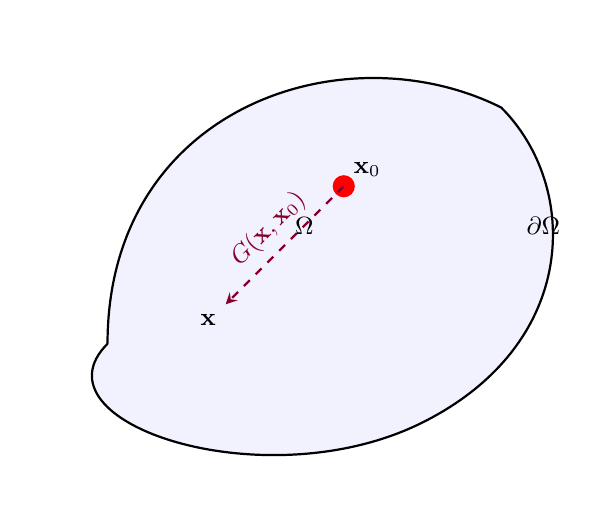
\begin{tikzpicture}[
  pde08region/.style = {thick, fill=blue!8},
  pde08src/.style = {fill=red, circle, inner sep=2pt},
  pde08obs/.style = {fill=blue, circle, inner sep=2pt},
  pde08arr/.style = {->, >=stealth, thick, dashed, purple!70!black},
  pde08lbl/.style = {font=\small}
]
  % 鍖哄煙
  \draw[pde08region, fill=blue!5] (0,0) .. controls (0,3) and (3,4) ..
    (5,3) .. controls (6,2) and (6,0) .. (4,-1) ..
    controls (2,-2) and (-1,-1) .. (0,0);
  \node[pde08lbl] at (2.5,1.5) {$\Omega$};
  % 杈圭晫
  \node[pde08lbl, right] at (5.2,1.5) {$\partial\Omega$};
  % 婧愮偣
  \fill[pde08src] (3,2) circle (4pt);
  \node[pde08lbl, above right] at (3,2) {$\mathbf{x}_0$};
  % 瑙傚療鐐?  \fill[pde08obs] (1.5,0.5) circle (4pt);
  \node[pde08lbl, below left] at (1.5,0.5) {$\mathbf{x}$};
  % 绠ご
  \draw[pde08arr] (3,2) -- (1.5,0.5)
    node[midway, above, font=\small, sloped] {$G(\mathbf{x},\mathbf{x}_0)$};
\end{tikzpicture}
\caption{鏍兼灄鍑芥暟绀烘剰鍥撅細鐐规簮 $\mathbf{x}_0$ 鍒拌瀵熺偣 $\mathbf{x}$ 鐨勫搷搴攠
\end{figure}

%% ============================================================
\section{娉婃澗鏂圭▼鐨勬牸鏋楀嚱鏁皚

鑰冭檻 Poisson 鏂圭▼鐨?Dirichlet 杈瑰€奸棶棰橈細
\begin{equation}
\begin{cases}
  -\Delta u(\mathbf{x}) = f(\mathbf{x}), & \mathbf{x}\in\Omega, \\[4pt]
  u(\mathbf{x}) = g(\mathbf{x}), & \mathbf{x}\in\partial\Omega.
\end{cases}
\label{eq:poisson}
\end{equation}

\begin{myTheorem}{Poisson 鏂圭▼瑙ｇ殑绉垎琛ㄧず}
璁?$G(\mathbf{x},\mathbf{x}_0)$ 鏄?$-\Delta$ 鍦?$\Omega$ 涓婂搴?Dirichlet 杈圭晫鏉′欢鐨勬牸鏋楀嚱鏁帮紝鍗?\[
  \begin{cases}
    -\Delta_{\mathbf{x}} G(\mathbf{x},\mathbf{x}_0)
    = \delta(\mathbf{x}-\mathbf{x}_0), & \mathbf{x}\in\Omega, \\
    G(\mathbf{x},\mathbf{x}_0) = 0, & \mathbf{x}\in\partial\Omega,
  \end{cases}
\]
鍒欓棶棰榽\eqref{eq:poisson} 鐨勮В涓?\[
  u(\mathbf{x}_0) = \int_\Omega G(\mathbf{x},\mathbf{x}_0)\,f(\mathbf{x})\,d\mathbf{x}
  + \oint_{\partial\Omega} g(\mathbf{x})\,
  \frac{\partial G(\mathbf{x},\mathbf{x}_0)}{\partial n_{\mathbf{x}}}\,dS_{\mathbf{x}}.
\]
\end{myTheorem}

\begin{myremark}
娉ㄦ剰鏍兼灄鍑芥暟鍏锋湁瀵圭О鎬э細$G(\mathbf{x},\mathbf{x}_0)=G(\mathbf{x}_0,\mathbf{x})$銆傝繖琚О涓篭textbf{浜掓槗瀹氱悊}锛圧eciprocity Theorem锛夛紝鍏剁墿鐞嗗惈涔夋槸锛氬湪 $\mathbf{x}_0$ 澶勭殑鐐规簮鍦?$\mathbf{x}$ 澶勪骇鐢熺殑鍝嶅簲锛岀瓑浜庡湪 $\mathbf{x}$ 澶勭殑鐐规簮鍦?$\mathbf{x}_0$ 澶勪骇鐢熺殑鍝嶅簲銆?\end{myremark}

瀵逛簬涓夌淮鍏ㄧ┖闂寸殑 Poisson 鏂圭▼锛屾牸鏋楀嚱鏁颁负
\[
  G_0(\mathbf{x},\mathbf{x}_0) = \frac{1}{4\pi|\mathbf{x}-\mathbf{x}_0|}.
\]

瀵逛簬浜岀淮鍏ㄧ┖闂达紝鏍兼灄鍑芥暟涓?\[
  G_0(\mathbf{x},\mathbf{x}_0) = -\frac{1}{2\pi}\ln|\mathbf{x}-\mathbf{x}_0|.
\]

\begin{figure}[htbp]
\centering
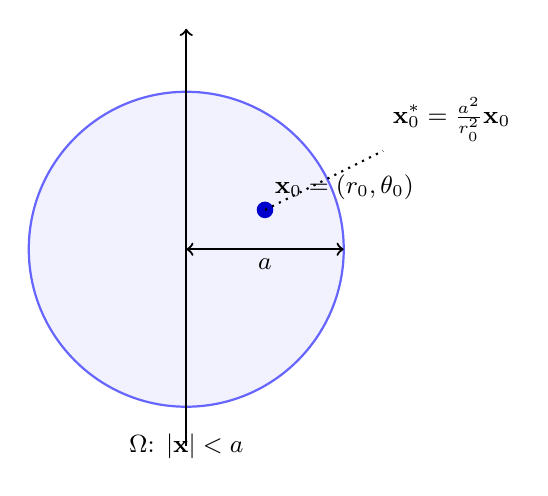
\begin{tikzpicture}[
  pde08sphere/.style = {thick, fill=blue!5, draw=blue!60},
  pde08mirror/.style = {fill=red!20, draw=red!60, dashed},
  pde08lbl/.style = {font=\small}
]
  % 鐞冨煙
  \draw[pde08sphere] (0,0) circle (2cm);
  \node[pde08lbl] at (0,-2.5) {$\Omega$: $|\mathbf{x}|<a$};
  % 鍐呴儴婧愮偣
  \fill[blue!80!black] (1,0.5) circle (3pt);
  \node[pde08lbl, above right] at (1,0.5)
    {$\mathbf{x}_0=(r_0,\theta_0)$};
  % 闀滃儚鐐?  \fill[red!80!black] (2.5,1.25) circle (3pt);
  \node[pde08lbl, above right] at (2.5,1.25)
    {$\mathbf{x}_0^*=\frac{a^2}{r_0^2}\mathbf{x}_0$};
  % 鍗婂緞
  \draw[thick, <->] (0,0) -- (2,0);
  \node[pde08lbl, below] at (1,0) {$a$};
  % 杩炵嚎
  \draw[dotted, thick] (1,0.5) -- (2.5,1.25);
  % 鍧愭爣杞?  \draw[->, thick] (-2.5,0) -- (3.2,0);
  \draw[->, thick] (0,-2.5) -- (0,2.8);
\end{tikzpicture}
\caption{闀滃儚娉曟眰瑙ｇ悆鍩熷唴鐨勬牸鏋楀嚱鏁皚
\end{figure}

\begin{mydefinition}{闀滃儚娉晑
瀵逛簬鍏锋湁绠€鍗曞嚑浣曞舰鐘剁殑鍖哄煙锛屽彲浠ラ€氳繃寮曞叆闀滃儚鐐规簮鏉ユ瀯閫犳牸鏋楀嚱鏁般€傚浜庡崐寰勪负 $a$ 鐨勭悆鍩燂紝鑻ョ湡瀹炴簮鐐瑰湪 $\mathbf{x}_0$锛?|\mathbf{x}_0|<a$锛夛紝鍒欏湪 $\mathbf{x}_0^*=\frac{a^2}{|\mathbf{x}_0|^2}\mathbf{x}_0$ 澶勬斁缃暅鍍忔簮锛屾牸鏋楀嚱鏁颁负
\[
  G(\mathbf{x},\mathbf{x}_0) = \frac{1}{4\pi|\mathbf{x}-\mathbf{x}_0|}
  - \frac{a}{4\pi|\mathbf{x}_0|\,\left|\mathbf{x}-\mathbf{x}_0^*\right|}.
\]
\end{mydefinition}

%% ============================================================
\section{鐑紶瀵兼柟绋嬬殑鏍兼灄鍑芥暟}

鑰冭檻鐑紶瀵兼柟绋嬬殑鍒濆€奸棶棰橈細
\begin{equation}
\begin{cases}
  \dfrac{\partial u}{\partial t} = k\Delta u + f(\mathbf{x},t),
  & \mathbf{x}\in\mathbb{R}^n,\; t>0, \\[6pt]
  u(\mathbf{x},0) = \varphi(\mathbf{x}), & \mathbf{x}\in\mathbb{R}^n.
\end{cases}
\label{eq:heat-green}
\end{equation}

\begin{mydefinition}{鐑紶瀵兼柟绋嬬殑鏍兼灄鍑芥暟}
鐑紶瀵兼柟绋嬬殑鍩烘湰瑙ｏ紙涔熺О鐑牳鎴?Poisson 鏍革級瀹氫箟涓?\[
  G(\mathbf{x},t;\mathbf{x}_0,\tau) = \frac{1}{[4\pi k(t-\tau)]^{n/2}}
  \exp\!\left(-\frac{|\mathbf{x}-\mathbf{x}_0|^2}{4k(t-\tau)}\right),
  \quad t>\tau.
\]
瀹冩弧瓒?\[
  \frac{\partial G}{\partial t} = k\Delta G
  + \delta(\mathbf{x}-\mathbf{x}_0)\,\delta(t-\tau),\quad
  G(\mathbf{x},0;\mathbf{x}_0,\tau) = 0.
\]
\end{mydefinition}

\begin{myTheorem}{鐑紶瀵兼柟绋嬬殑 Duhamel 鍘熺悊}
闂~\eqref{eq:heat-green} 鐨勮В鍙互琛ㄧず涓?\[
  u(\mathbf{x},t) = \int_{\mathbb{R}^n}
  G(\mathbf{x},t;\mathbf{x}_0,0)\,\varphi(\mathbf{x}_0)\,d\mathbf{x}_0
  + \int_0^t\!\!\int_{\mathbb{R}^n}
  G(\mathbf{x},t;\mathbf{x}_0,\tau)\,f(\mathbf{x}_0,\tau)\,
  d\mathbf{x}_0\,d\tau.
\]
鍗宠В = 鍒濆鏉′欢鐨勮础鐚?+ 澶栧姏椤圭殑璐＄尞銆?\end{myTheorem}

\begin{myremark}
Duhamel 鍘熺悊鐨勬€濇兂闈炲父鐩磋锛氬皢澶栧姏 $f(\mathbf{x},t)$ 鐪嬩綔鍦ㄤ笉鍚屾椂鍒?$\tau$ 渚濇鏂藉姞鐨勮剦鍐诧紝姣忎釜鑴夊啿浜х敓鐨勫搷搴旂敱鐑牳缁欏嚭锛屾€诲搷搴斿垯閫氳繃瀵规墍鏈夋椂鍒荤Н鍒嗗緱鍒般€?\end{myremark}

涓嬮潰缁欏嚭涓€涓?Python 绀轰緥锛屽睍绀虹儹鏍哥殑涓夌淮鍙鍖栵細

\begin{lstlisting}[language=Python, caption={涓夌淮鐑牳鐨勫彲瑙嗗寲}]
import numpy as np
import matplotlib.pyplot as plt
from mpl_toolkits.mplot3d import Axes3D

def heat_kernel_2d(x, y, t, k=0.01):
    """浜岀淮鐑牳"""
    return (1.0 / (4 * np.pi * k * t)) * \
           np.exp(-(x**2 + y**2) / (4 * k * t))

# 缃戞牸
N = 200
x = np.linspace(-2, 2, N)
y = np.linspace(-2, 2, N)
X, Y = np.meshgrid(x, y)

fig = plt.figure(figsize=(12, 4))
times = [0.01, 0.05, 0.2]

for i, t in enumerate(times):
    ax = fig.add_subplot(1, 3, i+1, projection='3d')
    Z = heat_kernel_2d(X, Y, t, k=0.01)
    ax.plot_surface(X, Y, Z, cmap='hot', alpha=0.9)
    ax.set_title(f'$t={t}$', fontsize=12)
    ax.set_xlabel('$x$')
    ax.set_ylabel('$y$')
    ax.set_zlabel('$G$')

plt.tight_layout()
plt.show()
\end{lstlisting}

\begin{figure}[htbp]
\centering
\begin{tikzpicture}[
  pde08timeline/.style = {thick, ->, >=stealth},
  pde08pulse/.style = {fill=red!60, circle, inner sep=1.5pt},
  pde08resp/.style = {thick, blue!70!black},
  pde08lbl/.style = {font=\small}
]
  % 鏃堕棿杞?  \draw[pde08timeline] (-0.5,0) -- (12,0) node[right] {$t$};
  % 鑴夊啿鏃跺埢
  \foreach \x/\tau in {2/0, 4.5/1, 7/2, 9.5/3} {
    \draw[pde08pulse] (\x,0) circle (3pt);
    \node[pde08lbl, below] at (\x,-0.3) {$\tau=\tau_{\tau}$};
  }
  % 鍝嶅簲
  \draw[pde08resp] (2,0) .. controls (2,1.5) and (3,1.5) .. (4.5,0);
  \draw[pde08resp] (4.5,0) .. controls (4.5,1.2) and (5.5,1.2) .. (7,0);
  \draw[pde08resp] (7,0) .. controls (7,0.9) and (8,0.9) .. (9.5,0);
  % 鏍囨敞
  \node[pde08lbl, above] at (3.25,1.6) {$G(\cdot,\tau_1)$};
  \node[pde08lbl, above] at (5.75,1.3) {$G(\cdot,\tau_2)$};
  \node[pde08lbl, above] at (8.25,1.0) {$G(\cdot,\tau_3)$};
  % 绉垎绗﹀彿
  \node[pde08lbl, font=\small] at (6,2.5)
    {鎬诲搷搴?$= \int_0^t G(\mathbf{x},t;\mathbf{x}_0,\tau)\,f(\mathbf{x}_0,\tau)\,d\tau$};
\end{tikzpicture}
\caption{Duhamel 鍘熺悊绀烘剰鍥撅細涓嶅悓鏃跺埢鐨勮剦鍐插強鍏跺搷搴攠
\end{figure}

%% ============================================================
\section{娉㈠姩鏂圭▼鐨勬牸鏋楀嚱鏁皚

鑰冭檻涓夌淮娉㈠姩鏂圭▼鐨勫垵鍊奸棶棰橈細
\begin{equation}
\begin{cases}
  \dfrac{\partial^2 u}{\partial t^2} = a^2\Delta u
  + f(\mathbf{x},t), & \mathbf{x}\in\mathbb{R}^3,\; t>0, \\[6pt]
  u(\mathbf{x},0) = \varphi(\mathbf{x}),\quad
  u_t(\mathbf{x},0) = \psi(\mathbf{x}), & \mathbf{x}\in\mathbb{R}^3.
\end{cases}
\label{eq:wave-green}
\end{equation}

\begin{myDefinition}{娉㈠姩鏂圭▼鐨勬牸鏋楀嚱鏁皚
涓夌淮娉㈠姩鏂圭▼鐨勬牸鏋楀嚱鏁颁负
\[
  G(\mathbf{x},t;\mathbf{x}_0,\tau) = \frac{\delta(t-\tau-|\mathbf{x}-\mathbf{x}_0|/a)}
  {4\pi|\mathbf{x}-\mathbf{x}_0|}.
\]
瀹冭〃绀哄湪鏃跺埢 $\tau$銆佷綅缃?$\mathbf{x}_0$ 澶勭殑鍗曚綅鑴夊啿婧愬湪鏃跺埢 $t$銆佷綅缃?$\mathbf{x}$ 澶勪骇鐢熺殑鍝嶅簲銆?\end{mydefinition}

\begin{myTheorem}{涓夌淮娉㈠姩鏂圭▼鐨?Kirchhoff 鍏紡}
闂~\eqref{eq:wave-green} 鐨勮В涓?\begin{align*}
  u(\mathbf{x},t) &= \frac{\partial}{\partial t}
  \left(\frac{1}{4\pi a^2 t}\int_{|\mathbf{x}_0-\mathbf{x}|=at}
  \varphi(\mathbf{x}_0)\,dS_{\mathbf{x}_0}\right) \\
  &\quad + \frac{1}{4\pi a^2 t}\int_{|\mathbf{x}_0-\mathbf{x}|=at}
  \psi(\mathbf{x}_0)\,dS_{\mathbf{x}_0} \\
  &\quad + \int_0^t\!\!\int_{|\mathbf{x}_0-\mathbf{x}|=a(t-\tau)}
  \frac{f(\mathbf{x}_0,\tau)}{4\pi a^2(t-\tau)}\,dS_{\mathbf{x}_0}\,d\tau.
\end{align*}
\end{myTheorem}

\begin{myremark}
娉㈠姩鏂圭▼鐨勮В鏈変竴涓噸瑕佺壒寰佲€斺€擻textbf{Huygens 鍘熺悊}锛氫笁缁存尝鍔ㄦ柟绋嬬殑瑙ｅ湪鏃跺埢 $t$ 鍙緷璧栦簬浠?$\mathbf{x}$ 涓轰腑蹇冦€佸崐寰勪负 $at$ 鐨勭悆闈笂鐨勫垵濮嬫暟鎹€傝繖鎰忓懗鐫€淇″彿浠ユ湁闄愰€熷害 $a$ 浼犳挱锛屼笉浼氱暀涓?灏惧反"銆傝繖涓庣儹浼犲鏂圭▼褰㈡垚椴滄槑瀵规瘮鈥斺€旂儹浼犲鏂圭▼鐨勫奖鍝嶆槸鐬棿浼犻亶鍏ㄧ┖闂寸殑锛堣櫧鐒惰繙澶勭殑褰卞搷鎸囨暟琛板噺锛夈€?\end{myremark}

\begin{figure}[htbp]
\centering
\begin{tikzpicture}[
  pde08wave/.style = {thick, blue!70!black},
  pde08front/.style = {thick, red, dashed},
  pde08lbl/.style = {font=\small}
]
  % 娉㈠墠
  \foreach \r in {1,2,3} {
    \draw[pde08front] (0,0) circle (\r cm);
  }
  % 娉㈠墠鏍囨敞
  \node[pde08lbl, red] at (3.3,0) {$at$};
  \node[pde08lbl, red] at (2.2,0) {$a(t-\Delta t)$};
  \node[pde08lbl, red] at (1.2,0) {$a(t-2\Delta t)$};
  % 涓績
  \fill (0,0) circle (3pt);
  \node[pde08lbl, below right] at (0,0) {$\mathbf{x}_0$};
  % 鍧愭爣杞?  \draw[->, thick] (-3.5,0) -- (4,0) node[right] {$x$};
  \draw[->, thick] (0,-3.5) -- (0,3.8);
  % 鏍囨敞
  \node[pde08lbl] at (0,3.3) {Huygens 鍘熺悊锛氭尝鍓嶄互閫熷害 $a$ 浼犳挱};
\end{tikzpicture}
\caption{娉㈠姩鏂圭▼鐨勬尝鍓嶄紶鎾瓆
\end{figure}

%% ============================================================
\section{鏍兼灄鍑芥暟鐨勭墿鐞嗘剰涔墋

鏍兼灄鍑芥暟鍏锋湁娣卞埢鐨勭墿鐞嗘剰涔夛紝涓嬭〃鎬荤粨浜嗕笉鍚岀被鍨嬫柟绋嬬殑鏍兼灄鍑芥暟鐨勭墿鐞嗗惈涔夛細

\begin{figure}[htbp]
\centering
\begin{tikzpicture}[
  pde07tbl/.style = {matrix of math nodes,
    nodes={draw, minimum width=5cm, minimum height=0.9cm,
           anchor=center, font=\small},
    row sep=0pt, column sep=0pt}
]
  \matrix[pde07tbl] {
    鏂圭▼绫诲瀷 & 鏍兼灄鍑芥暟鐨勭墿鐞嗘剰涔?\\
    \rule{0pt}{8pt} & \rule{0pt}{8pt} \\
    Laplace 鏂圭▼ & 鐐圭數鑽凤紙闈欑數瀛︼級鎴栫偣璐ㄩ噺锛堝紩鍔涳級鐨勫娍 \\
    \rule{0pt}{8pt} & \rule{0pt}{8pt} \\
    鐑紶瀵兼柟绋?& 鐬椂鐐圭儹婧愮殑娓╁害鍝嶅簲 \\
    \rule{0pt}{8pt} & \rule{0pt}{8pt} \\
    娉㈠姩鏂圭▼ & 鑴夊啿鐐规簮浜х敓鐨勬尝 \\
    \rule{0pt}{8pt} & \rule{0pt}{8pt} \\
    Helmholtz 鏂圭▼ & 鍗曢鐐规簮鐨勭ǔ鎬佸搷搴?\\
  };
  \node[font=\small\bfseries, anchor=center]
    at (matrix cs:1-1) {鏂圭▼绫诲瀷};
  \node[font=\small\bfseries, anchor=center]
    at (matrix cs:1-2) {鏍兼灄鍑芥暟鐨勭墿鐞嗘剰涔墋;
\end{tikzpicture}
\caption{涓嶅悓鏂圭▼鐨勬牸鏋楀嚱鏁扮殑鐗╃悊鎰忎箟}
\end{figure}

\begin{myTheorem}{鏍兼灄鍑芥暟鐨勬€ц川}
鏍兼灄鍑芥暟鍏锋湁浠ヤ笅閲嶈鎬ц川锛?\begin{enumerate}
  \item \textbf{瀵圭О鎬锛?G(\mathbf{x},\mathbf{x}_0)=G(\mathbf{x}_0,\mathbf{x})$锛堣嚜浼寸畻瀛愭儏褰級銆?  \item \textbf{濂囧紓鎬锛氬湪 $\mathbf{x}=\mathbf{x}_0$ 澶勫叿鏈夊寮傛€э紝濂囧紓鎬х殑闃朵笌绌洪棿缁存暟鏈夊叧銆?  \item \textbf{闈炶礋鎬锛氬浜?Laplace 鏂圭▼鐨?Dirichlet 鏍兼灄鍑芥暟锛?G(\mathbf{x},\mathbf{x}_0)>0$銆?  \item \textbf{杈圭晫鏉′欢}锛氬湪杈圭晫 $\partial\Omega$ 涓婃弧瓒抽綈娆¤竟鐣屾潯浠躲€?\end{enumerate}
\end{myTheorem}

\begin{myremark}
鏍兼灄鍑芥暟娉曠殑浼樺娍鍦ㄤ簬锛氫竴鏃︽眰鍑轰簡鏍兼灄鍑芥暟锛屽浜庝笉鍚岀殑婧愰」 $f$ 鍜岃竟鐣屾潯浠?$g$锛屽彧闇€鍋氱Н鍒嗚繍绠楀嵆鍙緱鍒拌В锛屼笉闇€瑕侀噸鏂拌В鏂圭▼銆傝繖瀵逛簬闇€瑕佸弽澶嶆眰瑙ｅ悓涓€鍖哄煙涓婁笉鍚屾簮椤圭殑闂灏ゅ叾鏈夌敤銆?\end{myremark}

\begin{lstlisting}[language=Python, caption={鍒╃敤鏍兼灄鍑芥暟鏁板€艰绠楁硦鏉炬柟绋嬬殑瑙]
import numpy as np
import matplotlib.pyplot as plt

def green_function_2d(x, y, x0, y0):
    """浜岀淮 Laplace 鏂圭▼鐨勫熀鏈В"""
    r2 = (x - x0)**2 + (y - y0)**2
    r2 = np.maximum(r2, 1e-12)  # 閬垮厤闄ら浂
    return -np.log(np.sqrt(r2)) / (2 * np.pi)

# 婧愰」 f(x,y) = delta(x,y)锛堢偣婧愬湪鍘熺偣锛?# 鍦ㄥ渾鐩樹笂鐨勬硦鏉炬柟绋?-laplacian u = delta
N = 300
x = np.linspace(-1.5, 1.5, N)
y = np.linspace(-1.5, 1.5, N)
X, Y = np.meshgrid(x, y)

# 鐢ㄧ偣婧愯繎浼?delta 鍑芥暟
x0, y0 = 0.0, 0.0
U = green_function_2d(X, Y, x0, y0)

# 瑁佸壀鍒板渾鐩樺唴
mask = X**2 + Y**2 > 1.0
U[mask] = np.nan

fig, ax = plt.subplots(figsize=(7, 6))
im = ax.contourf(X, Y, U, levels=50, cmap='RdBu_r')
plt.colorbar(im, ax=ax, label='$u$')
circle = plt.Circle((0,0), 1.0, fill=False, color='k', lw=2)
ax.add_patch(circle)
ax.set_aspect('equal')
ax.set_title('娉婃澗鏂圭▼鐨勮В锛堟牸鏋楀嚱鏁版硶锛?)
ax.set_xlabel('$x$')
ax.set_ylabel('$y$')
plt.tight_layout()
plt.show()
\end{lstlisting}

%% ============================================================
\section*{鏈珷灏忕粨}

鏈珷绯荤粺浠嬬粛浜嗘牸鏋楀嚱鏁版硶鐨勫熀鏈悊璁哄拰搴旂敤锛?\begin{itemize}
  \item 鏍兼灄鍑芥暟鏄嚎鎬у井鍒嗙畻瀛愬湪鐐规簮婵€鍔变笅鐨勫搷搴旓紝鏄亸寰垎鏂圭▼鐨勫熀鏈В锛?  \item 鍒╃敤鏍兼灄鍏紡锛屽彲浠ュ皢鍋忓井鍒嗘柟绋嬬殑瑙ｈ〃绀轰负鏍兼灄鍑芥暟涓庢簮椤广€佽竟鐣屾暟鎹殑绉垎锛?  \item 娉婃澗鏂圭▼鐨勬牸鏋楀嚱鏁板彲閫氳繃闀滃儚娉曠瓑鏂规硶鏋勯€狅紱
  \item 鐑紶瀵兼柟绋嬬殑鏍兼灄鍑芥暟锛堢儹鏍革級涓庨珮鏂垎甯冨瘑鍒囩浉鍏筹紱
  \item 娉㈠姩鏂圭▼鐨勬牸鏋楀嚱鏁颁綋鐜颁簡 Huygens 鍘熺悊鈥斺€斾俊鍙蜂互鏈夐檺閫熷害浼犳挱銆?\end{itemize}

%% ============================================================
\section*{缁冧範棰榼

\begin{enumerate}
  \item 姹備簩缁?Laplace 鏂圭▼鍦ㄤ笂鍗婂钩闈?$\{(x,y):y>0\}$ 涓婃弧瓒?Dirichlet 杈圭晫鏉′欢鐨勬牸鏋楀嚱鏁帮紙鎻愮ず锛氬埄鐢ㄩ暅鍍忔硶锛夈€?
  \item 楠岃瘉涓夌淮鐑牳
  \[
    G(\mathbf{x},t) = \frac{1}{(4\pi kt)^{3/2}}e^{-|\mathbf{x}|^2/(4kt)}
  \]
  婊¤冻鐑紶瀵兼柟绋?$G_t = k\Delta G$锛?t>0$锛夈€?
  \item 鍒╃敤 Kirchhoff 鍏紡锛屾眰瑙ｄ笁缁存尝鍔ㄦ柟绋嬪垵鍊奸棶棰橈細
  \[
    u_{tt} = \Delta u,\quad u(\mathbf{x},0)=0,\quad u_t(\mathbf{x},0)=\psi(\mathbf{x}),
  \]
  鍏朵腑 $\psi$ 鍏锋湁鐞冨绉版€с€?
  \item 瑙ｉ噴涓轰粈涔堜簩缁存尝鍔ㄦ柟绋嬩笉婊¤冻 Huygens 鍘熺悊锛屽苟涓庝笁缁存儏褰㈣繘琛屽姣斻€?\end{enumerate}

\chapter{鍙樺垎娉晑

\section*{寮曡█}

鍙樺垎娉曪紙Calculus of Variations锛夋槸鐮旂┒娉涘嚱鏋佸€奸棶棰樼殑鏁板鍒嗘敮锛屽畠鍦ㄦ暟瀛︾墿鐞嗘柟绋嬩腑鏈夌潃骞挎硾鑰屾繁鍒荤殑搴旂敤銆傝澶氱墿鐞嗗畾寰嬪彲浠ヨ〃杩颁负鏌愪釜浣滅敤閲忔硾鍑界殑鏋佸€兼潯浠讹紙鍗虫渶灏忎綔鐢ㄩ噺鍘熺悊锛夛紝鐢辨瀵煎嚭鐨?Euler--Lagrange 鏂圭▼寰€寰€灏辨槸鎻忚堪绯荤粺鐨勫亸寰垎鏂圭▼銆傛澶栵紝鍙樺垎娉曡繕鎻愪緵浜嗘眰瑙ｅ亸寰垎鏂圭▼鐨勮繎浼兼柟娉曪紝濡?Rayleigh--Ritz 鏂规硶鍜屾湁闄愬厓鏂规硶銆?
\begin{myremark}
鍙樺垎娉曠殑鍘嗗彶鍙互杩芥函鍒?Newton銆丒uler 鍜?Lagrange 绛変汉鐨勫伐浣溿€?696 骞?Johann Bernoulli 鎻愬嚭鐨勬渶閫熼檷绾块棶棰橈紙Brachistochrone Problem锛夋槸鍙樺垎娉曠殑缁忓吀璧锋簮涔嬩竴銆傝繘鍏?20 涓栫邯鍚庯紝鍙樺垎娉曚笌鍋忓井鍒嗘柟绋嬬殑鑱旂郴鍙樺緱瓒婃潵瓒婄揣瀵嗭紝鎴愪负鐜颁唬鏁板鐗╃悊鐨勬牳蹇冨伐鍏蜂箣涓€銆?\end{myremark}

%% ============================================================
\section{娉涘嚱涓庡彉鍒唥

\begin{mydefinition}{娉涘嚱}
璁?$D$ 鏄煇涓嚱鏁扮┖闂翠腑鐨勯泦鍚堛€傛槧灏?$J:D\to\mathbb{R}$ 绉颁负涓€涓猏textbf{娉涘嚱}锛團unctional锛夛紝瀹冨皢姣忎釜鍑芥暟 $y(x)$ 鏄犲皠涓轰竴涓疄鏁般€?\end{mydefinition}

\begin{mydefinition}{鍙樺垎}
璁?$y(x)$ 鏄硾鍑?$J[y]$ 鐨勬瀬鍊煎嚱鏁般€傝€冭檻鎵板姩 $y(x)+\varepsilon\,\eta(x)$锛屽叾涓?$\eta(x)$ 鏄弧瓒宠竟鐣屾潯浠剁殑浠绘剰瀹硅鍑芥暟锛?\varepsilon$ 鏄皬鍙傛暟銆傚垯
\[
  \delta J = \frac{d}{d\varepsilon}J[y+\varepsilon\eta]\bigg|_{\varepsilon=0}
  = \int_a^b \left(\frac{\partial F}{\partial y}\eta
  + \frac{\partial F}{\partial y'}\eta'\right)dx
\]
绉颁负娉涘嚱 $J$ 鐨刓textbf{涓€闃跺彉鍒唥锛團irst Variation锛夛紝璁颁负 $\delta J$銆?\end{mydefinition}

鍏稿瀷鐨勬硾鍑藉舰寮忎负
\[
  J[y] = \int_a^b F(x,y,y')\,dx,
\]
鍏朵腑 $F$ 鏄叧浜?$x$銆?y$ 鍜?$y'=dy/dx$ 鐨勫凡鐭ュ嚱鏁般€?
\begin{figure}[htbp]
\centering
\begin{tikzpicture}[
  pde09curve/.style = {thick, blue!70!black},
  pde09pert/.style = {thick, red, dashed},
  pde09envelope/.style = {fill=blue!10, opacity=0.5},
  pde09lbl/.style = {font=\small}
]
  % 鏋佸€兼洸绾?  \draw[pde09curve, domain=0:4, samples=100]
    plot (\x, {0.3*\x + 0.15*\x^2 - 0.02*\x^3});
  \node[pde09lbl, blue!70!black, right] at (4.1,2.5)
    {$y(x)$锛堟瀬鍊兼洸绾匡級};
  % 鎵板姩鏇茬嚎 1
  \draw[pde09pert, domain=0:4, samples=100]
    plot (\x, {0.3*\x + 0.15*\x^2 - 0.02*\x^3
    + 0.15*sin(deg(\x*180/4))});
  \node[pde09lbl, red, right] at (4.1,2.0)
    {$y+\varepsilon\eta_1$};
  % 鎵板姩鏇茬嚎 2
  \draw[pde09pert, domain=0:4, samples=100]
    plot (\x, {0.3*\x + 0.15*\x^2 - 0.02*\x^3
    - 0.12*sin(deg(\x*180/4))});
  \node[pde09lbl, red, right] at (4.1,1.6)
    {$y+\varepsilon\eta_2$};
  % 绔偣
  \fill (0,0) circle (2.5pt);
  \fill (4,2.56) circle (2.5pt);
  \node[pde09lbl, below left] at (0,0) {$a$};
  \node[pde09lbl, below right] at (4,2.56) {$b$};
  % 鍧愭爣杞?  \draw[->, thick] (-0.5,0) -- (5,0) node[right] {$x$};
  \draw[->, thick] (0,-0.5) -- (0,3.5) node[above] {$y$};
\end{tikzpicture}
\caption{鍙樺垎绀烘剰鍥撅細鏋佸€兼洸绾垮強鍏舵壈鍔▆
\end{figure}

%% ============================================================
\section{Euler--Lagrange 鏂圭▼}

\begin{myTheorem}{Euler--Lagrange 鏂圭▼锛堜竴鍏冨嚱鏁版儏褰級}
璁炬硾鍑?\[
  J[y] = \int_a^b F(x,y,y')\,dx
\]
鍦?$y=y(x)$ 澶勫彇鏋佸€硷紝涓?$y(a)=\alpha$锛?y(b)=\beta$锛堝浐瀹氱鐐规潯浠讹級锛屽垯 $y(x)$ 蹇呮弧瓒?Euler--Lagrange 鏂圭▼
\begin{equation}
  \frac{\partial F}{\partial y} - \frac{d}{dx}\frac{\partial F}{\partial y'} = 0.
  \label{eq:euler-lagrange-1d}
\end{equation}
\end{myTheorem}

\begin{proof}
鑰冭檻鎵板姩 $y+\varepsilon\eta$锛屽叾涓?$\eta(a)=\eta(b)=0$銆傚垯
\[
  J[y+\varepsilon\eta] = \int_a^b F(x,y+\varepsilon\eta,y'+\varepsilon\eta')\,dx.
\]
瀵?$\varepsilon$ 姹傚骞朵护 $\varepsilon=0$锛?\[
  \delta J = \int_a^b \left(\frac{\partial F}{\partial y}\eta
  + \frac{\partial F}{\partial y'}\eta'\right)dx = 0.
\]
瀵圭浜岄」鍒嗛儴绉垎锛?\[
  \int_a^b \frac{\partial F}{\partial y'}\eta'\,dx
  = \left[\frac{\partial F}{\partial y'}\eta\right]_a^b
  - \int_a^b \frac{d}{dx}\frac{\partial F}{\partial y'}\eta\,dx.
\]
鐢?$\eta(a)=\eta(b)=0$锛岃竟鐣岄」娑堝け锛屽緱鍒?\[
  \int_a^b \left(\frac{\partial F}{\partial y}
  - \frac{d}{dx}\frac{\partial F}{\partial y'}\right)\eta\,dx = 0.
\]
鐢卞彉鍒嗗熀鏈紩鐞嗭紙$\eta$ 鐨勪换鎰忔€э級锛岃绉嚱鏁板繀椤讳负闆讹紝鍗冲緱~\eqref{eq:euler-lagrange-1d}銆?\end{proof}

\begin{myTheorem}{Euler--Lagrange 鏂圭▼锛堝鍏冨嚱鏁版儏褰級}
璁?$u(x_1,x_2,\dots,x_n)$ 鏄鍏冨嚱鏁帮紝娉涘嚱
\[
  J[u] = \int_\Omega F(x_1,\dots,x_n,u,u_{x_1},\dots,u_{x_n})\,d\mathbf{x}
\]
鐨勬瀬鍊煎嚱鏁版弧瓒?\begin{equation}
  \frac{\partial F}{\partial u}
  - \sum_{i=1}^{n}\frac{\partial}{\partial x_i}\frac{\partial F}{\partial u_{x_i}} = 0.
  \label{eq:euler-lagrange-nd}
\end{equation}
\end{myTheorem}

\begin{myremark}
褰撴硾鍑戒腑鍖呭惈楂橀樁瀵兼暟鏃讹紝濡?\[
  J[y] = \int_a^b F(x,y,y',y'')\,dx,
\]
Euler--Lagrange 鏂圭▼鎺ㄥ箍涓?\[
  \frac{\partial F}{\partial y} - \frac{d}{dx}\frac{\partial F}{\partial y'}
  + \frac{d^2}{dx^2}\frac{\partial F}{\partial y''} = 0.
\]
\end{myremark}

涓嬮潰缁欏嚭涓€涓粡鍏镐緥瀛愨€斺€旀渶閫熼檷绾块棶棰橈細

\begin{figure}[htbp]
\centering
\begin{tikzpicture}[
  pde09brach/.style = {thick, blue!70!black},
  pde09line/.style = {thick, red, dashed},
  pde09lbl/.style = {font=\small}
]
  % 鍧愭爣杞?  \draw[->, thick] (0,0) -- (5.5,0) node[right] {$x$};
  \draw[->, thick] (0,0) -- (0,4.2) node[above, rotate=90] {$y$};
  % 鎽嗙嚎锛堟渶閫熼檷绾胯繎浼硷級
  \draw[pde09brach, domain=0:4.8, samples=200]
    plot (\x, {1.5*(1 - cos(deg(\x*180/4.8)))});
  \node[pde09brach, right] at (5.0, 2.5) {鎽嗙嚎锛堟渶閫熼檷绾匡級};
  % 鐩寸嚎
  \draw[pde09line] (0,0) -- (4.8, 2.5);
  \node[pde09lbl, red] at (3.5, 0.5) {鐩寸嚎};
  % 绔偣
  \fill[red] (0,0) circle (3pt) node[below left] {$A$};
  \fill[red] (4.8, 2.5) circle (3pt) node[right] {$B$};
  % 閲嶅姏鏂瑰悜
  \draw[->, thick, gray] (2.5, 3.5) -- (2.5, 2.8)
    node[midway, right, font=\small] {$g$};
\end{tikzpicture}
\caption{鏈€閫熼檷绾块棶棰橈細璐ㄧ偣浠?$A$ 鍒?$B$ 鐨勬渶蹇笅闄嶈矾寰勪负鎽嗙嚎}
\end{figure}

%% ============================================================
\section{鏉′欢鍙樺垎}

鍦ㄥ疄闄呭簲鐢ㄤ腑锛岀粡甯搁渶瑕佸湪鏌愪簺绾︽潫鏉′欢涓嬫眰娉涘嚱鐨勬瀬鍊笺€?
\begin{mydefinition}{绛夊懆闂}
鍦ㄧ害鏉熸潯浠?\[
  K[y] = \int_a^b G(x,y,y')\,dx = c \quad (\text{甯告暟})
\]
涓嬶紝姹傛硾鍑?$J[y]=\int_a^b F(x,y,y')\,dx$ 鐨勬瀬鍊硷紝绉颁负\textbf{绛夊懆闂}锛圛soperimetric Problem锛夈€?\end{mydefinition}

\begin{myTheorem}{绛夊懆闂鐨?Euler--Lagrange 鏂圭▼}
鍦ㄧ害鏉?$K[y]=c$ 涓嬫眰 $J[y]$ 鐨勬瀬鍊硷紝寮曞叆 Lagrange 涔樺瓙 $\lambda$锛屾瀯閫犺緟鍔╂硾鍑?\[
  \tilde{J}[y] = J[y] + \lambda K[y]
  = \int_a^b \left[F + \lambda G\right]dx,
\]
鍒欐瀬鍊煎嚱鏁版弧瓒?\[
  \frac{\partial \tilde{F}}{\partial y} - \frac{d}{dx}\frac{\partial \tilde{F}}{\partial y'} = 0,
  \quad \tilde{F} = F + \lambda G.
\]
\end{myTheorem}

\begin{myremark}
绾︽潫鏉′欢涓嶄竴瀹氬彧鏄Н鍒嗗舰寮忕殑銆傚湪鍋忓井鍒嗘柟绋嬬殑鍙樺垎闂涓紝甯歌鐨勭害鏉熻繕鍖呮嫭鏂圭▼鏈韩锛堜綔涓虹瓑寮忕害鏉燂級锛屾鏃跺悓鏍峰彲浠ュ紩鍏?Lagrange 涔樺瓙鏉ュ鐞嗐€傝繖鍦ㄦ湁闄愬厓鏂规硶鐨勫急褰㈠紡鎺ㄥ涓粡甯稿嚭鐜般€?\end{myremark}

\begin{figure}[htbp]
\centering
\begin{tikzpicture}[
  pde09circle/.style = {thick, blue!70!black},
  pde09rect/.style = {thick, red!70!black, dashed},
  pde09lbl/.style = {font=\small}
]
  % 绛夊懆闂绀烘剰锛氬浐瀹氬懆闀夸笅闈㈢Н鏈€澶?  % 鍦?  \draw[pde09circle] (0,1.5) circle (1.5cm);
  \node[pde09lbl, blue!70!black] at (0,1.5) {鍦唥;
  \node[pde09lbl, below] at (0,-0.3)
    {鍛ㄩ暱 $=2\pi r$锛岄潰绉?$=\pi r^2$};
  % 姝ｆ柟褰?  \draw[pde09rect] (3.5,0) rectangle (6.5,3);
  \node[pde09lbl, red!70!black] at (5,1.5) {姝ｆ柟褰;
  \node[pde09lbl, below] at (5,-0.3)
    {鍛ㄩ暱 $=4a$锛岄潰绉?$=a^2$};
  % 姣旇緝
  \node[pde09lbl] at (3.25, 3.8)
    {鐩稿悓鍛ㄩ暱 $\Rightarrow$ 鍦嗙殑闈㈢Н鏈€澶;
\end{tikzpicture}
\caption{绛夊懆闂绀轰緥锛氬懆闀垮浐瀹氭椂鍦嗙殑闈㈢Н鏈€澶
\end{figure}

%% ============================================================
\section{鍙樺垎娉曞湪鍋忓井鍒嗘柟绋嬩腑鐨勫簲鐢▆

鍙樺垎娉曚笌鍋忓井鍒嗘柟绋嬩箣闂存湁鐫€娣卞埢鐨勮仈绯汇€傝澶氶噸瑕佺殑鍋忓井鍒嗘柟绋嬮兘鍙互閫氳繃鍙樺垎鍘熺悊瀵煎嚭銆?
\begin{myTheorem}{Dirichlet 鍘熺悊}
Laplace 鏂圭▼鐨?Dirichlet 闂
\[
  \Delta u = 0 \text{ in } \Omega,\quad u = g \text{ on } \partial\Omega
\]
鐨勮В绛変环浜?Dirichlet 娉涘嚱
\[
  J[u] = \frac{1}{2}\int_\Omega |\nabla u|^2\,d\mathbf{x}
\]
鍦ㄦ弧瓒宠竟鐣屾潯浠?$u|_{\partial\Omega}=g$ 鐨勫嚱鏁颁腑鐨勬瀬灏忓€煎嚱鏁般€?\end{myTheorem}

\begin{proof}
璁＄畻 $J[u+\varepsilon\eta]$锛堝叾涓?$\eta|_{\partial\Omega}=0$锛夛細
\[
  J[u+\varepsilon\eta] = J[u] + \varepsilon\int_\Omega\nabla u\cdot\nabla\eta\,d\mathbf{x}
  + \frac{\varepsilon^2}{2}\int_\Omega|\nabla\eta|^2\,d\mathbf{x}.
\]
瀵圭涓€椤瑰埄鐢?Green 绗竴鍏紡锛?\[
  \int_\Omega\nabla u\cdot\nabla\eta\,d\mathbf{x}
  = -\int_\Omega(\Delta u)\eta\,d\mathbf{x}
  + \oint_{\partial\Omega}\frac{\partial u}{\partial n}\eta\,dS.
\]
鐢?$\eta|_{\partial\Omega}=0$锛岃竟鐣岄」娑堝け銆傛晠
\[
  \delta J = -\int_\Omega(\Delta u)\eta\,d\mathbf{x}.
\]
浠?$\delta J=0$ 瀵规墍鏈?$\eta$ 鎴愮珛锛屽嵆寰?$\Delta u=0$銆?\end{proof}

\begin{myremark}
Dirichlet 鍘熺悊鐨勭墿鐞嗘剰涔夋槸锛氬湪婊¤冻缁欏畾杈圭晫鏉′欢鐨勬墍鏈夋俯搴﹀垎甯冧腑锛岀儹骞宠　鎬佸搴旂殑娓╁害鍒嗗竷浣挎俯搴︽搴︾殑鎬昏兘閲忥紙Dirichlet 鑳介噺锛夋渶灏忋€?\end{myremark}

\begin{mydefinition}{寮卞舰寮弣
璁?$u$ 鏄?PDE 鐨勭粡鍏歌В锛堝厜婊戯級锛屽皢鍏朵箻浠ユ祴璇曞嚱鏁?$v$ 骞跺湪鍖哄煙 $\Omega$ 涓婄Н鍒嗭紝鍒╃敤鍒嗛儴绉垎闄嶄綆瀵兼暟闃舵暟锛屽緱鍒扮殑绉垎褰㈠紡绉颁负鍘熸柟绋嬬殑\textbf{寮卞舰寮弣锛圵eak Formulation锛夈€?
渚嬪锛孭oisson 鏂圭▼ $-\Delta u = f$ 鐨勫急褰㈠紡涓猴細姹?$u\in H^1(\Omega)$ 浣垮緱
\[
  \int_\Omega \nabla u\cdot\nabla v\,d\mathbf{x}
  = \int_\Omega f\,v\,d\mathbf{x},\quad \forall v\in H_0^1(\Omega).
\]
\end{mydefinition}

\begin{figure}[htbp]
\centering
\begin{tikzpicture}[
  pde09flow/.style = {rectangle, draw, minimum width=3.2cm,
    minimum height=0.8cm, text centered, font=\small},
  pde09arr/.style = {->, >=stealth, thick}
]
  \node[pde09flow] (A) at (0,0)   {PDE锛堝己褰㈠紡锛墋;
  \node[pde09flow] (B) at (0,-1.5) {鍙樺垎鍘熺悊锛堟渶灏忎綔鐢ㄩ噺锛墋;
  \node[pde09flow] (C) at (0,-3.0) {寮卞舰寮忥紙绉垎褰㈠紡锛墋;
  \node[pde09flow] (D) at (0,-4.5) {鏈夐檺鍏冪鏁;
  \node[pde09flow] (E) at (0,-6.0) {绾挎€ф柟绋嬬粍姹傝В};

  \draw[pde09arr] (A) -- (B);
  \draw[pde09arr] (B) -- (C);
  \draw[pde09arr] (C) -- (D);
  \draw[pde09arr] (D) -- (E);
\end{tikzpicture}
\caption{浠?PDE 鍒版暟鍊兼眰瑙ｇ殑娴佺▼}
\end{figure}

%% ============================================================
\section{Rayleigh--Ritz 鏂规硶}

\begin{mydefinition}{Rayleigh--Ritz 鏂规硶}
Rayleigh--Ritz 鏂规硶鏄竴绉嶅熀浜庡彉鍒嗗師鐞嗙殑杩戜技姹傝В鏂规硶銆傚叾鍩烘湰鎬濇兂鏄細灏嗘硾鍑界殑鏋佸€兼悳绱㈤檺鍒跺湪涓€涓湁闄愮淮瀛愮┖闂翠腑锛屼粠鑰屽皢鏃犵┓缁寸殑鍙樺垎闂鍖栦负鏈夐檺缁寸殑鏈€浼樺寲闂銆?\end{mydefinition}

鍏蜂綋姝ラ濡備笅锛?\begin{enumerate}
  \item 閫夊彇涓€缁勮瘯鎺㈠嚱鏁?$\{\phi_1,\phi_2,\dots,\phi_N\}$锛屾瀯閫犺繎浼艰В
  \[
    u_N(x) = \sum_{k=1}^{N} c_k\,\phi_k(x).
  \]
  \item 灏?$u_N$ 浠ｅ叆娉涘嚱 $J$锛屽緱鍒板叧浜庣郴鏁?$c_1,\dots,c_N$ 鐨勫嚱鏁?  \[
    J(c_1,\dots,c_N) = J\!\left[\sum_{k=1}^{N}c_k\phi_k\right].
  \]
  \item 浠?$\frac{\partial J}{\partial c_k}=0$锛?k=1,\dots,N$锛夛紝寰楀埌鍏充簬 $c_k$ 鐨勭嚎鎬ф柟绋嬬粍銆?  \item 姹傝В璇ユ柟绋嬬粍锛屽緱鍒拌繎浼艰В $u_N$銆?\end{enumerate}

\begin{myTheorem}{Rayleigh--Ritz 鏂规硶鐨勬敹鏁涙€
璁?$J$ 鏄湁涓嬬晫鐨勪弗鏍煎嚫娉涘嚱锛?\{\phi_k\}$ 鏄畬澶囧熀锛屽垯褰?$N\to\infty$ 鏃讹紝Rayleigh--Ritz 杩戜技瑙?$u_N$ 涓€鑷存敹鏁涘埌鐪熸鐨勬瀬灏忓€煎嚱鏁?$u$锛?\[
  J[u_N] \to J[u],\quad \|u_N-u\|\to 0.
\]
\end{myTheorem}

\begin{myremark}
Rayleigh--Ritz 鏂规硶鏄湁闄愬厓鏂规硶锛團inite Element Method, FEM锛夌殑鐞嗚鍩虹銆傛湁闄愬厓鏂规硶鍙互鐪嬩綔鏄?Rayleigh--Ritz 鏂规硶鐨勪竴绉嶇壒娈婂疄鐜扳€斺€斿畠浣跨敤鍒嗙墖澶氶」寮忎綔涓鸿瘯鎺㈠嚱鏁板熀搴曪紝鍦ㄥ伐绋嬪拰绉戝璁＄畻涓湁鏋佷负骞挎硾鐨勫簲鐢ㄣ€?\end{myremark}

涓嬮潰缁欏嚭涓€涓?Python 绀轰緥锛屽睍绀?Rayleigh--Ritz 鏂规硶姹傝В绠€鏀闂锛?
\begin{lstlisting}[language=Python, caption={Rayleigh--Ritz 鏂规硶姹傝В绠€鏀鐨勭壒寰佸€奸棶棰榼]
import numpy as np
import matplotlib.pyplot as plt

# 绠€鏀鐗瑰緛鍊奸棶棰? u'''' = lambda*u, u(0)=u(1)=u''(0)=u''(1)=0
# 绮剧‘鐗瑰緛鍊? lambda_n = (n*pi)^4, 鐗瑰緛鍑芥暟: sin(n*pi*x)

# Rayleigh--Ritz: 鍙栬瘯鎺㈠嚱鏁?phi_k = sin(k*pi*x), k=1,...,N
# 娉涘嚱: J[u] = int(u''^2 dx) / int(u^2 dx)
# 鍦ㄥ熀搴?{sin(k*pi*x)} 涓? 鍒氬害鐭╅樀鍜岃川閲忕煩闃垫槸瀵硅鐨?
N = 5  # 鍩哄嚱鏁版暟閲?x = np.linspace(0, 1, 500)

# 绮剧‘鐗瑰緛鍊煎拰鐗瑰緛鍑芥暟
exact_eigenvalues = [(n * np.pi)**4 for n in range(1, N+1)]
exact_eigenfunctions = [np.sin(n * np.pi * x) for n in range(1, N+1)]

# Rayleigh--Ritz 杩戜技锛堝湪姝ょ壒渚嬩腑绮剧‘锛?rr_eigenvalues = exact_eigenvalues
rr_eigenfunctions = exact_eigenfunctions

# 缁樺浘锛氬墠3涓壒寰佸嚱鏁?fig, axes = plt.subplots(1, 3, figsize=(12, 3.5))
for i in range(3):
    axes[i].plot(x, rr_eigenfunctions[i], 'b-', linewidth=2)
    axes[i].set_title(f'$\\phi_{i+1}(x)$, $\\lambda={rr_eigenvalues[i]:.1f}$')
    axes[i].set_xlabel('$x$')
    axes[i].grid(True, alpha=0.3)
    axes[i].axhline(y=0, color='k', linewidth=0.5)

plt.suptitle('Rayleigh--Ritz 鏂规硶锛氱畝鏀鐨勭壒寰佸嚱鏁?, fontsize=13)
plt.tight_layout()
plt.show()
\end{lstlisting}

\begin{figure}[htbp]
\centering
\begin{tikzpicture}[
  pde09beam/.style = {thick, draw=black!70},
  pde09support/.style = {thick, draw=black!70, fill=gray!30},
  pde09mode/.style = {thick, blue!70!black},
  pde09lbl/.style = {font=\small}
]
  % 姊?  \draw[pde09beam] (0,1) -- (8,1);
  % 绠€鏀紙涓夎褰級
  \draw[pde09support] (-0.3,1) -- (0.3,1) -- (0,0.5) -- cycle;
  \draw[pde09support] (7.7,1) -- (8.3,1) -- (8,0.5) -- cycle;
  % 绗竴妯℃€?  \draw[pde09mode, domain=0:8, samples=100, shift={(0,2)}]
    plot (\x, {0.5*sin(deg(pi*\x/8))});
  \node[pde09lbl] at (9, 2.5) {$\sin(\pi x/l)$};
  % 绗簩妯℃€?  \draw[pde09mode, domain=0:8, samples=100, shift={(0,4)}]
    plot (\x, {0.5*sin(deg(2*pi*\x/8))});
  \node[pde09lbl] at (9, 4.5) {$\sin(2\pi x/l)$};
  % 绗笁妯℃€?  \draw[pde09mode, domain=0:8, samples=100, shift={(0,6)}]
    plot (\x, {0.5*sin(deg(3*pi*\x/8))});
  \node[pde09lbl] at (9, 6.5) {$\sin(3\pi x/l)$};
  % 鏍囨敞
  \node[pde09lbl] at (4, 0.3) {绠€鏀};
\end{tikzpicture}
\caption{绠€鏀鐨勫墠涓夐樁妯℃€亇
\end{figure}

%% ============================================================
\section*{鏈珷灏忕粨}

鏈珷绯荤粺浠嬬粛浜嗗彉鍒嗘硶鐨勫熀鏈悊璁哄強鍏跺湪鍋忓井鍒嗘柟绋嬩腑鐨勫簲鐢細
\begin{itemize}
  \item 娉涘嚱鏄嚱鏁扮殑鍑芥暟锛屽彉鍒嗘硶鐮旂┒娉涘嚱鏋佸€肩殑蹇呰鏉′欢锛?  \item Euler--Lagrange 鏂圭▼鏄彉鍒嗛棶棰樼殑鍩烘湰鏂圭▼锛屽畠灏嗘硾鍑芥瀬鍊奸棶棰樺寲涓哄井鍒嗘柟绋嬮棶棰橈紱
  \item 绛夊懆闂閫氳繃 Lagrange 涔樺瓙娉曞鐞嗙害鏉熸潯浠讹紱
  \item 璁稿閲嶈鐨勫亸寰垎鏂圭▼锛堝 Laplace 鏂圭▼銆丳oisson 鏂圭▼锛夐兘鏈夊彉鍒嗙粨鏋勶紱
  \item Rayleigh--Ritz 鏂规硶灏嗘棤绌风淮鍙樺垎闂鍖栦负鏈夐檺缁翠唬鏁伴棶棰橈紝鏄湁闄愬厓鏂规硶鐨勭悊璁哄熀纭€銆?\end{itemize}

%% ============================================================
\section*{缁冧範棰榼

\begin{enumerate}
  \item 姹傛硾鍑?  \[
    J[y] = \int_0^1 (y'^2 + y^2 + 2xy)\,dx,\quad y(0)=0,\; y(1)=1
  \]
  鐨勬瀬鍊煎嚱鏁般€?
  \item 鍦ㄧ害鏉?$\int_0^1 y^2\,dx=1$ 涓嬶紝姹傛硾鍑?  \[
    J[y] = \int_0^1 y'^2\,dx,\quad y(0)=y(1)=0
  \]
  鐨勬瀬灏忓€煎嚱鏁板拰鏋佸皬鍊硷紙鎻愮ず锛氳繖鏄壒寰佸€奸棶棰橈級銆?
  \item 鍒╃敤 Dirichlet 鍘熺悊锛岃瘉鏄?Laplace 鏂圭▼ Dirichlet 闂瑙ｇ殑鍞竴鎬с€?
  \item 鐢?Rayleigh--Ritz 鏂规硶锛屽彇涓や釜璇曟帰鍑芥暟锛岃繎浼兼眰瑙ｆ硾鍑?  \[
    J[y] = \int_0^1 (y'^2 - y^2 - 2xy)\,dx,\quad y(0)=y(1)=0
  \]
  鐨勬瀬灏忓€煎嚱鏁般€?\end{enumerate}

\chapter{璐濆灏斿嚱鏁皚

\section*{寮曡█}

璐濆灏斿嚱鏁帮紙Bessel Functions锛夋槸涓€绫婚潪甯搁噸瑕佺殑鐗规畩鍑芥暟锛屽湪鐗╃悊瀛﹀拰宸ョ▼瀛︿腑鏈夌潃骞挎硾鐨勫簲鐢ㄣ€傚綋鎴戜滑鍦ㄥ渾鏌卞潗鏍囩郴鎴栫悆鍧愭爣绯讳腑姹傝В鍋忓井鍒嗘柟绋嬫椂锛岃礉濉炲皵鍑芥暟鍑犱箮涓嶅彲閬垮厤鍦板嚭鐜般€備緥濡傦紝鍦嗗舰鑶滅殑鎸姩闂銆佸渾鏌变綋鍐呯殑鐑紶瀵奸棶棰樹互鍙婄數纾佹尝鍦ㄥ渾褰㈡尝瀵间腑鐨勪紶鎾棶棰樼瓑锛岄兘浼氭秹鍙婅礉濉炲皵鍑芥暟銆?
璐濆灏斿嚱鏁版渶鏃╃敱寰峰浗鏁板瀹?Friedrich Bessel 鍦?1824 骞寸爺绌惰鏄熻繍鍔ㄦ椂绯荤粺寮曞叆锛屾鍚庝互浠栧懡鍚嶃€備簨瀹炰笂锛岃礉濉炲皵鍑芥暟涔熸槸鏌愪簺浜岄樁绾挎€у父寰垎鏂圭▼鐨勮В锛岃繖绫绘柟绋嬬О涓鸿礉濉炲皵鏂圭▼銆傛湰绔犲皢浠庤礉濉炲皵鏂圭▼鐨勬帹瀵煎嚭鍙戯紝绯荤粺浠嬬粛绗竴绫诲拰绗簩绫昏礉濉炲皵鍑芥暟鐨勫畾涔夈€佹€ц川鍜屽簲鐢ㄣ€?
\begin{myremark}
璐濆灏斿嚱鏁扮殑鍘嗗彶鍙互杩芥函鍒?18 涓栫邯銆侲uler 鍦ㄧ爺绌堕紦鑶滄尟鍔ㄦ椂灏辨秹鍙婁簡绫讳技鐨勯棶棰樸€侱aniel Bernoulli 鍜?Euler 鍦ㄧ爺绌跺鸡鎸姩闂鏃朵篃鐢ㄥ埌浜嗙浉鍏崇骇鏁板睍寮€銆侭essel 绯荤粺鍖栧湴鐮旂┒浜嗚繖绫诲嚱鏁扮殑鎬ц川锛屽苟寤虹珛浜嗗畬鏁寸殑鐞嗚浣撶郴銆?\end{myremark}

%% ============================================================
\section{璐濆灏旀柟绋嬬殑鎺ㄥ}

\begin{mydefinition}{璐濆灏旀柟绋媫
鍙傛暟涓?$\nu$锛?\nu \geq 0$锛夌殑\textbf{璐濆灏旀柟绋媫锛圔essel's Equation锛夋槸鎸囧涓嬩簩闃剁嚎鎬у父寰垎鏂圭▼锛?\begin{equation}
  x^2 y'' + x y' + (x^2 - \nu^2) y = 0,
  \label{eq:bessel}
\end{equation}
鍏朵腑 $y=y(x)$ 鏄湭鐭ュ嚱鏁帮紝$\nu$ 绉颁负璐濆灏斿嚱鏁扮殑\textbf{闃秨锛坥rder锛夈€?\end{mydefinition}

璐濆灏旀柟绋嬪彲浠ラ€氳繃鍦ㄦ瀬鍧愭爣鎴栨煴鍧愭爣涓嬪垎绂诲彉閲忔潵寰楀埌銆備笅闈互浜岀淮鍦嗗舰鑶滄尟鍔ㄤ负渚嬭繘琛屾帹瀵笺€?
\begin{myexample}{鍦嗗舰鑶滄尟鍔ㄧ殑鍒嗙鍙橀噺}
鑰冭檻鍦嗗舰鑶滅殑鑷敱鎸姩闂銆傚湪鏋佸潗鏍?$(r,\theta)$ 涓嬶紝浜岀淮娉㈠姩鏂圭▼涓?\[
  \frac{\partial^2 u}{\partial t^2} = c^2 \left(\frac{\partial^2 u}{\partial r^2}
  + \frac{1}{r}\frac{\partial u}{\partial r}
  + \frac{1}{r^2}\frac{\partial^2 u}{\partial \theta^2}\right).
\]
璁?$u(r,\theta,t) = R(r)\Theta(\theta)T(t)$锛屼唬鍏ユ柟绋嬪苟鍒嗙鍙橀噺銆傚浜?$R(r)$锛屽緱鍒?\[
  r^2 R'' + r R' + (\lambda^2 r^2 - n^2) R = 0,
\]
鍏朵腑 $n$ 鏄暣鏁帮紝$\lambda$ 鏄垎绂诲父鏁般€備护 $x = \lambda r$锛屽垯
\begin{equation}
  x^2 R'' + x R' + (x^2 - n^2) R = 0,
  \label{eq:bessel-from-drum}
\end{equation}
杩欐鏄樁鏁?$\nu = n$ 鐨勮礉濉炲皵鏂圭▼銆?\end{myexample}

\begin{figure}[htbp]
\centering
\begin{tikzpicture}[
  pde10membrane/.style = {thick, draw=blue!70!black, fill=blue!10},
  pde10axis/.style = {->, thick},
  pde10lbl/.style = {font=\small},
  pde10node/.style = {circle, fill=red!70!black, inner sep=1.5pt}
]
  % 鍦嗗舰鑶?  \draw[pde10membrane] (0,0) circle (3cm);
  \draw[dashed, gray] (0,0) -- (3,0) node[midway, below, pde10lbl] {$a$};
  % 鍧愭爣杞?  \draw[pde10axis] (-3.8,0) -- (3.8,0) node[right, pde10lbl] {$x$};
  \draw[pde10axis] (0,-3.8) -- (0,3.8) node[above, pde10lbl] {$y$};
  % 鑺傜偣鍦?  \draw[dashed, red!70!black] (0,0) circle (1.2cm);
  \draw[dashed, red!70!black] (0,0) circle (2.3cm);
  \node[pde10lbl, red!70!black] at (2.8, 1.8) {鑺傜嚎};
  % 鏍囨敞
  \node[pde10lbl] at (0, -4.2) {鍦嗗舰鑶滐細鑺傜嚎涓哄悓蹇冨渾鍜屽緞鍚戠嚎};
\end{tikzpicture}
\caption{鍦嗗舰鑶滄尟鍔ㄧ殑鑺傜嚎绀烘剰}
\end{figure}

璐濆灏旀柟绋媬\eqref{eq:bessel} 鍦ㄦ鍒欏鐐?$x=0$ 澶勬湁涓や釜绾挎€х嫭绔嬭В銆傚綋 $\nu$ 涓嶆槸鏁存暟鏃讹紝涓や釜瑙ｅ垎鍒涓?$J_\nu(x)$ 鍜?$J_{-\nu(x)}$锛涘綋 $\nu$ 涓烘暣鏁版椂锛?J_n(x)$ 鍜?$J_{-n}(x)$ 绾挎€х浉鍏筹紝闇€瑕佸紩鍏ョ浜岀被璐濆灏斿嚱鏁?$Y_n(x)$銆?
%% ============================================================
\section{绗竴绫昏礉濉炲皵鍑芥暟}

\begin{mydefinition}{绗竴绫昏礉濉炲皵鍑芥暟}
闃舵暟涓?$\nu$ 鐨刓textbf{绗竴绫昏礉濉炲皵鍑芥暟}锛圔essel Function of the First Kind锛夊畾涔変负
\begin{equation}
  J_\nu(x) = \sum_{m=0}^{\infty} \frac{(-1)^m}{m!\,\Gamma(m+\nu+1)}
  \left(\frac{x}{2}\right)^{2m+\nu},
  \label{eq:bessel-J}
\end{equation}
鍏朵腑 $\Gamma(\cdot)$ 鏄?Gamma 鍑芥暟銆傚綋 $\nu = n$锛堥潪璐熸暣鏁帮級鏃讹紝
\[
  J_n(x) = \sum_{m=0}^{\infty} \frac{(-1)^m}{m!\,(m+n)!}
  \left(\frac{x}{2}\right)^{2m+n}.
\]
\end{mydefinition}

绗竴绫昏礉濉炲皵鍑芥暟鍏锋湁浠ヤ笅閲嶈鎬ц川锛?
\begin{myTheorem}{绗竴绫昏礉濉炲皵鍑芥暟鐨勫熀鏈€ц川}
璁?$J_\nu(x)$ 涓虹涓€绫昏礉濉炲皵鍑芥暟锛屽垯锛?\begin{enumerate}
  \item \textbf{寰垎閫掓帹鍏崇郴}锛?  \[
    \frac{d}{dx}\left[x^\nu J_\nu(x)\right] = x^\nu J_{\nu-1}(x),
    \qquad
    \frac{d}{dx}\left[x^{-\nu} J_\nu(x)\right] = -x^{-\nu} J_{\nu+1}(x).
  \]
  \item \textbf{鏁存暟闃堕€掓帹鍏崇郴}锛?  \[
    J_{n-1}(x) + J_{n+1}(x) = \frac{2n}{x} J_n(x),
    \qquad
    J_{n-1}(x) - J_{n+1}(x) = 2 J_n'(x).
  \]
  \item \textbf{姝ｄ氦鎬锛氬浜?$\alpha_{np}$ 鍜?$\alpha_{nq}$ 鏄?$J_n(x)$ 鐨勪袱涓笉鍚屾闆剁偣锛?  \[
    \int_0^1 J_n(\alpha_{np}\,r)\,J_n(\alpha_{nq})\,r\,dr = 0
    \quad (p \neq q).
  \]
  \item \textbf{妯￠暱}锛?  \[
    \int_0^1 J_n^2(\alpha_{np}\,r)\,r\,dr
    = \frac{1}{2}\left[J_{n+1}(\alpha_{np})\right]^2.
  \]
\end{enumerate}
\end{myTheorem}

\begin{proof}[姝ｄ氦鎬х殑璇佹槑]
璁?$R_p = J_n(\alpha_{np}\,r)$ 鍜?$R_q = J_n(\alpha_{nq}\,r)$锛屽垎鍒弧瓒?\[
  (rR_p')' + \left(\alpha_{np}^2 r - \frac{n^2}{r}\right) R_p = 0,
  \quad
  (rR_q')' + \left(\alpha_{nq}^2 r - \frac{n^2}{r}\right) R_q = 0.
\]
绗竴寮忎箻浠?$R_q$锛岀浜屽紡涔樹互 $R_p$锛岀浉鍑忓悗鍦?$[0,1]$ 涓婄Н鍒嗭紝鍒╃敤杈圭晫鏉′欢 $R_p(1)=R_q(1)=0$ 鍗冲彲寰楀埌姝ｄ氦鎬с€?\end{proof}

\begin{figure}[htbp]
\centering
\begin{tikzpicture}[
  pde10bessel0/.style = {thick, blue!70!black},
  pde10bessel1/.style = {thick, red!70!black},
  pde10bessel2/.style = {thick, green!50!black},
  pde10axis/.style = {->, thick, gray},
  pde10grid/.style = {gray!30, very thin},
  pde10lbl/.style = {font=\small}
]
  % 鍧愭爣杞?  \draw[pde10axis] (-0.5,0) -- (14,0) node[right, pde10lbl] {$x$};
  \draw[pde10axis] (0,-0.7) -- (0,1.2) node[above, pde10lbl] {$J_n(x)$};
  % 缃戞牸绾?  \foreach \y in {-0.5,0.5,1.0} {
    \draw[pde10grid] (-0.5,\y) -- (14,\y);
  }
  \foreach \x in {2,4,6,8,10,12} {
    \draw[pde10grid] (\x,-0.7) -- (\x,1.2);
  }
  % J_0(x)
  \draw[pde10bessel0, domain=0:13.5, samples=300]
    plot (\x, {0.8*besselJ(0,\x)});
  \node[pde10bessel0, right, pde10lbl] at (13.7, 0.6) {$J_0(x)$};
  % J_1(x)
  \draw[pde10bessel1, domain=0:13.5, samples=300]
    plot (\x, {0.8*besselJ(1,\x)});
  \node[pde10bessel1, right, pde10lbl] at (13.7, 0.2) {$J_1(x)$};
  % J_2(x)
  \draw[pde10bessel2, domain=0:13.5, samples=300]
    plot (\x, {0.8*besselJ(2,\x)});
  \node[pde10bessel2, right, pde10lbl] at (13.7, -0.2) {$J_2(x)$};
  % 闆剁偣鏍囨敞
  \foreach \z in {2.405, 5.520, 8.654} {
    \draw[dashed, gray] (\z, 0.75) -- (\z, -0.05);
  }
\end{tikzpicture}
\caption{鍓嶄笁涓涓€绫昏礉濉炲皵鍑芥暟 $J_0(x)$銆?J_1(x)$銆?J_2(x)$ 鐨勫浘鍍弣
\end{figure}

\begin{myremark}
浠庡浘涓彲浠ョ湅鍑猴紝$J_n(x)$ 鍦?$x=0$ 澶勭殑鍊硷細$J_0(0)=1$锛?J_n(0)=0$锛?n \geq 1$锛夈€傞殢鐫€ $x$ 澧炲ぇ锛?J_n(x)$ 鍛堢幇琛板噺鎸崱鐨勭壒寰侊紝鎸箙浠?$\sim \sqrt{2/(\pi x)}$ 鐨勯€熷害琛板噺銆?\end{myremark}

%% ============================================================
\section{绗簩绫昏礉濉炲皵鍑芥暟}

褰?$\nu = n$ 涓烘暣鏁版椂锛?J_n(x)$ 鍜?$J_{-n}(x)$ 涓嶅啀绾挎€х嫭绔嬶紙鍥犱负 $J_{-n}(x) = (-1)^n J_n(x)$锛夈€傛鏃堕渶瑕佸紩鍏ョ浜岀被璐濆灏斿嚱鏁般€?
\begin{mydefinition}{绗簩绫昏礉濉炲皵鍑芥暟}
闃舵暟涓?$\nu$ 鐨刓textbf{绗簩绫昏礉濉炲皵鍑芥暟}锛圔essel Function of the Second Kind锛夛紝涔熺О涓?Neumann 鍑芥暟鎴?Weber 鍑芥暟锛屽畾涔変负
\begin{equation}
  Y_\nu(x) = \frac{J_\nu(x)\cos(\nu\pi) - J_{-\nu}(x)}{\sin(\nu\pi)},
  \label{eq:bessel-Y}
\end{equation}
褰?$\nu = n$锛堟暣鏁帮級鏃讹紝鍙栨瀬闄?\[
  Y_n(x) = \lim_{\nu \to n} \frac{J_\nu(x)\cos(\nu\pi) - J_{-\nu}(x)}{\sin(\nu\pi)}.
\]
\end{mydefinition}

\begin{myTheorem}{绗簩绫昏礉濉炲皵鍑芥暟鐨勬€ц川}
\begin{enumerate}
  \item $Y_\nu(x)$ 涔熸槸璐濆灏旀柟绋媬\eqref{eq:bessel} 鐨勮В锛?  \item $J_\nu(x)$ 鍜?$Y_\nu(x)$ 鏋勬垚璐濆灏旀柟绋嬬殑涓や釜绾挎€х嫭绔嬭В锛?  \item $Y_n(x)$ 鍦?$x=0$ 澶勬湁濂囧紓鎬э細$Y_n(x) \sim \frac{2}{\pi}\ln\frac{x}{2}$锛堝綋 $n=0$锛夋垨 $Y_n(x) \sim -\frac{(n-1)!}{\pi}\left(\frac{2}{x}\right)^n$锛堝綋 $n \geq 1$锛夛紱
  \item $Y_n(x)$ 鍚屾牱婊¤冻 $J_n(x)$ 鐨勬墍鏈夐€掓帹鍏崇郴銆?\end{enumerate}
\end{myTheorem}

\begin{myremark}
鐢变簬 $Y_n(x)$ 鍦ㄥ師鐐瑰彂鏁ｏ紝鍦ㄥ鐞嗗寘鍚?$r=0$ 鐨勫渾鏌卞尯鍩熷唴鐨勯棶棰橈紙濡傚渾鏌卞唴鐑紶瀵硷級鏃讹紝$Y_n(x)$ 鐨勭郴鏁板繀椤讳负闆躲€傚彧鏈夊湪鐜舰鍖哄煙锛?r \geq r_0 > 0$锛夋垨澶栭儴鍖哄煙锛?r \geq R$锛夌殑闂涓紝$Y_n(x)$ 鎵嶄細鍑虹幇銆?\end{myremark}

璐濆灏旀柟绋嬬殑閫氳В鍙互鍐欎负
\[
  y(x) = A\,J_\nu(x) + B\,Y_\nu(x),
\]
鍏朵腑 $A$銆?B$ 鐢辫竟鐣屾潯浠剁‘瀹氥€?
%% ============================================================
\section{璐濆灏斿嚱鏁扮殑鎬ц川}

\begin{myTheorem}{璐濆灏斿嚱鏁扮殑闆剁偣}
\begin{enumerate}
  \item $J_n(x)$ 鏈夋棤绌峰涓闆剁偣锛岃涓?$\alpha_{n1} < \alpha_{n2} < \cdots$锛屼笖鐩搁偦闆剁偣涔嬮棿鐨勯棿璺濊秼杩戜簬 $\pi$锛?  \item 瀵逛簬涓嶅悓鐨?$n$锛?J_n(x)$ 鍜?$J_{n+1}(x)$ 鐨勬闆剁偣鏄氦閿欐帓鍒楃殑锛?  \item $J_0(x)$ 鐨勭涓€涓闆剁偣涓?$\alpha_{01} \approx 2.4048$锛?J_1(x)$ 鐨勭涓€涓闆剁偣涓?$\alpha_{11} \approx 3.8317$銆?\end{enumerate}
\end{myTheorem}

璐濆灏斿嚱鏁扮殑娓愯繎灞曞紑锛?x \to \infty$锛変负锛?\[
  J_\nu(x) \sim \sqrt{\frac{2}{\pi x}} \cos\left(x - \frac{\nu\pi}{2} - \frac{\pi}{4}\right),
  \quad x \to \infty.
\]
杩欒鏄?$J_n(x)$ 鍦ㄨ繙澶勮繎浼间簬琛板噺鐨勪綑寮﹀嚱鏁般€?
\begin{mydefinition}{璐濆灏斿嚱鏁扮殑姝ｄ氦瀹屽鎬
鍦ㄥ尯闂?$[0,1]$ 涓婏紝鍑芥暟鏃?$\{J_n(\alpha_{np}\,r)\}_{p=1}^{\infty}$ 鍏充簬鏉冮噸 $r$ 姝ｄ氦锛屽苟涓旀瀯鎴?$L^2([0,1],r\,dr)$ 涓殑瀹屽姝ｄ氦绯汇€傚嵆浠绘剰婊¤冻閫傚綋杈圭晫鏉′欢鐨勫嚱鏁?$f(r)$ 鍙互灞曞紑涓篭textbf{Fourier--Bessel 绾ф暟}锛?\[
  f(r) = \sum_{p=1}^{\infty} c_p\,J_n(\alpha_{np}\,r),
  \quad
  c_p = \frac{2}{\left[J_{n+1}(\alpha_{np})\right]^2}
  \int_0^1 f(r)\,J_n(\alpha_{np}\,r)\,r\,dr.
\]
\end{mydefinition}

\begin{figure}[htbp]
\centering
\begin{tikzpicture}[
  pde10fourier/.style = {thick, blue!70!black},
  pde10approx/.style = {thick, red, dashed},
  pde10axis/.style = {->, thick, gray},
  pde10lbl/.style = {font=\small},
  pde10node/.style = {circle, fill=red!70!black, inner sep=1.5pt}
]
  % 鍧愭爣杞?  \draw[pde10axis] (-0.3,0) -- (1.3,0) node[right, pde10lbl] {$r$};
  \draw[pde10axis] (0,-0.5) -- (0,1.8) node[above, pde10lbl] {$f(r)$};
  % 鍘熷嚱鏁?f(r) = 1 - r^2
  \draw[pde10fourier, domain=0:1, samples=100]
    plot (\x, {1.5*(1 - \x*\x)});
  \node[pde10fourier, right, pde10lbl] at (1.05, 1.5) {$f(r)=1-r^2$};
  % 杩戜技锛氱涓€椤?  \draw[pde10approx, domain=0:1, samples=100]
    plot (\x, {1.5*0.72*(besselJ(0, 2.405*\x))});
  \node[pde10approx, right, pde10lbl] at (1.05, 1.1) {$N=1$};
  % 杩戜技锛氬墠涓夐」
  \draw[thick, orange, dashdotted, domain=0:1, samples=100]
    plot (\x, {1.5*(0.72*besselJ(0, 2.405*\x)
    - 0.15*besselJ(0, 5.520*\x)
    + 0.06*besselJ(0, 8.654*\x))});
  \node[pde10lbl, orange, right] at (1.05, 0.7) {$N=3$};
  % 闆剁偣鏍囨敞
  \draw[dashed, gray] (1,0) -- (1,1.55);
  \node[pde10lbl, below] at (1,0) {$1$};
\end{tikzpicture}
\caption{Fourier--Bessel 绾ф暟瀵?$f(r)=1-r^2$ 鐨勮繎浼紏
\end{figure}

%% ============================================================
\section{璐濆灏斿嚱鏁扮殑搴旂敤}

璐濆灏斿嚱鏁板湪鐗╃悊瀛﹀拰宸ョ▼瀛︿腑鏈夋瀬涓哄箍娉涚殑搴旂敤銆備笅闈㈢粰鍑哄嚑涓吀鍨嬩緥瀛愩€?
\begin{myexample}{鍦嗗舰鑶滅殑鑷敱鎸姩}
璁惧崐寰勪负 $a$ 鐨勫渾褰㈣啘鍋氳嚜鐢辨尟鍔紝杈圭晫鍥哄畾锛屽嵆 $u(a,\theta,t)=0$銆傚垵濮嬫潯浠朵负
\[
  u(r,\theta,0) = f(r,\theta), \quad
  \frac{\partial u}{\partial t}(r,\theta,0) = g(r,\theta).
\]
閫氳繃鍒嗙鍙橀噺娉曪紝瑙ｅ彲浠ヨ〃绀轰负
\[
  u(r,\theta,t) = \sum_{n=0}^{\infty} \sum_{p=1}^{\infty}
  J_n\!\left(\frac{\alpha_{np}\,r}{a}\right)
  \left(A_{np}\cos(n\theta) + B_{np}\sin(n\theta)\right)
  \cos\!\left(\frac{c\,\alpha_{np}}{a}t\right),
\]
鍏朵腑 $\alpha_{np}$ 鏄?$J_n(x)$ 鐨勭 $p$ 涓闆剁偣锛?c$ 鏄尝閫燂紝绯绘暟 $A_{np}$銆?B_{np}$ 鐢卞垵濮嬫潯浠剁‘瀹氥€?\end{myexample}

\begin{myexample}{鍦嗘煴鍧愭爣绯讳腑鐨勭儹浼犲}
鑰冭檻鍗婂緞涓?$a$銆侀珮搴︿负 $h$ 鐨勫渾鏌变綋鐨勭儹浼犲闂銆傚綋鍒濆娓╁害鍒嗗竷鍏锋湁杞村绉版€ф椂锛屽埄鐢ㄥ垎绂诲彉閲忔硶寰楀埌鐨勮В涓寘鍚礉濉炲皵鍑芥暟 $J_0(\alpha_{0p}\,r/a)$銆傛俯搴﹂殢鏃堕棿琛板噺锛岃“鍑忛€熷害鐢辨渶灏忕壒寰佸€?$\alpha_{01}$ 鍐冲畾銆?
\begin{lstlisting}[language=Python, caption={璐濆灏斿嚱鏁板彲瑙嗗寲涓庨浂鐐硅绠梷]
import numpy as np
import matplotlib.pyplot as plt
from scipy.special import jn, jn_zeros

# 璁＄畻 J_0, J_1, J_2 鐨勫墠 5 涓闆剁偣
for n in range(3):
    zeros = jn_zeros(n, 5)
    print(f"J_{n}(x) 鐨勫墠5涓闆剁偣: {zeros}")

# 缁樺埗 J_0(x) 鐨勫墠鍑犱釜姝ｉ浂鐐?x = np.linspace(0, 15, 500)
fig, ax = plt.subplots(figsize=(10, 5))
ax.plot(x, jn(0, x), 'b-', linewidth=2, label='$J_0(x)$')
ax.plot(x, jn(1, x), 'r--', linewidth=2, label='$J_1(x)$')
ax.plot(x, jn(2, x), 'g-.', linewidth=2, label='$J_2(x)$')

# 鏍囨敞闆剁偣
for n in range(3):
    zeros = jn_zeros(n, 3)
    for z in zeros:
        ax.plot(z, 0, 'ko', markersize=5)

ax.axhline(y=0, color='k', linewidth=0.5)
ax.set_xlabel('$x$', fontsize=12)
ax.set_ylabel('$J_n(x)$', fontsize=12)
ax.set_title('鍓嶄笁涓涓€绫昏礉濉炲皵鍑芥暟鍙婂叾闆剁偣', fontsize=14)
ax.legend(fontsize=11)
ax.grid(True, alpha=0.3)
ax.set_xlim(0, 15)
plt.tight_layout()
plt.show()
\end{lstlisting}
\end{myexample}

\begin{figure}[htbp]
\centering
\begin{tikzpicture}[
  pde10cylinder/.style = {thick, draw=blue!70!black, fill=blue!8},
  pde10temp/.style = {thick, draw=red!70!black},
  pde10axis/.style = {->, thick, gray},
  pde10lbl/.style = {font=\small},
  pde10arrow/.style = {->, thick, gray!70}
]
  % 鍦嗘煴浣?  \draw[pde10cylinder] (0,0) ellipse (1.5cm and 0.6cm);
  \draw[pde10cylinder] (-1.5,0) -- (-1.5,3);
  \draw[pde10cylinder] (1.5,0) -- (1.5,3);
  \draw[pde10cylinder, fill=blue!5] (0,3) ellipse (1.5cm and 0.6cm);
  % 娓╁害鍒嗗竷鏇茬嚎锛堟部寰勫悜锛?  \draw[pde10temp, domain=-1.5:1.5, samples=100]
    plot (\x, {3 + 0.6*0.8*besselJ(0, 2.405*abs(\x)/1.5)});
  \node[pde10temp, right, pde10lbl] at (1.7, 3.6) {$T(r,t_0)$};
  % 寰勫悜绠ご
  \draw[pde10arrow] (0,0) -- (1.5,0) node[midway, below, pde10lbl] {$a$};
  % 鍧愭爣
  \draw[pde10axis] (-2,0) -- (-2,3.5);
  \node[pde10lbl] at (-2, 3.8) {$T$};
  \draw[pde10axis] (0,-1) -- (0,0);
  \node[pde10lbl] at (0.5, -0.8) {$r$};
  % 鏍囨敞
  \node[pde10lbl] at (0, -1.5) {鍦嗘煴浣撲腑 $J_0$ 鍨嬫俯搴﹀垎甯儅;
\end{tikzpicture}
\caption{鍦嗘煴浣撲腑娌垮緞鍚戠殑娓╁害鍒嗗竷锛堢涓€绫昏礉濉炲皵鍑芥暟鍨嬶級}
\end{figure}

\begin{myremark}
鍦ㄥ伐绋嬩腑锛岃礉濉炲皵鍑芥暟缁忓父鍑虹幇鍦ㄦ秹鍙婂渾褰㈡垨鍦嗘煴褰㈠嚑浣曠粨鏋勭殑闂涓€備緥濡傦紝鍏夊涓殑 Airy 鏂潰锛圓iry Disk锛変笌 $J_1(x)/x$ 鏈夊叧锛涗俊鍙峰鐞嗕腑鐨勮皟棰戜俊鍙凤紙FM锛夌殑棰戣氨灞曞紑涔熸秹鍙婅礉濉炲皵鍑芥暟銆傛澶栵紝鏌卞潗鏍囩郴涓殑 Helmholtz 鏂圭▼銆丠elmholtz 鏂圭▼鍦ㄧ悆鍧愭爣绯讳腑鐨勫垎绂荤瓑閮戒細浜х敓璐濆灏旀柟绋嬨€?\end{myremark}

%% ============================================================
\section{淇璐濆灏斿嚱鏁皚

\begin{mydefinition}{淇璐濆灏旀柟绋嬩笌淇璐濆灏斿嚱鏁皚
鍦ㄨ礉濉炲皵鏂圭▼涓皢 $x$ 鏇挎崲涓?$ix$锛堟垨浠?$x \to ix$锛夛紝寰楀埌\textbf{淇璐濆灏旀柟绋媫锛圡odified Bessel Equation锛夛細
\[
  x^2 y'' + x y' - (x^2 + \nu^2) y = 0.
\]
鍏朵袱涓嚎鎬х嫭绔嬭В涓?\begin{align}
  I_\nu(x) &= i^{-\nu} J_\nu(ix) = \sum_{m=0}^{\infty}
  \frac{1}{m!\,\Gamma(m+\nu+1)}\left(\frac{x}{2}\right)^{2m+\nu},
  \label{eq:mod-bessel-I} \\
  K_\nu(x) &= \frac{\pi}{2}\frac{I_{-\nu}(x) - I_\nu(x)}
  {\sin(\nu\pi)},
  \label{eq:mod-bessel-K}
\end{align}
鍒嗗埆绉颁负绗竴绫诲拰绗簩绫讳慨姝ｈ礉濉炲皵鍑芥暟銆?\end{mydefinition}

淇璐濆灏斿嚱鏁?$I_\nu(x)$ 鍦?$x \to \infty$ 鏃舵寜 $e^x/\sqrt{2\pi x}$ 澧為暱锛岃€?$K_\nu(x)$ 鎸?$e^{-x}\sqrt{\pi/(2x)}$ 琛板噺銆傚湪澶勭悊 Laplace 鏂圭▼鎴栫儹浼犲鏂圭▼鏃讹紝濡傛灉鍒嗙鍙橀噺浜х敓璐熺殑鍒嗙甯告暟锛堣€岄潪閫氬父鐨勬鏁帮級锛屽氨浼氬嚭鐜颁慨姝ｈ礉濉炲皵鍑芥暟銆?
\begin{myremark}
$I_\nu(x)$ 鍜?$K_\nu(x)$ 鐨勯€掓帹鍏崇郴涓?$J_\nu(x)$ 绫讳技锛屼絾绗﹀彿鏈夋墍涓嶅悓銆傚畠浠湪閲忓瓙鍔涘锛堝 Yukawa 鍔匡級鍜岀數鍔ㄥ姏瀛︼紙濡傛湁闄愰暱铻虹嚎绠＄殑纾佸満锛変腑鏈夐噸瑕佸簲鐢ㄣ€?\end{myremark}

%% ============================================================
\section*{鏈珷灏忕粨}

鏈珷绯荤粺浠嬬粛浜嗚礉濉炲皵鍑芥暟鐨勭悊璁哄拰搴旂敤锛?\begin{itemize}
  \item 璐濆灏旀柟绋嬫槸鏌卞潗鏍囩郴涓嬪垎绂诲彉閲忎骇鐢熺殑鍏稿瀷甯稿井鍒嗘柟绋嬶紱
  \item 绗竴绫昏礉濉炲皵鍑芥暟 $J_\nu(x)$ 鍦ㄥ師鐐规湁闄愶紝閫傚悎鎻忚堪鍖呭惈瀵圭О杞寸殑闂锛?  \item 绗簩绫昏礉濉炲皵鍑芥暟 $Y_\nu(x)$ 鍦ㄥ師鐐瑰彂鏁ｏ紝浠呭湪涓嶅惈鍘熺偣鐨勫尯鍩熶娇鐢紱
  \item 璐濆灏斿嚱鏁版瀯鎴愬畬澶囨浜ょ郴锛屽彲浠ョ敤鏉ュ睍寮€浠绘剰鍑芥暟锛團ourier--Bessel 绾ф暟锛夛紱
  \item 淇璐濆灏斿嚱鏁?$I_\nu(x)$ 鍜?$K_\nu(x)$ 鏄礉濉炲皵鏂圭▼铏氳嚜鍙橀噺鐨勮В锛?  \item 璐濆灏斿嚱鏁板湪鍦嗗舰鑶滄尟鍔ㄣ€佸渾鏌辩儹浼犲銆佺數纾佹尝瀵肩瓑闂涓湁骞挎硾搴旂敤銆?\end{itemize}

%% ============================================================
\section*{缁冧範棰榼

\begin{enumerate}
  \item 楠岃瘉 $J_0(x)$ 婊¤冻璐濆灏旀柟绋媬\eqref{eq:bessel}锛?\nu=0$锛夛紝鍗崇洿鎺ュ皢 $J_0(x)$ 鐨勭骇鏁板睍寮€浠ｅ叆鏂圭▼銆?
  \item 鍒╃敤閫掓帹鍏崇郴 $J_{n-1}(x) + J_{n+1}(x) = \frac{2n}{x}J_n(x)$锛岃瘉鏄?  \[
    \int_0^a x\,J_0(x)\,dx = a\,J_1(a).
  \]

  \item 姹傚崐寰勪负 $a$ 鐨勫渾褰㈣啘鐨勭涓夐樁鎸姩妯℃€佸搴旂殑棰戠巼锛屽凡鐭?$c=1$锛?J_2$ 鐨勭涓変釜姝ｉ浂鐐圭害涓?$\alpha_{23}\approx 13.324$銆?
  \item 鍒╃敤 Python 璁＄畻 Fourier--Bessel 绾ф暟鐨勭郴鏁帮紝瀵瑰嚱鏁?$f(r)=r^2$锛?0 \leq r \leq 1$锛夎繘琛屽睍寮€锛屽彇鍓?5 椤硅繎浼硷紝缁樺埗杩戜技鏇茬嚎涓庡師鍑芥暟鐨勫姣斻€?
  \item 璇佹槑淇璐濆灏斿嚱鏁?$I_0(x)$ 婊¤冻淇璐濆灏旀柟绋嬶紙$\nu=0$锛夛細
  \[
    x^2 y'' + x y' - x^2 y = 0.
  \]
\end{enumerate}

\chapter{鍕掕寰峰椤瑰紡}

\section*{寮曡█}

鍕掕寰峰椤瑰紡锛圠egendre Polynomials锛夋槸鍙︿竴绫诲湪鏁板鐗╃悊涓瀬涓洪噸瑕佺殑鐗规畩鍑芥暟銆備笌璐濆灏斿嚱鏁板嚭鐜板湪鏌卞潗鏍囩郴涓被浼硷紝鍕掕寰峰椤瑰紡鍑虹幇鍦ㄧ悆鍧愭爣绯讳笅鐨勫垎绂诲彉閲忚繃绋嬩腑銆傚綋鎴戜滑鍦ㄧ悆鍧愭爣绯讳腑姹傝В Laplace 鏂圭▼銆丠elmholtz 鏂圭▼鎴栨尝鍔ㄦ柟绋嬫椂锛屽叧浜庢瀬瑙?$\theta$ 鐨勬柟绋嬪氨鏄嫆璁╁痉鏂圭▼锛屽叾鏈夌晫瑙ｅ氨鏄嫆璁╁痉澶氶」寮忋€?
鍕掕寰峰椤瑰紡鏈€鏃╃敱娉曞浗鏁板瀹?Adrien-Marie Legendre 鍦?18 涓栫邯鏈爺绌朵竾鏈夊紩鍔涘娍鐨勫睍寮€鏃跺紩鍏ャ€傚湪鐗╃悊瀛︿腑锛屽畠浠湪闈欑數瀛︺€佸紩鍔涚悊璁恒€侀噺瀛愬姏瀛︼紙瑙掑姩閲忥級浠ュ強杈愬皠鍦虹殑 multipole 灞曞紑涓湁鏍稿績鍦颁綅銆傛湰绔犲皢绯荤粺浠嬬粛鍕掕寰峰椤瑰紡鐨勫畾涔夈€佹€ц川浠ュ強鐞冭皭鍑芥暟銆?
\begin{myremark}
鍕掕寰峰椤瑰紡鐨勫巻鍙蹭笌鍔跨悊璁哄瘑鍒囩浉鍏炽€侼ewton 鐨勪竾鏈夊紩鍔涘畾寰嬮渶瑕佽绠楃悆浣撳閮ㄧ殑寮曞姏鍔匡紝鑰?Legendre 澶氶」寮忔鏄睍寮€ $1/|\mathbf{r}-\mathbf{r}'|$ 鐨勮嚜鐒跺伐鍏枫€傝繖涓€灞曞紑鍚庢潵鎴愪负 multipole 灞曞紑锛堝鏋佸睍寮€锛夌殑鏁板鍩虹銆?\end{myremark}

%% ============================================================
\section{鍕掕寰锋柟绋媫

\begin{mydefinition}{鍕掕寰锋柟绋媫
鍙傛暟涓?$l$锛堥€氬父鍙栭潪璐熸暣鏁帮級鐨刓textbf{鍕掕寰锋柟绋媫锛圠egendre's Equation锛夋槸鎸囧涓嬩簩闃剁嚎鎬у父寰垎鏂圭▼锛?\begin{equation}
  (1-x^2) y'' - 2x\,y' + l(l+1)\,y = 0, \quad x \in [-1,1].
  \label{eq:legendre}
\end{equation}
鍏朵腑 $l(l+1)$ 鏄垎绂诲父鏁帮紝$l$ 绉颁负\textbf{闃舵暟}锛坉egree锛夈€?\end{mydefinition}

鍕掕寰锋柟绋嬪彲浠ラ€氳繃鍦ㄧ悆鍧愭爣绯讳笅鍒嗙鍙橀噺寰楀埌銆?
\begin{myexample}{鐞冨潗鏍囩郴涓嬬殑 Laplace 鏂圭▼鍒嗙鍙橀噺}
鑰冭檻鐞冨潗鏍?$(r,\theta,\varphi)$ 涓嬬殑 Laplace 鏂圭▼ $\Delta u = 0$銆傝 $u(r,\theta,\varphi) = R(r)\Theta(\theta)\Phi(\varphi)$锛屽叾涓細
\begin{itemize}
  \item 鍏充簬 $\varphi$ 鐨勬柟绋嬬粰鍑?$\Phi'' + m^2 \Phi = 0$锛岃В涓?$e^{\pm im\varphi}$锛?m$ 涓烘暣鏁帮紱
  \item 鍏充簬 $\theta$ 鐨勬柟绋嬬粡杩囧彉鎹?$x = \cos\theta$ 鍚庡彉涓?  \[
    (1-x^2)\Theta'' - 2x\Theta' + \left[l(l+1) - \frac{m^2}{1-x^2}\right]\Theta = 0.
  \]
  褰?$m=0$ 鏃讹紝杩欐鏄嫆璁╁痉鏂圭▼~\eqref{eq:legendre}銆?\end{itemize}
\end{myexample}

\begin{figure}[htbp]
\centering
\begin{tikzpicture}[
  pde11sphere/.style = {thick, draw=blue!70!black, fill=blue!8},
  pde11axis/.style = {->, thick, gray},
  pde11angle/.style = {thick, red!70!black},
  pde11lbl/.style = {font=\small}
]
  % 鐞冧綋
  \draw[pde11sphere] (0,0) circle (2.5cm);
  % 鍧愭爣杞?  \draw[pde11axis] (-3.5,0) -- (3.5,0) node[right, pde11lbl] {$x$};
  \draw[pde11axis] (0,-3.5) -- (0,3.5) node[above, pde11lbl] {$z$};
  % 鏋佽 theta
  \draw[pde11angle] (0,0) -- ({2.5*cos(60)},{2.5*sin(60)});
  \draw[thick, red!70!black, ->] (0,0.8) arc (90:60:0.8);
  \node[pde11lbl, red!70!black] at (0.5, 1.2) {$\theta$};
  % 鐞冮潰涓婁竴鐐?  \fill[red!70!black] ({2.5*cos(60)},{2.5*sin(60)}) circle (2.5pt);
  \node[pde11lbl] at ({2.5*cos(60)+0.3},{2.5*sin(60)+0.3}) {$(r,\theta,\varphi)$};
  % 寰勫悜绾?  \draw[dashed, gray] (0,0) -- ({2.5*cos(30)},0);
  \node[pde11lbl, gray] at (1.5, -0.3) {$r$};
  % 鏍囨敞
  \node[pde11lbl] at (0, -3.2) {鐞冨潗鏍囩郴涓殑瑙掑害鍙橀噺};
\end{tikzpicture}
\caption{鐞冨潗鏍囩郴绀烘剰锛氬嫆璁╁痉鏂圭▼鎻忚堪鍏充簬 $\theta$ 鐨勫彉鍖杴
\end{figure}

鍕掕寰锋柟绋嬪湪姝ｅ垯濂囩偣 $x=\pm 1$ 鍜岄潪姝ｅ垯濂囩偣 $x=\infty$ 澶勬湁涓変釜濂囩偣銆傚湪鍖洪棿 $[-1,1]$ 涓婏紝涓や釜姝ｅ垯瑙ｄ腑鍙湁涓€涓槸鏈夐檺鐨勶紙鍙︿竴涓湪绔偣鍙戞暎锛夛紝杩欎釜鏈夐檺瑙ｅ氨鏄嫆璁╁痉澶氶」寮忋€?
%% ============================================================
\section{鍕掕寰峰椤瑰紡鐨勫畾涔墋

\begin{mydefinition}{鍕掕寰峰椤瑰紡}
褰?$l$ 涓洪潪璐熸暣鏁版椂锛屽嫆璁╁痉鏂圭▼~\eqref{eq:legendre} 鍦?$[-1,1]$ 涓婄殑鏈夌晫瑙ｆ槸 $l$ 娆″椤瑰紡锛岀О涓篭textbf{鍕掕寰峰椤瑰紡}锛圠egendre Polynomial锛夛紝璁颁负 $P_l(x)$銆傚畠鍙互鐢?Rodrigues 鍏紡瀹氫箟锛?\begin{equation}
  P_l(x) = \frac{1}{2^l\,l!}\frac{d^l}{dx^l}\left[(x^2-1)^l\right].
  \label{eq:legendre-rod}
\end{equation}
\end{mydefinition}

鍓嶅嚑涓嫆璁╁痉澶氶」寮忎负
\begin{align}
  P_0(x) &= 1, \notag \\
  P_1(x) &= x, \notag \\
  P_2(x) &= \frac{1}{2}(3x^2-1), \notag \\
  P_3(x) &= \frac{1}{2}(5x^3-3x), \notag \\
  P_4(x) &= \frac{1}{8}(35x^4-30x^2+3).
  \label{eq:legendre-first-few}
\end{align}

\begin{myTheorem}{鍕掕寰峰椤瑰紡鐨勬€ц川}
\begin{enumerate}
  \item \textbf{濂囧伓鎬锛?P_l(-x) = (-1)^l P_l(x)$锛屽嵆 $P_l$ 鐨勫鍋舵€т笌 $l$ 鐨勫鍋舵€т竴鑷淬€?  \item \textbf{褰掍竴鍖杴锛?P_l(1) = 1$銆?  \item \textbf{閫掓帹鍏崇郴}锛?  \[
    (l+1) P_{l+1}(x) = (2l+1)\,x\,P_l(x) - l\,P_{l-1}(x).
  \]
  \item \textbf{姝ｄ氦鎬锛?  \[
    \int_{-1}^{1} P_l(x)\,P_m(x)\,dx = \frac{2}{2l+1}\,\delta_{lm}.
  \]
  \item \textbf{瀹屽鎬锛?\{P_l(x)\}_{l=0}^{\infty}$ 鏋勬垚 $L^2([-1,1])$ 涓殑瀹屽姝ｄ氦绯汇€?\end{enumerate}
\end{myTheorem}

\begin{proof}[姝ｄ氦鎬х殑璇佹槑锛堝埄鐢?Rodrigues 鍏紡锛塢
鑰冭檻 $l \neq m$锛屼笉濡ㄨ $l > m$銆傜敱 Rodrigues 鍏紡锛?\[
  \int_{-1}^{1} P_l(x)\,P_m(x)\,dx
  = \frac{1}{2^{l+m}\,l!\,m!}\int_{-1}^{1}
  \frac{d^l}{dx^l}[(x^2-1)^l]\,(x^2-1)^m \cdot (\text{澶氶」寮弣)\,dx.
\]
瀵瑰惈鏈?$P_l$ 鐨勯儴鍒嗚繘琛?$l$ 娆″垎閮ㄧН鍒嗐€傜敱浜?$(x^2-1)^m$ 鐨勬墍鏈変綆浜?$m$ 闃跺鏁板湪 $x=\pm 1$ 澶勪负闆讹紝鑰?$l > m$锛屾墍浠ヨ竟鐣岄」鍏ㄩ儴娑堝け銆備絾 $(x^2-1)^l$ 鐨?$l$ 闃跺鏁版槸 $l!$ 涔樹互 $l$ 娆″椤瑰紡锛屼笌 $P_m(x)$锛?m$ 娆″椤瑰紡锛夌殑鍐呯Н闇€瑕?$m$ 娆′互涓婄殑瀵兼暟鈥︹€︽洿绮剧‘鍦帮紝鐢变簬 $\frac{d^l}{dx^l}[(x^2-1)^l]$ 鏄?$l$ 娆″椤瑰紡锛岃€?$P_m$ 涔熸槸 $m$ 娆″椤瑰紡锛?m<l$锛夛紝姝ｄ氦鎬у彲浠ラ€氳繃鐩存帴楠岃瘉澶氶」寮忎箻绉殑绉垎鏉ュ畬鎴愩€?\end{proof}

\begin{figure}[htbp]
\centering
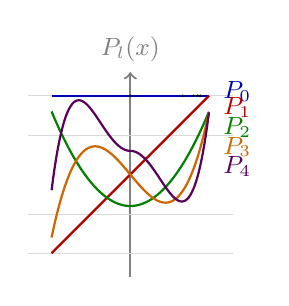
\begin{tikzpicture}[
  pde11P0/.style = {thick, blue!70!black},
  pde11P1/.style = {thick, red!70!black},
  pde11P2/.style = {thick, green!50!black},
  pde11P3/.style = {thick, orange!80!black},
  pde11P4/.style = {thick, violet!70!black},
  pde11axis/.style = {->, thick, gray},
  pde11grid/.style = {gray!30, very thin},
  pde11lbl/.style = {font=\small}
]
  % 鍧愭爣杞?  \draw[pde11axis] (-1.3,0) -- (1.3,0) node[right, pde11lbl] {$x$};
  \draw[pde11axis] (0,-1.3) -- (0,1.3) node[above, pde11lbl] {$P_l(x)$};
  % 缃戞牸
  \foreach \y in {-1,-0.5,0.5,1} {
    \draw[pde11grid] (-1.3,\y) -- (1.3,\y);
  }
  % P_0(x) = 1
  \draw[pde11P0] (-1,1) -- (1,1);
  \node[pde11P0, right, pde11lbl] at (1.05, 1.05) {$P_0$};
  % P_1(x) = x
  \draw[pde11P1] (-1,-1) -- (1,1);
  \node[pde11P1, right, pde11lbl] at (1.05, 0.85) {$P_1$};
  % P_2(x) = (3x^2-1)/2
  \draw[pde11P2, domain=-1:1, samples=100]
    plot (\x, {0.8*(1.5*\x*\x - 0.5)});
  \node[pde11P2, right, pde11lbl] at (1.05, 0.6) {$P_2$};
  % P_3(x) = (5x^3-3x)/2
  \draw[pde11P3, domain=-1:1, samples=100]
    plot (\x, {0.8*(2.5*\x^3 - 1.5*\x)});
  \node[pde11P3, right, pde11lbl] at (1.05, 0.35) {$P_3$};
  % P_4(x) = (35x^4-30x^2+3)/8
  \draw[pde11P4, domain=-1:1, samples=100]
    plot (\x, {0.8*(4.375*\x^4 - 3.75*\x^2 + 0.375)});
  \node[pde11P4, right, pde11lbl] at (1.05, 0.1) {$P_4$};
  % 绔偣
  \foreach \l in {0,1,2,3,4} {
    \fill ({2*\l/(2*\l+1)},1) circle (0.5pt);
  }
\end{tikzpicture}
\caption{鍓嶄簲涓嫆璁╁痉澶氶」寮?$P_0(x)$ 鍒?$P_4(x)$ 鐨勫浘鍍弣
\end{figure}

%% ============================================================
\section{鍕掕寰峰椤瑰紡鐨勬€ц川}

\begin{myTheorem}{鍕掕寰峰椤瑰紡鐨勯浂鐐箎
$P_l(x)$ 鎭板ソ鏈?$l$ 涓簰涓嶇浉鍚岀殑瀹為浂鐐癸紝涓斿叏閮ㄤ綅浜庡尯闂?$(-1,1)$ 鍐呫€傝繖浜涢浂鐐瑰叧浜庡師鐐瑰绉板垎甯冦€?\end{myTheorem}

\begin{myTheorem}{鍔犳硶鍏紡}
璁?$\mathbf{r}_1$ 鍜?$\mathbf{r}_2$ 涓轰袱涓悜閲忥紝$\gamma$ 涓哄畠浠箣闂寸殑澶硅锛屽垯
\begin{equation}
  P_l(\cos\gamma) = P_l(\cos\theta_1)\,P_l(\cos\theta_2)
  + 2\sum_{m=1}^{l}\frac{(l-m)!}{(l+m)!}\,P_l^m(\cos\theta_1)\,P_l^m(\cos\theta_2)\,
  \cos\big[m(\varphi_1-\varphi_2)\big],
  \label{eq:legendre-addition}
\end{equation}
鍏朵腑 $\theta_i, \varphi_i$ 鏄?$\mathbf{r}_i$ 鐨勭悆鍧愭爣瑙掋€?\end{myTheorem}

\begin{myremark}
鍔犳硶鍏紡鍦?multipole 灞曞紑涓潪甯告湁鐢ㄣ€傚畠鍏佽鎴戜滑灏嗕竴涓偣鐨勫娍鑳芥寜鍙︿竴涓偣鐨勮搴﹁繘琛屽睍寮€锛岃繖鏄數鍔ㄥ姏瀛︿腑 multipole 杈愬皠鐞嗚鐨勬暟瀛﹀熀纭€銆?\end{myremark}

\begin{mydefinition}{杩炲甫鍕掕寰峰椤瑰紡}
褰?$m \neq 0$ 鏃讹紝鍕掕寰锋柟绋嬫帹骞夸负\textbf{杩炲甫鍕掕寰锋柟绋媫锛圓ssociated Legendre Equation锛夛細
\[
  (1-x^2)y'' - 2xy' + \left[l(l+1) - \frac{m^2}{1-x^2}\right]y = 0.
\]
鍏舵湁鐣岃В涓篭textbf{杩炲甫鍕掕寰峰椤瑰紡}锛圓ssociated Legendre Polynomial锛夛細
\begin{equation}
  P_l^m(x) = (-1)^m(1-x^2)^{m/2}\frac{d^m}{dx^m}P_l(x), \quad m \geq 0.
  \label{eq:assoc-legendre}
\end{equation}
瀵逛簬 $m < 0$锛屽畾涔?$P_l^{-m}(x) = (-1)^m \frac{(l-m)!}{(l+m)!}P_l^m(x)$銆?\end{mydefinition}

\begin{figure}[htbp]
\centering
\begin{tikzpicture}[
  pde11leg3d/.style = {thick, draw=blue!70!black, fill=blue!10, opacity=0.6},
  pde11axis/.style = {->, thick, gray},
  pde11lbl/.style = {font=\small}
]
  % 鍧愭爣杞?  \draw[pde11axis] (-3,0,0) -- (3,0,0) node[right, pde11lbl] {$x$};
  \draw[pde11axis] (0,0,0) -- (0,3,0) node[above, pde11lbl] {$y$};
  \draw[pde11axis] (0,0,0) -- (0,0,3) node[above left, pde11lbl] {$z$};
  % P_1(cos theta) = cos theta -> z 鏂瑰悜鍋舵瀬瀛?  % 缁樺埗鐞冮潰涓婄殑 P_1(cos theta) = cos theta 棰滆壊鏄犲皠
  \foreach \ang in {0,15,...,165} {
    \draw[pde11leg3d]
      ({2*sin(\ang)*cos(0)},{2*sin(\ang)*sin(0)},{2*cos(\ang)})
      -- ({2*sin(\ang)*cos(90)},{2*sin(\ang)*sin(90)},{2*cos(\ang)})
      -- ({2*sin(\ang)*cos(180)},{2*sin(\ang)*sin(180)},{2*cos(\ang)})
      -- ({2*sin(\ang)*cos(270)},{2*sin(\ang)*sin(270)},{2*cos(\ang)})
      -- cycle;
  }
  % 鏍囨敞
  \node[pde11lbl] at (0, 0, -0.5) {$P_1(\cos\theta)=\cos\theta$};
  % 鍋舵瀬瀛愮澶?  \draw[->, very thick, red!70!black] (0,0,-0.5) -- (0,0,2.5)
    node[midway, right, red!70!black, font=\small] {鍋舵瀬鐭﹠;
\end{tikzpicture}
\caption{$P_1(\cos\theta)=\cos\theta$ 鍦ㄧ悆闈笂鐨勫垎甯冿細瀵瑰簲鐢靛伓鏋佸瓙}
\end{figure}

%% ============================================================
\section{骞夸箟鍕掕寰峰椤瑰紡}

\begin{mydefinition}{骞夸箟鍕掕寰峰椤瑰紡}
鍦ㄥ鐞嗙悆鍧愭爣绯讳笅鐨?Legendre 鏂圭▼锛?m \neq 0$锛夋椂锛岃繛甯﹀嫆璁╁痉澶氶」寮?$P_l^m(x)$ 涓庣悆璋愬嚱鏁板瘑鍒囩浉鍏炽€傚箍涔夊嫆璁╁痉鍑芥暟鍏佽 $l$ 鍜?$m$ 鍙栭潪鏁存暟鍊硷紝姝ゆ椂瑙ｄ笉鍐嶆槸澶氶」寮忚€屾槸鏃犵┓绾ф暟銆?
瀵逛簬 $|x| > 1$锛屽彲浠ュ畾涔塡textbf{绗簩绫诲嫆璁╁痉鍑芥暟} $Q_l(x)$锛屽畠鍦?$x=\pm 1$ 澶勫彂鏁ｏ細
\[
  Q_l(x) = \frac{1}{2}P_l(x)\ln\frac{1+x}{1-x} - W_{l-1}(x),
\]
鍏朵腑 $W_{l-1}(x)$ 鏄?$l-1$ 娆″椤瑰紡銆?\end{mydefinition}

鍦ㄤ竴鑸儏鍐典笅锛屽嫆璁╁痉鏂圭▼鐨勯€氳В涓?\[
  y(x) = A\,P_l(x) + B\,Q_l(x),
\]
浣嗙敱浜?$Q_l(x)$ 鍦?$x=\pm 1$ 澶勫寮傦紝瀵逛簬鐗╃悊闂涓渶瑕佸湪鏋佽酱澶勶紙$\theta=0$ 鎴?$\theta=\pi$锛屽嵆 $x=\pm 1$锛夋湁鐣岀殑瑙ｏ紝$B$ 蹇呴』涓洪浂銆?
\begin{myremark}
$Q_l(x)$ 鍦ㄧ悆澹冲尯鍩燂紙$r_1 < r < r_2$锛夌殑闂涓湁鐢ㄣ€備緥濡傦紝鍦ㄤ袱涓悓蹇冪悆澹充箣闂存眰瑙?Laplace 鏂圭▼鏃讹紝瑙ｄ腑浼氬悓鏃跺寘鍚?$P_l(x)$ 鍜?$Q_l(x)$銆?\end{myremark}

%% ============================================================
\section{鐞冭皭鍑芥暟}

\begin{mydefinition}{鐞冭皭鍑芥暟}
\textbf{鐞冭皭鍑芥暟}锛圫pherical Harmonics锛夊畾涔変负
\begin{equation}
  Y_l^m(\theta,\varphi) = N_l^m\,P_l^{|m|}(\cos\theta)\,e^{im\varphi},
  \label{eq:spherical-harmonic}
\end{equation}
鍏朵腑 $l=0,1,2,\dots$锛?m=-l,-l+1,\dots,l$锛屽綊涓€鍖栫郴鏁?\[
  N_l^m = \sqrt{\frac{2l+1}{4\pi}\frac{(l-|m|)!}{(l+|m|)!}}.
\]
\end{mydefinition}

\begin{myTheorem}{鐞冭皭鍑芥暟鐨勬€ц川}
\begin{enumerate}
  \item \textbf{姝ｄ氦鎬锛?  \[
    \int_0^{2\pi}\int_0^{\pi} Y_l^{m*}(\theta,\varphi)\,Y_{l'}^{m'}(\theta,\varphi)
    \sin\theta\,d\theta\,d\varphi = \delta_{ll'}\delta_{mm'}.
  \]
  \item \textbf{瀹屽鎬锛?\{Y_l^m\}$ 鏋勬垚 $L^2(S^2)$ 涓殑瀹屽姝ｄ氦绯伙紝浠绘剰骞虫柟鍙Н鐨勭悆闈㈠嚱鏁伴兘鍙互灞曞紑涓虹悆璋愬嚱鏁扮殑绾ф暟銆?  \item \textbf{Laplace 绠楀瓙鐨勭壒寰佸嚱鏁皚锛?  \[
    \Delta_{S^2} Y_l^m = -l(l+1)\,Y_l^m,
  \]
  鍏朵腑 $\Delta_{S^2}$ 鏄悆闈笂鐨?Laplace--Beltrami 绠楀瓙銆?  \item \textbf{澶嶅叡杞叧绯粆锛?Y_l^{m*} = (-1)^m Y_l^{-m}$銆?\end{enumerate}
\end{myTheorem}

鐞冭皭鍑芥暟鍦ㄩ噺瀛愬姏瀛︿腑鍏锋湁鏍稿績鍦颁綅銆傚湪姘㈠師瀛愮殑钖涘畾璋旀柟绋嬩腑锛岃鍚戦儴鍒嗙殑瑙ｆ鏄悆璋愬嚱鏁?$Y_l^m(\theta,\varphi)$锛屽叾涓?$l$ 鏄閲忓瓙鏁帮紝$m$ 鏄閲忓瓙鏁般€?
\begin{figure}[htbp]
\centering
\begin{tikzpicture}[
  pde11orbital/.style = {thick, draw=blue!70!black, fill=blue!15, opacity=0.7},
  pde11orbital2/.style = {thick, draw=red!70!black, fill=red!15, opacity=0.7},
  pde11axis/.style = {->, thick, gray},
  pde11lbl/.style = {font=\small}
]
  % s 杞ㄩ亾 (l=0, m=0)
  \begin{scope}[shift={(0,0)}]
    \draw[pde11orbital] (0,0) circle (1cm);
    \node[pde11lbl] at (0, -1.5) {$Y_0^0$ (s 杞ㄩ亾)};
  \end{scope}
  % p_z 杞ㄩ亾 (l=1, m=0)
  \begin{scope}[shift={(4,0)}]
    \draw[pde11orbital] (0,0) ellipse (0.6cm and 1.2cm);
    \draw[pde11orbital2] (0,0) ellipse (0.6cm and 0.8cm);
    \draw[pde11axis] (-1.5,0) -- (1.5,0);
    \draw[pde11axis] (0,-1.8) -- (0,1.8);
    \node[pde11lbl] at (0, -2.2) {$Y_1^0$ (p$_z$ 杞ㄩ亾)};
  \end{scope}
  % d_{z^2} 杞ㄩ亾 (l=2, m=0)
  \begin{scope}[shift={(8,0)}]
    \draw[pde11orbital] (0,0) ellipse (0.4cm and 1.4cm);
    \draw[pde11orbital2] (0,0) ellipse (0.8cm and 0.35cm);
    \draw[pde11axis] (-1.8,0) -- (1.8,0);
    \draw[pde11axis] (0,-1.8) -- (0,1.8);
    \node[pde11lbl] at (0, -2.2) {$Y_2^0$ (d$_{z^2}$ 杞ㄩ亾)};
  \end{scope}
\end{tikzpicture}
\caption{鐞冭皭鍑芥暟 $Y_l^0$ 鐨勮鍚戝垎甯冿紙瀵瑰簲鍘熷瓙杞ㄩ亾 s銆乸$_z$銆乨$_{z^2}$锛墋
\end{figure}

\begin{lstlisting}[language=Python, caption={鐞冭皭鍑芥暟鍙鍖杴]
import numpy as np
import matplotlib.pyplot as plt
from scipy.special import lpmv, factorial

def spherical_harmonic(l, m, theta, phi):
    """璁＄畻鐞冭皭鍑芥暟 Y_l^m(theta, phi)"""
    m_abs = abs(m)
    norm = np.sqrt((2*l+1) / (4*np.pi) * factorial(l-m_abs) / factorial(l+m_abs))
    leg = lpmv(m_abs, l, np.cos(theta))
    if m >= 0:
        return norm * leg * np.cos(m * phi)
    else:
        return norm * leg * np.sin(m_abs * phi)

# 鍒涘缓鐞冮潰缃戞牸
theta = np.linspace(0, np.pi, 100)
phi = np.linspace(0, 2*np.pi, 100)
THETA, PHI = np.meshgrid(theta, phi)

# 缁樺埗 Y_1^0 鍜?Y_2^1 鐨勮鍚戝垎甯?fig = plt.figure(figsize=(12, 5))

for idx, (l, m, title) in enumerate([(1, 0, '$Y_1^0$'), (2, 1, '$Y_2^1$')]):
    ax = fig.add_subplot(1, 2, idx+1, projection='polar')
    Y = spherical_harmonic(l, m, THETA, PHI)
    c = ax.contourf(PHI, THETA, Y, levels=50, cmap='RdBu_r')
    plt.colorbar(c, ax=ax, shrink=0.8)
    ax.set_title(f'{title} 鐨勮鍚戝垎甯?, fontsize=13)
    ax.set_theta_zero_location('N')
    ax.set_theta_direction(-1)

plt.tight_layout()
plt.show()
\end{lstlisting}

\begin{myremark}
鐞冭皭鍑芥暟鐨勭墿鐞嗘剰涔夛細$|Y_l^m(\theta,\varphi)|^2$ 琛ㄧず鍦ㄦ柟鍚?$(\theta,\varphi)$ 鎵惧埌绮掑瓙鐨勬鐜囧瘑搴︼紙閲忓瓙鍔涘涓級銆?l$ 鍐冲畾浜嗚鍚戝垎甯冪殑澶嶆潅绋嬪害锛堣妭鐐规暟锛夛紝$m$ 鍐冲畾浜嗗鏂逛綅瑙?$\varphi$ 鐨勪緷璧栧叧绯汇€?l=0$ 瀵瑰簲鐞冨绉板垎甯冿紝$l$ 瓒婂ぇ鍒嗗竷瓒婂鏉傘€?\end{myremark}

鐞冭皭鍑芥暟鍦?multipole 灞曞紑涓篃鏈夋牳蹇冨簲鐢ㄣ€傛爣閲忓娍 $1/|\mathbf{r}-\mathbf{r}'|$ 鍙互灞曞紑涓?\[
  \frac{1}{|\mathbf{r}-\mathbf{r}'|}
  = 4\pi\sum_{l=0}^{\infty}\sum_{m=-l}^{l}
  \frac{1}{2l+1}\frac{r_<^l}{r_>^{l+1}}\,Y_l^{m*}(\theta',\varphi')\,Y_l^m(\theta,\varphi),
\]
鍏朵腑 $r_<=\min(r,r')$锛?r_>=\max(r,r')$銆?
%% ============================================================
\section*{鏈珷灏忕粨}

鏈珷绯荤粺浠嬬粛浜嗗嫆璁╁痉澶氶」寮忓強鍏剁浉鍏冲嚱鏁帮細
\begin{itemize}
  \item 鍕掕寰锋柟绋嬫槸鐞冨潗鏍囩郴涓嬪垎绂诲彉閲忎骇鐢熺殑鍏稿瀷甯稿井鍒嗘柟绋嬶紱
  \item 鍕掕寰峰椤瑰紡 $P_l(x)$ 鐢?Rodrigues 鍏紡瀹氫箟锛屽湪 $[-1,1]$ 涓婃瀯鎴愬畬澶囨浜ょ郴锛?  \item 杩炲甫鍕掕寰峰椤瑰紡 $P_l^m(x)$ 鏄?$m \neq 0$ 鏃剁殑鎺ㄥ箍锛?  \item 鐞冭皭鍑芥暟 $Y_l^m(\theta,\varphi)$ 鏄悆闈笂 Laplace 绠楀瓙鐨勭壒寰佸嚱鏁帮紝鍦ㄩ噺瀛愬姏瀛﹀拰鐢电瀛︿腑鏈夋牳蹇冨湴浣嶏紱
  \item Multipole 灞曞紑鍒╃敤鐞冭皭鍑芥暟灏嗗娍鍑芥暟鍒嗚В涓轰笉鍚岃鍔ㄩ噺鐨勮础鐚€?\end{itemize}

%% ============================================================
\section*{缁冧範棰榼

\begin{enumerate}
  \item 鍒╃敤 Rodrigues 鍏紡楠岃瘉 $P_2(x) = \frac{1}{2}(3x^2-1)$銆?
  \item 璇佹槑鍕掕寰峰椤瑰紡鐨勯€掓帹鍏崇郴锛?  \[
    (l+1)P_{l+1}(x) = (2l+1)\,x\,P_l(x) - l\,P_{l-1}(x).
  \]

  \item 鍒╃敤姝ｄ氦鎬ц绠?$f(x) = x^3$ 鍦?$L^2([-1,1])$ 涓叧浜?$\{P_l\}$ 鐨勫睍寮€绯绘暟 $c_0, c_1, c_2, c_3$銆?
  \item 璇佹槑鐞冭皭鍑芥暟鐨勬浜ゆ€э紙鍙獙璇?$l=0$ 鍜?$l=1$ 鐨勬儏褰級銆?
  \item 鍒╃敤 Python 缁樺埗 $Y_2^1(\theta,\varphi)$ 鐨勪笁缁磋鍚戝垎甯冨浘銆?\end{enumerate}

\chapter{鍏朵粬鐗规畩鍑芥暟}

\section*{寮曡█}

闄や簡璐濆灏斿嚱鏁板拰鍕掕寰峰椤瑰紡涔嬪锛屾暟瀛︾墿鐞嗕腑杩樻湁璁稿鍏朵粬閲嶈鐨勭壒娈婂嚱鏁般€傝繖浜涚壒娈婂嚱鏁板垎鍒湪涓嶅悓鐨勭墿鐞嗛棶棰樺拰鍧愭爣绯讳腑鍑虹幇锛屽悇鑷叿鏈夌嫭鐗圭殑鎬ц川鍜屽簲鐢ㄣ€傛湰绔犲皢浠嬬粛鍑犵被鏈€甯哥敤鐨勭壒娈婂嚱鏁帮細鍘勭背澶氶」寮忥紙Hermite Polynomials锛夈€佹媺鐩栧皵澶氶」寮忥紙Laguerre Polynomials锛夈€佽秴鍑犱綍鍑芥暟锛圚ypergeometric Functions锛夈€丟amma 鍑芥暟鍜?Beta 鍑芥暟锛屼互鍙婃き鍦嗗嚱鏁扮殑绠€浠嬨€?
杩欎簺鐗规畩鍑芥暟鍙互缁熶竴鍦ㄦ洿涓€鑸殑妗嗘灦涓嬬悊瑙ｃ€備簨瀹炰笂锛岃澶氱壒娈婂嚱鏁伴兘鏄煇浜涚壒瀹氱殑浜岄樁绾挎€у父寰垎鏂圭▼鐨勮В锛岃€岃繖浜涙柟绋嬫湰韬張鍙互閫氳繃閫傚綋鐨勫彉鎹㈢浉浜掕仈绯汇€傜悊瑙ｈ繖浜涜仈绯绘湁鍔╀簬寤虹珛瀹屾暣鐨勭壒娈婂嚱鏁扮悊璁轰綋绯汇€?
\begin{myremark}
鐗规畩鍑芥暟鐞嗚鏄?19 涓栫邯鏁板鐨勯噸瑕佹垚灏变箣涓€銆侴auss銆丣acobi銆乄eierstrass銆丷iemann 绛変汉閮藉鐗规畩鍑芥暟鐞嗚鍋氬嚭浜嗗鍩烘€ц础鐚€傜幇浠ｆ暟瀛︾墿鐞嗕腑锛岀壒娈婂嚱鏁扮悊璁轰笌缇よ銆佽〃绀鸿鏈夌潃娣卞埢鐨勮仈绯汇€?\end{myremark}

%% ============================================================
\section{鍘勭背澶氶」寮弣

\begin{mydefinition}{鍘勭背鏂圭▼涓庡巹绫冲椤瑰紡}
\textbf{鍘勭背鏂圭▼}锛圚ermite Equation锛夋槸鎸囧涓嬩簩闃剁嚎鎬у父寰垎鏂圭▼锛?\begin{equation}
  y'' - 2x\,y' + 2n\,y = 0, \quad n = 0,1,2,\dots
  \label{eq:hermite}
\end{equation}
鍏跺湪 $(-\infty,+\infty)$ 涓婃湁鐣岀殑瑙ｆ槸 $n$ 娆″椤瑰紡锛岀О涓篭textbf{鍘勭背澶氶」寮弣锛圚ermite Polynomial锛夛紝璁颁负 $H_n(x)$銆傚畠鍙互鐢?Rodrigues 鍏紡瀹氫箟锛?\begin{equation}
  H_n(x) = (-1)^n\,e^{x^2}\frac{d^n}{dx^n}e^{-x^2}.
  \label{eq:hermite-rod}
\end{equation}
\end{mydefinition}

鍘勭背澶氶」寮忕殑鍓嶅嚑椤逛负
\begin{align}
  H_0(x) &= 1, \notag \\
  H_1(x) &= 2x, \notag \\
  H_2(x) &= 4x^2 - 2, \notag \\
  H_3(x) &= 8x^3 - 12x, \notag \\
  H_4(x) &= 16x^4 - 48x^2 + 12.
  \label{eq:hermite-first-few}
\end{align}

\begin{myTheorem}{鍘勭背澶氶」寮忕殑鎬ц川}
\begin{enumerate}
  \item \textbf{閫掓帹鍏崇郴}锛?H_{n+1}(x) = 2x\,H_n(x) - 2n\,H_{n-1}(x)$銆?  \item \textbf{瀵兼暟鍏崇郴}锛?H_n'(x) = 2n\,H_{n-1}(x)$銆?  \item \textbf{姝ｄ氦鎬锛氬叧浜庢潈閲嶅嚱鏁?$e^{-x^2}$ 姝ｄ氦锛?  \[
    \int_{-\infty}^{+\infty} H_m(x)\,H_n(x)\,e^{-x^2}\,dx
    = \sqrt{\pi}\,2^n\,n!\,\delta_{mn}.
  \]
  \item \textbf{鐢熸垚鍑芥暟}锛?  \[
    e^{2xt-t^2} = \sum_{n=0}^{\infty}\frac{H_n(x)}{n!}\,t^n.
  \]
\end{enumerate}
\end{myTheorem}

\begin{figure}[htbp]
\centering
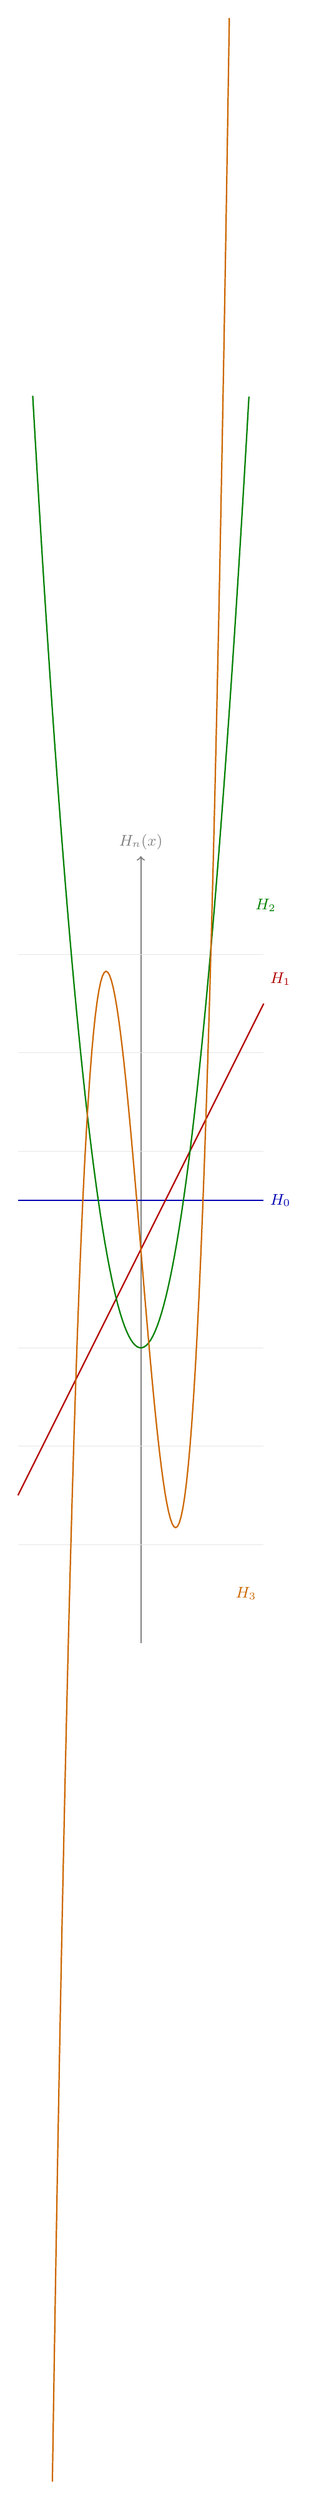
\begin{tikzpicture}[
  pde12H0/.style = {thick, blue!70!black},
  pde12H1/.style = {thick, red!70!black},
  pde12H2/.style = {thick, green!50!black},
  pde12H3/.style = {thick, orange!80!black},
  pde12H4/.style = {thick, violet!70!black},
  pde12axis/.style = {->, thick, gray},
  pde12grid/.style = {gray!20, very thin},
  pde12lbl/.style = {font=\small}
]
  % 鍧愭爣杞?  \draw[pde12axis] (-2.5,0) -- (2.5,0) node[right, pde12lbl] {$x$};
  \draw[pde12axis] (0,-8) -- (0,8) node[above, pde12lbl] {$H_n(x)$};
  % 缃戞牸
  \foreach \y in {-6,-4,-2,2,4,6} {
    \draw[pde12grid] (-2.5,\y) -- (2.5,\y);
  }
  % H_0(x) = 1
  \draw[pde12H0] (-2.5,1) -- (2.5,1);
  % H_1(x) = 2x
  \draw[pde12H1] (-2.5,-5) -- (2.5,5);
  % H_2(x) = 4x^2 - 2
  \draw[pde12H2, domain=-2.2:2.2, samples=100]
    plot (\x, {4*\x*\x - 2});
  % H_3(x) = 8x^3 - 12x
  \draw[pde12H3, domain=-1.8:1.8, samples=100]
    plot (\x, {8*\x^3 - 12*\x});
  % 鏍囨敞
  \node[pde12H0, right, pde12lbl] at (2.5, 1) {$H_0$};
  \node[pde12H1, right, pde12lbl] at (2.5, 5.5) {$H_1$};
  \node[pde12H2, right, pde12lbl] at (2.2, 7) {$H_2$};
  \node[pde12H3, right, pde12lbl] at (1.8, -7) {$H_3$};
\end{tikzpicture}
\caption{鍓嶅洓涓巹绫冲椤瑰紡鐨勫浘鍍弣
\end{figure}

鍘勭背澶氶」寮忓湪閲忓瓙鍔涘涓湁鏍稿績鍦颁綅銆備竴缁磋皭鎸瓙鐨勮枦瀹氳皵鏂圭▼鐨勬湰寰佸嚱鏁颁负
\[
  \psi_n(x) = \left(\frac{m\omega}{\pi\hbar}\right)^{1/4}
  \frac{1}{\sqrt{2^n\,n!}}\,H_n\!\left(\sqrt{\frac{m\omega}{\hbar}}\,x\right)
  \,e^{-m\omega x^2/(2\hbar)},
\]
瀵瑰簲鐨勮兘閲忔湰寰佸€间负 $E_n = \hbar\omega(n+1/2)$銆?
\begin{myremark}
鍘勭背澶氶」寮忚繕鍑虹幇鍦ㄦ鐜囪锛圚ermite 澶氶」寮忔槸姝ｆ€佸垎甯冪殑姝ｄ氦澶氶」寮忥級銆佸亸寰垎鏂圭▼锛堢儹鏂圭▼鐨勬煇浜涚壒娈婅В锛夈€佷互鍙婃暟鍊煎垎鏋愶紙 Gauss--Hermite 姹傜Н鍏紡锛変腑銆?\end{myremark}

%% ============================================================
\section{鎷夌洊灏斿椤瑰紡}

\begin{mydefinition}{鎷夌洊灏旀柟绋嬩笌鎷夌洊灏斿椤瑰紡}
\textbf{鎷夌洊灏旀柟绋媫锛圠aguerre Equation锛夋槸鎸?\begin{equation}
  x\,y'' + (1-x)\,y' + n\,y = 0, \quad n = 0,1,2,\dots
  \label{eq:laguerre}
\end{equation}
鍏舵湁鐣岃В涓篭textbf{鎷夌洊灏斿椤瑰紡}锛圠aguerre Polynomial锛?L_n(x)$锛?\begin{equation}
  L_n(x) = \sum_{k=0}^{n}\frac{(-1)^k}{k!}\binom{n}{k}x^k
  = \sum_{k=0}^{n}\frac{(-1)^k\,n!}{(k!)^2\,(n-k)!}\,x^k.
  \label{eq:laguerre-def}
\end{equation}
\end{mydefinition}

\begin{mydefinition}{杩炲甫鎷夌洊灏斿椤瑰紡}
\textbf{杩炲甫鎷夌洊灏斿椤瑰紡}锛圓ssociated Laguerre Polynomial锛夊畾涔変负
\begin{equation}
  L_n^k(x) = (-1)^k\frac{d^k}{dx^k}L_{n+k}(x)
  = \sum_{j=0}^{n}\frac{(-1)^j\,(n+k)!}{(j!)^2\,(n-j)!\,(k+j)!}\,x^{k+j}.
  \label{eq:assoc-laguerre}
\end{equation}
鐗瑰埆鍦帮紝$L_n^0(x) = L_n(x)$銆?\end{mydefinition}

\begin{myTheorem}{鎷夌洊灏斿椤瑰紡鐨勬€ц川}
\begin{enumerate}
  \item \textbf{姝ｄ氦鎬锛氬叧浜庢潈閲?$e^{-x}$ 姝ｄ氦锛?  \[
    \int_0^{+\infty} L_m(x)\,L_n(x)\,e^{-x}\,dx = \delta_{mn}.
  \]
  \item \textbf{杩炲甫鎷夌洊灏斿椤瑰紡鐨勬浜ゆ€锛?  \[
    \int_0^{+\infty} L_m^k(x)\,L_n^k(x)\,x^k\,e^{-x}\,dx
    = \frac{(n+k)!}{n!}\,\delta_{mn}.
  \]
  \item \textbf{閫掓帹鍏崇郴}锛?(n+1)L_{n+1}(x) = (2n+1-x)L_n(x) - n\,L_{n-1}(x)$銆?\end{enumerate}
\end{myTheorem}

鎷夌洊灏斿椤瑰紡鍦ㄦ阿鍘熷瓙鐨勯噺瀛愬姏瀛﹂棶棰樹腑鎵紨鏍稿績瑙掕壊銆傛阿鍘熷瓙娉㈠嚱鏁扮殑寰勫悜閮ㄥ垎涓?\[
  R_{nl}(r) = N_{nl}\,e^{-r/(na_0)}\left(\frac{2r}{na_0}\right)^l
  L_{n-l-1}^{2l+1}\!\left(\frac{2r}{na_0}\right),
\]
鍏朵腑 $n$ 鏄富閲忓瓙鏁帮紝$l$ 鏄閲忓瓙鏁帮紝$a_0$ 鏄?Bohr 鍗婂緞锛?N_{nl}$ 鏄綊涓€鍖栧父鏁般€?
\begin{figure}[htbp]
\centering
\begin{tikzpicture}[
  pde12L0/.style = {thick, blue!70!black},
  pde12L1/.style = {thick, red!70!black},
  pde12L2/.style = {thick, green!50!black},
  pde12axis/.style = {->, thick, gray},
  pde12lbl/.style = {font=\small},
  pde12shade/.style = {fill=blue!5, opacity=0.3}
]
  % 鍧愭爣杞?  \draw[pde12axis] (-0.3,0) -- (12,0) node[right, pde12lbl] {$x$};
  \draw[pde12axis] (0,-1.5) -- (0,2.5) node[above, pde12lbl] {$L_n(x)$};
  % L_0(x) = 1
  \draw[pde12L0] (0,1) -- (11,1);
  \node[pde12L0, right, pde12lbl] at (11.2, 1.0) {$L_0$};
  % L_1(x) = 1 - x
  \draw[pde12L1] (0,1) -- (11,-1);
  \node[pde12L1, right, pde12lbl] at (11.2, -0.8) {$L_1$};
  % L_2(x) = 1 - 2x + x^2/2
  \draw[pde12L2, domain=0:10.5, samples=200]
    plot (\x, {1 - 2*\x + 0.5*\x*\x});
  \node[pde12L2, right, pde12lbl] at (10.7, 2.2) {$L_2$};
  % 鏉冮噸鍑芥暟 e^{-x} 鐨勭ず鎰?  \draw[dashed, gray, domain=0:8, samples=100]
    plot (\x, {2*exp(-\x)});
  \node[pde12lbl, gray] at (5, 2.0) {$e^{-x}$锛堟潈閲嶏級};
  % 鏍囨敞
  \node[pde12lbl] at (5.5, -1.2) {鎷夌洊灏斿椤瑰紡锛?[0,+\infty)$ 涓婂叧浜?$e^{-x}$ 姝ｄ氦};
\end{tikzpicture}
\caption{鎷夌洊灏斿椤瑰紡鍙婂叾鏉冮噸鍑芥暟}
\end{figure}

\begin{lstlisting}[language=Python, caption={鍘勭背澶氶」寮忓拰鎷夌洊灏斿椤瑰紡鐨勫彲瑙嗗寲}]
import numpy as np
import matplotlib.pyplot as plt
from scipy.special import hermite, eval_hermite, eval_laguerre

# 鍘勭背澶氶」寮?x_h = np.linspace(-3, 3, 200)
fig, (ax1, ax2) = plt.subplots(1, 2, figsize=(14, 5))

for n in range(5):
    y = eval_hermite(n, x_h) * np.exp(-x_h**2)
    ax1.plot(x_h, y, linewidth=2, label=f'$H_{n}(x)e^{{-x^2}}$')
ax1.set_title('鍘勭背澶氶」寮忓姞鏉?$H_n(x)e^{-x^2}$', fontsize=13)
ax1.set_xlabel('$x$')
ax1.legend(fontsize=10)
ax1.grid(True, alpha=0.3)
ax1.set_xlim(-3, 3)

# 鎷夌洊灏斿椤瑰紡
x_l = np.linspace(0, 12, 300)
for n in range(5):
    y = eval_laguerre(n, x_l) * np.exp(-x_l)
    ax2.plot(x_l, y, linewidth=2, label=f'$L_{n}(x)e^{{-x}}$')
ax2.set_title('鎷夌洊灏斿椤瑰紡鍔犳潈 $L_n(x)e^{-x}$', fontsize=13)
ax2.set_xlabel('$x$')
ax2.legend(fontsize=10)
ax2.grid(True, alpha=0.3)
ax2.set_xlim(0, 12)
ax2.set_ylim(-1.5, 2)

plt.tight_layout()
plt.show()
\end{lstlisting}

%% ============================================================
\section{瓒呭嚑浣曞嚱鏁皚

\begin{mydefinition}{瓒呭嚑浣曟柟绋嬩笌瓒呭嚑浣曞嚱鏁皚
\textbf{Gauss 瓒呭嚑浣曟柟绋媫锛圙auss Hypergeometric Equation锛夋槸鎸?\begin{equation}
  x(1-x)\,y'' + [c-(a+b+1)x]\,y' - ab\,y = 0,
  \label{eq:hypergeometric}
\end{equation}
鍏朵腑 $a,b,c$ 涓哄弬鏁帮紙$c$ 涓嶆槸闈炴鏁存暟锛夈€傛柟绋嬪湪 $x=0$ 澶勭殑姝ｅ垯瑙ｅ畾涔変负\textbf{瓒呭嚑浣曞嚱鏁皚锛圚ypergeometric Function锛夛細
\begin{equation}
  F(a,b;c;x) = {}_2F_1(a,b;c;x)
  = \sum_{n=0}^{\infty}\frac{(a)_n\,(b)_n}{(c)_n\,n!}\,x^n,
  \label{eq:hypergeometric-def}
\end{equation}
鍏朵腑 $(a)_n = a(a+1)\cdots(a+n-1)$ 涓?Pochhammer 绗﹀彿锛堜笂鍗囬樁涔樺箓锛夛紝$(a)_0 = 1$銆?\end{mydefinition}

瓒呭嚑浣曞嚱鏁版槸涓€涓潪甯镐竴鑸殑鐗规畩鍑芥暟锛岃澶氬父瑙佺壒娈婂嚱鏁伴兘鏄畠鐨勭壒渚嬶細

\begin{myTheorem}{鐗规畩鍑芥暟鐨勮秴鍑犱綍琛ㄧず}
\begin{enumerate}
  \item \textbf{鍕掕寰峰椤瑰紡}锛?P_l(x) = F(-l,l+1;1;\frac{1-x}{2})$銆?  \item \textbf{Chebyshev 澶氶」寮弣锛?T_n(x) = F(-n,n;\frac{1}{2};\frac{1-x}{2})$銆?  \item \textbf{鍑犱綍绾ф暟}锛?F(1,b;b;x) = \frac{1}{1-x}$銆?  \item \textbf{浜岄」寮忓睍寮€}锛?F(-n,b;b;-x) = (1+x)^n$銆?  \item \textbf{鍙嶆寮﹀嚱鏁皚锛?\arcsin x = x\,F\!\left(\frac{1}{2},\frac{1}{2};\frac{3}{2};x^2\right)$銆?\end{enumerate}
\end{myTheorem}

瓒呭嚑浣曞嚱鏁板湪澶勭悊 Legendre 鏂圭▼銆丆hebyshev 鏂圭▼绛変簩闃剁嚎鎬?ODE 鏃堕潪甯告湁鐢ㄣ€傚畠浠繕鍑虹幇鍦ㄩ噺瀛愭暎灏勭悊璁猴紙Coulomb 鏁ｅ皠锛夈€佸箍涔夌浉瀵硅鍜岀粺璁″姏瀛︿腑銆?
\begin{figure}[htbp]
\centering
\begin{tikzpicture}[
  pde12hyper/.style = {thick},
  pde12axis/.style = {->, thick, gray},
  pde12lbl/.style = {font=\small}
]
  % 鍧愭爣杞?  \draw[pde12axis] (-0.3,0) -- (2,0) node[right, pde12lbl] {$x$};
  \draw[pde12axis] (0,-0.3) -- (0,3) node[above, pde12lbl] {$F(a,b;c;x)$};
  % F(1,1;1;x) = 1/(1-x)
  \draw[pde12hyper, blue!70!black, domain=0:0.85, samples=100]
    plot ({\x}, {1/(1-\x)});
  \node[pde12lbl, blue!70!black] at (0.5, 2.5) {$F(1,1;1;x)=\frac{1}{1-x}$};
  % F(1/2,1/2;3/2;x^2) -> arcsin/sqrt
  \draw[pde12hyper, red!70!black, domain=0:0.95, samples=100]
    plot ({\x}, {asin(\x)/sqrt(1-\x*\x+0.01)});
  \node[pde12lbl, red!70!black] at (1.3, 1.8) {$\arcsin x / \sqrt{1-x^2}$};
  % F(-1,1;1;(1-x)/2) = P_1(x) = x
  \draw[pde12hyper, green!50!black] (0,0) -- (1.5,1.5);
  \node[pde12lbl, green!50!black] at (1.5, 1.7) {$P_1(x)=x$};
  % 鏍囨敞
  \node[pde12lbl] at (1, -0.2) {$[0,1)$};
\end{tikzpicture}
\caption{瓒呭嚑浣曞嚱鏁扮殑鍑犱釜鐗逛緥}
\end{figure}

%% ============================================================
\section{Gamma 鍑芥暟鍜?Beta 鍑芥暟}

\begin{mydefinition}{Gamma 鍑芥暟}
\textbf{Gamma 鍑芥暟}锛圙amma Function锛?\Gamma(z)$ 鏄樁涔樺嚱鏁板湪澶嶆暟鍩熶笂鐨勬帹骞匡紝瀹氫箟涓?\begin{equation}
  \Gamma(z) = \int_0^{+\infty} t^{z-1}\,e^{-t}\,dt, \quad \text{Re}(z) > 0.
  \label{eq:gamma}
\end{equation}
閫氳繃瑙ｆ瀽寤舵嫇鍙互瀹氫箟鍦ㄩ櫎 $z=0,-1,-2,\dots$ 涔嬪鐨勬暣涓骞抽潰涓娿€?\end{mydefinition}

\begin{myTheorem}{Gamma 鍑芥暟鐨勫熀鏈€ц川}
\begin{enumerate}
  \item \textbf{閫掓帹鍏崇郴}锛?\Gamma(z+1) = z\,\Gamma(z)$銆?  \item \textbf{涓庨樁涔樼殑鍏崇郴}锛?\Gamma(n+1) = n!$锛?n$ 涓洪潪璐熸暣鏁帮級銆?  \item \textbf{鍙嶅皠鍏紡}锛?\Gamma(z)\,\Gamma(1-z) = \frac{\pi}{\sin(\pi z)}$銆?  \item \textbf{Legendre 鍊嶅厓鍏紡}锛?\Gamma(z)\,\Gamma(z+\frac{1}{2}) = \frac{\sqrt{\pi}}{2^{2z-1}}\,\Gamma(2z)$銆?  \item \textbf{鐗规畩鍊紏锛?\Gamma\!\left(\frac{1}{2}\right) = \sqrt{\pi}$锛?\Gamma(1) = 1$銆?\end{enumerate}
\end{myTheorem}

\begin{mydefinition}{Beta 鍑芥暟}
\textbf{Beta 鍑芥暟}锛圔eta Function锛?B(p,q)$ 瀹氫箟涓?\begin{equation}
  B(p,q) = \int_0^1 t^{p-1}(1-t)^{q-1}\,dt, \quad \text{Re}(p),\text{Re}(q) > 0.
  \label{eq:beta}
\end{equation}
Beta 鍑芥暟涓?Gamma 鍑芥暟鐨勫叧绯讳负
\[
  B(p,q) = \frac{\Gamma(p)\,\Gamma(q)}{\Gamma(p+q)}.
\]
\end{mydefinition}

Gamma 鍑芥暟鍜?Beta 鍑芥暟鍦ㄧ壒娈婂嚱鏁扮悊璁轰腑鏈夊熀纭€鍦颁綅銆傚嚑涔庢墍鏈夌壒娈婂嚱鏁扮殑褰掍竴鍖栫郴鏁般€佹浜ゆ€у叕寮忓拰绉垎琛ㄧず閮芥秹鍙?Gamma 鍑芥暟銆侭eta 鍑芥暟鍒欏湪姒傜巼缁熻锛圔eta 鍒嗗竷锛夊拰澶氶噸绉垎涓湁骞挎硾搴旂敤銆?
\begin{figure}[htbp]
\centering
\begin{tikzpicture}[
  pde12gamma/.style = {thick, blue!70!black},
  pde12gamma2/.style = {thick, red!70!black, dashed},
  pde12axis/.style = {->, thick, gray},
  pde12lbl/.style = {font=\small}
]
  % 鍧愭爣杞?  \draw[pde12axis] (-0.5,0) -- (5,0) node[right, pde12lbl] {$x$};
  \draw[pde12axis] (0,-0.5) -- (0,5) node[above, pde12lbl] {$\Gamma(x)$};
  % Gamma(x) for x > 0
  \draw[pde12gamma, domain=0.3:5, samples=200]
    plot (\x, {gamma(\x)});
  % 鏍囨敞鐗规畩鍊?  \fill[blue!70!black] (1,1) circle (2pt);
  \node[pde12lbl, below right] at (1,1) {$\Gamma(1)=0!=1$};
  \fill[blue!70!black] (2,1) circle (2pt);
  \node[pde12lbl, below right] at (2,1) {$\Gamma(2)=1!=1$};
  \fill[blue!70!black] (3,2) circle (2pt);
  \node[pde12lbl, below right] at (3,2) {$\Gamma(3)=2!=2$};
  \fill[blue!70!black] (4,6) circle (2pt);
  \node[pde12lbl, below right] at (4,4.5) {$\Gamma(4)=3!=6$};
  \fill[blue!70!black] (0.5,1.77) circle (2pt);
  \node[pde12lbl, left] at (0.5,1.77) {$\Gamma(\frac{1}{2})=\sqrt{\pi}$};
  % 娓愯繎绾?  \draw[dashed, gray] (0.3,0) -- (0.3,4.5);
  \node[pde12lbl, gray] at (0.1, 3) {$x=0$锛堟瀬鐐癸級};
\end{tikzpicture}
\caption{Gamma 鍑芥暟 $\Gamma(x)$ 鐨勫浘鍍弣
\end{figure}

%% ============================================================
\section{妞渾鍑芥暟绠€浠媫

\begin{mydefinition}{妞渾绉垎}
\textbf{妞渾绉垎}锛圗lliptic Integral锛夋槸涓€绫讳笉鑳界敤鍒濈瓑鍑芥暟琛ㄧず鐨勭Н鍒嗐€傜涓€绫诲畬鍏ㄦき鍦嗙Н鍒嗗畾涔変负
\begin{equation}
  K(k) = \int_0^{\pi/2}\frac{d\theta}{\sqrt{1-k^2\sin^2\theta}},
  \quad |k| < 1,
  \label{eq:elliptic-K}
\end{equation}
鍏朵腑 $k$ 绉颁负妯℃暟锛坢odulus锛夈€?绗簩绫诲畬鍏ㄦき鍦嗙Н鍒嗕负
\[
  E(k) = \int_0^{\pi/2}\sqrt{1-k^2\sin^2\theta}\,d\theta.
\]
\end{mydefinition}

妞渾绉垎鏉ユ簮浜庤绠楁き鍦嗗姬闀裤€佸崟鎽嗗懆鏈熺瓑瀹為檯闂銆備緥濡傦紝鍗曟憜鐨勭簿纭懆鏈熶负
\[
  T = 4\sqrt{\frac{l}{g}}\,K\!\left(\sin\frac{\theta_0}{2}\right),
\]
鍏朵腑 $l$ 鏄憜闀匡紝$\theta_0$ 鏄垵濮嬭搴︺€?
\begin{mydefinition}{妞渾鍑芥暟}
\textbf{Jacobi 妞渾鍑芥暟}鏄き鍦嗙Н鍒嗙殑鍙嶅嚱鏁般€傝
\[
  u = \int_0^{\phi}\frac{d\theta}{\sqrt{1-k^2\sin^2\theta}},
\]
鍒?$\text{sn}(u,k) = \sin\phi$锛?\text{cn}(u,k) = \cos\phi$锛?\text{dn}(u,k) = \sqrt{1-k^2\sin^2\phi}$ 鍒嗗埆绉颁负 Jacobi 妞渾姝ｅ鸡銆佷綑寮﹀拰 delta 鍑芥暟銆?
\textbf{Weierstrass 妞渾鍑芥暟} $\wp(z)$ 鏄弻鍛ㄦ湡澶嶅嚱鏁帮紝婊¤冻寰垎鏂圭▼
\[
  (\wp')^2 = 4\wp^3 - g_2\,\wp - g_3,
\]
鍏朵腑 $g_2, g_3$ 鏄笌鍛ㄦ湡鐩稿叧鐨勫父鏁般€?\end{mydefinition}

\begin{figure}[htbp]
\centering
\begin{tikzpicture}[
  pde12sn/.style = {thick, blue!70!black},
  pde12cn/.style = {thick, red!70!black},
  pde12dn/.style = {thick, green!50!black},
  pde12sin/.style = {thick, gray, dashed},
  pde12axis/.style = {->, thick, gray},
  pde12lbl/.style = {font=\small}
]
  % 鍧愭爣杞?  \draw[pde12axis] (-0.5,0) -- (8,0) node[right, pde12lbl] {$u$};
  \draw[pde12axis] (0,-1.5) -- (0,1.5) node[above, pde12lbl] {};
  % sn(u, k=0.5)
  \draw[pde12sn, domain=0:7.5, samples=200]
    plot (\x, {sin(deg(\x*180/3))});
  \node[pde12sn, right, pde12lbl] at (7.7, 0.8) {$\text{sn}(u, 0.5)$};
  % cn(u, k=0.5)
  \draw[pde12cn, domain=0:7.5, samples=200]
    plot (\x, {cos(deg(\x*180/3))});
  \node[pde12cn, right, pde12lbl] at (7.7, 0.4) {$\text{cn}(u, 0.5)$};
  % sin(u) for comparison
  \draw[pde12sin, domain=0:7.5, samples=200]
    plot (\x, {sin(deg(\x))});
  \node[pde12lbl, gray] at (4, -1.2) {$\sin u$锛堝姣旓級};
\end{tikzpicture}
\caption{Jacobi 妞渾鍑芥暟涓庢櫘閫氫笁瑙掑嚱鏁扮殑瀵规瘮}
\end{figure}

\begin{lstlisting}[language=Python, caption={Gamma 鍑芥暟涓庢き鍦嗙Н鍒嗗彲瑙嗗寲}]
import numpy as np
import matplotlib.pyplot as plt
from scipy.special import gamma, ellipk, ellipe

# Gamma 鍑芥暟
x_g = np.linspace(0.1, 5, 300)
fig, (ax1, ax2) = plt.subplots(1, 2, figsize=(14, 5))

ax1.plot(x_g, gamma(x_g), 'b-', linewidth=2, label=r'$\Gamma(x)$')
ax1.plot([1, 2, 3, 4], [1, 1, 2, 6], 'ro', markersize=6)
ax1.set_title('Gamma 鍑芥暟', fontsize=13)
ax1.set_xlabel('$x$', fontsize=12)
ax1.set_ylabel('$\\Gamma(x)$', fontsize=12)
ax1.set_ylim(0, 8)
ax1.grid(True, alpha=0.3)
ax1.legend(fontsize=11)

# 妞渾绉垎
k = np.linspace(0, 0.999, 300)
ax2.plot(k, ellipk(k), 'b-', linewidth=2, label=r'$K(k)$')
ax2.plot(k, ellipe(k), 'r--', linewidth=2, label=r'$E(k)$')
ax2.set_title('瀹屽叏妞渾绉垎', fontsize=13)
ax2.set_xlabel('妯℃暟 $k$', fontsize=12)
ax2.set_ylabel('绉垎鍊?, fontsize=12)
ax2.grid(True, alpha=0.3)
ax2.legend(fontsize=11)
ax2.set_xlim(0, 1)

plt.tight_layout()
plt.show()
\end{lstlisting}

\begin{myremark}
妞渾鍑芥暟鍦ㄩ潪绾挎€х瀛︿腑鏈夐噸瑕佸簲鐢ㄣ€侹dV 鏂圭▼锛堟弿杩版祬姘存尝锛夌殑鍛ㄦ湡瑙ｅ氨鏄き鍦嗗嚱鏁般€傚湪缁熻鍔涘涓紝浜岀淮 Ising 妯″瀷鐨勭簿纭В涔熸秹鍙婃き鍦嗗嚱鏁般€傚湪浠ｆ暟鍑犱綍涓紝妞渾鏇茬嚎锛堜笌妞渾鍑芥暟瀵嗗垏鐩稿叧锛夋槸鐜颁唬鏁板鐨勬牳蹇冪爺绌跺璞′箣涓€銆?\end{myremark}

%% ============================================================
\section{鐗规畩鍑芥暟涔嬮棿鐨勮仈绯粆

鍚勭鐗规畩鍑芥暟涔嬮棿瀛樺湪娣卞埢鐨勮仈绯汇€備笅闈㈢敤涓€寮犲浘鏉ユ€荤粨瀹冧滑鐨勫叧绯汇€?
\begin{figure}[htbp]
\centering
\begin{tikzpicture}[
  pde12box/.style = {rectangle, draw=blue!70!black, rounded corners,
    minimum width=2.5cm, minimum height=0.7cm, text centered,
    font=\small, fill=blue!10},
  pde12arrow/.style = {->, >=stealth, thick},
  pde12lbl/.style = {font=\small}
]
  % 瓒呭嚑浣曞嚱鏁帮紙涓績锛?  \node[pde12box, fill=blue!20, minimum width=3.5cm] (hyp) at (0,0)
    {瓒呭嚑浣曞嚱鏁?${}_2F_1$};
  % 鍚勭壒娈婂嚱鏁?  \node[pde12box] (leg) at (-4, 1.5) {鍕掕寰峰椤瑰紡};
  \node[pde12box] (cheb) at (4, 1.5) {Chebyshev 澶氶」寮弣;
  \node[pde12box] (herm) at (-4, -1.5) {鍘勭背澶氶」寮弣;
  \node[pde12box] (lag) at (4, -1.5) {鎷夌洊灏斿椤瑰紡};
  \node[pde12box] (bes) at (0, -3.5) {璐濆灏斿嚱鏁皚;

  % 绠ご
  \draw[pde12arrow] (leg) -- (hyp);
  \draw[pde12arrow] (cheb) -- (hyp);
  \draw[pde12arrow] (herm) -- (hyp);
  \draw[pde12arrow] (lag) -- (hyp);
  \draw[pde12arrow] (bes.south) -- (hyp.south);

  % 鏍囨敞
  \node[pde12lbl, gray] at (0, 3.5)
    {鐗规畩鍑芥暟鍏崇郴鍥撅細瓒呭嚑浣曞嚱鏁版槸璁稿鐗规畩鍑芥暟鐨勬帹骞縸;
\end{tikzpicture}
\caption{涓昏鐗规畩鍑芥暟涔嬮棿鐨勫叧绯粆
\end{figure}

\begin{myremark}
浠庢洿楂樼殑瑙嗚鐪嬶紝杩欎簺鐗规畩鍑芥暟鍙互缁熶竴鍦?Lie 缇よ〃绀鸿鐨勬鏋朵笅鐞嗚В銆?SU(2)$ 缇ょ殑涓嶅彲绾﹁〃绀虹敱瑙掑姩閲忛噺瀛愭暟 $l$ 鏍囪锛屽搴旂殑鍩哄嚱鏁板氨鏄悆璋愬嚱鏁帮紙鎴栬繛甯?Legendre 鍑芥暟锛夈€?SL(2,\mathbb{R})$ 缇ょ殑琛ㄧず鍒欎笌瓒呭嚑浣曞嚱鏁板瘑鍒囩浉鍏炽€傝繖绉嶇粺涓€鐨勮瑙掓槸鐜颁唬鏁板鐗╃悊鐨勯噸瑕佹垚鏋溿€?\end{myremark}

%% ============================================================
\section*{鏈珷灏忕粨}

鏈珷浠嬬粛浜嗛櫎璐濆灏斿嚱鏁板拰鍕掕寰峰椤瑰紡涔嬪鐨勫叾浠栭噸瑕佺壒娈婂嚱鏁帮細
\begin{itemize}
  \item 鍘勭背澶氶」寮?$H_n(x)$锛氶噺瀛愯皭鎸瓙闂鐨勬牳蹇冨嚱鏁帮紝鍏充簬 $e^{-x^2}$ 姝ｄ氦锛?  \item 鎷夌洊灏斿椤瑰紡 $L_n(x)$ 鍜岃繛甯︽媺鐩栧皵澶氶」寮?$L_n^k(x)$锛氭阿鍘熷瓙寰勫悜娉㈠嚱鏁扮殑鏍稿績鍑芥暟锛屽叧浜?$e^{-x}$ 姝ｄ氦锛?  \item 瓒呭嚑浣曞嚱鏁?$F(a,b;c;x)$锛氱粺涓€鐨勭壒娈婂嚱鏁版鏋讹紝璁稿甯歌鐗规畩鍑芥暟鏄叾鐗逛緥锛?  \item Gamma 鍑芥暟 $\Gamma(z)$锛氶樁涔樼殑瑙ｆ瀽寤舵嫇锛屽湪鐗规畩鍑芥暟鐞嗚涓棤澶勪笉鍦紱
  \item Beta 鍑芥暟 $B(p,q)$锛氫笌 Gamma 鍑芥暟瀵嗗垏鐩稿叧锛屽湪姒傜巼缁熻涓父鐢紱
  \item 妞渾鍑芥暟锛氭き鍦嗙Н鍒嗙殑鍙嶅嚱鏁帮紝鍦ㄩ潪绾挎€ч棶棰樹腑鏈夊箍娉涘簲鐢ㄣ€?\end{itemize}

%% ============================================================
\section*{缁冧範棰榼

\begin{enumerate}
  \item 楠岃瘉 $H_2(x) = 4x^2-2$ 婊¤冻鍘勭背鏂圭▼~\eqref{eq:hermite}锛?n=2$锛夈€?
  \item 鍒╃敤 Gamma 鍑芥暟鐨勯€掓帹鍏崇郴璁＄畻 $\Gamma(7/2)$銆?
  \item 璇佹槑 $B(p,q) = \frac{\Gamma(p)\,\Gamma(q)}{\Gamma(p+q)}$锛堟彁绀猴細鍒╃敤鍙岄噸绉垎鍜屽彉閲忔浛鎹級銆?
  \item 璁＄畻瀹屽叏妞渾绉垎 $K(1/\sqrt{2})$ 鐨勬暟鍊硷紙鍒╃敤 Python 鐨?scipy锛夈€?
  \item 鍐欏嚭姘㈠師瀛?$n=2$銆?l=0$ 鐨勫緞鍚戞尝鍑芥暟 $R_{20}(r)$ 鐨勫叿浣撹〃杈惧紡锛屽苟鍒╃敤 Python 缁樺埗鍏跺浘鍍忋€?\end{enumerate}

\chapter{鏁板€艰В娉晑

\section*{寮曡█}

鍦ㄥ墠闈㈠悇绔犱腑锛屾垜浠涔犱簡姹傝В鍋忓井鍒嗘柟绋嬬殑鍚勭瑙ｆ瀽鏂规硶锛堝垎绂诲彉閲忔硶銆佺Н鍒嗗彉鎹㈡硶銆佹牸鏋楀嚱鏁版硶绛夛級銆傜劧鑰岋紝瀵逛簬澶у鏁板疄闄呴棶棰樷€斺€旂壒鍒槸澶嶆潅鍑犱綍鍖哄煙銆侀潪绾挎€ф柟绋嬪拰涓嶈鍒欒竟鐣屾潯浠剁殑闂鈥斺€旇В鏋愯В寰€寰€涓嶅瓨鍦ㄦ垨闅句互姹傚緱銆傚洜姝わ紝鏁板€艰В娉曪紙Numerical Methods锛夊湪绉戝璁＄畻鍜屽伐绋嬪簲鐢ㄤ腑鍙樺緱涓嶅彲鎴栫己銆?
鏈珷灏嗕粙缁嶅亸寰垎鏂圭▼鏁板€艰В娉曠殑涓夊ぇ涓绘祦鏂规硶锛氭湁闄愬樊鍒嗘硶锛團inite Difference Method, FDM锛夈€佹湁闄愬厓娉曪紙Finite Element Method, FEM锛夊拰璋辨柟娉曪紙Spectral Method锛夈€傛垜浠繕灏嗚璁烘暟鍊肩ǔ瀹氭€у垎鏋愮殑鍩烘湰鍘熺悊锛屽苟缁欏嚭鐢?Python 瀹炵幇杩欎簺鏂规硶鐨勫叿浣撶ず渚嬨€?
\begin{myremark}
鍋忓井鍒嗘柟绋嬬殑鏁板€兼眰瑙ｆ槸璁＄畻鏁板鐨勬牳蹇冭棰樹箣涓€銆侸ohn von Neumann 鍦?20 涓栫邯 40 骞翠唬瀵规暟鍊肩ǔ瀹氭€у垎鏋愬仛鍑轰簡寮€鍒涙€ц础鐚€傜幇浠ｈ秴绾ц绠楁満涓婅繍琛岀殑姘斿€欐ā鎷熴€佸ぉ姘旈鎶ャ€佹祦浣撳姏瀛︽ā鎷熺瓑閮戒緷璧栦簬杩欎簺鏁板€兼柟娉曘€?\end{myremark}

%% ============================================================
\section{鏈夐檺宸垎娉晑

\begin{mydefinition}{鏈夐檺宸垎娉晑
\textbf{鏈夐檺宸垎娉晑锛團inite Difference Method, FDM锛夋槸灏嗗亸寰垎鏂圭▼涓殑瀵兼暟鐢ㄥ樊鍟嗚繎浼间唬鏇匡紝浠庤€屽皢杩炵画鐨勫井鍒嗘柟绋嬭浆鍖栦负绂绘暎鐨勪唬鏁版柟绋嬬粍鐨勬柟娉曘€傚叾鍩烘湰鎬濇兂鏄細
\begin{enumerate}
  \item 灏嗘眰瑙ｅ尯鍩熷垝鍒嗕负瑙勫垯鐨勭綉鏍硷紙grid锛夛紱
  \item 鐢ㄥ樊鍟嗭紙鏈夐檺宸垎锛夎繎浼煎亸瀵兼暟锛?  \item 鍦ㄦ瘡涓綉鏍肩偣涓婂缓绔嬬鏁ｆ柟绋嬶紱
  \item 姹傝В寰楀埌鐨勪唬鏁版柟绋嬬粍銆?\end{enumerate}
\end{mydefinition}

甯哥敤鐨勪笁绉嶅樊鍒嗘牸寮忎负锛?\begin{align}
  \text{鍓嶅悜宸垎锛殅\quad &\frac{\partial u}{\partial x}\bigg|_{i}
  \approx \frac{u_{i+1}-u_i}{\Delta x}, \label{eq:fd-forward} \\
  \text{鍚庡悜宸垎锛殅\quad &\frac{\partial u}{\partial x}\bigg|_{i}
  \approx \frac{u_i-u_{i-1}}{\Delta x}, \label{eq:fd-backward} \\
  \text{涓績宸垎锛殅\quad &\frac{\partial u}{\partial x}\bigg|_{i}
  \approx \frac{u_{i+1}-u_{i-1}}{2\Delta x}. \label{eq:fd-central}
\end{align}

浜岄樁瀵兼暟鐨勪腑蹇冨樊鍒嗚繎浼间负
\begin{equation}
  \frac{\partial^2 u}{\partial x^2}\bigg|_{i}
  \approx \frac{u_{i+1}-2u_i+u_{i-1}}{(\Delta x)^2}.
  \label{eq:fd-second}
\end{equation}

\begin{myTheorem}{鏈夐檺宸垎杩戜技鐨勬埅鏂宸畗
涓績宸垎鍏紡~\eqref{eq:fd-central} 鐨勬埅鏂宸负 $O((\Delta x)^2)$锛屽嵆
\[
  \frac{u_{i+1}-u_{i-1}}{2\Delta x}
  = \frac{\partial u}{\partial x}\bigg|_{i} + O((\Delta x)^2).
\]
浜岄樁瀵兼暟鐨勪腑蹇冨樊鍒嗗叕寮弤\eqref{eq:fd-second} 鐨勬埅鏂宸悓鏍蜂负 $O((\Delta x)^2)$銆?\end{myTheorem}

\begin{figure}[htbp]
\centering
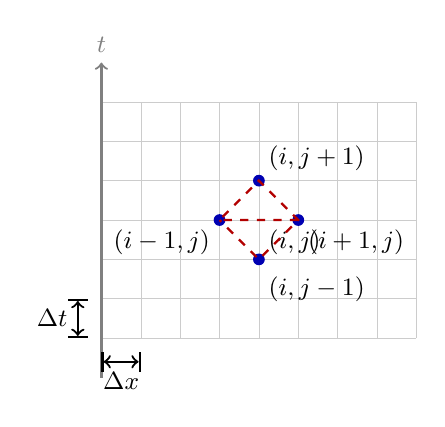
\begin{tikzpicture}[
  pde13grid/.style = {gray!40, very thin},
  pde13axis/.style = {->, thick, gray},
  pde13node/.style = {circle, fill=blue!70!black, inner sep=1.5pt},
  pde13center/.style = {circle, fill=red!70!black, inner sep=2pt},
  pde13lbl/.style = {font=\small}
]
  % 缃戞牸
  \foreach \x in {0,0.5,...,4} {
    \draw[pde13grid] (\x,0) -- (\x,3);
  }
  \foreach \y in {0,0.5,...,3} {
    \draw[pde13grid] (0,\y) -- (4,\y);
  }
  % 鏍囨敞缃戞牸鐐?  \node[pde13center] at (2, 1.5) {};
  \node[pde13lbl, below right] at (2, 1.5) {$(i,j)$};
  \node[pde13node] at (2.5, 1.5) {};
  \node[pde13lbl, below right] at (2.5, 1.5) {$(i+1,j)$};
  \node[pde13node] at (1.5, 1.5) {};
  \node[pde13lbl, below left] at (1.5, 1.5) {$(i-1,j)$};
  \node[pde13node] at (2, 2.0) {};
  \node[pde13lbl, above right] at (2, 2.0) {$(i,j+1)$};
  \node[pde13node] at (2, 1.0) {};
  \node[pde13lbl, below right] at (2, 0.9) {$(i,j-1)$};
  % 浜旂偣妯℃澘
  \draw[thick, red!70!black, dashed] (2.5,1.5) -- (1.5,1.5)
    -- (2,2.0) -- (2.5,1.5) -- (2,1.0) -- (1.5,1.5);
  % 鍧愭爣杞?  \draw[pde13axis] (-0.5,0) -- (4.5,0) node[right, pde13lbl] {$x$};
  \draw[pde13axis] (0,-0.5) -- (0,3.5) node[above, pde13lbl] {$t$};
  % 鏍囨敞姝ラ暱
  \draw[|<->|, thick] (0,-0.3) -- (0.5,-0.3)
    node[midway, below, pde13lbl] {$\Delta x$};
  \draw[|<->|, thick] (-0.3,0) -- (-0.3,0.5)
    node[midway, left, pde13lbl] {$\Delta t$};
\end{tikzpicture}
\caption{鏈夐檺宸垎娉曠殑缃戞牸涓庝簲鐐瑰樊鍒嗘ā鏉縸
\end{figure}

\begin{myexample}{涓€缁寸儹浼犲鏂圭▼鐨勬樉寮忓樊鍒嗘牸寮弣
鑰冭檻涓€缁寸儹浼犲鏂圭▼
\[
  \frac{\partial u}{\partial t} = \alpha\frac{\partial^2 u}{\partial x^2},
  \quad x \in [0,L],\; t > 0.
\]
鍒╃敤鏃堕棿鍓嶅悜宸垎鍜岀┖闂翠腑蹇冨樊鍒嗭紝寰楀埌\textbf{鏄惧紡宸垎鏍煎紡}锛圗xplicit Scheme锛夛細
\begin{equation}
  \frac{u_i^{n+1}-u_i^n}{\Delta t}
  = \alpha\frac{u_{i+1}^n-2u_i^n+u_{i-1}^n}{(\Delta x)^2},
  \label{eq:heat-explicit}
\end{equation}
鍏朵腑 $u_i^n \approx u(x_i, t_n)$锛?x_i = i\,\Delta x$锛?t_n = n\,\Delta t$銆傛暣鐞嗗緱
\[
  u_i^{n+1} = u_i^n + r\left(u_{i+1}^n - 2u_i^n + u_{i-1}^n\right),
  \quad r = \frac{\alpha\,\Delta t}{(\Delta x)^2}.
\]
\end{myexample}

\begin{myTheorem}{CFL 绋冲畾鎬ф潯浠秨
瀵逛簬涓€缁寸儹浼犲鏂圭▼鐨勬樉寮忓樊鍒嗘牸寮弤\eqref{eq:heat-explicit}锛屽綋
\begin{equation}
  r = \frac{\alpha\,\Delta t}{(\Delta x)^2} \leq \frac{1}{2}
  \label{eq:cfl-heat}
\end{equation}
鏃讹紝鏍煎紡鏄ǔ瀹氱殑锛涘綋 $r > 1/2$ 鏃讹紝鏍煎紡涓嶇ǔ瀹氾紝鏁板€艰В浼氬嚭鐜版尟鑽″苟瓒嬩簬鏃犵┓銆?\end{myTheorem}

\begin{myremark}
CFL 鏉′欢锛圕ourant--Friedrichs--Lewy Condition锛夋槸鏁板€兼眰瑙ｅ亸寰垎鏂圭▼鐨勫熀鏈ǔ瀹氭€ф潯浠躲€傚浜庢尝鍔ㄦ柟绋嬶紝CFL 鏉′欢涓?$c\,\Delta t / \Delta x \leq 1$锛屽叾涓?$c$ 鏄尝閫熴€侰FL 鏉′欢鐨勭墿鐞嗗惈涔夋槸锛氭暟鍊间俊鎭殑浼犳挱閫熷害蹇呴』涓嶅皬浜庣墿鐞嗕俊鎭殑浼犳挱閫熷害銆?\end{myremark}

\begin{figure}[htbp]
\centering
\begin{tikzpicture}[
  pde13exact/.style = {thick, blue!70!black},
  pde13stable/.style = {thick, red!70!black, dashed},
  pde13unstable/.style = {thick, orange!80!black, dashdotted},
  pde13axis/.style = {->, thick, gray},
  pde13lbl/.style = {font=\small}
]
  % 鍧愭爣杞?  \draw[pde13axis] (-0.3,0) -- (6.5,0) node[right, pde13lbl] {$x$};
  \draw[pde13axis] (0,-0.5) -- (0,1.5) node[above, pde13lbl] {$u$};
  % 绮剧‘瑙ｏ紙楂樻柉鍒嗗竷鐨勮“鍑忥級
  \draw[pde13exact, domain=0:6.3, samples=200]
    plot (\x, {1.0*exp(-(\x-3.15)^2/0.8)});
  \node[pde13exact, right, pde13lbl] at (6.5, 1.2) {绮剧‘瑙;
  % 绋冲畾鏁板€艰В (r=0.4)
  \draw[pde13stable, domain=0.3:6, samples=20]
    plot (\x, {0.92*exp(-(\x-3.15)^2/0.9)
    + 0.03*sin(deg(\x*100))});
  \node[pde13stable, right, pde13lbl] at (6.5, 0.9) {绋冲畾锛?r=0.4$锛墋;
  % 涓嶇ǔ瀹氭暟鍊艰В (r=0.6)
  \draw[pde13unstable, domain=0.3:6, samples=20]
    plot (\x, {0.8*exp(-(\x-3.15)^2/1.0)
    + 0.3*sin(deg(\x*100))});
  \node[pde13unstable, right, pde13lbl] at (6.5, 0.5) {涓嶇ǔ瀹氾紙$r=0.6$锛墋;
  % 鏍囨敞
  \node[pde13lbl] at (3, -0.3) {鐑紶瀵兼柟绋嬫樉寮忔牸寮忕殑绋冲畾鎬у姣攠;
\end{tikzpicture}
\caption{鏄惧紡宸垎鏍煎紡鍦ㄤ笉鍚?$r$ 鍊间笅鐨勭ǔ瀹氭€у姣攠
\end{figure}

%% ============================================================
\section{鏈夐檺鍏冩硶绠€浠媫

\begin{mydefinition}{鏈夐檺鍏冩硶}
\textbf{鏈夐檺鍏冩硶}锛團inite Element Method, FEM锛夋槸涓€绉嶅熀浜庡彉鍒嗗師鐞嗙殑鏁板€兼柟娉曘€傚叾鍩烘湰鎬濇兂鏄細
\begin{enumerate}
  \item 灏嗗亸寰垎鏂圭▼鍖栦负寮卞舰寮忥紙绉垎褰㈠紡锛夛紱
  \item 灏嗘眰瑙ｅ尯鍩熷垝鍒嗕负鑻ュ共灏忕殑鍗曞厓锛坋lement锛夛紱
  \item 鍦ㄦ瘡涓崟鍏冧笂鐢ㄧ畝鍗曠殑澶氶」寮忓嚱鏁帮紙褰㈠嚱鏁帮級杩戜技瑙ｏ紱
  \item 缁勮鎴愬叧浜庤妭鐐瑰€肩殑绾挎€ф柟绋嬬粍骞舵眰瑙ｃ€?\end{enumerate}
\end{mydefinition}

鏈夐檺鍏冩硶鐨勬牳蹇冧紭鍔垮湪浜庯細
\begin{itemize}
  \item 鑳藉澶勭悊澶嶆潅鐨勫嚑浣曞舰鐘跺拰涓嶈鍒欒竟鐣岋紱
  \item 渚夸簬澶勭悊娣峰悎杈圭晫鏉′欢锛圖irichlet 鍜?Neumann 鏉′欢鐨勭粍鍚堬級锛?  \item 鏈夌郴缁熺殑璇樊鍒嗘瀽鐞嗚锛?h$-缁嗗寲鍜?$p$-缁嗗寲锛夛紱
  \item 宸叉湁澶ч噺鎴愮啛鐨勮蒋浠跺寘锛堝 FEniCS銆丗reeFEM++銆丆OMSOL 绛夛級銆?\end{itemize}

鏈夐檺鍏冩硶鐨勫疄鏂芥楠ゅ彲浠ユ鎷负锛?
\begin{figure}[htbp]
\centering
\begin{tikzpicture}[
  pde13flow/.style = {rectangle, draw=blue!70!black, rounded corners,
    minimum width=2.8cm, minimum height=0.7cm, text centered,
    font=\small, fill=blue!8},
  pde13arr/.style = {->, >=stealth, thick, blue!70!black}
]
  \node[pde13flow] (A) at (0,0) {寤虹珛 PDE 妯″瀷};
  \node[pde13flow] (B) at (0,-1.5) {鎺ㄥ寮卞舰寮弣;
  \node[pde13flow] (C) at (0,-3.0) {鍖哄煙鍓栧垎};
  \node[pde13flow] (D) at (0,-4.5) {鏋勯€犲舰鍑芥暟};
  \node[pde13flow] (E) at (0,-6.0) {鍗曞厓鍒氬害鐭╅樀};
  \node[pde13flow] (F) at (0,-7.5) {鍏ㄥ眬缁勮};
  \node[pde13flow] (G) at (0,-9.0) {鏂藉姞杈圭晫鏉′欢};
  \node[pde13flow] (H) at (0,-10.5) {姹傝В绾挎€ф柟绋嬬粍};

  \draw[pde13arr] (A) -- (B);
  \draw[pde13arr] (B) -- (C);
  \draw[pde13arr] (C) -- (D);
  \draw[pde13arr] (D) -- (E);
  \draw[pde13arr] (E) -- (F);
  \draw[pde13arr] (F) -- (G);
  \draw[pde13arr] (G) -- (H);
\end{tikzpicture}
\caption{鏈夐檺鍏冩硶鐨勫疄鏂芥祦绋媫
\end{figure}

\begin{myexample}{Poisson 鏂圭▼鐨勬湁闄愬厓绂绘暎}
鑰冭檻 Poisson 鏂圭▼ $-\Delta u = f$ 鍦ㄥ尯鍩?$\Omega$ 涓婏紝$u|_{\partial\Omega}=0$銆?
寮卞舰寮忥細姹?$u \in H_0^1(\Omega)$ 浣垮緱
\[
  \int_\Omega \nabla u \cdot \nabla v\,dx = \int_\Omega f\,v\,dx,
  \quad \forall v \in H_0^1(\Omega).
\]
灏?$u \approx u_h = \sum_{j=1}^{N} c_j \phi_j$锛?\phi_j$ 涓烘湁闄愬厓鍩哄嚱鏁帮級锛屽緱鍒扮嚎鎬ф柟绋嬬粍
\[
  \mathbf{K}\,\mathbf{c} = \mathbf{f},
\]
鍏朵腑 $K_{ij} = \int_\Omega \nabla\phi_i \cdot \nabla\phi_j\,dx$ 鏄垰搴︾煩闃碉紙Stiffness Matrix锛夛紝$f_i = \int_\Omega f\,\phi_i\,dx$ 鏄嵎杞藉悜閲忋€?\end{myexample}

\begin{myremark}
鏈夐檺鍏冩硶涓庡彉鍒嗘硶鐨?Rayleigh--Ritz 鏂规硶鏈川涓婃槸涓€鑷寸殑锛屽尯鍒湪浜庢湁闄愬厓娉曚娇鐢ㄥ垎鐗囧椤瑰紡浣滀负鍩哄嚱鏁帮紝杩欎娇寰楀畠鑳藉鐏垫椿鍦板鐞嗗鏉傚嚑浣曞舰鐘躲€傛湁闄愬厓鏂规硶鍦ㄧ粨鏋勫姏瀛︺€佺儹浼犲銆佺數纾佸満浠跨湡绛夐鍩熸湁鏋佷负骞挎硾鐨勫簲鐢ㄣ€?\end{myremark}

%% ============================================================
\section{璋辨柟娉晑

\begin{mydefinition}{璋辨柟娉晑
\textbf{璋辨柟娉晑锛圫pectral Method锛夋槸鐢ㄥ叏灞€鍩哄嚱鏁帮紙濡?Fourier 绾ф暟鎴?Chebyshev 澶氶」寮忥級鐨勬湁闄愭埅鏂潵杩戜技鍋忓井鍒嗘柟绋嬬殑瑙ｇ殑鏂规硶銆傚叾鍩烘湰鎬濇兂鏄細
\begin{enumerate}
  \item 灏嗚В灞曞紑涓哄叏灞€鍩哄嚱鏁扮殑鏈夐檺鍜岋細$u_N(x) = \sum_{k=0}^{N} \hat{u}_k\,\phi_k(x)$锛?  \item 灏嗗睍寮€寮忎唬鍏ュ亸寰垎鏂圭▼锛屽埄鐢?Galerkin 鏉′欢鎴栭厤缃偣鏉′欢纭畾绯绘暟 $\hat{u}_k$銆?\end{enumerate}
\end{mydefinition}

璋辨柟娉曞彲鍒嗕负涓夌绫诲瀷锛?\begin{itemize}
  \item \textbf{Fourier 璋辨柟娉晑锛氶€傜敤浜庡懆鏈熼棶棰橈紝鍩哄嚱鏁颁负 $e^{ikx}$锛?  \item \textbf{Chebyshev 璋辨柟娉晑锛氶€傜敤浜庨潪鍛ㄦ湡闂锛屽熀鍑芥暟涓?Chebyshev 澶氶」寮?$T_n(x)$锛?  \item \textbf{Legendre 璋辨柟娉晑锛氬熀鍑芥暟涓?Legendre 澶氶」寮?$P_n(x)$銆?\end{itemize}

\begin{myTheorem}{璋辨柟娉曠殑绮惧害}
瀵逛簬瓒冲鍏夋粦鐨勮В锛岃氨鏂规硶鐨勮宸互\textbf{鎸囨暟閫熷害}鏀舵暃锛堣氨绮惧害锛孲pectral Accuracy锛夛細
\[
  \|u - u_N\| \leq C\,e^{-cN},
\]
鍏朵腑 $C, c > 0$ 鏄笌 $N$ 鏃犲叧鐨勫父鏁般€傝繖杩滀紭浜庢湁闄愬樊鍒嗘硶鍜屾湁闄愬厓娉曠殑浠ｆ暟鏀舵暃閫熷害 $O(h^p)$銆?\end{myTheorem}

\begin{myremark}
璋辨柟娉曠殑浼樺娍鍦ㄤ簬瀵瑰厜婊戦棶棰樺叿鏈夋瀬楂樼殑绮惧害锛屽彲浠ョ敤杈冨皯鐨勮嚜鐢卞害杈惧埌寰堥珮鐨勭簿搴︺€傜己鐐规槸瀵逛笉鍏夋粦瑙ｏ紙濡傛湁闂存柇鐨勮В锛夋晥鏋滆緝宸紝涓旈渶瑕佸叏灞€鍩哄嚱鏁帮紝涓嶅鏈夐檺鍏冩硶鐏垫椿銆傚湪姘斿€欐ā鎷燂紙璋辨柟娉曞ぇ姘旀ā寮忥級銆佹箥娴佺洿鎺ユ暟鍊兼ā鎷燂紙DNS锛夌瓑棰嗗煙锛岃氨鏂规硶鏈夐噸瑕佸簲鐢ㄣ€?\end{myremark}

\begin{figure}[htbp]
\centering
\begin{tikzpicture}[
  pde13exact/.style = {thick, blue!70!black},
  pde13spec4/.style = {thick, red!70!black, dashed},
  pde13spec8/.style = {thick, green!50!black, dashdotted},
  pde13axis/.style = {->, thick, gray},
  pde13lbl/.style = {font=\small}
]
  % 鍧愭爣杞?  \draw[pde13axis] (-0.5,0) -- (6.5,0) node[right, pde13lbl] {$x$};
  \draw[pde13axis] (0,-1.5) -- (0,1.5) node[above, pde13lbl] {};
  % 绮剧‘瑙?  \draw[pde13exact, domain=0:6.28, samples=200]
    plot (\x, {sin(deg(\x)) + 0.3*sin(deg(3*\x))});
  \node[pde13exact, right, pde13lbl] at (6.3, 1.2) {绮剧‘瑙;
  % 璋辫繎浼硷紙N=4锛?  \draw[pde13spec4, domain=0:6.28, samples=200]
    plot (\x, {sin(deg(\x)) + 0.28*sin(deg(3*\x))
    + 0.02*sin(deg(5*\x))});
  \node[pde13spec4, right, pde13lbl] at (6.3, 0.7) {$N=4$ 璋辫繎浼紏;
  % 璋辫繎浼硷紙N=8锛?  \draw[pde13spec8, domain=0:6.28, samples=200]
    plot (\x, {sin(deg(\x)) + 0.3*sin(deg(3*\x))});
  \node[pde13spec8, right, pde13lbl] at (6.3, 0.2) {$N=8$ 璋辫繎浼硷紙鍑犱箮閲嶅悎锛墋;
  % 鏍囨敞
  \node[pde13lbl] at (3.14, -1.3) {璋辨柟娉曚互鎸囨暟閫熷害鏀舵暃鍒扮簿纭В};
\end{tikzpicture}
\caption{璋辨柟娉曞鍏夋粦鍑芥暟鐨勯€艰繎鏁堟灉}
\end{figure}

%% ============================================================
\section{鏁板€肩ǔ瀹氭€у垎鏋恾

\begin{mydefinition}{鏁板€肩ǔ瀹氭€
璁?$\mathbf{u}^n$ 涓烘暟鍊艰В鍦ㄧ $n$ 姝ョ殑鍊笺€傚鏋滃瓨鍦ㄥ父鏁?$C > 0$ 浣垮緱
\[
  \|\mathbf{u}^n\| \leq C\,\|\mathbf{u}^0\|, \quad \forall n \geq 0,
\]
鍒欑О璇ユ暟鍊兼牸寮忔槸\textbf{绋冲畾鐨剗锛圫table锛夈€傚惁鍒欑О涓轰笉绋冲畾鐨勩€?\end{mydefinition}

鍒嗘瀽鏁板€肩ǔ瀹氭€х殑涓昏鏂规硶鏈夛細

\begin{myTheorem}{Von Neumann 绋冲畾鎬у垎鏋恾
鑰冭檻绾挎€у父绯绘暟宸垎鏂圭▼锛岃瑙ｇ殑褰㈠紡涓?$\hat{u}^n\,e^{ikx}$锛屽叾涓?$\hat{u}^n$ 鏄 $n$ 姝ョ殑鎸箙銆傚畾涔塡textbf{鏀惧ぇ鍥犲瓙}锛圓mplification Factor锛?\[
  G(k) = \frac{\hat{u}^{n+1}}{\hat{u}^n}.
\]
Von Neumann 绋冲畾鎬ф潯浠惰姹?\begin{equation}
  |G(k)| \leq 1, \quad \forall k.
  \label{eq:von-neumann}
\end{equation}
\end{myTheorem}

\begin{myexample}{鏄惧紡鏍煎紡鐨?Von Neumann 鍒嗘瀽}
瀵逛竴缁寸儹浼犲鏂圭▼鐨勬樉寮忔牸寮忥紝璁?$u_i^n = G^n\,e^{ik(i\Delta x)}$锛屼唬鍏ュ樊鍒嗘牸寮忓緱
\[
  G = 1 - 4r\sin^2\!\left(\frac{k\Delta x}{2}\right),
\]
鍏朵腑 $r = \alpha\,\Delta t/(\Delta x)^2$銆傝姹?$|G| \leq 1$锛屽嵆
\[
  -1 \leq 1 - 4r\sin^2\!\left(\frac{k\Delta x}{2}\right) \leq 1.
\]
鍙宠竟鐨勪笉绛夊紡鎬绘槸鎴愮珛锛屽乏杈硅姹?$4r\sin^2(k\Delta x/2) \leq 2$锛屽嵆 $r \leq 1/2$銆?\end{myexample}

\begin{myremark}
Von Neumann 鍒嗘瀽鏄ǔ瀹氭€у垎鏋愮殑鍩烘湰宸ュ叿锛屼絾浠呴€傜敤浜庣嚎鎬у父绯绘暟闂鍜屽懆鏈熻竟鐣屾潯浠躲€傚浜庢洿涓€鑸殑鎯呭喌锛岄渶瑕佷娇鐢ㄨ兘閲忔柟娉曪紙Energy Method锛夋垨鐭╅樀鏂规硶杩涜鍒嗘瀽銆傚浜庨潪绾挎€ф柟绋嬶紝绋冲畾鎬у垎鏋愭洿鍔犲鏉傦紝閫氬父闇€瑕佺粨鍚堝叿浣撻棶棰樿繘琛岀壒娈婂鐞嗐€?\end{myremark}

%% ============================================================
\section{Python 瀹炵幇绀轰緥}

\begin{lstlisting}[language=Python, caption={鏈夐檺宸垎娉曟眰瑙ｄ竴缁寸儹浼犲鏂圭▼}]
import numpy as np
import matplotlib.pyplot as plt

# 鍙傛暟璁剧疆
L = 1.0       # 鏉嗛暱
alpha = 0.01  # 鐑墿鏁ｇ郴鏁?T = 2.0       # 鎬绘椂闂?Nx = 50       # 绌洪棿缃戞牸鏁?dx = L / Nx
x = np.linspace(0, L, Nx + 1)

# 绋冲畾鎬ф潯浠讹細r <= 0.5
r = 0.4
dt = r * dx**2 / alpha
Nt = int(T / dt)
print(f"r = {r}, dt = {dt:.6f}, Nt = {Nt}")

# 鍒濆鏉′欢锛氭寮﹀垎甯?u = np.sin(np.pi * x)

# 杈圭晫鏉′欢锛歶(0,t) = u(L,t) = 0
# 鏃堕棿鎺ㄨ繘锛堟樉寮忔牸寮忥級
u_history = [u.copy()]
for n in range(Nt):
    u_new = u.copy()
    for i in range(1, Nx):
        u_new[i] = u[i] + r * (u[i+1] - 2*u[i] + u[i-1])
    u_new[0] = 0.0
    u_new[Nx] = 0.0
    u = u_new
    if (n+1) % (Nt // 10) == 0:
        u_history.append(u.copy())

# 绮剧‘瑙?u_exact = np.sin(np.pi * x) * np.exp(-alpha * np.pi**2 * T)

# 缁樺浘
fig, ax = plt.subplots(figsize=(10, 5))
for i, u_snap in enumerate(u_history):
    t_val = i * (Nt // 10) * dt
    ax.plot(x, u_snap, label=f't={t_val:.2f}', alpha=0.7)
ax.plot(x, u_exact, 'k--', linewidth=2, label='绮剧‘瑙?(t=2.0)')
ax.set_xlabel('$x$', fontsize=12)
ax.set_ylabel('$u(x,t)$', fontsize=12)
ax.set_title(f'鏈夐檺宸垎娉曟眰瑙ｇ儹浼犲鏂圭▼ ($r={r}$)', fontsize=14)
ax.legend(fontsize=10)
ax.grid(True, alpha=0.3)
plt.tight_layout()
plt.show()
\end{lstlisting}

\begin{myexample}{鏈夐檺鍏冩硶姹傝В Poisson 鏂圭▼}
涓嬮潰缁欏嚭浣跨敤 FEniCS 搴撴眰瑙ｄ竴缁?Poisson 鏂圭▼鐨勭ず渚嬫鏋躲€?
\begin{lstlisting}[language=Python, caption={鏈夐檺鍏冩硶姹傝В Poisson 鏂圭▼锛團EniCS 妗嗘灦锛墋]
# 闇€瑕佸畨瑁? pip install fenics-dolfinx
import numpy as np
import matplotlib.pyplot as plt
from scipy.sparse import diags
from scipy.sparse.linalg import spsolve

# 涓€缁?Poisson 鏂圭▼: -u'' = f(x), u(0)=u(1)=0
# 鏈夐檺鍏冪鏁ｏ紙绾挎€у厓锛?=> 涓夊瑙掑垰搴︾煩闃?
N = 100  # 鍗曞厓鏁?h = 1.0 / N
x = np.linspace(0, 1, N + 1)

# 鑽疯浇鍚戦噺锛歠(x) = pi^2 * sin(pi*x) => 绮剧‘瑙?u = sin(pi*x)
f_vals = np.pi**2 * np.sin(np.pi * x[1:-1])

# 鏈夐檺鍏冨垰搴︾煩闃碉紙涓€缁寸嚎鎬у厓锛?# K_ij = int(phi_i' phi_j' dx)
main_diag = 2.0 / h * np.ones(N - 1)
off_diag = -1.0 / h * np.ones(N - 2)
K = diags([off_diag, main_diag, off_diag], [-1, 0, 1],
          format='csc')

# 鑽疯浇鍚戦噺
F = f_vals * h  # 姊舰鍏紡

# 姹傝В
u_interior = spsolve(K, F)
u_fem = np.zeros(N + 1)
u_fem[1:-1] = u_interior

# 绮剧‘瑙?u_exact = np.sin(np.pi * x)

# 缁樺浘瀵规瘮
fig, ax = plt.subplots(figsize=(10, 5))
ax.plot(x, u_fem, 'ro-', markersize=3, label='鏈夐檺鍏冭В')
ax.plot(x, u_exact, 'b-', linewidth=2, label='绮剧‘瑙?)
ax.set_xlabel('$x$', fontsize=12)
ax.set_ylabel('$u(x)$', fontsize=12)
ax.set_title('鏈夐檺鍏冩硶姹傝В涓€缁?Poisson 鏂圭▼', fontsize=14)
ax.legend(fontsize=11)
ax.grid(True, alpha=0.3)
plt.tight_layout()
plt.show()
\end{lstlisting}
\end{myexample}

\begin{figure}[htbp]
\centering
\begin{tikzpicture}[
  pde13fem/.style = {thick, draw=blue!70!black},
  pde13node/.style = {circle, fill=blue!70!black, inner sep=1.2pt},
  pde13axis/.style = {->, thick, gray},
  pde13lbl/.style = {font=\small}
]
  % 涓€缁寸綉鏍?  \foreach \x in {0,0.5,...,4} {
    \draw[pde13fem] (\x,0) -- (\x+0.5,0);
    \node[pde13node] at (\x,0) {};
  }
  \node[pde13node] at (4.5,0) {};
  % 鑺傜偣缂栧彿
  \node[pde13lbl, below] at (0,0) {$x_0$};
  \node[pde13lbl, below] at (0.5,0) {$x_1$};
  \node[pde13lbl, below] at (1.0,0) {$x_2$};
  \node[pde13lbl, below] at (3.5,0) {$x_{N-1}$};
  \node[pde13lbl, below] at (4.0,0) {$x_N$};
  % 褰㈠嚱鏁扮ず鎰?  \draw[thick, red!70!black] (0.5,0) -- (1.0,1.2) -- (1.5,0);
  \node[pde13lbl, red!70!black, above] at (1.0, 1.3) {$\phi_2(x)$};
  % 涓夊瑙掔煩闃电ず鎰?  \node[pde13lbl] at (2.25, -1.0)
    {涓夊瑙掑垰搴︾煩闃碉細$\mathbf{K} = \frac{1}{h}\text{tridiag}(-1,2,-1)$};
\end{tikzpicture}
\caption{鏈夐檺鍏冩硶鐨勪竴缁寸嚎鎬у舰鍑芥暟涓庝笁瀵硅鍒氬害鐭╅樀}
\end{figure}

\begin{myremark}
鍦ㄥ疄闄呭簲鐢ㄤ腑锛屾湁闄愬厓娉曢€氬父澶勭悊浜岀淮鍜屼笁缁撮棶棰樸€備簩缁撮棶棰樹腑甯哥敤鐨勫崟鍏冩湁涓夎褰㈠崟鍏冨拰鍥涜竟褰㈠崟鍏冿紝涓夌淮闂涓湁鍥涢潰浣撳崟鍏冨拰鍏潰浣撳崟鍏冦€傜幇浠ｆ湁闄愬厓杞欢鍙互鑷姩瀹屾垚缃戞牸鐢熸垚銆佺煩闃电粍瑁呭拰鍚庡鐞嗙瓑宸ヤ綔銆?\end{myremark}

%% ============================================================
\section*{鏈珷灏忕粨}

鏈珷浠嬬粛浜嗗亸寰垎鏂圭▼鏁板€艰В娉曠殑涓夊ぇ涓绘祦鏂规硶锛?\begin{itemize}
  \item \textbf{鏈夐檺宸垎娉晑锛氱畝鍗曠洿瑙傦紝閫傜敤浜庤鍒欏尯鍩熴€傛牳蹇冩蹇垫槸宸垎鏍煎紡鍜岀ǔ瀹氭€ф潯浠讹紙CFL 鏉′欢锛夛紱
  \item \textbf{鏈夐檺鍏冩硶}锛氬熀浜庡彉鍒嗗師鐞嗭紝閫傜敤浜庡鏉傚嚑浣曘€傛牳蹇冩楠ゆ槸寮卞舰寮忔帹瀵笺€佺綉鏍煎墫鍒嗗拰鍒氬害鐭╅樀缁勮锛?  \item \textbf{璋辨柟娉晑锛氬埄鐢ㄥ叏灞€鍩哄嚱鏁帮紝瀵瑰厜婊戦棶棰樻湁鎸囨暟鏀舵暃閫熷害銆傞€傚悎鍛ㄦ湡闂鍜屽厜婊戣В锛?  \item \textbf{鏁板€肩ǔ瀹氭€锛歏on Neumann 鍒嗘瀽鏄垽鏂樊鍒嗘牸寮忕ǔ瀹氭€х殑鍩烘湰宸ュ叿锛?  \item 閫夋嫨鍚堥€傜殑鏁板€兼柟娉曢渶瑕佺患鍚堣€冭檻闂鐨勫嚑浣曘€佽В鐨勫厜婊戞€у拰绮惧害瑕佹眰銆?\end{itemize}

%% ============================================================
\section*{缁冧範棰榼

\begin{enumerate}
  \item 瀵逛竴缁存尝鍔ㄦ柟绋?$u_{tt} = c^2 u_{xx}$ 鎺ㄥ鏄惧紡宸垎鏍煎紡锛屽苟鍒嗘瀽鍏?CFL 绋冲畾鎬ф潯浠躲€?
  \item 鐢?Python 瀹炵幇鏈夐檺宸垎娉曟眰瑙ｄ竴缁寸儹浼犲鏂圭▼锛屽彇 $r = 0.6$锛堣秴杩囩ǔ瀹氭€ф潯浠讹級锛岃瀵熸暟鍊艰В鐨勪笉绋冲畾鐜拌薄銆?
  \item 瀵逛竴缁?Poisson 鏂圭▼ $-u'' = 2$锛?u(0)=u(1)=0$锛夛紝鐢ㄦ湁闄愬厓娉曪紙绾挎€у厓锛夋帹瀵煎垰搴︾煩闃靛拰鑽疯浇鍚戦噺锛屽苟姹傝В涓庣簿纭В $u = x(1-x)$ 姣旇緝銆?
  \item 鐢?Fourier 璋辨柟娉曡繎浼煎嚱鏁?$f(x) = \sin(x) + 0.5\sin(3x)$锛屽垎鍒彇 $N=2$ 鍜?$N=6$锛岀粯鍒惰繎浼兼洸绾垮苟涓庣簿纭В姣旇緝銆?
  \item 涓轰粈涔堟湁闄愬厓娉曟瘮鏈夐檺宸垎娉曟洿閫傚悎澶勭悊澶嶆潅鍑犱綍褰㈢姸锛熶粠鍩哄嚱鏁扮殑閫夋嫨鍜岀綉鏍肩伒娲绘€т袱涓搴﹁璁恒€?\end{enumerate}

\chapter{搴旂敤瀹炰緥}

\section*{寮曡█}

鏈珷灏嗗墠闈㈠悇绔犲涔犵殑鏁板鐗╃悊鏂圭▼鐞嗚搴旂敤浜庝簲涓吀鍨嬬殑鐗╃悊闂锛氬鸡鎸姩闂銆佺儹浼犲闂銆佺數纾佸満闂銆侀噺瀛愬姏瀛︿腑鐨勫簲鐢ㄤ互鍙婃祦浣撳姏瀛︿腑鐨勫簲鐢ㄣ€傝繖浜涘疄渚嬪睍绀轰簡鍋忓井鍒嗘柟绋嬬悊璁哄浣曟弿杩板拰瑙ｅ喅瀹為檯鐨勭墿鐞嗛棶棰橈紝涔熶綋鐜颁簡涓嶅悓鐗╃悊棰嗗煙涔嬮棿鐨勬暟瀛︾粺涓€鎬с€?
姣忎釜瀹炰緥閮藉寘鍚細鐗╃悊鑳屾櫙鐨勪粙缁嶃€佹暟瀛︽ā鍨嬬殑寤虹珛銆佹眰瑙ｈ繃绋嬶紙瑙ｆ瀽鎴栨暟鍊硷級浠ュ強缁撴灉鐨勭墿鐞嗚В閲娿€傞€氳繃杩欎簺瀹炰緥锛岃鑰呭彲浠ョ湅鍒版暟瀛︾墿鐞嗘柟绋嬩笉浠呮槸鎶借薄鐨勬暟瀛︾悊璁猴紝鏇存槸鐞嗚В鑷劧鐜拌薄鍜岃В鍐冲伐绋嬮棶棰樼殑鏈夊姏宸ュ叿銆?
\begin{myremark}
鏁板鐗╃悊鏂圭▼鐨勬牳蹇冧环鍊煎湪浜庯細涓嶅悓鐨勭墿鐞嗙幇璞★紙寮︽尟鍔ㄣ€佺儹浼犲銆佺數纾佹尝锛夊彲浠ョ敤鐩稿悓鎴栫浉浼肩殑鍋忓井鍒嗘柟绋嬫潵鎻忚堪銆傝繖绉嶆暟瀛︿笂鐨勭粺涓€鎬т娇寰楁垜浠彲浠ュ皢鍦ㄤ竴涓鍩熷彂灞曞嚭鏉ョ殑姹傝В鏂规硶绉绘鍒板彟涓€涓鍩燂紝杩欎篃鏄暟瀛︾墿鐞嗘柟娉曠殑寮哄ぇ涔嬪銆?\end{myremark}

%% ============================================================
\section{寮︽尟鍔ㄩ棶棰榼

\begin{mydefinition}{寮︽尟鍔ㄦ柟绋媫
涓€鏍归暱搴︿负 $L$ 鐨勭悊鎯冲鸡锛堜笉鍙几闀裤€佹棤寮规€с€佹棤鎽╂摝锛夛紝鍦ㄥ紶鍔?$T$ 鍜岀嚎瀵嗗害 $\rho$ 鐨勪綔鐢ㄤ笅鍋氭í鍚戝井灏忔尟鍔ㄣ€傝浣嶇Щ涓?$u(x,t)$锛屽垯 $u$ 婊¤冻涓€缁存尝鍔ㄦ柟绋嬶細
\begin{equation}
  \frac{\partial^2 u}{\partial t^2} = c^2\frac{\partial^2 u}{\partial x^2},
  \quad x \in [0,L],\; t > 0,
  \label{eq:string-wave}
\end{equation}
鍏朵腑 $c = \sqrt{T/\rho}$ 鏄尝閫熴€?\end{mydefinition}

\begin{myexample}{鍥哄畾绔鸡鐨勮嚜鐢辨尟鍔▆
涓ょ鍥哄畾鐨勫鸡锛?u(0,t)=u(L,t)=0$锛夛紝鍒濆浣嶇Щ涓?$u(x,0) = f(x)$锛屽垵濮嬮€熷害涓?$u_t(x,0) = g(x)$銆傚埄鐢ㄥ垎绂诲彉閲忔硶锛岃В涓?\begin{equation}
  u(x,t) = \sum_{n=1}^{\infty}\left(A_n\cos\frac{n\pi ct}{L}
  + B_n\sin\frac{n\pi ct}{L}\right)\sin\frac{n\pi x}{L},
  \label{eq:string-solution}
\end{equation}
鍏朵腑
\[
  A_n = \frac{2}{L}\int_0^L f(x)\sin\frac{n\pi x}{L}\,dx, \quad
  B_n = \frac{2}{n\pi c}\int_0^L g(x)\sin\frac{n\pi x}{L}\,dx.
\]
\end{myexample}

寮︾殑鎸姩鍙互鍒嗚В涓哄悇闃舵ā鎬佺殑鍙犲姞銆傜 $n$ 闃舵ā鎬佸搴旂殑棰戠巼涓?\[
  f_n = \frac{nc}{2L} = \frac{n}{2L}\sqrt{\frac{T}{\rho}},
\]
鍩洪 $f_1$ 瀵瑰簲寮﹀彂鍑虹殑鏈€浣庨煶璋冿紝$f_n = nf_1$ 涓虹 $n$ 娆¤皭娉€?
\begin{figure}[htbp]
\centering
\begin{tikzpicture}[
  pde14string/.style = {thick, blue!70!black},
  pde14mode/.style = {thick},
  pde14axis/.style = {->, thick, gray},
  pde14node/.style = {circle, fill=black, inner sep=1.5pt},
  pde14lbl/.style = {font=\small}
]
  % 寮︾殑绀烘剰鍥撅紙鍒濆浣嶇Щ锛?  \draw[pde14string, domain=0:8, samples=200]
    plot (\x, {1.2*sin(deg(pi*\x/8))*exp(-0.05*\x)});
  \node[pde14string, right, pde14lbl] at (8.2, 0.8) {寮︾殑褰㈢姸};
  % 鍥哄畾绔?  \node[pde14node] at (0,0) {};
  \node[pde14node] at (8,0) {};
  \draw[thick] (-0.3,-0.3) -- (0.3,-0.3) -- (0,0.1) -- cycle;
  \draw[thick] (7.7,-0.3) -- (8.3,-0.3) -- (8,0.1) -- cycle;
  % 寮犲姏绠ご
  \draw[->, thick, red!70!black] (4, 0.5) -- (6, 0.8)
    node[midway, above, pde14lbl] {$T$};
  \draw[->, thick, red!70!black] (4, 0.5) -- (2, 0.8)
    node[midway, above, pde14lbl] {$T$};
  % 妯℃€?  \foreach \n/\clr/\yshift in {1/blue!70!black/3, 2/red!70!black/5, 3/green!50!black/7} {
    \draw[thick, \clr, domain=0:8, samples=200, shift={(0,\yshift)}]
      plot (\x, {0.6*sin(deg(\n*pi*\x/8))});
    \node[pde14lbl, \clr, right] at (8.2, \yshift)
      {绗?\n 闃舵ā鎬?($f_{\n}=\n f_1$)};
    \node[pde14node] at (0,\yshift) {};
    \node[pde14node] at (8,\yshift) {};
  }
  % 鍧愭爣杞?  \draw[pde14axis] (-0.5,0) -- (9,0);
  \draw[pde14axis] (-0.5,0) -- (-0.5,8.5) node[above, pde14lbl] {};
\end{tikzpicture}
\caption{寮︽尟鍔ㄧ殑鍓嶄笁闃舵ā鎬亇
\end{figure}

\begin{lstlisting}[language=Python, caption={寮︽尟鍔ㄧ殑杈炬湕璐濆皵瑙ｄ笌妯℃€佸彔鍔爙]
import numpy as np
import matplotlib.pyplot as plt
from matplotlib.animation import FuncAnimation

# 杈炬湕璐濆皵瑙?L = 1.0   # 寮﹂暱
c = 1.0   # 娉㈤€?Nx = 200  # 绌洪棿缃戞牸
x = np.linspace(0, L, Nx + 1)

# 鍒濆浣嶇Щ: 涓夎褰㈣剦鍐?def f(x):
    """鍒濆浣嶇Щ"""
    return np.where(x < L/2, 2*x/L, 2*(L-x)/L)

# 杈炬湕璐濆皵瑙? u(x,t) = [f(x+ct) + f(x-ct)] / 2
# 锛堟棤鍒濆閫熷害鎯呭舰锛?fig, ax = plt.subplots(figsize=(10, 5))
t_values = [0.0, 0.1, 0.2, 0.3, 0.4]

for t in t_values:
    u = 0.5 * (np.clip(f(x + c*t), 0, 1)
             + np.clip(f(x - c*t), 0, 1))
    ax.plot(x, u, label=f't={t:.1f}', linewidth=2)

ax.set_xlabel('$x/L$', fontsize=12)
ax.set_ylabel('$u(x,t)$', fontsize=12)
ax.set_title('杈炬湕璐濆皵瑙ｏ細寮︿笂涓夎褰㈣剦鍐茬殑浼犳挱', fontsize=14)
ax.legend(fontsize=11)
ax.grid(True, alpha=0.3)
ax.set_ylim(0, 1.1)
plt.tight_layout()
plt.show()
\end{lstlisting}

\begin{myremark}
寮︽尟鍔ㄩ棶棰樻槸鍘嗗彶涓婄涓€涓涓ユ牸姹傝В鐨勫亸寰垎鏂圭▼闂锛坉'Alembert, 1747锛夈€傚畠鐨勬眰瑙ｆ帹鍔ㄤ簡 Fourier 鍒嗘瀽鐨勮癁鐢燂紝涔熷紩鍙戜簡鍏充簬鍋忓井鍒嗘柟绋嬭В鐨勫瓨鍦ㄦ€у拰鍞竴鎬х殑娣卞叆璁ㄨ銆傚鸡鎸姩鐞嗚鏄０瀛︺€佷箰鍣ㄨ璁★紙濡傞挗鐞淬€佸悏浠栵級鐨勬暟瀛﹀熀纭€銆?\end{myremark}

%% ============================================================
\section{鐑紶瀵奸棶棰榼

\begin{mydefinition}{鐑紶瀵兼柟绋媫
鏍规嵁 Fourier 鐑紶瀵煎畾寰嬪拰鑳介噺瀹堟亽锛屾俯搴﹀満 $u(\mathbf{x},t)$ 婊¤冻鐑紶瀵兼柟绋嬶細
\begin{equation}
  \frac{\partial u}{\partial t} = \alpha\,\Delta u + Q(\mathbf{x},t),
  \label{eq:heat-general}
\end{equation}
鍏朵腑 $\alpha = k/(\rho c_p)$ 鏄儹鎵╂暎绯绘暟锛?k$ 鏄儹瀵肩巼锛?\rho$ 鏄瘑搴︼紝$c_p$ 鏄瘮鐑锛?Q$ 鏄儹婧愰」銆?\end{mydefinition}

\begin{myexample}{涓€缁存潌鐨勭儹浼犲}
鑰冭檻涓€鏍归暱搴︿负 $L$銆佷袱绔繚鎸侀浂娓╃殑鍧囧寑鏉嗭紝鍒濆娓╁害鍒嗗竷涓?$u(x,0) = f(x)$銆傚垯娓╁害鍒嗗竷婊¤冻
\[
  \frac{\partial u}{\partial t} = \alpha\frac{\partial^2 u}{\partial x^2}, \quad
  u(0,t) = u(L,t) = 0.
\]
鍒╃敤鍒嗙鍙橀噺娉曪紝瑙ｄ负
\[
  u(x,t) = \sum_{n=1}^{\infty} B_n\,\sin\frac{n\pi x}{L}
  \,e^{-\alpha(n\pi/L)^2 t},
\]
鍏朵腑 $B_n = \frac{2}{L}\int_0^L f(x)\sin\frac{n\pi x}{L}\,dx$銆?\end{example}

鐑紶瀵兼柟绋嬬殑瑙ｆ湁涓€涓噸瑕佹€ц川锛氭俯搴﹂殢鏃堕棿鎸囨暟琛板噺锛岄珮闃舵ā鎬佽“鍑忔洿蹇€傝繖瑙ｉ噴浜嗕负浠€涔堢儹骞宠　鎬佹槸鍧囧寑娓╁害鍒嗗竷銆?
\begin{figure}[htbp]
\centering
\begin{tikzpicture}[
  pde14heat0/.style = {very thick, blue!70!black},
  pde14heat1/.style = {thick, red!70!black},
  pde14heat2/.style = {thick, green!50!black},
  pde14heat3/.style = {thick, orange!80!black},
  pde14eq/.style = {thick, dashed, gray},
  pde14axis/.style = {->, thick, gray},
  pde14lbl/.style = {font=\small}
]
  % 鍧愭爣杞?  \draw[pde14axis] (-0.3,0) -- (6.5,0) node[right, pde14lbl] {$x$};
  \draw[pde14axis] (0,-0.3) -- (0,3) node[above, pde14lbl] {$T$};
  % 鍒濆娓╁害锛堟寮︽尝锛?  \draw[pde14heat0, domain=0:6, samples=200]
    plot (\x, {2.5*sin(deg(pi*\x/6))});
  \node[pde14heat0, right, pde14lbl] at (6.2, 2.5) {$t=0$};
  % t=t1
  \draw[pde14heat1, domain=0:6, samples=200]
    plot (\x, {1.8*sin(deg(pi*\x/6))});
  \node[pde14heat1, right, pde14lbl] at (6.2, 1.8) {$t=t_1$};
  % t=t2
  \draw[pde14heat2, domain=0:6, samples=200]
    plot (\x, {1.0*sin(deg(pi*\x/6))});
  \node[pde14heat2, right, pde14lbl] at (6.2, 1.0) {$t=t_2$};
  % t=t3
  \draw[pde14heat3, domain=0:6, samples=200]
    plot (\x, {0.4*sin(deg(pi*\x/6))});
  \node[pde14heat3, right, pde14lbl] at (6.2, 0.4) {$t=t_3$};
  % 骞宠　鎬?  \draw[pde14eq] (0,0) -- (6,0);
  \node[pde14lbl, gray] at (3, -0.2) {$t\to\infty$锛堢儹骞宠　锛墋;
  % 绔偣鏍囪
  \fill[black] (0,0) circle (2pt);
  \fill[black] (6,0) circle (2pt);
  \node[pde14lbl, below] at (0,0) {$0$};
  \node[pde14lbl, below] at (6,0) {$L$};
\end{tikzpicture}
\caption{鏉嗙殑鐑紶瀵艰繃绋嬶細娓╁害闅忔椂闂磋“鍑忚秼鍚戝钩琛
\end{figure}

\begin{lstlisting}[language=Python, caption={浜岀淮鐑紶瀵兼柟绋嬬殑鏁板€兼眰瑙]
import numpy as np
import matplotlib.pyplot as plt

# 浜岀淮鐑紶瀵兼柟绋? du/dt = alpha * (d2u/dx2 + d2u/dy2)
# 鍦ㄦ鏂瑰舰鍖哄煙 [0,L]x[0,L] 涓婏紝杈圭晫娓╁害涓洪浂

L = 1.0
alpha = 0.01
Nx, Ny = 30, 30
dx = L / Nx
dy = L / Ny
dt = 0.2 * dx**2 / (2 * alpha)  # 绋冲畾鎬ф潯浠?Nt = 2000

x = np.linspace(0, L, Nx + 1)
y = np.linspace(0, L, Ny + 1)
X, Y = np.meshgrid(x, y)

# 鍒濆鏉′欢锛氫腑蹇冮珮娓╃偣
u = np.exp(-((X - 0.5)**2 + (Y - 0.5)**2) / 0.02)

# 鏃堕棿鎺ㄨ繘锛堟樉寮忔牸寮忥級
rx = alpha * dt / dx**2
ry = alpha * dt / dy**2

fig, axes = plt.subplots(2, 3, figsize=(15, 10))
snapshots = [0, 100, 500, 1000, 1500, 1999]

for n in range(Nt + 1):
    if n > 0:
        u_new = u.copy()
        u_new[1:-1, 1:-1] = (u[1:-1, 1:-1]
            + rx * (u[2:, 1:-1] - 2*u[1:-1, 1:-1] + u[:-2, 1:-1])
            + ry * (u[1:-1, 2:] - 2*u[1:-1, 1:-1] + u[1:-1, :-2]))
        u = u_new

    if n in snapshots:
        idx = snapshots.index(n)
        ax = axes[idx // 3, idx % 3]
        c = ax.contourf(X, Y, u, levels=50, cmap='hot')
        plt.colorbar(c, ax=ax, shrink=0.8)
        ax.set_title(f't = {n*dt:.4f}', fontsize=12)
        ax.set_xlabel('$x$')
        ax.set_ylabel('$y$')

plt.suptitle('浜岀淮鐑紶瀵兼柟绋嬶細涓績鐑簮鐨勬墿鏁?, fontsize=15)
plt.tight_layout()
plt.show()
\end{lstlisting}

\begin{myremark}
鐑紶瀵兼柟绋嬩笉浠呮弿杩扮儹鐨勬墿鏁ｏ紝杩樻弿杩板叾浠栨墿鏁ｈ繃绋嬶紝濡傜矑瀛愭墿鏁ｏ紙Fick 瀹氬緥锛夈€侀噾铻嶄腑鐨?Black--Scholes 鏂圭▼锛堢粡杩囧彉閲忔浛鎹㈠悗锛夈€佷互鍙婄缁忕瀛︿腑鐨?Cable 鏂圭▼銆傝繖绉嶈法瀛︾鐨勭被姣旀槸鏁板鐗╃悊鏂圭▼鐨勬牳蹇冧环鍊间箣涓€銆?\end{myremark}

%% ============================================================
\section{鐢电鍦洪棶棰榼

\begin{mydefinition}{Maxwell 鏂圭▼缁剗
缁忓吀鐢电鍦虹敱 Maxwell 鏂圭▼缁勬弿杩般€傚湪鐪熺┖涓細
\begin{align}
  \nabla \cdot \mathbf{E} &= \frac{\rho}{\varepsilon_0}, \label{eq:maxwell-1}\\
  \nabla \cdot \mathbf{B} &= 0, \label{eq:maxwell-2}\\
  \nabla \times \mathbf{E} &= -\frac{\partial \mathbf{B}}{\partial t}, \label{eq:maxwell-3}\\
  \nabla \times \mathbf{B} &= \mu_0\mathbf{J}
  + \mu_0\varepsilon_0\frac{\partial \mathbf{E}}{\partial t}, \label{eq:maxwell-4}
\end{align}
鍏朵腑 $\mathbf{E}$ 鏄數鍦哄己搴︼紝$\mathbf{B}$ 鏄鎰熷簲寮哄害锛?\rho$ 鏄數鑽峰瘑搴︼紝$\mathbf{J}$ 鏄數娴佸瘑搴︺€?\end{mydefinition}

鍦ㄦ棤婧愬尯鍩燂紙$\rho=0$锛?\mathbf{J}=\mathbf{0}$锛夛紝瀵?Maxwell 鏂圭▼鍙栨棆搴﹀彲浠ユ帹瀵煎嚭鐢电娉㈡柟绋嬶細
\begin{equation}
  \frac{\partial^2 \mathbf{E}}{\partial t^2} = c^2\,\Delta\mathbf{E}, \quad
  c = \frac{1}{\sqrt{\mu_0\varepsilon_0}}.
  \label{eq:em-wave}
\end{equation}
杩欒鏄庣數纾佸満浠ュ厜閫?$c$ 浼犳挱鈥斺€擬axwell 鐨勮繖涓€鍙戠幇缁熶竴浜嗗厜瀛﹀拰鐢电瀛︺€?
\begin{myexample}{娉㈠涓殑鐢电娉
鍦ㄧ煩褰㈡尝瀵硷紙鎴潰灏哄 $a \times b$锛変腑锛岀數纾佹尝鐨?$E_z$ 鍒嗛噺婊¤冻浜岀淮 Helmholtz 鏂圭▼銆傚埄鐢ㄥ垎绂诲彉閲忔硶鍜岃竟鐣屾潯浠讹紙瀵间綋澹佷笂鍒囧悜鐢靛満涓洪浂锛夛紝寰楀埌
\[
  E_z(x,y) = E_0\sin\frac{m\pi x}{a}\sin\frac{n\pi y}{b},
\]
鍏朵腑 $m,n$ 涓烘鏁存暟锛屽搴斾笉鍚岀殑浼犳挱妯″紡锛?\text{TE}_{mn}$ 鎴?$\text{TM}_{mn}$锛夈€?\end{example}

\begin{figure}[htbp]
\centering
\begin{tikzpicture}[
  pde14waveguide/.style = {thick, draw=blue!70!black, fill=blue!5},
  pde14field/.style = {thick, red!70!black},
  pde14axis/.style = {->, thick, gray},
  pde14lbl/.style = {font=\small}
]
  % 鐭╁舰娉㈠鎴潰
  \draw[pde14waveguide] (0,0) rectangle (4,2.5);
  % 鐢靛満鍒嗗竷 (TE10 妯″紡)
  \foreach \y in {0.3,0.7,...,2.2} {
    \foreach \x in {0.5,1.0,...,3.5} {
      \pgfmathsetmacro{\Ex}{0.5*sin(180*\x/4)}
      \pgfmathsetmacro{\Ey}{0}
      \draw[->, pde14field, -{Stealth[length=2mm]}]
        (\x, \y) -- (\x+\Ex*0.3, \y+\Ey*0.3);
    }
  }
  % 鏍囨敞
  \node[pde14lbl, below] at (2, -0.3) {$a$};
  \draw[|<->|] (0,-0.15) -- (4,-0.15);
  \node[pde14lbl, left] at (-0.3, 1.25) {$b$};
  \draw[|<->|] (-0.15,0) -- (-0.15,2.5);
  % 妯″紡鏍囨敞
  \node[pde14lbl] at (2, -0.8) {TE$_{10}$ 妯″紡鐨勭數鍦哄垎甯儅;
\end{tikzpicture}
\caption{鐭╁舰娉㈠涓?TE$_{10}$ 妯″紡鐨勭數鍦哄垎甯儅
\end{figure}

\begin{myremark}
鐢电鍦虹殑鏁板€兼眰瑙ｆ槸璁＄畻鐢电瀛︾殑鏍稿績璇鹃銆傚父鐢ㄧ殑鏂规硶鍖呮嫭锛氭湁闄愬樊鍒嗘椂鍩熸硶锛團DTD锛夈€佹湁闄愬厓娉曪紙FEM锛夈€佺煩閲忔硶锛圡oM锛変互鍙婅竟鐣屽厓娉曪紙BEM锛夈€侳DTD 鏂规硶鐢?Yee 鍦?1966 骞存彁鍑猴紝鏄洰鍓嶆渶娴佽鐨勭數纾佸満鏁板€兼柟娉曚箣涓€銆?\end{myremark}

%% ============================================================
\section{閲忓瓙鍔涘涓殑搴旂敤}

\begin{mydefinition}{Schr\"{o}dinger 鏂圭▼}
閲忓瓙鍔涘鐨勫熀鏈柟绋嬫槸\textbf{Schr\"{o}dinger 鏂圭▼}锛圫chr\"{o}dinger Equation锛夈€傚惈鏃?Schr\"{o}dinger 鏂圭▼涓?\begin{equation}
  i\hbar\frac{\partial \Psi}{\partial t}
  = -\frac{\hbar^2}{2m}\Delta\Psi + V(\mathbf{x})\,\Psi,
  \label{eq:schrodinger}
\end{equation}
鍏朵腑 $\Psi(\mathbf{x},t)$ 鏄尝鍑芥暟锛?\hbar$ 鏄害鍖?Planck 甯告暟锛?m$ 鏄矑瀛愯川閲忥紝$V(\mathbf{x})$ 鏄娍鑳藉嚱鏁般€?
瀹氭€?Schr\"{o}dinger 鏂圭▼涓?\begin{equation}
  -\frac{\hbar^2}{2m}\Delta\psi + V(\mathbf{x})\,\psi = E\,\psi,
  \label{eq:schrodinger-stationary}
\end{equation}
鍏朵腑 $E$ 鏄兘閲忔湰寰佸€硷紝$\psi(\mathbf{x})$ 鏄畾鎬佹尝鍑芥暟銆?\end{mydefinition}

\begin{myexample}{涓€缁存棤闄愭繁鍔块槺}
绮掑瓙琚檺鍒跺湪 $[0,L]$ 鍐咃紝鍔胯兘 $V(x) = 0$锛?0<x<L$锛夛紝$V(x) = \infty$锛?x \leq 0$ 鎴?$x \geq L$锛夈€傚畾鎬?Schr\"{o}dinger 鏂圭▼鍙樹负
\[
  -\frac{\hbar^2}{2m}\psi'' = E\psi, \quad \psi(0) = \psi(L) = 0.
\]
杩欎笌寮︽尟鍔ㄧ殑鐗瑰緛鍊奸棶棰樺畬鍏ㄧ浉鍚岋紒瑙ｄ负
\[
  \psi_n(x) = \sqrt{\frac{2}{L}}\sin\frac{n\pi x}{L}, \quad
  E_n = \frac{n^2\pi^2\hbar^2}{2mL^2}, \quad n=1,2,3,\dots
\]
\end{example}

\begin{myTheorem}{涓嶇‘瀹氭€у師鐞唥
鐢?Schr\"{o}dinger 鏂圭▼鍙互瀵煎嚭 Heisenberg 涓嶇‘瀹氭€у師鐞嗭細
\[
  \Delta x \cdot \Delta p \geq \frac{\hbar}{2},
\]
鍏朵腑 $\Delta x$ 鍜?$\Delta p$ 鍒嗗埆鏄綅缃拰鍔ㄩ噺鐨勬爣鍑嗗樊銆傝繖涓€鍘熺悊琛ㄦ槑锛岀矑瀛愪笉鍙兘鍚屾椂琚簿纭畾浣嶄笖鍏锋湁纭畾鐨勫姩閲忋€?\end{myTheorem}

\begin{figure}[htbp]
\centering
\begin{tikzpicture}[
  pde14psi/.style = {thick, blue!70!black},
  pde14prob/.style = {thick, red!70!black, fill=red!15},
  pde14pot/.style = {very thick, black},
  pde14axis/.style = {->, thick, gray},
  pde14lbl/.style = {font=\small}
]
  % 鍧愭爣杞?  \draw[pde14axis] (-0.5,0) -- (6.5,0) node[right, pde14lbl] {$x$};
  \draw[pde14axis] (0,-1.3) -- (0,3.5) node[above, pde14lbl] {};
  % 鍔块槺
  \draw[pde14pot] (0,3) -- (0,0) -- (5,0) -- (5,3);
  \node[pde14lbl] at (0, 3.3) {$V=\infty$};
  \node[pde14lbl] at (5, 3.3) {$V=\infty$};
  \node[pde14lbl] at (2.5, -0.3) {$L$};
  % 娉㈠嚱鏁?psi_1, psi_2, psi_3
  \draw[pde14psi, domain=0:5, samples=200, shift={(0,0.3)}]
    plot (\x, {1.2*sin(deg(pi*\x/5))});
  \node[pde14lbl, blue!70!black, right] at (5.2, 1.5)
    {$\psi_1$: $E_1=\frac{\pi^2\hbar^2}{2mL^2}$};
  \draw[pde14psi, domain=0:5, samples=200, shift={(0,1.8)}]
    plot (\x, {0.9*sin(deg(2*pi*\x/5))});
  \node[pde14lbl, blue!70!black, right] at (5.2, 2.5)
    {$\psi_2$: $E_2=4E_1$};
  \draw[pde14psi, domain=0:5, samples=200, shift={(0,2.8)}]
    plot (\x, {0.6*sin(deg(3*pi*\x/5))});
  \node[pde14lbl, blue!70!black, right] at (5.2, 3.2)
    {$\psi_3$: $E_3=9E_1$};
\end{tikzpicture}
\caption{涓€缁存棤闄愭繁鍔块槺涓殑鍓嶄笁涓兘绾у拰娉㈠嚱鏁皚
\end{figure}

\begin{lstlisting}[language=Python, caption={涓€缁磋皭鎸瓙鐨勮兘绾у拰娉㈠嚱鏁皚]
import numpy as np
import matplotlib.pyplot as plt
from scipy.special import hermite
from scipy.special import factorial

def harmonic_oscillator(n, x):
    """涓€缁磋皭鎸瓙鐨勭 n 涓綊涓€鍖栨尝鍑芥暟"""
    coeff = (1.0 / np.sqrt(2**n * factorial(n))) * (1.0 / np.pi)**0.25
    return coeff * hermite(n)(x) * np.exp(-x**2 / 2)

x = np.linspace(-4, 4, 500)

fig, ax = plt.subplots(figsize=(10, 6))
colors = ['blue', 'red', 'green', 'orange', 'purple']

for n in range(5):
    psi = harmonic_oscillator(n, x)
    E_n = n + 0.5  # E_n = (n + 1/2) hbar * omega
    # 灏嗘尝鍑芥暟鍋忕Щ鍒板搴旂殑鑳界骇
    ax.plot(x, psi + E_n, color=colors[n], linewidth=2,
            label=f'$\\psi_{n}$, $E_{n}={n}+\\frac{{1}}{{2}}$')
    ax.axhline(y=E_n, color=colors[n], linestyle='--', alpha=0.3)
    ax.fill_between(x, E_n, psi + E_n, alpha=0.1, color=colors[n])

ax.set_xlabel('$x / x_0$', fontsize=12)
ax.set_ylabel('鑳介噺 ($\\hbar\\omega$)', fontsize=12)
ax.set_title('涓€缁磋皭鎸瓙鐨勮兘绾у拰娉㈠嚱鏁?, fontsize=14)
ax.legend(fontsize=11, loc='upper left')
ax.set_xlim(-4, 4)
ax.grid(True, alpha=0.3)
plt.tight_layout()
plt.show()
\end{lstlisting}

\begin{myremark}
Schr\"{o}dinger 鏂圭▼鐨勬眰瑙ｆ槸閲忓瓙鍔涘鐨勬牳蹇冧换鍔°€傚浜庢阿鍘熷瓙锛岄渶瑕佸湪鐞冨潗鏍囩郴涓嬫眰瑙ｄ笁缁村畾鎬?Schr\"{o}dinger 鏂圭▼锛屽緱鍒扮殑瑙ｆ秹鍙?Laguerre 澶氶」寮忓拰鐞冭皭鍑芥暟锛堣绗?11 绔犲拰绗?12 绔狅級銆傞噺瀛愬姏瀛︿腑鐨勮澶氭暟鍊兼柟娉曪紙濡傛湁闄愬厓娉曘€佽氨鏂规硶銆侀噺瀛愯挋鐗瑰崱缃楁柟娉曪級閮芥槸鏈珷鎵€浠嬬粛鐨勬暟鍊兼柟娉曞湪閲忓瓙棰嗗煙鐨勫簲鐢ㄣ€?\end{myremark}

%% ============================================================
\section{娴佷綋鍔涘涓殑搴旂敤}

\begin{mydefinition}{Navier--Stokes 鏂圭▼}
绮樻€т笉鍙帇缂╂祦浣撶殑杩愬姩鐢盶textbf{Navier--Stokes 鏂圭▼}锛圢avier--Stokes Equations锛夋弿杩帮細
\begin{align}
  \rho\left(\frac{\partial \mathbf{v}}{\partial t}
  + (\mathbf{v}\cdot\nabla)\mathbf{v}\right)
  &= -\nabla p + \mu\,\Delta\mathbf{v} + \mathbf{f},
  \label{eq:ns-momentum} \\
  \nabla \cdot \mathbf{v} &= 0, \label{eq:ns-continuity}
\end{align}
鍏朵腑 $\mathbf{v}$ 鏄祦閫熷満锛?p$ 鏄帇鍔涳紝$\mu$ 鏄姩鍔涚矘搴︼紝$\mathbf{f}$ 鏄鍔涳紙濡傞噸鍔涳級锛?\rho$ 鏄祦浣撳瘑搴︺€?\end{mydefinition}

Navier--Stokes 鏂圭▼鏄祦浣撳姏瀛︾殑鍩烘湰鏂圭▼锛屼篃鏄?Clay 鏁板鐮旂┒鎵€鐨勪竷涓崈绂у勾澶у闅鹃涔嬩竴鈥斺€斾笁缁?Navier--Stokes 鏂圭▼瑙ｇ殑瀛樺湪鎬у拰鍏夋粦鎬ц嚦浠婃湭琚畬鍏ㄨВ鍐炽€?
\begin{myexample}{Stokes 娴侊紙锠曞姩娴侊級}
褰撴祦閫熷緢浣庯紙Reynolds 鏁?$Re \ll 1$锛夋椂锛岄潪绾挎€у娴侀」 $(\mathbf{v}\cdot\nabla)\mathbf{v}$ 鍙互蹇界暐锛屾柟绋嬬畝鍖栦负\textbf{Stokes 鏂圭▼}锛?\[
  \mu\,\Delta\mathbf{v} = \nabla p - \mathbf{f}, \quad
  \nabla \cdot \mathbf{v} = 0.
\]
杩欑粍鏂圭▼鏄嚎鎬х殑锛屽彲浠ョ敤鍒嗙鍙橀噺娉曟垨 Fourier 鏂规硶姹傝В銆備緥濡傦紝鐞冧綋鍦ㄧ矘鎬ф祦浣撲腑鐨勭紦鎱㈣繍鍔紙Stokes 闃诲姏鍏紡锛夌粰鍑?\[
  \mathbf{F} = 6\pi\mu R\,\mathbf{v}_\infty,
\]
鍏朵腑 $R$ 鏄悆浣撳崐寰勶紝$\mathbf{v}_\infty$ 鏄潵娴侀€熷害銆?\end{example}

\begin{figure}[htbp]
\centering
\begin{tikzpicture}[
  pde14flow/.style = {thick, blue!70!black, -{Stealth[length=2mm]}},
  pde14sphere/.style = {thick, draw=black, fill=gray!30},
  pde14lbl/.style = {font=\small}
]
  % 娴佺嚎
  \foreach \y in {-1.5,-1.0,...,1.5} {
    \pgfmathsetmacro{\deflection}{0.3*exp(-\y*\y/0.5)}
    \draw[pde14flow, domain=-3:3, samples=100]
      plot (\x, {\y + \deflection*exp(-(\x-0)^2/0.8)});
  }
  % 鐞冧綋
  \draw[pde14sphere] (0,0) circle (0.6cm);
  \node[pde14lbl] at (0,0) {$R$};
  % 鏉ユ祦鏂瑰悜
  \draw[->, very thick, red!70!black] (-2.5, 2) -- (-0.5, 2)
    node[midway, above, pde14lbl] {$\mathbf{v}_\infty$};
  % 闃诲姏
  \draw[->, very thick, orange!80!black] (0.9, 0) -- (2.2, 0)
    node[midway, above, pde14lbl] {$\mathbf{F}$};
  % 鏍囨敞
  \node[pde14lbl] at (0, -1.5) {Stokes 娴侊細浣?Reynolds 鏁颁笅鐞冧綋鍛ㄥ洿鐨勬祦绾縸;
\end{tikzpicture}
\caption{鐞冧綋鍦ㄧ矘鎬ф祦浣撲腑鐨?Stokes 娴亇
\end{figure}

\begin{lstlisting}[language=Python, caption={浜岀淮鏂硅厰娴佺殑鏁板€兼ā鎷燂紙绠€鍖栫殑 Stokes 娴侊級}]
import numpy as np
import matplotlib.pyplot as plt

# 绠€鍖栫殑 Stokes 娴侊紙鐢ㄦ丁搴?娴佸嚱鏁版硶锛?N = 50
L = 1.0
h = L / N
x = np.linspace(0, L, N+1)
y = np.linspace(0, L, N+1)
X, Y = np.meshgrid(x, y)

# 娴佸嚱鏁?psi 鐨?Poisson 鏂圭▼: Laplacian(psi) = -omega
# 浣跨敤绠€鍗曡凯浠ｏ紙Gauss-Seidel锛?psi = np.zeros((N+1, N+1))
omega = np.zeros((N+1, N+1))

# 涓婂闈㈢Щ鍔細omega 鍦ㄤ笂澹?= -2 * v_top / h^2
v_top = 1.0
for i in range(1, N):
    omega[N, i] = -2 * v_top / h

# Gauss-Seidel 杩唬
for iteration in range(500):
    psi_old = psi.copy()
    for i in range(1, N):
        for j in range(1, N):
            psi[i, j] = 0.25 * (psi[i+1,j] + psi[i-1,j]
                               + psi[i,j+1] + psi[i,j-1]
                               + h**2 * omega[i, j])
    # 鏇存柊娑″害锛堢畝鍗曞鐞嗭級
    for i in range(1, N):
        for j in range(1, N):
            omega[i, j] = 0.25 * (psi[i+1,j] + psi[i-1,j]
                                 + psi[i,j+1] + psi[i,j-1]) / h**2

    if np.max(np.abs(psi - psi_old)) < 1e-6:
        print(f"鏀舵暃浜庣 {iteration} 娆¤凯浠?)
        break

# 璁＄畻閫熷害鍒嗛噺
u = np.zeros_like(psi)
v = np.zeros_like(psi)
u[1:-1, 1:-1] = (psi[2:, 1:-1] - psi[:-2, 1:-1]) / (2*h)
v[1:-1, 1:-1] = -(psi[1:-1, 2:] - psi[1:-1, :-2]) / (2*h)

fig, ax = plt.subplots(figsize=(8, 8))
ax.contourf(X, Y, psi, levels=20, cmap='coolwarm')
ax.streamplot(X, Y, u, v, color='k', linewidth=0.5, density=1.5)
ax.set_xlabel('$x$', fontsize=12)
ax.set_ylabel('$y$', fontsize=12)
ax.set_title('鏂硅厰椹卞姩娴侊細娴佸嚱鏁扮瓑鍊肩嚎涓庢祦绾?, fontsize=14)
ax.set_aspect('equal')
plt.tight_layout()
plt.show()
\end{lstlisting}

\begin{myremark}
Navier--Stokes 鏂圭▼鐨勬暟鍊兼眰瑙ｆ槸璁＄畻娴佷綋鍔涘锛圕FD锛夌殑鏍稿績鍐呭銆備富瑕佺殑鏁板€兼柟娉曞寘鎷細鏈夐檺浣撶Н娉曪紙FVM锛夈€佹湁闄愬厓娉曪紙FEM锛夈€佹湁闄愬樊鍒嗘硶锛團DM锛変互鍙婃牸瀛?Boltzmann 鏂规硶锛圠BM锛夈€傚浜庢箥娴侀棶棰橈紝鐢变簬娑夊強澶氬昂搴︾幇璞★紝鐩存帴鏁板€兼ā鎷燂紙DNS锛夌殑璁＄畻閲忛潪甯稿ぇ锛岄€氬父浣跨敤 Reynolds 骞冲潎锛圧ANS锛夋垨澶ф丁妯℃嫙锛圠ES锛夌瓑绠€鍖栨柟娉曘€?\end{myremark}

\begin{figure}[htbp]
\centering
\begin{tikzpicture}[
  pde14box/.style = {rectangle, draw=blue!70!black, rounded corners,
    minimum width=2.8cm, minimum height=0.8cm, text centered,
    font=\small, fill=blue!10},
  pde14arr/.style = {->, >=stealth, thick}
]
  % 鍚勫簲鐢ㄩ鍩?  \node[pde14box] (A) at (0,0) {寮︽尟鍔▆;
  \node[pde14box] (B) at (0,-2) {鐑紶瀵紏;
  \node[pde14box] (C) at (0,-4) {鐢电鍦簘;
  \node[pde14box] (D) at (0,-6) {閲忓瓙鍔涘};
  \node[pde14box] (E) at (0,-8) {娴佷綋鍔涘};
  % 缁熶竴鐨勬暟瀛︽鏋?  \node[pde14box, fill=yellow!20, minimum width=4cm] (F) at (6,-4)
    {鏁板鐗╃悊鏂圭▼};
  % 鏂圭▼绫诲瀷
  \node[pde14box, fill=gray!15, minimum width=3cm] (W) at (3, 0)
    {娉㈠姩鏂圭▼};
  \node[pde14box, fill=gray!15, minimum width=3cm] (H) at (3, -2)
    {鐑紶瀵兼柟绋媫;
  \node[pde14box, fill=gray!15, minimum width=3cm] (M) at (3, -4)
    {Maxwell 鏂圭▼};
  \node[pde14box, fill=gray!15, minimum width=3cm] (S) at (3, -6)
    {Schr\"{o}dinger 鏂圭▼};
  \node[pde14box, fill=gray!15, minimum width=3cm] (NS) at (3, -8)
    {N--S 鏂圭▼};

  % 杩炵嚎
  \draw[pde14arr] (A) -- (W);
  \draw[pde14arr] (B) -- (H);
  \draw[pde14arr] (C) -- (M);
  \draw[pde14arr] (D) -- (S);
  \draw[pde14arr] (E) -- (NS);
  \draw[pde14arr] (W) -- (F);
  \draw[pde14arr] (H) -- (F);
  \draw[pde14arr] (M) -- (F);
  \draw[pde14arr] (S) -- (F);
  \draw[pde14arr] (NS) -- (F);
\end{tikzpicture}
\caption{浜斿ぇ鐗╃悊闂涓庢暟瀛︾墿鐞嗘柟绋嬬殑缁熶竴妗嗘灦}
\end{figure}

%% ============================================================
\section*{鏈珷灏忕粨}

鏈珷閫氳繃浜斾釜鍏稿瀷鐨勭墿鐞嗗疄渚嬶紝灞曠ず浜嗘暟瀛︾墿鐞嗘柟绋嬬殑骞挎硾搴旂敤锛?\begin{itemize}
  \item \textbf{寮︽尟鍔▆锛氫竴缁存尝鍔ㄦ柟绋嬶紝鍒嗙鍙橀噺娉曠粰鍑烘ā鎬佸彔鍔犺В锛屾槸澹板鐨勬暟瀛﹀熀纭€锛?  \item \textbf{鐑紶瀵紏锛氱儹浼犲鏂圭▼鎻忚堪鎵╂暎杩囩▼锛岃В鍏锋湁鎸囨暟琛板噺鐨勭壒寰侊紱
  \item \textbf{鐢电鍦簘锛歁axwell 鏂圭▼缁勬帹瀵煎嚭娉㈠姩鏂圭▼锛屾彮绀轰簡鍏夌殑鐢电鏈川锛?  \item \textbf{閲忓瓙鍔涘}锛歋chr\"{o}dinger 鏂圭▼鏄噺瀛愬姏瀛︾殑鍩烘湰鏂圭▼锛屽叾姹傝В娑夊強鐗瑰緛鍊奸棶棰橈紱
  \item \textbf{娴佷綋鍔涘}锛歂avier--Stokes 鏂圭▼鎻忚堪绮樻€ф祦浣撹繍鍔紝鏄潪绾挎€у亸寰垎鏂圭▼鐨勫吀鍨嬩唬琛ㄣ€?\end{itemize}

杩欎簺瀹炰緥鍏卞悓灞曠ず浜嗘暟瀛︾墿鐞嗘柟绋嬬殑缁熶竴鎬у拰寮哄ぇ瑙ｉ噴鍔涖€傛帉鎻¤繖浜涙柟绋嬪拰姹傝В鏂规硶锛屾槸鐞嗚В鐜颁唬鐗╃悊鍜屽伐绋嬬瀛︾殑閲嶈鍩虹銆?
%% ============================================================
\section*{缁冧範棰榼

\begin{enumerate}
  \item 瀵逛竴鏍归暱搴︿负 $L=1$ 鐨勫鸡锛屽垵濮嬩綅绉讳负 $f(x) = 4x(1-x)$锛屽垵濮嬮€熷害涓洪浂锛屾眰寮︾殑鑷敱鎸姩浣嶇Щ $u(x,t)$锛堝彇 $c=1$锛夈€?
  \item 鑰冭檻涓€鏍逛袱绔粷鐑殑鏉嗭紙$\partial u/\partial x|_{x=0} = \partial u/\partial x|_{x=L} = 0$锛夛紝鍒濆娓╁害涓?$f(x) = \cos(\pi x/L)$锛屾眰娓╁害鍒嗗竷銆?
  \item 鍐欏嚭鐭╁舰娉㈠涓?TE$_{11}$ 妯″紡鐨勬埅姝㈤鐜囪〃杈惧紡锛堟尝瀵兼埅闈㈠昂瀵镐负 $a \times b$锛夈€?
  \item 鍒╃敤 Python 璁＄畻涓€缁存棤闄愭繁鍔块槺锛?L=1$锛変腑鍓?10 涓兘绾?$E_n$ 鍜屾尝鍑芥暟 $\psi_n(x)$锛屽苟缁樺埗 $|\psi_n|^2$ 鐨勫浘鍍忋€?
  \item 璁ㄨ Navier--Stokes 鏂圭▼涓殑 Reynolds 鏁?$Re = \rho v L / \mu$ 鐨勭墿鐞嗘剰涔夈€?Re \ll 1$ 鍜?$Re \gg 1$ 鍒嗗埆瀵瑰簲浠€涔堟牱鐨勬祦鍔ㄧ姸鎬侊紵
\end{enumerate}

